%---------------------------------------------------------------------
%
%                          Tesis.tex
%
%---------------------------------------------------------------------
%
% Tesis.tex
% Copyright 2015 Dr. Francisco J. Pulido
%
% This file belongs to the PhD titled "New Techniques and Algorithms for Multiobjective and Lexicographic Goal-Based Shortest Path Problems", distributed under the Creative Commons Licence Attribution-NonCommercial-NoDerivs 3.0, available in http://creativecommons.org/licenses/by-nc-nd/3.0/. The complete PhD dissertation is freely accessible from http://www.lcc.uma.es/~francis/
%
% This thesis has been written adapting the TeXiS template, a LaTeX template for writting thesis and other documents. The complete TeXiS package can be obtained from http://gaia.fdi.ucm.es/projects/texis/. TeXis is distributed under the same conditions of the LaTeX Project Public License (http://www.latex-project.org/lppl.txt). The complete license is available in http://creativecommons.org/licenses/by-sa/3.0/legalcode
%
%---------------------------------------------------------------------

%----------------------------------------------------------------------
%
% Este fichero contiene el "documento maestro" del documento. Lo �nico
% que hace es configurar el entorno LaTeX e incluir los ficheros .tex
% que contienen cada secci�n.
%
%----------------------------------------------------------------------
%
% Los ficheros necesarios para este documento son:
%
%       TeXiS/* : ficheros de la plantilla TeXiS.
%       Other/* : ficheros con las partes del documento que no
%          son cap�tulos ni ap�ndices (portada, agradecimientos, etc.)
%       Chapters/*.tex : cap�tulos de la tesis
%       Appendices/*.tex: ap�ndices de la tesis
%       constantes.tex: constantes LaTeX
%       config.tex : configuraci�n de la "compilaci�n" del documento
%       guionado.tex : palabras con guiones
%
% Para la bibliograf�a, adem�s, se necesitan:
%
%       *.bib : ficheros con la informaci�n de las referencias
%
% ---------------------------------------------------------------------

\documentclass[11pt,a4paper,twoside]{book}

\usepackage[top=1.35in, bottom=1.6in, left=1.3in, right=1.3in]{geometry}

\newcommand{\ficherosBasicosTeXiS}{%
TeXiS/TeXiS_pream,TeXiS/TeXiS_cab,TeXiS/TeXiS_bib,TeXiS/TeXiS_cover,
TeXiS/TeXiS_certif,TeXiS/TeXiS_toc,TeXiS/TeXiS_part,TeXiS/TeXiS_dedic,TeXiS/TeXiS_indice%
}
\newcommand{\ficherosBasicosTexto}{%
constantes,guionado,Cascaras/bibliografia,config%
}
\newcommand{\compilaCapitulo}[1]{%
\includeonly{\ficherosBasicosTeXiS,\ficherosBasicosTexto,Capitulos/#1}%
}

\newcommand{\compilaApendice}[1]{%
\includeonly{\ficherosBasicosTeXiS,\ficherosBasicosTexto,Appendices/#1}%
}

% Activar para detectar los warnings de overfull
%\overfullrule=2cm

%- - - - - - - - - - - - - - - - - - - - - - - - - - - - - - - - - - -
%            Pre�mbulo del documento. Configuraciones varias
%- - - - - - - - - - - - - - - - - - - - - - - - - - - - - - - - - - -

% Define  el  tipo  de  compilaci�n que  estamos  haciendo.   Contiene
% definiciones  de  constantes que  cambian  el  comportamiento de  la
% compilaci�n. Debe incluirse antes del paquete TeXiS/TeXiS.sty
                                                                                                                                                                                                   %---------------------------------------------------------------------
%
%                          config.tex
%
%---------------------------------------------------------------------
%
% Contiene la  definici�n de constantes  que determinan el modo  en el
% que se compilar� el documento.
%
%---------------------------------------------------------------------
%
% En concreto, podemos  indicar si queremos "modo release",  en el que
% no  aparecer�n  los  comentarios  (creados  mediante  \com{Texto}  o
% \comp{Texto}) ni los "por  hacer" (creados mediante \todo{Texto}), y
% s� aparecer�n los �ndices. El modo "debug" (o mejor dicho en modo no
% "release" muestra los �ndices  (construirlos lleva tiempo y son poco
% �tiles  salvo  para   la  versi�n  final),  pero  s�   el  resto  de
% anotaciones.
%
% Si se compila con LaTeX (no  con pdflatex) en modo Debug, tambi�n se
% muestran en una esquina de cada p�gina las entradas (en el �ndice de
% palabras) que referencian  a dicha p�gina (consulta TeXiS_pream.tex,
% en la parte referente a show).
%
% El soporte para  el �ndice de palabras en  TeXiS es embrionario, por
% lo  que no  asumas que  esto funcionar�  correctamente.  Consulta la
% documentaci�n al respecto en TeXiS_pream.tex.
%
%
% Tambi�n  aqu� configuramos  si queremos  o  no que  se incluyan  los
% acr�nimos  en el  documento final  en la  versi�n release.  Para eso
% define (o no) la constante \acronimosEnRelease.
%
% Utilizando \compilaCapitulo{nombre}  podemos tambi�n especificar qu�
% cap�tulo(s) queremos que se compilen. Si no se pone nada, se compila
% el documento  completo.  Si se pone, por  ejemplo, 01Introduccion se
% compilar� �nicamente el fichero Capitulos/01Introduccion.tex
%
% Para compilar varios  cap�tulos, se separan sus nombres  con comas y
% no se ponen espacios de separaci�n.
%
% En realidad  la macro \compilaCapitulo  est� definida en  el fichero
% principal tesis.tex.
%
%---------------------------------------------------------------------


% Comentar la l�nea si no se compila en modo release.
% TeXiS har� el resto.
% ���Si cambias esto, haz un make clean antes de recompilar!!!
\def\release{1}


% Descomentar la linea si se quieren incluir los
% acr�nimos en modo release (en modo debug
% no se incluir�n nunca).
% ���Si cambias esto, haz un make clean antes de recompilar!!!

%\def\acronimosEnRelease{1}

% Descomentar la linea si se quieren incluir los indices de palabras y citas
% en modo release (en modo debug no se incluir�n nunca).
% ���Si cambias esto, haz un make clean antes de recompilar!!!

\def\indicesEnRelease{1}


% Descomentar la l�nea para establecer el cap�tulo que queremos
% compilar

%\compilaCapitulo{Capitulos/ChapIntroduction}
%\compilaCapitulo{Capitulos/ChapMultiObjAlg}
%\compilaCapitulo{Capitulos/ChapMultiObjTestBeds}
%\compilaCapitulo{Capitulos/ChapFormalAnalysis}
%\compilaCapitulo{Capitulos/ChapConclusions}

% Para hacer que se numere el subsubsection
% y que aparezca tambien en el toc

%\setcounter{secnumdepth}{3} 
%\setcounter{tocdepth}{4} 

% Para conseguir el comando paragraph y subparagraph
% a nivel 4 y 5

\usepackage{chngcntr}
\setcounter{secnumdepth}{6}
\renewcommand\theparagraph{\Alph{paragraph}}

\makeatletter
\renewcommand\paragraph{\@startsection{paragraph}{4}{\z@}%
                                     {-3.25ex\@plus -1ex \@minus -.2ex}%
                                     {0.0001pt \@plus .2ex}%
                                     {\normalfont\normalsize\bfseries}}
\renewcommand\subparagraph{\@startsection{subparagraph}{5}{\z@}%
                                     {-3.25ex\@plus -1ex \@minus -.2ex}%
                                     {0.0001pt \@plus .2ex}%
                                     {\normalfont\normalsize\bfseries}}

%\counterwithin*{paragraph}{subsubsection}
\counterwithin*{paragraph}{subsection}
\counterwithin*{subparagraph}{paragraph}
\makeatother

% Para hacer que se numere el paragraph de nuevo si se usa en subsection
% y que aparezca tambien en el toc

%\makeatletter
%\@addtoreset{paragraph}{subsection}
%\makeatother


%%%
% Variable local para emacs, para  que encuentre el fichero maestro de
% compilaci�n y funcionen mejor algunas teclas r�pidas de AucTeX
%%%
%%% Local Variables:
%%% mode: latex
%%% TeX-master: "./Tesis.tex"
%%% End:


% Paquete de la plantilla
\usepackage{TeXiS/TeXiS}

\usepackage{eurosym} % Para el s�mbolo del euro
\usepackage{multirow} % Paquete para tablas con multi-fila
\usepackage[normalem]{ulem} %para tachar texto
\usepackage{float} % Para im�genes fijas en un determinado lugar
\usepackage{amsmath}
\usepackage{url}

\expandafter\def\expandafter\UrlBreaks\expandafter{\UrlBreaks%  save the current one
  \do\a\do\b\do\c\do\d\do\e\do\f\do\g\do\h\do\i\do\j%
  \do\k\do\l\do\m\do\n\do\o\do\p\do\q\do\r\do\s\do\t%
  \do\u\do\v\do\w\do\x\do\y\do\z\do\A\do\B\do\C\do\D%
  \do\E\do\F\do\G\do\H\do\I\do\J\do\K\do\L\do\M\do\N%
  \do\O\do\P\do\Q\do\R\do\S\do\T\do\U\do\V\do\W\do\X%
  \do\Y\do\Z}

\usepackage{rotating}

% Format of tables and figures captions
\usepackage[labelfont=bf,labelsep=period]{caption} 

% Margenes
%\usepackage[top=1.35in, bottom=1.6in, left=1.3in, right=1.3in]{geometry}

% Incluimos el fichero con comandos de constantes
%---------------------------------------------------------------------
%
%                          constantes.tex
%
%---------------------------------------------------------------------
%
% Fichero que  declara nuevos comandos LaTeX  sencillos realizados por
% comodidad en la escritura de determinadas palabras
%
%---------------------------------------------------------------------

%%%%%%%%%%%%%%%%%%%%%%%%%%%%%%%%%%%%%%%%%%%%%%%%%%%%%%%%%%%%%%%%%%%%%%
% Comando: 
%
%       \titulo
%
% Resultado: 
%
% Escribe el t�tulo del documento.
%%%%%%%%%%%%%%%%%%%%%%%%%%%%%%%%%%%%%%%%%%%%%%%%%%%%%%%%%%%%%%%%%%%%%%

\def\titulo{New Techniques and Algorithms for Multiobjective and Lexicographic Goal-Based Shortest Path Problems}

%%%%%%%%%%%%%%%%%%%%%%%%%%%%%%%%%%%%%%%%%%%%%%%%%%%%%%%%%%%%%%%%%%%%%%
% Comando: 
%
%       \autor
%
% Resultado: 
%
% Escribe el autor del documento.
%%%%%%%%%%%%%%%%%%%%%%%%%%%%%%%%%%%%%%%%%%%%%%%%%%%%%%%%%%%%%%%%%%%%%%
\def\autor{Francisco Javier Pulido Arrebola}

%%%%%%%%%%%%%%%%%%%%%%%%%%%%%%%%%%%%%%%%%%%%%%%%%%%%%%%%%%%%%%%%%%%%%%
% Comando: 
%
%	     \astar
%       \namoa
%       \tc
%       \moa
%
% Resultado: 
%
% Acr�nimos de los algoritmos
%%%%%%%%%%%%%%%%%%%%%%%%%%%%%%%%%%%%%%%%%%%%%%%%%%%%%%%%%%%%%%%%%%%%%%

\def\astar{$A^*$}
\def\namoa{$\text{NAMOA}^*$}
\def\tc{$\text{TC}$}
\def\moa{$\text{MOA}^*$}
\def\metal{$\text{METAL-A}^*$}
\def\namoalex{$\text{NAMOA}^{*}_{\text{lex}}$}
\def\namoalin{$\text{NAMOA}^{*}_{\text{lin}}$}
\def\namoate{$\text{NAMOA}^{*}_{\text{dr}}$}

\def\lexgo{$\text{LEXGO}^*$}
\def\lexgolex{$\text{LEXGO}^*_{\text{lex}}$}
\def\lexgolin{$\text{LEXGO}^*_{\text{lin}}$}
\def\lexgote{$\text{LEXGO}^*_{\text{dr}}$}

\def\bestd{\vec{d}_B}  %best deviation vector among solutions
                                %already found


%%%%%%%%%%%%%%%%%%%%%%%%%%%%%%%%%%%%%%%%%%%%%%%%%%%%%%%%%%%%%%%%%%%%%%
% Comando: 
%
%       \supo
%       \lema
%       \defi
%       \result
%       \property
%       \demo
%       \corolario
%       \teorema
%
% Resultado: 
%
% Comandos para teoremas y propiedades formales y definiciones
%%%%%%%%%%%%%%%%%%%%%%%%%%%%%%%%%%%%%%%%%%%%%%%%%%%%%%%%%%%%%%%%%%%%%%



\newtheorem{supo}{Assumption}[chapter]
\newtheorem{lema}{Lemma}[chapter]
\newtheorem{defi}{Definition}[chapter]
\newtheorem{result}{Result}[chapter]
\newtheorem{property}{Property}[chapter]
\newenvironment{demo}
{\noindent {\bf Proof. }}
{}
\newtheorem{corolario}{Corolary}[chapter]
\newtheorem{teorema}{Theorem}[chapter]

\newtheorem{concl}{Conclusion}

\newtheorem{ejemplo}{Example}

\newcommand{\et}{\ensuremath{\wedge}}
\newcommand{\vel}{\ensuremath{\vee}}
\newcommand{\no}{\ensuremath{\neg}}
\newcommand{\imp}{\ensuremath{\rightarrow}}
\newcommand{\sii}{\ensuremath{\leftrightarrow}}
\newcommand{\ssi}{\ensuremath{\leftrightarrow}}

\makeatletter
\newcommand{\rmnum}[1]{\romannumeral #1}
\newcommand{\Rmnum}[1]{\expandafter\@slowromancap\romannumeral #1@}
\makeatother

% Variable local para emacs, para  que encuentre el fichero maestro de
% compilaci�n y funcionen mejor algunas teclas r�pidas de AucTeX

%%%
%%% Local Variables:
%%% mode: latex
%%% TeX-master: "tesis.tex"
%%% End:


\incluirFicherosBasicosTeXiS

% Sacamos en el log de la compilaci�n el copyright
\typeout{Copyright \autor}

%
% "Metadatos" para el PDF
%

\definecolor{DarkBlueNavy}{RGB}{0,0,255}

\ifpdf\hypersetup{%
%    colorlinks=true,linkcolor=black,citecolor=DarkBlueNavy,
%    pdfpagemode=UseOutlines, pdfpagelayout=SinglePage,
%    pdfhighlight=/N, pageanchor=true, pdftoolbar=true, pdfmenubar=false,
%    pdfstartview=FitH,
    pdftitle = {\titulo},
    pdfsubject = {Doctoral Dissertation},
    pdfkeywords = {Multiobjective, Goal Programming, Shortest Path, Road networks, Decision Theory},
    pdfauthor = {\textcopyright\ \autor},
    pdfcreator = {\LaTeX\ with packet \flqq hyperref\frqq},
    pdfproducer = {pdfeTeX-0.\the\pdftexversion\pdftexrevision},
    }
    \pdfinfo{/CreationDate (\today)}
\fi

%- - - - - - - - - - - - - - - - - - - - - - - - - - - - - - - - - - -
%                        Documento
%- - - - - - - - - - - - - - - - - - - - - - - - - - - - - - - - - - -
\begin{document}

% Incluimos el  fichero de definici�n de guionado  de algunas palabras
% que LaTeX no ha dividido como deber�a
%----------------------------------------------------------------
%
%                          guionado.tex
%
%----------------------------------------------------------------
%
% Fichero con algunas divisiones de palabras que LaTeX no
% hace correctamente si no se le da alguna ayuda.
%
%----------------------------------------------------------------

\hyphenation{
% a
a-na-ly-sis
a-na-lo-gous
a-na-lo-gy
a-pro-xi-ma-ci�n
a-na-li-za
abs-trac-to
abs-trac-tos
abs-trac-ta
abs-trac-tas
ac-tua-do-res
a-gra-de-ci-mien-tos
ana-li-za-dor
an-te-rio-res
an-te-rior-men-te
apa-rien-cia
a-pro-pia-do
a-pro-pia-dos
a-pro-pia-da
a-pro-pia-das
a-pro-ve-cha-mien-to
a-que-llo
a-que-llos
a-que-lla
a-que-llas
a-sig-na-tu-ra
a-sig-na-tu-ras
a-so-cia-da
a-so-cia-das
a-so-cia-do
a-so-cia-dos
au-to-ma-ti-za-do
% b
batch
bi-blio-gra-f�a
bi-blio-gr�-fi-cas
bien
bo-rra-dor
boo-l-ean-expr
% c
con-fe-ren-ce
com-pe-ti-ti-ve
con-fi-gu-ra-tions
con-si-der-ed
con-si-der-ations
classic-al
co-rre-la-ci�n
con-si-de-ra-ble-men-te
con-tra-ria-men-te
ca-be-ce-ra
call-me-thod-ins-truc-tion
cas-te-lla-no
cir-cuns-tan-cia
cir-cuns-tan-cias
co-he-ren-te
co-he-ren-tes
co-he-ren-cia
co-li-bri
co-men-ta-rio
co-mer-cia-les
co-no-ci-mien-to
cons-cien-te
con-si-de-ra-ba
con-si-de-ra-mos
con-si-de-rar-se
cons-tan-te
cons-trucci�n
cons-tru-ye
cons-tru-ir-se
con-tro-le
co-rrec-ta-men-te
co-rres-pon-den
co-rres-pon-dien-te
co-rres-pon-dien-tes
co-ti-dia-na
co-ti-dia-no
crean
cris-ta-li-zan
cu-rri-cu-la
cu-rri-cu-lum
cu-rri-cu-lar
cu-rri-cu-la-res
% d
do-mi-nan-ce
do-mi-na-ted
do-mi-na-te
do-mi-na-tes
describ-ed
de-di-ca-do
de-di-ca-dos
de-di-ca-da
de-di-ca-das
de-rro-te-ro
de-rro-te-ros
de-sa-rro-llo
de-sa-rro-llos
de-sa-rro-lla-do
de-sa-rro-lla-dos
de-sa-rro-lla-da
de-sa-rro-lla-das
de-sa-rro-lla-dor
de-sa-rro-llar
des-cri-bi-re-mos
des-crip-ci�n
des-crip-cio-nes
des-cri-to
des-pu�s
de-ta-lla-do
de-ta-lla-dos
de-ta-lla-da
de-ta-lla-das
di-a-gra-ma
di-a-gra-mas
di-se-�os
dis-po-ner
dis-po-ni-bi-li-dad
do-cu-men-ta-da
do-cu-men-to
do-cu-men-tos
% e
%e-valuat-ed
eco-no-mic
edi-ta-do
e-du-ca-ti-vo
e-du-ca-ti-vos
e-du-ca-ti-va
e-du-ca-ti-vas
e-la-bo-ra-do
e-la-bo-ra-dos
e-la-bo-ra-da
e-la-bo-ra-das
es-co-llo
es-co-llos
es-tu-dia-do
es-tu-dia-dos
es-tu-dia-da
es-tu-dia-das
es-tu-dian-te
e-va-lua-cio-nes
e-va-lua-do-res
exis-ten-tes
exhaus-ti-va
ex-pe-rien-cia
ex-pe-rien-cias
ex-pe-ri-men-tal
% f
for-ma-li-za-do
% g
ge-ne-ra-ted
ge-ne-rat-ing
ge-ne-ra-ci�n
ge-ne-ra-dor
ge-ne-ra-do-res
ge-ne-ran
% h
he-rra-mien-ta
he-rra-mien-tas
% i
ins-tan-ces
ite-ra-tions
ideal-ly
i-dio-ma
i-dio-mas
im-pres-cin-di-ble
im-pres-cin-di-bles
in-de-xa-do
in-de-xa-dos
in-de-xa-da
in-de-xa-das
in-di-vi-dual
in-fe-ren-cia
in-fe-ren-cias
in-for-ma-ti-ca
in-gre-dien-te
in-gre-dien-tes
in-me-dia-ta-men-te
ins-ta-la-do
ins-tan-cias
% j
% k
% l
lle-var
len-gua-je
li-be-ra-to-rio
li-be-ra-to-rios
li-be-ra-to-ria
li-be-ra-to-rias
li-mi-ta-do
li-te-ra-rio
li-te-ra-rios
li-te-ra-ria
li-te-ra-rias
lo-tes
% m
me-thods
ma-ne-ra
ma-nual
mas-que-ra-de
ma-yor
me-mo-ria
mi-nis-te-rio
mi-nis-te-rios
mo-de-lo
mo-de-los
mo-de-la-do
mo-du-la-ri-dad
mo-vi-mien-to
% n
non-do-mi-na-ted
ne-ce-ssa-ry
na-tu-ral
ni-vel
nues-tro
% o
op-ti-ma-li-ty
others
obs-tan-te
o-rien-ta-do
o-rien-ta-dos
o-rien-ta-da
o-rien-ta-das
% p
pre-vious
pro-blem
pro-blems
pa-ra-le-li-za-ci�n
pos-te-rio-res
pa-ra-le-lo
pa-ra-le-la
par-ti-cu-lar
par-ti-cu-lar-men-te
pe-da-g�-gi-ca
pe-da-g�-gi-cas
pe-da-g�-gi-co
pe-da-g�-gi-cos
pe-rio-di-ci-dad
per-so-na-je
plan-te-a-mien-to
plan-te-a-mien-tos
po-si-ci�n
pre-fe-ren-cia
pre-fe-ren-cias
pres-cin-di-ble
pres-cin-di-bles
pri-me-ra
pro-ble-ma
pro-ble-mas
pr�-xi-mo
pu-bli-ca-cio-nes
pu-bli-ca-do
% q
% r
re-la-ti-ve-ly
respect
rea-lis-tas
re-ve-la
r�-pi-da
r�-pi-do
ra-zo-na-mien-to
ra-zo-na-mien-tos
re-a-li-zan-do
re-fe-ren-cia
re-fe-ren-cias
re-fe-ren-cia-da
re-fe-ren-cian
re-le-van-tes
re-pre-sen-ta-do
re-pre-sen-ta-dos
re-pre-sen-ta-da
re-pre-sen-ta-das
re-pre-sen-tar-lo
re-qui-si-to
re-qui-si-tos
res-pon-der
res-pon-sa-ble
% s
sa-tis-fies
spa-nish
si-mul-ta-neous-ly
se-pa-ra-do
si-guien-do
si-guien-te
si-guien-tes
si-guie-ron
si-mi-lar
si-mi-la-res
si-tua-ci�n
% t
tem-pe-ra-ments
te-ner
trans-fe-ren-cia
trans-fe-ren-cias
% u
un-ne-ce-ssa-ry
using
u-sua-rio
Unreal-Ed
% v
va-lor
va-lo-res
va-rian-te
ver-da-de-ro
ver-da-de-ros
ver-da-de-ra
ver-da-de-ras
ver-da-de-ra-men-te
ve-ri-fi-ca
% w
% x
% y
% z
}
% Variable local para emacs, para que encuentre el fichero
% maestro de compilaci�n
%%%
%%% Local Variables:
%%% mode: latex
%%% TeX-master: "./Tesis.tex"
%%% End:


% Marcamos  el inicio  del  documento para  la  numeraci�n de  p�ginas
% (usando n�meros romanos para esta primera fase).
\frontmatter

%---------------------------------------------------------------------
%
%                          Cover
%
%---------------------------------------------------------------------
%
% cover.tex
% Copyright 2015 Dr. Francisco J. Pulido
%
% This file belongs to the PhD titled "New Techniques and Algorithms for Multiobjective and Lexicographic Goal-Based Shortest Path Problems", distributed under the Creative Commons Licence Attribution-NonCommercial-NoDerivs 3.0, available in http://creativecommons.org/licenses/by-nc-nd/3.0/. The complete PhD dissertation is freely accessible from http://www.lcc.uma.es/~francis/
%
% This thesis has been written adapting the TeXiS template, a LaTeX template for writting thesis and other documents. The complete TeXiS package can be obtained from http://gaia.fdi.ucm.es/projects/texis/. TeXis is distributed under the same conditions of the LaTeX Project Public License (http://www.latex-project.org/lppl.txt). The complete license is available in http://creativecommons.org/licenses/by-sa/3.0/legalcode
%
%---------------------------------------------------------------------

%---------------------------------------------------------------------
%
% Fichero que contiene la configuraci�n de la portada y de la 
% primera hoja del documento.
%
%---------------------------------------------------------------------


% Pueden configurarse todos los elementos del contenido de la portada
% utilizando comandos.

%%%%%%%%%%%%%%%%%%%%%%%%%%%%%%%%%%%%%%%%%%%%%%%%%%%%%%%%%%%%%%%%%%%%%%
% T�tulo del documento:
% \tituloPortada{titulo}
% Nota:
% Si no se define se utiliza el del \titulo. Este comando permite
% cambiar el t�tulo de forma que se especifiquen d�nde se quieren
% los retornos de carro cuando se utilizan fuentes grandes.
%%%%%%%%%%%%%%%%%%%%%%%%%%%%%%%%%%%%%%%%%%%%%%%%%%%%%%%%%%%%%%%%%%%%%%
\tituloPortada{\titulo}

%%%%%%%%%%%%%%%%%%%%%%%%%%%%%%%%%%%%%%%%%%%%%%%%%%%%%%%%%%%%%%%%%%%%%%
% Autor del documento:
% \autorPortada{Nombre}
% Se utiliza en la portada y en el valor por defecto del
% primer subt�tulo de la segunda portada.
%%%%%%%%%%%%%%%%%%%%%%%%%%%%%%%%%%%%%%%%%%%%%%%%%%%%%%%%%%%%%%%%%%%%%%
\autorPortada{\autor}

%%%%%%%%%%%%%%%%%%%%%%%%%%%%%%%%%%%%%%%%%%%%%%%%%%%%%%%%%%%%%%%%%%%%%%
% Fecha de publicaci�n:
% \fechaPublicacion{Fecha}
% Puede ser vac�o. Aparece en la �ltima l�nea de ambas portadas
%%%%%%%%%%%%%%%%%%%%%%%%%%%%%%%%%%%%%%%%%%%%%%%%%%%%%%%%%%%%%%%%%%%%%%
\fechaPublicacion{7 de Julio de 2015}

%%%%%%%%%%%%%%%%%%%%%%%%%%%%%%%%%%%%%%%%%%%%%%%%%%%%%%%%%%%%%%%%%%%%%%
% Imagen de la portada (y escala)
% \imagenPortada{Fichero}
% \escalaImagenPortada{Numero}
% Si no se especifica, se utiliza la imagen TODO.pdf
%%%%%%%%%%%%%%%%%%%%%%%%%%%%%%%%%%%%%%%%%%%%%%%%%%%%%%%%%%%%%%%%%%%%%%
\imagenPortada{Images/Cover/EscudoUMA_HI_RES_COLOR}
\escalaImagenPortada{.05}

%%%%%%%%%%%%%%%%%%%%%%%%%%%%%%%%%%%%%%%%%%%%%%%%%%%%%%%%%%%%%%%%%%%%%%
% Tipo de documento.
% \tipoDocumento{Tipo}
% Para el texto justo debajo del escudo.
% Si no se indica, se utiliza "TESIS DOCTORAL".
%%%%%%%%%%%%%%%%%%%%%%%%%%%%%%%%%%%%%%%%%%%%%%%%%%%%%%%%%%%%%%%%%%%%%%
%\tipoDocumento{TESIS DOCTORAL}


%%%%%%%%%%%%%%%%%%%%%%%%%%%%%%%%%%%%%%%%%%%%%%%%%%%%%%%%%%%%%%%%%%%%%%
% Facultad asociado al documento.
\facultad{%
Escuela T�cnica Superior de Ingenier�a Inform�tica}
%%%%%%%%%%%%%%%%%%%%%%%%%%%%%%%%%%%%%%%%%%%%%%%%%%%%%%%%%%%%%%%%%%%%%%


%%%%%%%%%%%%%%%%%%%%%%%%%%%%%%%%%%%%%%%%%%%%%%%%%%%%%%%%%%%%%%%%%%%%%%
% Programa de Doctorado asociado al documento.
\programadoctorado{%
Programa de Doctorado en Ingenier�a del Software e \\ Inteligencia Artificial}
%%%%%%%%%%%%%%%%%%%%%%%%%%%%%%%%%%%%%%%%%%%%%%%%%%%%%%%%%%%%%%%%%%%%%%


%%%%%%%%%%%%%%%%%%%%%%%%%%%%%%%%%%%%%%%%%%%%%%%%%%%%%%%%%%%%%%%%%%%%%%
% Departamento asociado al documento.
\departamento{%
Departamento de Lenguajes y Ciencias de la Computaci�n}
%%%%%%%%%%%%%%%%%%%%%%%%%%%%%%%%%%%%%%%%%%%%%%%%%%%%%%%%%%%%%%%%%%%%%%


%%%%%%%%%%%%%%%%%%%%%%%%%%%%%%%%%%%%%%%%%%%%%%%%%%%%%%%%%%%%%%%%%%%%%%
% Instituci�n/departamento asociado al documento.
\institucion{%
%Departamento de Lenguajes y Ciencias de la Computaci�n\\[0.2em]
%Escuela T�cnica Superior de Ingenier�a Inform�tica\\[0.2em]
Universidad de M�laga}
%%%%%%%%%%%%%%%%%%%%%%%%%%%%%%%%%%%%%%%%%%%%%%%%%%%%%%%%%%%%%%%%%%%%%%


%%%%%%%%%%%%%%%%%%%%%%%%%%%%%%%%%%%%%%%%%%%%%%%%%%%%%%%%%%%%%%%%%%%%%%
% Director del trabajo.
\directorPortada{Lawrence Mandow Andaluz}
% Se utiliza para el valor por defecto del segundo subt�tulo, donde
% se indica qui�n es el director del trabajo.
% Si se fuerza un subt�tulo distinto, no hace falta definirlo.
%%%%%%%%%%%%%%%%%%%%%%%%%%%%%%%%%%%%%%%%%%%%%%%%%%%%%%%%%%%%%%%%%%%%%%


%%%%%%%%%%%%%%%%%%%%%%%%%%%%%%%%%%%%%%%%%%%%%%%%%%%%%%%%%%%%%%%%%%%%%%
% Texto del primer subt�tulo de la segunda portada.
\textoPrimerSubtituloPortada{%
\textit{Memoria que presenta el doctorando }  \\ [0.3em]
\textbf{\\ \autor} \\ [0.3em]
\textit{\\ para optar al grado acad�mico de Doctor }}
% Para configurar el primer "texto libre" de la segunda portada.
% Si no se especifica se indica "Memoria que presenta para optar al
% t�tulo de Doctor en Inform�tica" seguido del \autorPortada.
%%%%%%%%%%%%%%%%%%%%%%%%%%%%%%%%%%%%%%%%%%%%%%%%%%%%%%%%%%%%%%%%%%%%%%


%%%%%%%%%%%%%%%%%%%%%%%%%%%%%%%%%%%%%%%%%%%%%%%%%%%%%%%%%%%%%%%%%%%%%%
% Texto del segundo subt�tulo de la segunda portada.
% \textoSegundoSubtituloPortada{Texto}
% Para configurar el segundo "texto libre" de la segunda portada.
% Si no se especifica se indica "Dirigida por el Doctor" seguido
% del \directorPortada.
%%%%%%%%%%%%%%%%%%%%%%%%%%%%%%%%%%%%%%%%%%%%%%%%%%%%%%%%%%%%%%%%%%%%%%
%\textoSegundoSubtituloPortada{%
%\textit{Versi�n 0.1}
%}

%%%%%%%%%%%%%%%%%%%%%%%%%%%%%%%%%%%%%%%%%%%%%%%%%%%%%%%%%%%%%%%%%%%%%%
% Tribunal
% \tribunalPortada{Nombre}
%%%%%%%%%%%%%%%%%%%%%%%%%%%%%%%%%%%%%%%%%%%%%%%%%%%%%%%%%%%%%%%%%%%%%%
\tribunalPortada{
Dr. Rafael Morales Bueno - Universidad de M�laga\\
Dra. Amparo Ru�z Sep�lveda - Universidad de M�laga\\
Dr. Carlos Linares L�pez - Universidad Carlos III de Madrid\\
Dra. Camino Rodr�guez Vela - Universidad de Oviedo\\
Dra. Lucie Galand - Universit� Paris Dauphine
}


%%%%%%%%%%%%%%%%%%%%%%%%%%%%%%%%%%%%%%%%%%%%%%%%%%%%%%%%%%%%%%%%%%%%%%
% Evaluadores externos
% \informesPortada{Nombre}
%%%%%%%%%%%%%%%%%%%%%%%%%%%%%%%%%%%%%%%%%%%%%%%%%%%%%%%%%%%%%%%%%%%%%%
\informesPortada{
Dra. Andrea Raith - University of Auckland (New Zealand) \\
Dr. Antonio Iovanella - University of Rome Tor Vergata (Italy)
}

%%%%%%%%%%%%%%%%%%%%%%%%%%%%%%%%%%%%%%%%%%%%%%%%%%%%%%%%%%%%%%%%%%%%%%
% \explicacionDobleCara
% Si se utiliza, se aclara que el documento est� preparado para la
% impresi�n a doble cara.
%%%%%%%%%%%%%%%%%%%%%%%%%%%%%%%%%%%%%%%%%%%%%%%%%%%%%%%%%%%%%%%%%%%%%%
%\explicacionDobleCara

%%%%%%%%%%%%%%%%%%%%%%%%%%%%%%%%%%%%%%%%%%%%%%%%%%%%%%%%%%%%%%%%%%%%%%
% \isbn
% Si se utiliza, aparecer� el ISBN detr�s de la segunda portada.
%%%%%%%%%%%%%%%%%%%%%%%%%%%%%%%%%%%%%%%%%%%%%%%%%%%%%%%%%%%%%%%%%%%%%%
%\isbn{978-84-692-7109-4}


%%%%%%%%%%%%%%%%%%%%%%%%%%%%%%%%%%%%%%%%%%%%%%%%%%%%%%%%%%%%%%%%%%%%%%
% \copyrightInfo
% Si se utiliza, aparecer� informaci�n de los derechos de copyright
% detr�s de la segunda portada.
%%%%%%%%%%%%%%%%%%%%%%%%%%%%%%%%%%%%%%%%%%%%%%%%%%%%%%%%%%%%%%%%%%%%%%
\copyrightInfo{\autor \\ 
\\
E-mail: francis@lcc.uma.es \\
Web: \url{http://www.lcc.uma.es/~francis}
\\
\begin{center}
  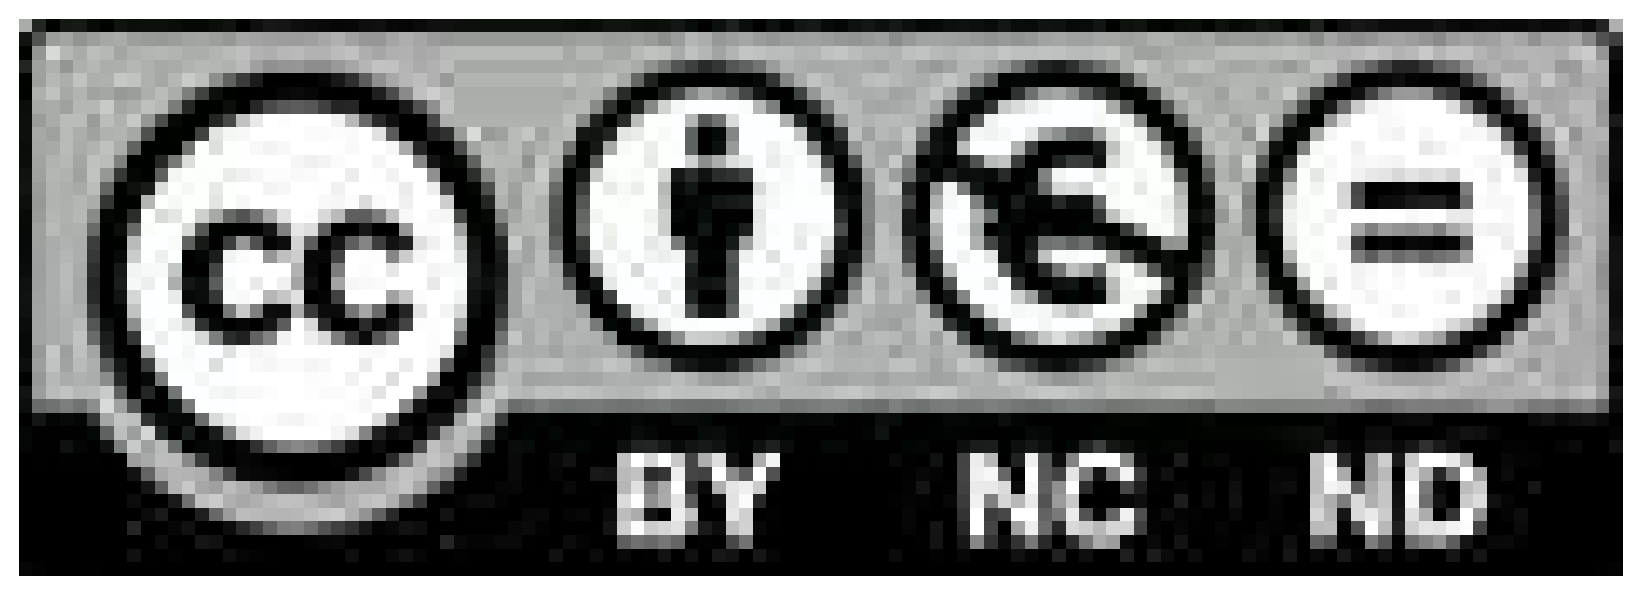
\includegraphics[width=0.2\textwidth]{Images/Cover/by-nc-nd}
\end{center}

This work is licensed under a Creative Commons Attribution-NonCommercial-NoDerivs License: 
\url{http://creativecommons.org/licenses/by-nc-nd/3.0/}
\\
\\
This work was partially funded by / Este trabajo fue parcialmente financiado por: \\
Consejer\'{i}a de Econom\'{i}a, Innovaci\'{o}n, Ciencia y Empresa. \\
Junta de Andaluc\'{i}a (Espa\~na)\\ 
Referencia: P07-TIC-03018}

\makeCover

%---------------------------------------------------------------------
%
%                          Certification
%
%---------------------------------------------------------------------
%
% certificacion.tex
% Copyright 2015 Dr. Francisco J. Pulido
%
% This file belongs to the PhD titled "New Techniques and Algorithms for Multiobjective and Lexicographic Goal-Based Shortest Path Problems", distributed under the Creative Commons Licence Attribution-NonCommercial-NoDerivs 3.0, available in http://creativecommons.org/licenses/by-nc-nd/3.0/. The complete PhD dissertation is freely accessible from http://www.lcc.uma.es/~francis/
%
% This thesis has been written adapting the TeXiS template, a LaTeX template for writting thesis and other documents. The complete TeXiS package can be obtained from http://gaia.fdi.ucm.es/projects/texis/. TeXis is distributed under the same conditions of the LaTeX Project Public License (http://www.latex-project.org/lppl.txt). The complete license is available in http://creativecommons.org/licenses/by-sa/3.0/legalcode
%
%---------------------------------------------------------------------

%---------------------------------------------------------------------
%
% Contiene el cap�tulo de la certificacion.
%
% Se crea como un cap�tulo sin numeraci�n.
%
%---------------------------------------------------------------------

%%%%%%%%%%%%%%%%%%%%%%%%%%%%%%%%%%%%%%%%%%%%%%%%%%%%%%%%%%%%%%%%%%%%%%
% Fecha de publicaci�n:
% \fechaPublicacion{Fecha}
% Puede ser vac�o. Aparece en la �ltima l�nea de la certificaci�n
%%%%%%%%%%%%%%%%%%%%%%%%%%%%%%%%%%%%%%%%%%%%%%%%%%%%%%%%%%%%%%%%%%%%%%
\lugarPublicacion{M\'alaga}

%%%%%%%%%%%%%%%%%%%%%%%%%%%%%%%%%%%%%%%%%%%%%%%%%%%%%%%%%%%%%%%%%%%%%%
% Fecha de publicaci�n:
% \fechaPublicacion{Fecha}
% Puede ser vac�o. Aparece en la certificaci�n
%%%%%%%%%%%%%%%%%%%%%%%%%%%%%%%%%%%%%%%%%%%%%%%%%%%%%%%%%%%%%%%%%%%%%%
\area{Ciencias de la Computaci�n e Inteligencia Artificial}


%%%%%%%%%%%%%%%%%%%%%%%%%%%%%%%%%%%%%%%%%%%%%%%%%%%%%%%%%%%%%%%%%%%%%%
% Titulaci�n:
% \titulacion{Fecha}
% Puede ser vac�o. Aparece en la certificaci�n
%%%%%%%%%%%%%%%%%%%%%%%%%%%%%%%%%%%%%%%%%%%%%%%%%%%%%%%%%%%%%%%%%%%%%%

\titulacion{Ingeniero en Inform�tica}

\makeCertif

%---------------------------------------------------------------------
%
%                          Dedication
%
%---------------------------------------------------------------------
%
% dedicatoria.tex
% Copyright 2015 Dr. Francisco J. Pulido
%
% This file belongs to the PhD titled "New Techniques and Algorithms for Multiobjective and Lexicographic Goal-Based Shortest Path Problems", distributed under the Creative Commons Licence Attribution-NonCommercial-NoDerivs 3.0, available in http://creativecommons.org/licenses/by-nc-nd/3.0/. The complete PhD dissertation is freely accessible from http://www.lcc.uma.es/~francis/
%
% This thesis has been written adapting the TeXiS template, a LaTeX template for writting thesis and other documents. The complete TeXiS package can be obtained from http://gaia.fdi.ucm.es/projects/texis/. TeXis is distributed under the same conditions of the LaTeX Project Public License (http://www.latex-project.org/lppl.txt). The complete license is available in http://creativecommons.org/licenses/by-sa/3.0/legalcode
%
%---------------------------------------------------------------------

%---------------------------------------------------------------------
%
% Contiene la p�gina de dedicatorias.
%
%---------------------------------------------------------------------

\dedicatoriaUno{%
\emph{
Para mis padres, \\
por su amor, dedicaci�n y sacrificios.
}%
}

%\dedicatoriaDos{%
%\emph{%
%I can't go to a restaurant and\\%
%order food because I keep looking\\%
%at the fonts on the menu.\\%
%Donald Knuth%
%}%
%}

\makeDedicatorias

%---------------------------------------------------------------------
%
%                          Acknowledgements
%
%---------------------------------------------------------------------
%
% agradecimientos.tex
% Copyright 2015 Dr. Francisco J. Pulido
%
% This file belongs to the PhD titled "New Techniques and Algorithms for Multiobjective and Lexicographic Goal-Based Shortest Path Problems", distributed under the Creative Commons Licence Attribution-NonCommercial-NoDerivs 3.0, available in http://creativecommons.org/licenses/by-nc-nd/3.0/. The complete PhD dissertation is freely accessible from http://www.lcc.uma.es/~francis/
%
% This thesis has been written adapting the TeXiS template, a LaTeX template for writting thesis and other documents. The complete TeXiS package can be obtained from http://gaia.fdi.ucm.es/projects/texis/. TeXis is distributed under the same conditions of the LaTeX Project Public License (http://www.latex-project.org/lppl.txt). The complete license is available in http://creativecommons.org/licenses/by-sa/3.0/legalcode
%
%---------------------------------------------------------------------

%---------------------------------------------------------------------
%
% Contiene la p�gina de agradecimientos.
%
% Se crea como un cap�tulo sin numeraci�n.
%
%---------------------------------------------------------------------

\chapter*{Agradecimientos}

\cabeceraEspecial{Agradecimientos}

Gracias, en primer lugar y de todo coraz�n, a mi tutor, el doctor Lawrence Mandow. Su paciencia, dedicaci�n y gu�a me han hecho llegar hasta donde estoy. �l, como ninguna otra persona, me ha ense�ado la pasi�n por la investigaci�n, el trabajo met�dico y la minuciosidad por los detalles. Ha sido un placer y un privilegio poder contar con su direcci�n y ayuda.

Gracias a Jos� Luis P�rez de la Cruz, catedr�tico de la Universidad de M�laga y una de las mentes m�s brillantes que conozco, por su inestimable ayuda y colaboraci�n. Su visi�n cr�tica y experiencia han contribuido a enriquecer los resultados de esta tesis.

Thanks to everyone in the University of Maths in Belgrade and the Computer Engineering and Informatics Department of the University of Patras. Dr. Du\v{s}an To\v{s}ic, Dr. Vladimir Filipovi\'{c}, Dr. Christos Zaroliagis, Nikos Rousias, Dimitris Gkortsilas and everyone else who made my PhD visits so enriching and enjoyable.

Gracias a mis compa�eros de laboratorio: Javi, Dani, Martyna, Rafa y todos aquellos con los que he compartido alegr�as y penas a lo largo de esta Tesis, y especialmente, a los doctores Enrique Machuca y Jaime G�lvez, por su desinteresada ayuda y su eterna disponibilidad. Esta Tesis Doctoral y mi tiempo en la Universidad no habr�an sido lo mismo sin ellos.

Gracias a la doctora Raquel Barco, por brindarme la oportunidad de dar un enfoque m�s comercial a los resultados de esta tesis. Gracias a Nacho, Juan, y el resto de mis compa�eros del proyecto de tr�fico inteligente por nuestras entretenidas reuniones diarias de sincronizaci�n. 

Y por encima de todo, y con todo mi amor, gracias a los m�os por estar incondicionalmente conmigo, por apoyarme siempre y sin restricciones. Gracias Mam�, Pap�, Mari, Lena y Runi. Os quiero mucho.


\begin{flushright}
\autor \\
\lugarPublicacionVal, \fechaPublicacionVal
\end{flushright}


\endinput

% Ponemos el marcador en el PDF al nivel adecuado, dependiendo
% de si hubo partes en el documento o no (si las hay, queremos
% que aparezca "al mismo nivel" que las partes.
\ifpdf
\ifx\tienePartesTeXiS\undefined
   \pdfbookmark[0]{Agradecimientos}{Agradecimientos}
\else
   \pdfbookmark[-1]{Agradecimientos}{Agradecimientos}
\fi
\fi


%---------------------------------------------------------------------
%
%                          Abstract
%
%---------------------------------------------------------------------
%
% abstract.tex
% Copyright 2015 Dr. Francisco J. Pulido
%
% This file belongs to the PhD titled "New Techniques and Algorithms for Multiobjective and Lexicographic Goal-Based Shortest Path Problems", distributed under the Creative Commons Licence Attribution-NonCommercial-NoDerivs 3.0, available in http://creativecommons.org/licenses/by-nc-nd/3.0/. The complete PhD dissertation is freely accessible from http://www.lcc.uma.es/~francis/
%
% This thesis has been written adapting the TeXiS template, a LaTeX template for writting thesis and other documents. The complete TeXiS package can be obtained from http://gaia.fdi.ucm.es/projects/texis/. TeXis is distributed under the same conditions of the LaTeX Project Public License (http://www.latex-project.org/lppl.txt). The complete license is available in http://creativecommons.org/licenses/by-sa/3.0/legalcode
%
%---------------------------------------------------------------------

\chapter*{Abstract}
\cabeceraEspecial{Abstract}

Shortest Path Problems (SPP) are one of the most extensively studied problems in the fields of Artificial Intelligence (AI) and Operations Research (OR). It consists in finding the shortest path between two given nodes in a graph such that the sum of the weights of its constituent arcs is minimized. However, real life problems frequently involve the consideration of multiple, and often conflicting, criteria. When multiple objectives must be simultaneously optimized, the concept of a single optimal solution is no longer valid. Instead, a set of efficient or Pareto-optimal solutions define the optimal trade-off between the objectives under consideration.  

The Multicriteria Search Problem (MSP), or Multiobjective Shortest Path Problem, is the natural extension to the SPP when more than one criterion are considered. The MSP is computationally harder than the single objective one. The number of label expansions can grow exponentially with solution depth, even for the two objective case \citep{hansen1979}. However, with the assumption of bounded integer costs and a fixed number of objectives the problem becomes tractable for polynomially sized graphs (e.g. see \citep{Mandow2009,Muller-Hannemann2006}).

A wide variety of practical application in different fields can be identified for the MSP, like robot path planning \citep{Wu2011}, hazardous material transportation \citep{caramiaetal2010}, route planning  \citep{Jozefowiez2008}, optimization of public transportation \citep{Raith2009}, QoS in networks \citep{craveirinha2009}, or routing in multimedia networks \citep{climacoetal2003}.

Goal programming is one of the most successful Multicriteria Decision Making (MCDM) techniques used in Multicriteria Optimization. In this thesis we explore one of its variants in the MSP. Thus, we aim to solve the Multicriteria Search Problem with lexicographic goal-based preferences. To do so, we build on previous work on algorithm \namoa, a successful extension of the \astar \ algorithm to the multiobjective case. More precisely, we provide a new algorithm called \lexgo, an exact label-setting algorithm that returns the subset of Pareto optimal paths that satisfy a set of lexicographic goals, or the subset that minimizes deviation from goals if these cannot be fully satisfied. Moreover, \lexgo \ is proved to be admissible and expands only a subset of the labels expanded by an optimal algorithm like \namoa, which performs a full Multiobjective Search.

Since time rather than memory is the limiting factor in the performance of  multicriteria search algorithms, we also propose a new technique called \emph{t-discarding} to speed up dominance checks in the process of discarding new alternatives during the search. The application of \emph{t-discarding} to the algorithms studied previously, \namoa \ and \lexgo, leads to the introduction of two new time-efficient algorithms named \namoate \ and \lexgote, respectively.

All the algorithmic alternatives are tested in two scenarios, random grids and realistic road maps problems. The experimental evaluation shows the effectiveness of \lexgo \ in both benchmarks, as well as the dramatic reductions of time requirements experienced by the t-discarding versions of the algorithms, with respect to the ones with traditional pruning.

\endinput



\ifx\generatoc\undefined
\else
%%---------------------------------------------------------------------
%
%                          TeXiS_toc.tex
%
%---------------------------------------------------------------------
%
% TeXiS_toc.tex
% Copyright 2009 Marco Antonio Gomez-Martin, Pedro Pablo Gomez-Martin
%
% This file belongs to TeXiS, a LaTeX template for writting
% Thesis and other documents. The complete last TeXiS package can
% be obtained from http://gaia.fdi.ucm.es/projects/texis/
%
% This work may be distributed and/or modified under the
% conditions of the LaTeX Project Public License, either version 1.3
% of this license or (at your option) any later version.
% The latest version of this license is in
%   http://www.latex-project.org/lppl.txt
% and version 1.3 or later is part of all distributions of LaTeX
% version 2005/12/01 or later.
%
% This work has the LPPL maintenance status `maintained'.
% 
% The Current Maintainers of this work are Marco Antonio Gomez-Martin
% and Pedro Pablo Gomez-Martin
%
%---------------------------------------------------------------------
%
% Contiene  los  comandos  para  generar los  �ndices  del  documento,
% entendiendo por �ndices las tablas de contenidos.
%
% Genera  el  �ndice normal  ("tabla  de  contenidos"),  el �ndice  de
% figuras y el de tablas. Tambi�n  crea "marcadores" en el caso de que
% se est� compilando con pdflatex para que aparezcan en el PDF.
%
%---------------------------------------------------------------------


% Primero un poquito de configuraci�n...

% Profundidad del indice de contenidos
\def\profTOCVal{3}
\newcommand{\profTOC}[1]{
\def\profTOCVal{#1}
}

% Profundidad de secciones que aparecen indice de contenidos
\def\profSecTOCVal{4}
\newcommand{\profSecTOC}[1]{
\def\profSecTOCVal{#1}
}

% Pedimos que inserte todos los ep�grafes hasta el nivel \subsection en
% la tabla de contenidos.
\setcounter{tocdepth}{\profTOCVal} 
%\setcounter{tocdepth}{2} 

% Le  pedimos  que nos  numere  todos  los  ep�grafes hasta  el  nivel
% \subsubsection en el cuerpo del documento.
\setcounter{secnumdepth}{\profSecTOCVal} 
%\setcounter{secnumdepth}{3} 



% Nombre de los indices de contenido
\def\indicesTOCVal{4}
\newcommand{\indicesTOC}[1]{
\def\indicesTOCVal{#1}
}

%  Nombre de la tabla de contenido
\def\tocNameVal{4}
\newcommand{\tocName}[1]{
\def\tocNameVal{#1}
}

%  Nombre de la lista de figuras
\def\lofNameVal{4}
\newcommand{\lofName}[1]{
\def\lofNameVal{#1}
}

%  Nombre de la lista de tablas
\def\lotNameVal{4}
\newcommand{\lotName}[1]{
\def\lotNameVal{#1}
}

%%%
%% COMANDO PARA CREAR LOS INDICES DE CONTENIDO
%% CONTIENE TODO EL C�DIGO LaTeX
%%%
\newcommand{\makeTOC}{

% Creamos los diferentes �ndices.

% Lo primero un  poco de trabajo en los marcadores  del PDF. No quiero
% que  salga una  entrada  por cada  �ndice  a nivel  0...  si no  que
% aparezca un marcador "�ndices", que  tenga dentro los otros tipos de
% �ndices.  Total, que creamos el marcador "�ndices".
% Antes de  la creaci�n  de los �ndices,  se a�aden los  marcadores de
% nivel 1.

\ifpdf
%   \pdfbookmark{�ndices}{indices}
   \pdfbookmark{\indicesTOCVal}{\indicesTOCVal}
\fi

% Tabla de contenidos.
%
% La  inclusi�n  de '\tableofcontents'  significa  que  en la  primera
% pasada  de  LaTeX  se  crea   un  fichero  con  extensi�n  .toc  con
% informaci�n sobre la tabla de contenidos (es conceptualmente similar
% al  .bbl de  BibTeX, creo).  En la  segunda ejecuci�n  de  LaTeX ese
% documento se utiliza para  generar la verdadera p�gina de contenidos
% usando la  informaci�n sobre los  cap�tulos y dem�s guardadas  en el
% .toc
\ifpdf
%   \pdfbookmark[1]{Tabla de contenidos}{tabla de contenidos}
   \pdfbookmark[1]{\tocNameVal}{\tocNameVal}
\fi

%\cabeceraEspecial{\'Indice}
\cabeceraEspecial{\tocNameVal}

\tableofcontents

\newpage 

% �ndice de figuras
%
% La idea es semejante que para  el .toc del �ndice, pero ahora se usa
% extensi�n .lof (List Of Figures) con la informaci�n de las figuras.

%\cabeceraEspecial{\'Indice de figuras}
\cabeceraEspecial{\lofNameVal}

\ifpdf
%   \pdfbookmark[1]{�ndice de figuras}{indice de figuras}
   \pdfbookmark[1]{\lofNameVal}{\lofNameVal}
\fi

\listoffigures

\newpage

% �ndice de tablas
% Como antes, pero ahora .lot (List Of Tables)

\ifpdf
%   \pdfbookmark[1]{�ndice de tablas}{indice de tablas}
   \pdfbookmark[1]{\lotNameVal}{\lotNameVal}
\fi

%\cabeceraEspecial{\'Indice de tablas}
\cabeceraEspecial{\lotNameVal}

\listoftables

\newpage

} %\newcommand{\makeTOC}

% Variable local para emacs, para  que encuentre el fichero maestro de
% compilaci�n y funcionen mejor algunas teclas r�pidas de AucTeX

%%%
%%% Local Variables:
%%% mode: latex
%%% TeX-master: "../Tesis.tex"
%%% End:

%---------------------------------------------------------------------
%
%                          Table of Contents
%
%---------------------------------------------------------------------
%
% toc.tex
% Copyright 2015 Dr. Francisco J. Pulido
%
% This file belongs to the PhD titled "New Techniques and Algorithms for Multiobjective and Lexicographic Goal-Based Shortest Path Problems", distributed under the Creative Commons Licence Attribution-NonCommercial-NoDerivs 3.0, available in http://creativecommons.org/licenses/by-nc-nd/3.0/. The complete PhD dissertation is freely accessible from http://www.lcc.uma.es/~francis/
%
% This thesis has been written adapting the TeXiS template, a LaTeX template for writting thesis and other documents. The complete TeXiS package can be obtained from http://gaia.fdi.ucm.es/projects/texis/. TeXis is distributed under the same conditions of the LaTeX Project Public License (http://www.latex-project.org/lppl.txt). The complete license is available in http://creativecommons.org/licenses/by-sa/3.0/legalcode
%
%---------------------------------------------------------------------

%---------------------------------------------------------------------
% Contiene  los  comandos  para  generar los  �ndices  del  documento,
% entendiendo por �ndices las tablas de contenidos.
%
% Genera  el  �ndice normal  ("tabla  de  contenidos"),  el �ndice  de
% figuras y el de tablas. Tambi�n  crea "marcadores" en el caso de que
% se est� compilando con pdflatex para que aparezcan en el PDF.
%
%---------------------------------------------------------------------

%%%%%%%%%%%%%%%%%%%%%%%%%%%%%%%%%%%%%%%%%%%%%%%%%%%%%%%%%%%%%%%%%%%%%%
% Profundidad del indice de contenidos:
% \profTOC{Valor}
% No Puede ser vac�o. 
%%%%%%%%%%%%%%%%%%%%%%%%%%%%%%%%%%%%%%%%%%%%%%%%%%%%%%%%%%%%%%%%%%%%%%
\profTOC{3}

%%%%%%%%%%%%%%%%%%%%%%%%%%%%%%%%%%%%%%%%%%%%%%%%%%%%%%%%%%%%%%%%%%%%%%
% Profundidad de secciones en indice de contenidos:
% \profSecTOC{Valor}
% No Puede ser vac�o. 
%%%%%%%%%%%%%%%%%%%%%%%%%%%%%%%%%%%%%%%%%%%%%%%%%%%%%%%%%%%%%%%%%%%%%%
\profSecTOC{4}

%%%%%%%%%%%%%%%%%%%%%%%%%%%%%%%%%%%%%%%%%%%%%%%%%%%%%%%%%%%%%%%%%%%%%%
% Nombre de los indices de contenido:
% \indicesTOC{Nombre}
% Puede ser vac�o. 
%%%%%%%%%%%%%%%%%%%%%%%%%%%%%%%%%%%%%%%%%%%%%%%%%%%%%%%%%%%%%%%%%%%%%%
\indicesTOC{Indexes}

%%%%%%%%%%%%%%%%%%%%%%%%%%%%%%%%%%%%%%%%%%%%%%%%%%%%%%%%%%%%%%%%%%%%%%
% Nombre de la tabla de contenido:
% \tocName{Nombre}
% Puede ser vac�o. 
%%%%%%%%%%%%%%%%%%%%%%%%%%%%%%%%%%%%%%%%%%%%%%%%%%%%%%%%%%%%%%%%%%%%%%
\tocName{Table of Contents}

%%%%%%%%%%%%%%%%%%%%%%%%%%%%%%%%%%%%%%%%%%%%%%%%%%%%%%%%%%%%%%%%%%%%%%
% Nombre de la lista de figuras:
% \lofName{Nombre}
% Puede ser vac�o. 
%%%%%%%%%%%%%%%%%%%%%%%%%%%%%%%%%%%%%%%%%%%%%%%%%%%%%%%%%%%%%%%%%%%%%%
\lofName{List of Figures}

%%%%%%%%%%%%%%%%%%%%%%%%%%%%%%%%%%%%%%%%%%%%%%%%%%%%%%%%%%%%%%%%%%%%%%
% Nombre de la lista de tablas:
% \lotName{Nombre}
% Puede ser vac�o. 
%%%%%%%%%%%%%%%%%%%%%%%%%%%%%%%%%%%%%%%%%%%%%%%%%%%%%%%%%%%%%%%%%%%%%%
\lotName{List of Tables}

\makeTOC


\fi

% Marcamos el  comienzo de  los cap�tulos (para  la numeraci�n  de las
% p�ginas) y ponemos la cabecera normal
\mainmatter
\restauraCabecera

\bibliographystyle{TeXiS/TeXiS}

%---------------------------------------------------------------------
%
%                          Part Intro
%
%---------------------------------------------------------------------
%
% PartIntro.tex
% Copyright 2015 Dr. Francisco J. Pulido
%
% This file belongs to the PhD titled "New Techniques and Algorithms for Multiobjective and Lexicographic Goal-Based Shortest Path Problems", distributed under the Creative Commons Licence Attribution-NonCommercial-NoDerivs 3.0, available in http://creativecommons.org/licenses/by-nc-nd/3.0/. The complete PhD dissertation is freely accessible from http://www.lcc.uma.es/~francis/
%
% This thesis has been written adapting the TeXiS template, a LaTeX template for writting thesis and other documents. The complete TeXiS package can be obtained from http://gaia.fdi.ucm.es/projects/texis/. TeXis is distributed under the same conditions of the LaTeX Project Public License (http://www.latex-project.org/lppl.txt). The complete license is available in http://creativecommons.org/licenses/by-sa/3.0/legalcode
%
%---------------------------------------------------------------------

\partTitle{Motivation and Fundamentals}

\partDesc{This first part of this thesis is divided into three chapters. The first one is devoted to introduce its field of study. We enumerate the goals of this dissertation and introduce the contributions that we will develop further in the second part. The second chapter describes our main subject of study and research, Multicriteria Search problems and algorithms. The third chapter is dedicated to the benchmarks used to conduct the experimental evaluation. Thus, in particular: 

\begin{itemize}
    \item Chapter \ref{chapIntroduction} gives an overview of the motivation, scope and goals of this thesis, and enumerates its contributions.  
    \item Chapter \ref{chapMultiObjAlg} defines the Multicriteria Search Problem, gives some examples of application and classifies the approaches to deal with the problem. Formal properties of the lower bounds to apply to the multicriteria search algorithms are also described. Finally, \namoa \ is introduced emphasizing its relevant features and properties to our own work.
    \item Chapter \ref{chapMultiObjTestBeds} enumerates relevant benchmarks employed in the literature and describes the test beds used in this thesis, as well as the main parameters followed in the experimental evaluation.
\end{itemize}
}

\makepart

%---------------------------------------------------------------------
%
% Chapter 1: Introduction
%
%---------------------------------------------------------------------
%
% ChapIntroduction.tex
% Copyright 2015 Dr. Francisco J. Pulido
%
% This file belongs to the PhD titled "New Techniques and Algorithms for Multiobjective and Lexicographic Goal-Based Shortest Path Problems", distributed under the Creative Commons Licence Attribution-NonCommercial-NoDerivs 3.0, available in http://creativecommons.org/licenses/by-nc-nd/3.0/. The complete PhD dissertation is freely accessible from http://www.lcc.uma.es/~francis/
%
% This thesis has been written adapting the TeXiS template, a LaTeX template for writting thesis and other documents. The complete TeXiS package can be obtained from http://gaia.fdi.ucm.es/projects/texis/. TeXis is distributed under the same conditions of the LaTeX Project Public License (http://www.latex-project.org/lppl.txt). The complete license is available in http://creativecommons.org/licenses/by-sa/3.0/legalcode
%
%---------------------------------------------------------------------

\chapter{Introduction}
\label{chapIntroduction}


\begin{FraseCelebre}
\begin{Frase}
Research is what I'm doing when I don't know what I'm doing
\end{Frase}
\begin{Fuente}
Wernher von Braun (1912-1977)
\end{Fuente}
\end{FraseCelebre}
%
%\begin{resumen}
%...
%\end{resumen}

This doctoral dissertation falls within the scope of the Artificial Intelligence (AI) and Operations Research (OR) fields. Shortest Path Problems (SPP) are one of the oldest and most extensively studied problems in both fields, which consists in finding the shortest path between two given nodes in a graph such that the sum of the weights of its constituent arcs is minimized. The SPP arises naturally in real life, e.g. planning the route path in a road trip, or navigating a mobile robot to avoid obstacles, and can be also used to solve optimally puzzle games like Rubik's cube \citep{Korf1997} or the twenty-four puzzle \citep{Korf1996}.

The Multicriteria Search Problem (MSP), or Multiobjective Shortest Path Problem, is the natural extension to the SPP whenever more than one criterion is considered. The MSP is computationally harder than the single objective one. The number of label expansions can grow exponentially with solution depth, even for the two objective case \citep{hansen1979}. With the assumption of bounded integer costs and a fixed number of objectives the problem becomes tractable for polynomially sized graphs, but still harder than single objective search (e.g. see \citep{Mandow2009,Muller-Hannemann2006}).

Recent experiments on problems like bicriteria route planning have revealed that time, rather than space, is the practical limiting factor in the calculation of the full set of efficient solutions in exact algorithms in Multicriteria Search \citep{Machuca2011b, Machuca2009}. In this thesis we address this problem from the point of view of Goal Programming (GP), which has proven to be a very effective model of decision maker's preferences over multicriteria decision making (MCDM) problems. Goal Programming is a general paradigm which claims that a decision problem can be expressed through a set of goals defined by the decision maker, rather than through the optimization of a set of objectives. Roughly speaking, a goal defines a degree of satisfaction of a given criteria that is deemed satisfactory or acceptable by the decision maker. One of the most commonly used schemes to express goal-based preferences is the lexicographic method of grouping criteria by pre-emptive importance \citep{Charnes1977,Romero1991}.

Our starting hypothesis is that in those cases where user preferences can be initially bounded by a set of goals, specially designed search algorithms could perform more efficiently than searching for the full Pareto frontier. The main goals of this thesis are to explore this hypothesis, and to improve the performance of current multiobjective search algorithms. More precisely, we explore new algorithmic contributions to the MSP with lexicographic goal-based preferences, and also a new technique to speed up multicriteria search algorithms based on labeling techniques.    

Section \ref{ChapIntroduction:sec:motivation} introduces the motivation and significance of this work for the AI and OR fields. Section \ref{ChapIntroduction:sec:orientation} presents our scope and orientation. The goals and contributions of this thesis are enumerated in Sections \ref{ChapIntroduction:sec:objectives} and \ref{ChapIntroduction:sec:contributions}, respectively. Related publications of this research work are shown in Section \ref{ChapIntroduction:sec:publications}. Finally, Section \ref{ChapIntroduction:sec:outline} outlines the structure of this thesis.

%-------------------------------------------------------------------
\section{Motivation}
\label{ChapIntroduction:sec:motivation}
%-------------------------------------------------------------------

The Shortest Path Problem is a recurrent problem in the AI and OR literature. \citet{dijkstra1959} proposed the first algorithm to find the minimal cost route between two nodes in a graph. The A$^*$ algorithm \citep{Hart1968} is an important algorithmic reference that exploits specific problem knowledge (the so-called heuristic function in the AI community) to guide the search and improve its efficiency. This problem knowledge is in the form of a distance or cost estimate.

Real life decision problems frequently involve the consideration of multiple criteria simultaneously. For example, Figure \ref{ChapIntroduction:fig:sample-app} shows three car routes from M\'{a}laga to Valencia (both in Spain) suggested by a sample web application devoted to road route planning. Assume we are concerned with the minimization of three different criteria in this problem: travel cost, time and distance. Route \ref{ChapIntroduction:fig:sample-app-1} is the fastest and shortest route and Route \ref{ChapIntroduction:fig:sample-app-3} is the cheapest. Whenever there are no other preferences defined, we say that both routes are \emph{efficient solutions} to this problem, i.e. these solutions represent an optimal trade-off between the criteria. These are extreme efficient solutions, but there might well be other interesting trade-offs. The set of all solutions such that none of the objectives can be improved without worsening at least one of the others, is called the Pareto set or Pareto frontier, and they are call efficient or non-dominated solutions.

\begin{figure}
    \begin{center}
      \subfigure[Route 1]{\label{ChapIntroduction:fig:sample-app-1}
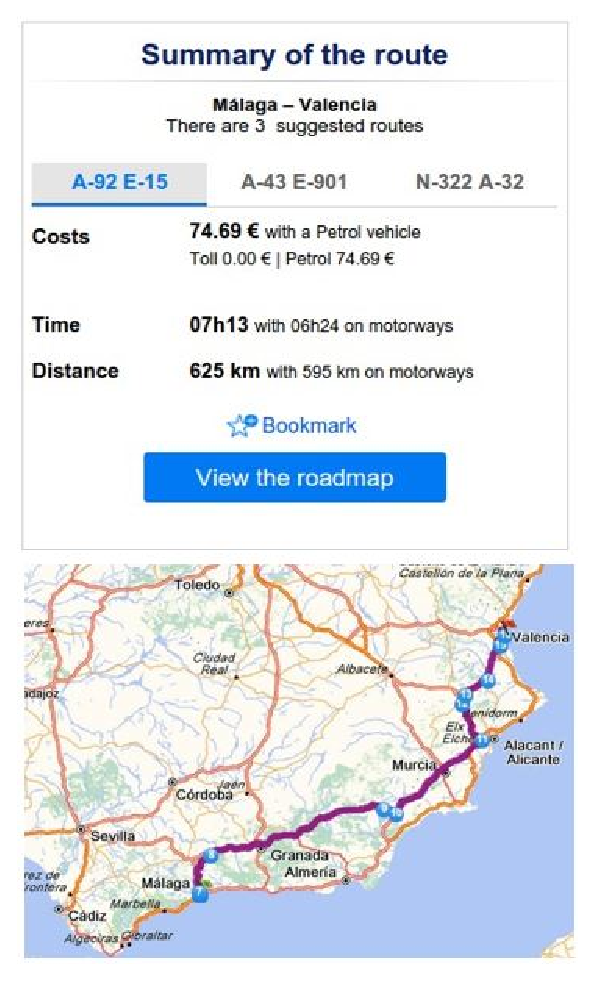
\includegraphics[width=0.3\textwidth]{Images/Chapter1/sample-app-1}
        }
        \subfigure[Route 2]{ \label{ChapIntroduction:fig:sample-app-2}
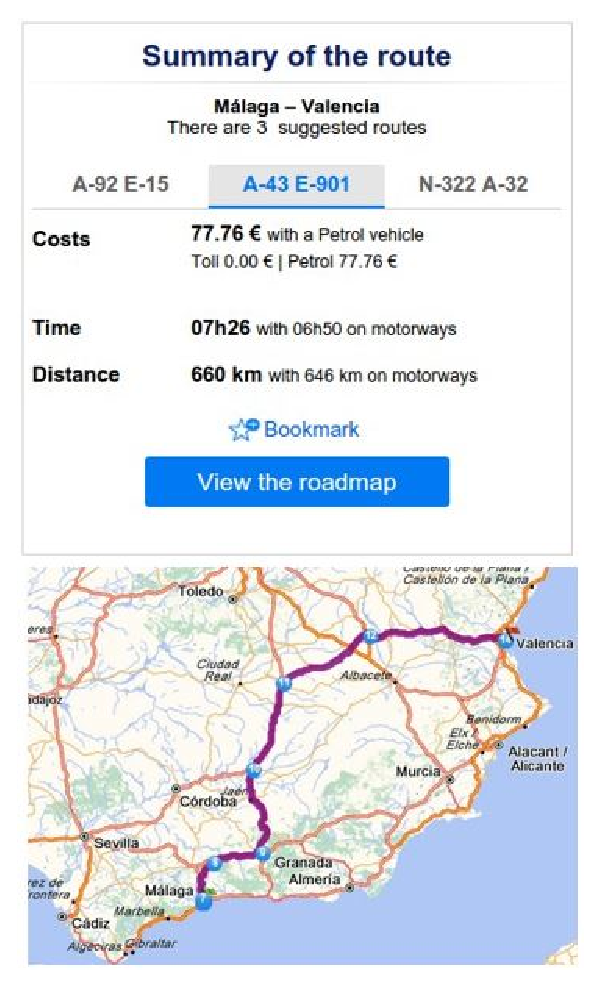
\includegraphics[width=0.3\textwidth]{Images/Chapter1/sample-app-2}
        }
       \subfigure[Route 3]{\label{ChapIntroduction:fig:sample-app-3}
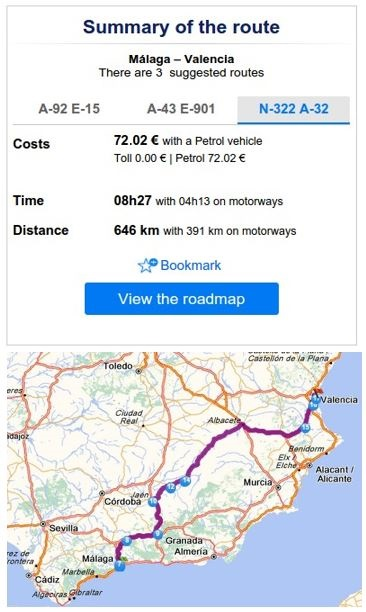
\includegraphics[width=0.3\textwidth]{Images/Chapter1/sample-app-3}
        }
    \end{center}
    \vspace{-0.25in} 
    \caption{
      Screenshots from a sample route planning web application, showing alternative routes from M\'{a}laga (Spain) to Valencia (Spain). \copyright \ \url{www.viamichelin.com}
    }
    \label{ChapIntroduction:fig:sample-app}
\end{figure}

Among all feasible routes in our example only a subset can be considered non-dominated in terms of all objectives. Thus, route \ref{ChapIntroduction:fig:sample-app-2} is called a dominated solution, since there is another route, route \ref{ChapIntroduction:fig:sample-app-1}, that is lower in all objectives. However, the calculation of the Pareto set is typically a hard problem, hence, we consider the application of Goal Programming (GP) to model the decision maker's preferences and establish a set of goals that  restrict the set of solutions to those ones which satisfy those goals, or which minimize the deviation from the goals if they can not be satisfied. Thus, in our example, a user of the road route planner can define their expectations of the maximum economic cost, time and distance for the trip.

In order to deal with the problem described above, two different alternatives can be followed. In the first one, a full Multicriteria Search algorithm can return the full Pareto set of solutions to the problem. This set can then be used to determine the subset of solutions that satisfy the goals, or in case the goals can not be fully satisfied, the subset which minimizes the deviation from those goals according to a given definition of distance. For this alternative, we consider \namoa, which is currently the most efficient exact algorithm to calculate the Pareto frontier.

The second alternative to deal with the MSP with goal-based preferences concentrates the search effort on the subset of Pareto optimal solutions that satisfy the goals, discarding those paths that will not lead to efficient solutions according to the goals. Notice that we shall always seek for efficient or non-dominated solutions for the problem, regardless whether the goals can be satisfied or not. This is not the case of Goal Programming in general, that allows non-dominated solutions to the problem. 

For the second alternative, we introduce \lexgo, a best-first Multicriteria Search algorithm that is also exact and efficient when provided with consistent lower bounds. 

Finally, this thesis is also devoted to improve the time performance of exact multicriteria search algorithms with consistent lower bounds and to do so, a new dimensionality reduction technique is introduced. This technique allows discarding non-dominated paths with a dramatic decreased number of dominance checks against permanent labels. Its application to \namoa \ and \lexgo \ leads to the introduction of two new algorithms, \namoate \ and \lexgote. Their effectiveness is also studied from formal and empirical points of view against traditional pruning or discarding.  

%-------------------------------------------------------------------
\section{Scope and Orientation}
\label{ChapIntroduction:sec:orientation}
%-------------------------------------------------------------------

We summarize the boundaries of this doctoral dissertation with the following terms:

\begin{description}
	
	\item[Multicriteria Search with lower bounds.] The Shortest Path Problem consists in finding the shortest path between two nodes in a graph. The natural extension when considering multiple conflicting criteria is the Multicriteria Search Problem. We consider the $A^*$ algorithm as a reference in the solution of this problem and, therefore, analyze multicriteria search algorithms whose
performance can improve with the use of lower bounds or distance estimates to restrict the number of label expansions.
	
	\item[Additive costs.] Arcs in the graph are labeled with a magnitude for each criterion, or cost, under consideration. In the MSP, the arcs in the graph represent the costs of navigating from the source to the destination node. The cost of the route in the graph to be minimized corresponds to the sum of the costs vectors of its component arcs. 
	
	\item[Pareto optimality.] When multiple criteria are considered, the concept of minimum no longer applies, and is usually replaced by that of Pareto optimality. Pareto optimal solutions are defined as those that cannot be improved according to one objective without worsening at least one of the others.
	
	\item[Label-setting multicriteria search algorithms.] 
Best-first algorithms are classified in the OR literature as label-setting or label-correcting. The former explores only optimal paths in the graph, and therefore set permanent labels for each scanned node. The latter may also explore suboptimal paths and therefore may establish temporary labels for scanned nodes. When algorithms A$^*$ or \namoa \ use consistent lower bounds as cost estimates, they behave as label-setting algorithms. That will also be the case for the algorithms analyzed in this thesis.
	
	\item[Pre-emptive and weighted preferences.] 
Goal Programming models preferences given by a decision maker for a multicriteria problem. We focus on the technique where the criteria are grouped in priority levels sorted in order of decreasing pre-emptive importance. Furthermore, a level comprises a set of one or more attributes. We define targets for each attribute and weights to establish the importance of the criteria within the level. 

	\item[Theoretical proofs of correctness.] We contribute in this thesis several new algorithms. Formal proofs of their admissibility and efficiency are provided. These are complemented with empirical analyses of the algorithms.

\end{description}

%-------------------------------------------------------------------
\section{Research Goals}
\label{ChapIntroduction:sec:objectives}
%-------------------------------------------------------------------

The main goals of this doctoral dissertation can be outlined as follows:

\begin{enumerate}
	\item \textbf{Address the Multicriteria Search Problem with goal-based preferences.} The first goal of this thesis is the description of the Multicriteria Search Problem and specifically, the Multicriteria Search Problem with Preferences Based on Goals. We will describe the two considered approaches to deal with such a problem in detail. 

	\item \textbf{Devise a new algorithm to cope with lexicographic goal-based preferences.} The principle of optimality holds for Multiobjective Shortest Path Problems, but regrettably does not hold for lexicographic goal-based preferences. In order to approach the MSP with a specifically designed goal-based algorithm, we concentrate our efforts to devise a new algorithm  based on a label selection policy.  

	\item \textbf{Prove formally the correctness and efficiency of this new algorithm.} Another goal of this thesis is to complement the defined algorithm with formal analyses of its correctness as well as its efficiency over an optimal algorithm that performs a full Multiobjective Search (\namoa).	

	\item \textbf{Study possible improvements to multiobjective shortest path algorithms.} Our efforts will also be focused on the improvement of multiobjective shortest path algorithms in general. More specifically, we aim to introduce a new dimensionality reduction technique to improve the runtime performance of label-setting multiobjective shortest path algorithms with consistent lower bounds.

	\item \textbf{Prove formally the correctness of the dimensionality reduction technique.} We will formally develop the application of the dimensionality reduction technique to the new defined algorithm based on goal preferences, as well as the application to \namoa. In particular, we will prove theoretically the correctness of both algorithms when employing the dimensionality reduction technique.

	\item \textbf{Perform an empirical evaluation of all the algorithmic alternatives.} Finally, the last goal of this dissertation is to provide an extensive evaluation of all the proposed algorithms. We will employ test beds over randomly generated and realistic scenarios.
\end{enumerate}

%-------------------------------------------------------------------
\section{Contributions}
\label{ChapIntroduction:sec:contributions}
%-------------------------------------------------------------------
 
The contributions of this thesis are enumerated as follows: 

\begin{enumerate}
	\item \textbf{Description of the Goal-Based Multicriteria Graph Search Problem.} In the first place, we outline the Goal Programming technique within the Multicriteria Decision Making discipline. We also outline the Multicriteria Graph Search within the Multiobjective Optimization Problem, and given that framework, we will describe and define formally the Goal-Based Multicriteria Graph Search problem and the different algorithmic approaches to deal with it.  

	\item \textbf{A new Multicriteria Search algorithm for the MSP.} We introduce \lexgo \ (Lexicographic Goals A$^*$), a new exact label-setting algorithm for Multicriteria Search problems with goal-based preferences. \lexgo \ returns the subset of non-dominated optimal paths that satisfy a set of lexicographic goals, or the subset that minimizes deviation from goals if these cannot be fully satisfied.

	\item \textbf{Formal characterization of the admissibility and efficiency of \lexgo.} We prove theoretically the admissibility of \lexgo, i.e. the algorithm is exact and returns the whole set of solutions to the problem, as well as its efficiency, i.e. the number of labels scanned by the algorithm decreases with better (more informed) lower bounds, over the full Multicriteria Search.

	\item \textbf{Introduction of \emph{t-discarding}.} We introduce a new dimensionality reduction technique called \emph{t-discarding}. This technique can be applied to the processes of pruning and filtering in order to reduce in one dimension the size of the vectors considered to discard new alternatives. Thus, we will reduce the amount of time needed to check dominance against closed vectors and therefore, the time requirements of the algorithms.

	\item \textbf{Formal characterization of the t-discarding technique.} We apply t-discarding to \namoa \ and \lexgo, introduce new algorithms \namoate \ and \lexgote, show their correctness, evaluate their effectiveness, and analyze their performance.  

	\item \textbf{Empirical evaluation of the new algorithmic contributions.} Two main scenarios are used to test the effectiveness of our devised algorithms, random grids and realistic road maps problems. We present dramatic reduction in time requirements for three-objective, four-objective and five-objective search problems over random grids. To the best of our knowledge, the results reported over road maps problems represent the largest three-objective search problems solved to date. 		
\end{enumerate}

%-------------------------------------------------------------------
\section{Related Publications}
\label{ChapIntroduction:sec:publications}
%-------------------------------------------------------------------

Contributions of this thesis has been presented in international peer-reviewed journals and conferences.

\begin{itemize}

    \item \textbf{\large Journals:}
\par
Pulido, F. J., Mandow, L., \& P\'{e}rez de la Cruz, J. (2014). Multiobjective shortest path problems with lexicographic goal-based preferences. European Journal of Operational Research, 239(1), 89-101. doi:10.1016/j.ejor.2014.05.008
\par 
Pulido, F. J., Mandow, L., \& P\'{e}rez de la Cruz, J. (2015). Dimensionality reduction in multiobjective shortest path search. Computers \& Operations Research. Volume 64, 60-70. doi:10.1016/j.cor.2015.05.007
%
    \item \textbf{\large Conferences:}
\par
Mandow, L., Pulido, F. J., \& P\'{e}rez de la Cruz, J. L. (2013). Searching Graphs with Lexicographic Goal Preferences. In 22nd International Conference on Multiple Criteria Decision Making - MCDM 2013.

\end{itemize}

%-------------------------------------------------------------------
\section{Outline}
\label{ChapIntroduction:sec:outline}
%-------------------------------------------------------------------

This doctoral dissertation is structured in eight chapters grouped in three parts. The first part is devoted to present the motivation of this thesis, its foundations and previous work, and comprises this introductory chapter, and Chapters \ref{chapMultiObjAlg} and \ref{chapMultiObjTestBeds}. Chapter \ref{chapMultiObjAlg} introduces the reader to the Multicriteria Search Problem with lexicographic goal-based preferences. Relevant models of decision maker's preferences are enumerated and several practical applications are described. This chapter also introduces the fundamentals of Multicriteria Search Problems, reviews different kinds of multiobjective search methods, and presents \namoa, the reference algorithm we use to evaluate our contributions under a common framework. Chapter \ref{chapMultiObjTestBeds} briefly reviews previous relevant multiobjective benchmarks. A set of good practices in the experimental evaluation of algorithms as well as the key concepts to measure the performance of Multicriteria Search are also presented. Finally, benchmarks employed in this thesis are described in detail. 

The second part of this dissertation groups the main contributions of this thesis. Chapter \ref{chapContributions} presents 
%relevant new definitions of lexicographic preferences and dominance checks, as well as 
the new algorithms \lexgo, \namoate \ and \lexgote. Chapter \ref{chapFormalAnalysis} gives a formal analysis of the algorithms devised as a result of this thesis, and presents the proofs for their properties of exactness and efficiency, i.e. it is formally proved for each algorithm in this thesis that the full set of efficient solutions is returned and the number of explored labels decreases with more informed lower bounds. Chapters \ref{chapEmpiricalAnalysisGrids} and \ref{chapEmpiricalAnalysisRoadMaps} analyze the performance of all the algorithmic alternatives over random grids and realistic road maps problems, respectively. These reveal the effectiveness of the proposed techniques.

Finally, part three summarizes the conclusions of this thesis and introduces future lines of work in Chapter \ref{ChapConclusions}.

%---------------------------------------------------------------------
%
% Chapter 2: Multicriteria Graph Search
%
%---------------------------------------------------------------------
%
% ChapMultiObjAlg.tex
% Copyright 2015 Dr. Francisco J. Pulido
%
% This file belongs to the PhD titled "New Techniques and Algorithms for Multiobjective and Lexicographic Goal-Based Shortest Path Problems", distributed under the Creative Commons Licence Attribution-NonCommercial-NoDerivs 3.0, available in http://creativecommons.org/licenses/by-nc-nd/3.0/. The complete PhD dissertation is freely accessible from http://www.lcc.uma.es/~francis/
%
% This thesis has been written adapting the TeXiS template, a LaTeX template for writting thesis and other documents. The complete TeXiS package can be obtained from http://gaia.fdi.ucm.es/projects/texis/. TeXis is distributed under the same conditions of the LaTeX Project Public License (http://www.latex-project.org/lppl.txt). The complete license is available in http://creativecommons.org/licenses/by-sa/3.0/legalcode
%
%---------------------------------------------------------------------

\chapter{MultiCriteria Graph Search}
\label{chapMultiObjAlg}

%
\begin{FraseCelebre}
\begin{Frase}
It is not the task of the University to offer what society asks for, but to give what society needs.	
\end{Frase}
\begin{Fuente}
Edsger Dijkstra (1930-2002)
\end{Fuente}
\end{FraseCelebre}

This chapter has a twofold purpose, on one hand, provide an overview of two opposite decision paradigms: optimization and satisfaction. On the other hand, deepen insight into the Multicriteria Search Problem (MSP), present the state of the art in algorithms to deal with such problems, and delimit the frame of the algorithms studied in this thesis.

An optimization problem is the problem of finding the best solution from all feasible solutions. This process is suitable for developing computational algorithms that optimize the decision according to given criteria, although in certain cases cannot be appropriate due to its greater computational requirements to solve problems. Humans, however, do not pursue the optimization of their decisions in general. This is where the concept of satisfaction emerges. A satisfactory solution from this perspective is any feasible solution that fulfills the standards or goals of the decision maker. We will further elaborate on both decision paradigms in this Chapter. 

The Multicriteria Decision Making (MCDM) discipline is introduced in the first place in Section \ref{chapMultiObjAlg:sec:MCDM}. Both decision paradigms explained above are part of this discipline. Then, the Multiobjective Optimization Problem (MOP) is presented in Section \ref{chapMultiObjAlg:sec:MOP} along with a classification of the main methods to deal with it. 

Goal Programming (GP), see Section \ref{chapMultiObjAlg:sec:GP}, is a popular method for dealing with multiple objective decision-making problems based on satisfying the goals of a decision maker. GP is a branch of Multicriteria Decision Making that aims to ``satisfice'' instead of optimize. The most popular variants of GP preference modeling are described in Section \ref{chapMultiObjAlg:subsec:GP-variants}. Among them, we focus on Lexicographic GP and introduce relevant definitions concerning this modeling tool in Section \ref{chapMultiObjAlg:subsec:lex-MOP}.

This thesis tackles the Shortest Path Problem with multiple criteria. Prior to defining the MSP, the Shortest Path Problem is defined in Section \ref{chapMultiObjAlg:sec:SPP} along with the most well known approaches to solve it. Right after, the MSP is presented in Section \ref{chapMultiObjAlg:sec:MSP}, as well as a wide range of fields where the MSP has been applied successfully. Sections \ref{chapMultiObjAlg:sec:a-posteriori} and \ref{chapMultiObjAlg:sec:a-priori} analyze the two main algorithmic approaches to solve a MSP, classified depending on the a priori or a posteriori character of the decision maker's preferences. In the first case, we will further study the class of best-first algorithms, and in particular, the state-of-the-art algorithm \namoa. In the second case, we review research on multicriteria search algorithms that can provide compromise solutions or solutions according to some targets.

Finally, Section \ref{chapMultiObjAlg:sec:summary}, summarizes the key concepts of this given chapter, and introduces the motivation and contributions of this research work.

%-------------------------------------------------------------------
\section{Multicriteria Decision Making}
\label{chapMultiObjAlg:sec:MCDM}
%-------------------------------------------------------------------

Multicriteria Decision Making (MCDM), also called Multicriteria Decision Analysis (MCDA), is a sub-discipline of the field of Operations Research. MCDM is a paradigm that involves the consideration of multiple, and in general conflicting, criteria in decision-making environments. In real life problems, there are typically multiple conflicting criteria that need to be evaluated in making decisions. The purpose of MCDM is to support decision makers (an individual or a group of individuals) to make those decisions. Typically, there does not exist a unique optimal solution for such problems and it is necessary to use the decision maker's (DM) preferences to select between solutions. For instance, when buying a new computer, cost, performance and design may be some of the main criteria a buyer considers. It is unusual to have the cheapest computer to be the best designed and the most powerful. 

%According to Dr. Carlos Romero, a formal definition of MCDM is: "Set of mathematical methods and computational techniques that with an explicative, normative or prescriptive purpose, aim to assess a finite and explicite (discrete case) or an infinite number of alternatives based upon a finite number of criteria"

Solving a MCDM problem can be interpreted in different ways. A decision maker can seek the "most preferred" alternative, i.e. the best alternative from a set of available alternatives. Another interpretation could be choosing a small set of good alternatives, or grouping alternatives into different preference sets. Finally, the last interpretation could be to find all \textit{efficient} or \textit{non-dominated} alternatives. 

Let us first introduce some relevant concepts taken from \citep{Romero1991,Romero1993}: 

\begin{defi}\label{defi:attribute}
Zeleny \citep{Zeleny1982} and Romero define \textbf{attributes} as descriptors of an objective reality to represent values of the DMs. These values are measurable properties that can be expressed as a mathematical function $g(\vec x): X \rightarrow \mathbb{R}$, where $\vec x$ is the vector of the decision variables and $X$ is the set of solutions to the decision problem. 
\end{defi}

\begin{defi}\label{defi:objective}
\textbf{Objectives} represent the desired improvement of an attribute, i.e. the maximization or the minimization of the mathematical functions corresponding to the attributes under consideration. In short, objectives take the form: $\max g(\vec x)$ or $\min g(\vec x)$.
\end{defi} 

\begin{defi}\label{defi:targetgoal}
A \textbf{target} or aspiration level, $t \in \mathbb{R}$, is an acceptable level of achievement for any of the attributes considered by the DM. A \textbf{goal} is a combination of an attribute with a target, stated by the decision maker to define their preference. 
\end{defi}

\begin{defi}\label{defi:deviation}
A \textbf{deviation variable} represents the distance between the \textit{i-th} goal and its associated aspiration level. A formulation model is defined as the minimization of the deviation variables to achieve the goals. Three different kinds of goals are defined in this context. In each of them we select different deviation variables to minimize. Table \ref{tab:deviation-variables} shows the concept of unwanted deviation variable, or variable to minimize, depending on the kind of goal.

\begin{table}
\caption{Goals and deviation variables (taken from \citep{Romero1993}.}
\centering
\begin{tabular}{ccc}
\hline \noalign{\smallskip}
Type of objective function & Goal type & Deviation to minimize\\
\noalign{\smallskip} \hline
Minimization & $g_i(\vec x) \leq t_i$ & $d_i$ \\
Maximization & $g_i(\vec x) \geq t_i$ & $p_i$ \\
Exact achievement & $g_i(\vec x) = t_i$ & $d_i + p_i$ \\
\hline
\end{tabular}
\label{tab:deviation-variables}
\end{table}  

The distance between the \emph{i-th} goal and its associated aspiration level may be negative (represented by $d_i$) or positive (represented by $p_i$). A negative value represents the number of units in which the \textit{i-th} goal falls below with respect to the target defined. The positive value represents just the opposite, i.e. the number of units in which the achievement of the \textit{i-th} goal has been surpassed regarding the aspiration level proposed. In general, the \textit{i-th} goal expressed algebraically is, 
\begin{equation}\label{eq:goal-mat}
g_i(x) + d_i - p_i = t_i \qquad d_i, p_i \geq 0
\end{equation}
\end{defi}

\begin{defi}\label{defi:criterion}
The term \textbf{criterion} comprises attributes, objectives and goals of a DM relevant to a particular decision-making problem.
\end{defi}

\citet{Romero1993} splits the MCDM framework into two scenarios. The first one corresponds to a decision making situation with a discrete number of feasible solutions to be ranked according to different attributes. In this case a multiattribute utility function represents the preferences of the DM and is used to order the set of finite feasible alternatives. This approach is called Multiattribute Decision Making (MADM) (see for example \citep{tzeng2011}).

The second scenario corresponds to a decision making situation with an infinite number of decision alternatives where the practical possibility of obtaining a reliable representation of the DM's utility function is very limited. In this case with multiple objectives the Multiobjective Optimization, also known as  Multiobjective Programming (MOP), is the approach to consider. In general, a Multiobjective Optimization problem assumes a simple preference structure, the so-called Pareto ordering \citep{Pareto1897}, to find the set of trade-offs between all objectives considered \citep{ChankongHaimes1983}.

Let us now revise a formal definition of the Multiobjective Optimization Problem, introduce definitions relevant to this research work, and classify the most popular techniques to deal with it.

%-------------------------------------------------------------------
\section{Multiobjective optimization}
\label{chapMultiObjAlg:sec:MOP}
%-------------------------------------------------------------------

Let us first introduce a mathematical formulation of the Multiobjective Optimization Problem, 

\begin{defi}\label{chapMultiObjAlg:def:multiObjProb}
Let $X$ be the set of feasible solutions to a problem and let $f^k:X \rightarrow \mathbb{R}$ be $k$ functions assigning a real value as image to a solution in $X$, being $k \in \{1,2,\ldots ,q \}$ objectives. A multiobjective problem in $X$ can be formulated as a minimization problem,
\begin{eqnarray}\label{chapMultiObjAlg:eq:probMultiObj}
     \min \vec f(\vec x)=(f^1(\vec x),f^2(\vec x),\ldots ,f^q(\vec x)) \\
\nonumber \raggedleft	  s.t. \ \vec x \in X
\label{chapMultiObjAlg:eq:probMultiObj2}
\end{eqnarray}
\end{defi}

Note that there is no loss of generality in considering the objective function's minimization, since the maximization case can be reduced to this one. The criteria to be minimized are the so-called \textbf{objectives}. In general, there is not a single solution to the multiobjective problem which is simultaneously optimal for all objective functions. Hence, in this context the concept of optimality is replaced by the concept of Pareto optimality, and the solutions to a multiobjective problem are called \textbf{Pareto-optimal}, non-dominated or \textbf{efficient solutions}. 

\begin{defi}\label{defi:Pareto-solution}
A particular solution to a Multiobjective Optimization Problem is said to be \textbf{Pareto-optimal} or \textbf{Pareto-efficient} if no other solution to the problem can improve according to one objective without worsening at least one of the others.
\end{defi}

\begin{defi}\label{defi:Pareto-set}
The set of solutions to a Multiobjective Optimization Problem, known as \textbf{efficient set}, \textbf{Pareto frontier} or \textbf{Pareto set}, comprises all the feasible Pareto-optimal solutions to the problem.
\end{defi}

The main difference between a Multiobjective Optimization Problem and its scalar counterpart is the use of cost vectors which induce only a partial order relation. We will now reproduce some standard definitions regarding preference relations between $q$-dimensional cost vectors $\vec y, \vec{y'} \in \mathbb{R}^q$.

\begin{defi}\label{chapMultiObjAlg:def:dominance}
A partial order relation $\prec$ denominated \textbf{dominance} or Pareto-optimal preference is defined as follows:

\begin{equation}
\vec{y} \prec \vec{y'} \quad
\Leftrightarrow \quad
\forall i \ (1\leq~i\leq~q) \quad y_i \leq y'_i \ \land \ \vec{y} \neq \vec{y'}
\end{equation}
\end{defi}
and we define equivalently the preference relation  $\preceq$ called \emph{dominance or equality}
\begin{eqnarray}
\forall \vec y,  \vec{y'} \in \mathbb{R}^q \quad
\vec y \preceq  \vec{y'} \quad
\Leftrightarrow \quad
\vec y \prec \vec{y'} \ \ \lor \ \ \vec y = \vec{y'}
\end{eqnarray}
where $y_i$ denotes the i-th component of vector $\vec y$.

Therefore, given two $q$-dimensional vectors $\vec y$ and $\vec{y'}$ (where $q > 1$), it is not always possible to say that one is preferred to the other. For instance, in a three-dimensional cost space, vector $(2,3,1)$ dominates $(5,6,3)$ and $(3,6,4)$ but no dominance relation exists between $(2,3,1)$ and $(1,7,3)$ or $(5,2,7)$. They are all said to be \emph{non-dominated}. 

\begin{figure}
\centering
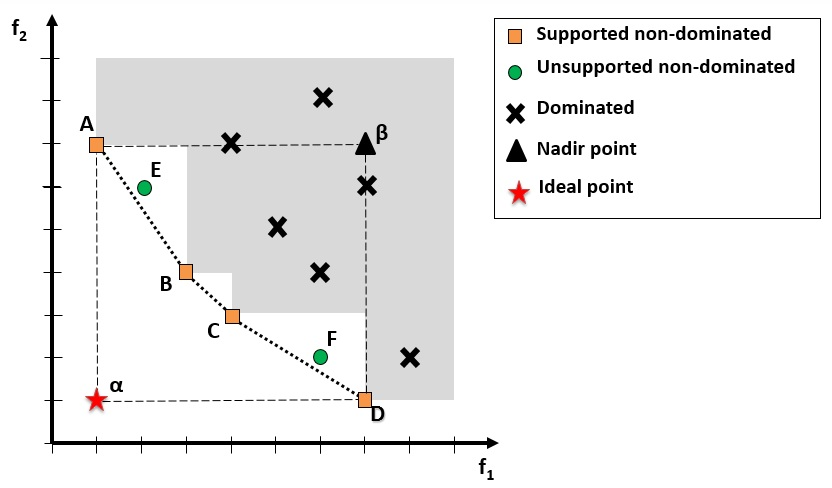
\includegraphics[width=1\textwidth]{Images/Chapter2/MOP-solutions}
\caption{Types of solutions and relevant points in a biobjective cost space.}
\label{fig:2-1}
\end{figure}

The Pareto-optimal solutions to the minimization problem can be split into two different types:
\begin{description}
    \item[Supported] They can be obtained as optimal solutions to a single-objective weighted sum problem (WSP). For instance, for the biobjective case (i.e. $q=2$), where $\vec x=(x_1,x_2)$, these include all optima of the following function, for all values of the $\lambda_1$ and $\lambda_2$ parameters.
\begin{equation}\label{chapMultiObjAlg:eq:wsp}
    \min_{x\in X} \lambda_1 x_1 + \lambda_2 x_2
\end{equation}
The set of all supported efficient solutions is denoted by $X_{S}$, and the set of non-dominated image values by $F_{S}$. 
    \item[Unsupported] The remaining non-dominated solutions are called \textit{unsupported} solutions. They cannot be obtained as solutions to WSPs. Unsupported solutions are located in the interior of triangles formed by two adjacent supported solutions. These areas are denominated \textit{duality gaps} by some authors. 
\end{description}

Let us take a look at Figure \ref{fig:2-1}, where a sample bidimensional image space is depicted. Points $A=(1,7)$, $B=(3,4)$, $C=(4,3)$,  and $D=(7,1)$ represent supported solutions. The \textit{extreme} non-dominated solutions are supported solutions that have the minimum possible value in at least one of the objectives (points $A$ and $D$). Points $E=(3,5)$ and $F=(6,2)$ represent unsupported non-dominated solutions. 

\begin{defi}\label{chapMultiObjAlg:def:nondom}
Given a set of vectors $X$, we shall define $\mathcal{N}(X)$ as the \textbf{set of non-dominated vectors} in $X$ in the following way:

\begin{equation}
  \mathcal{N}(X) = \{\vec x \in X \  | \  \nexists \vec y \in X \quad \vec y \prec \vec x\}
\end{equation}

\end{defi}

\begin{defi}
We say that a vector $\vec x$ is dominated by a set $X$ when 
there exists $\vec{x'}\in X$ such that $\vec{x'} \prec \vec x$. Thus, all points represented as crosses in Figure \ref{fig:2-1} are dominated by ${N}(X) = \{ (1,7) , (3,4), (4,3), (7,1) \}$.
\end{defi}

\begin{defi}\label{chapMultiObjAlg:def:idealnadir}
Let us denote $\alpha_i = min_{\vec x \in \mathcal{N}(X)}\{x_i\}$, and
$\beta_i = max_{\vec x \in \mathcal{N}(X)}\{x_i\}$. The set $\mathcal{N}(X)$ is bounded by the \textbf{ideal point} $\vec \alpha = (\alpha_1 \ldots \alpha_q)$,
and the anti-ideal or \textbf{nadir point} $\vec \beta = (\beta_1 \ldots \beta_q)$. The ideal point can be calculated optimizing each objective separately. However, for $q > 2$ it is difficult to calculate the nadir point without computing the whole set of non-dominated solutions. 
\end{defi}

In Figure \ref{fig:2-1} the ideal and nadir points are represented as a red star and a black triangle, respectively. The set $\mathcal{N}(X)$ is bounded by the extreme non-dominated solutions A and B, the ideal point ($\alpha$) and the nadir point ($\beta$).

Since there usually exist multiple Pareto-optimal solutions for Multiobjective Optimization Problems, there are different approaches in the literature to the concept of "solving a Multiobjective Optimization Problem". This concept is often understood as approximating or obtaining all or a representative set of Pareto-optimal solutions \citep{ehrgott2005}. Approaches can be also divided into those methods providing approximate solutions, and those providing exact solutions. 

There is a great variety of approximate techniques applied to the Multiobjective Optimization Problem e.g. fuzzy, and metaheuristics. Within them we can find a large amount of approaches like genetic algorithms, tabu search, or ant colony systems to name a few. A classification of all types of approaches to solve MOP is out the scope of this thesis. Some classifications can be found in \citep{Ehrgott2000,ehrgott2005,Branke2008}.   

Some popular exact approaches combine multiple objectives into one single objective. The most used one is the weighted sum or scalarization method. This method along with Multiobjective Linear Programming (MOLP) is often included within the exact algorithms, although only the set of supported solutions can be found. 

To classify exact algorithms that tackle the MOP we follow the general classification of MCDM methods, which can also be extended to MOP, proposed and followed by different authors over the years \citep{cohon1978,climacopascoal2012}. The following categories distinguish the methods according to the role of the decision maker in the resolution process: 

\begin{enumerate}
	\item \textbf{A priori methods}. The first category comprises those methods in which the preferences of the DM have been provided a priori. These preferences might be given for instance in the form of an utility function or goals to satisfy. Compromise Programming (CP) and Goal Programming (GP) are the most popular techniques included in this category. Some authors also believe than GP could be included in the next category \citep{Jones2010}, since it can be correctly used as a part of the interactive process to develop and refine the model accurately to reflect the decision maker preferences. 
	\item \textbf{Interactive decision process}. The decision maker can also be involved directly in the solution process. The methods which lie in this category establish a dialogue between the DM and the algorithmic resolution. If the DM is satisfied with the non-dominated solution provided, the algorithm finishes; otherwise, the calculation phase continues and the DM may set new preferences.
	\item \textbf{A posteriori methods}. The third category includes methods where a multiobjective analysis is performed. There are no preferences given by the decision maker and therefore, the whole set of efficient solutions must be calculated. Afterwards, this set is analyzed by the decision maker. It is worth mentioning that returning the whole Pareto frontier can be a computationally costly procedure. Therefore, these methods may have prohibitive runtimes when they are applied to large problems.
 
\end{enumerate}

The two mentioned a priori approaches are MCDM distance function methods. Actually, both methodological approaches aim to minimize the distance, not in a geometric sense but in a preferential one, between a certain point and the actual achievement for each of the objectives under consideration. This point is represented in GP as a set of targets. Analogously, CP uses the \emph{ideal point} (Definition \ref{chapMultiObjAlg:def:idealnadir}) which corresponds to the optimum value of each objective. 
%Finally, RPM represents this point as a reference level which plays the role of a control tool to be used in a mobile manner by the decision maker (DM) \citep{Romero1998}.

Let us now turn our attention to the Goal Programming methodology.

%-------------------------------------------------------------------
\section{Goal Programming}
\label{chapMultiObjAlg:sec:GP}
%-------------------------------------------------------------------

Goal programming is one of the oldest and most successful multicriteria decision making techniques \citep{ChankongHaimes1983}. GP was born in the beginning of the 1960s thanks to the contributions of \cite{Charnes1961}. Many variants and an impressive number of applications followed, enumerating hundreds of papers dealing with a wide range of problems and applications \citep{Ignizio1976, Ignizio1978, Ignizio1984, Charnes1977, Zeleny1981, Zeleny1982, Zeleny1984, Zanakis1985, Romero1986, Romero1991, Schniederjans1995, Tamiz1998, Aouni2001}. Several surveys have also been recently presented to review the improvements in the field \citep{Caballero2010,Orumie2014, Aouni2014}. 

Currently, GP has evolved from its original form into a powerful methodology that may incorporate techniques from artificial intelligence, such as genetic algorithms \citep{Pal2012, Deb1999} or fuzzy logic \citep{Bankian-Tabrizi2012, Shahnazari-Shahrezaei2013, Sen2013, DaSilva2014}. 
%or multicriteria search \citep{Mandow2001, Mandow2013, Pulido2014}.

Two key concepts serve to distinguish GP from conventional methods of optimization. First, the use of goals, or flexible constraints, as opposed to the rigid constraints of single objective optimization in mathematical programming, and second, the philosophy of ``satisficing'' as opposed to optimizing. The term satisfice was introduced by \citet{simon1956} as a combination of the terms satisfy and suffice. 

As a consequence of the principle of satisficing, any solution to a goal programming problem is ranked by an achievement function which measures the degree of deviation from the problem goals when these goals can not be satisfied. The specific way in which this deviation is measured characterizes the particular model of the GP approach that is employed.

It must be emphasized that, despite the popularity of the GP model, a weakness have been pointed out from the DM point of view. In general, GP methods do not guarantee that the obtained solution is Pareto-optimal, though some tests of Pareto optimality can be found in \citet{Miettinen1999, Larbani2007}. 
%This thesis is focused on the combination of the Multicriteria Search with goal-based preferences where all the algorithms proposed and analyzed in it return Pareto optimal solutions, regardless whether the goals can be satisfied or not. 

%-------------------------------------------------------------------
\subsection{Variants of goal-based preferences}
\label{chapMultiObjAlg:subsec:GP-variants}
%-------------------------------------------------------------------

Section \ref{chapMultiObjAlg:sec:MCDM} introduced the concepts of attribute, objective, target and deviation variables. Following those concepts, we introduce below the most popular GP formulation models. At this point, it is important to mention that inequalities have been traditionally used in mathematical programming models to define the set of feasible solutions to a problem. From a mathematical point of view, goals and constraints share the same syntax. However, their semantics are quite different. Constraints must be satisfied by candidate solutions to be acceptable. If all constraints cannot be simultaneously satisfied, the problem is inconsistent and there is no solution. Goals, on the other hand, are used to represent the decision maker's preferences. They represent their desires or aspirations. Hence, feasible solutions may or may not achieve all goals. A solution to a goal problem is \emph{satisfactory} when \emph{all} the goals can be satisfied. If there are no satisfactory solutions to a problem, GP seeks solutions that minimize deviation from the targets.

\cite{Romero1991} divides GP formulations in two categories. Both GP formulations do not generate the same solution, neither is one method superior to the other, because each variant is designed to satisfy certain decision makers' preferences. 

\begin{enumerate}

    \item \textbf{Weighted Goal Programming (WGP)}.
The first approach, called weighted goal programming (WGP), considers all goals simultaneously as they are all in a composite objective function. This function aims to minimize the sum of all the deviations between the goals and their aspirational levels. The deviations are weighted according to the relative importance of each goal for the DM.

In WGP weights are associated to each of the goals to establish the relative importance of deviations from their target. WGP handles several goals simultaneously by adding their relative deviations, hence, a normalization of constants is generally required in this model. Popular choices to normalize deviations are the goal target values (hence turning all deviations into percentages) or the range of the corresponding attribute (between the best and the worst possible values, hence mapping all deviations onto a zero-one range).

    \item \textbf{Lexicographic (or pre-emptive) Goal Programming (LGP)}.
The second approach, called pre-emptive or lexicographic goal programming (LGP), requires ranking all the goals in order of importance. The different goals are divided into several levels of pre-emptive priorities in such a way that if a specific priority level $Q_i$ is preferred to another priority level $Q_{i+1}$, then the fulfillment of the goals in $Q_i$ is infinitely more important than the fulfillment of the goals in $Q_{i+1}$. 

This variant models a problem with a combination of both weighted and lexicographic approaches. This model can suit the decision maker preferences when the attributes can be categorized into groups where the attributes within a group $k$ are infinitely more important to satisfy than those of level $k+1$. Each level can have one or more attributes and their importance within the level is established by a certain weight also defined by the DM. 
\end{enumerate}

We further analyze lexicographic goal-based preferences in the next section.

%-------------------------------------------------------------------
\subsection{Lexicographic goal-based preferences}
\label{chapMultiObjAlg:subsec:lex-MOP}
%-------------------------------------------------------------------

This section introduces a formal characterization of lexicographic goal-based preferences that will be later used in our formulation. Let us first recall that Goal Programming is a distance function method, that is, it aims to minimize the distance or deviation from the actual solution achievement to the point that represents the goals established by the DM. Therefore, the way to define and measure this deviation is an important component of the GP model. Let us now consider a problem, where goals are always of the form $g_i(\vec x) \leq t_i$. Let $\vec g = (g_1,g_2,...,g_q)$ be a vector of $1 \leq i \leq q$ attributes (costs) of a given solution $\vec x \in X$. Several methods have been proposed to measure the deviation of a solution vector from a set of goals. The most frequent ones are the following \citep{Romero1991, Romero1993}: 

\begin{itemize}
   \item minimization of the weighted sum of deviations: 
\begin{equation}\label{eq:deviation}
   d(\vec{g}) = \sum_{i=1}^{q} w_{i} \times \max(0, g_{i} - t_{i}), 
\end{equation}
	\item minimization of the maximum weighted deviation, also called minmax strategy:
\begin{equation}\label{eq:deviation-maxmin}
   d(\vec{g}) = \max_i[w_{i} \times \max(0, g_{i} - t_{i})].
\end{equation}
\end{itemize}

Notice that this definition measures the deviation of the vector $g$ with respect to the set of targets defined by the DM, i.e. corresponds to the aggregation of the non-achievement values of each individual goal $g_{i} - t_{i}$ (see Definition \ref{defi:deviation}). We do not consider deviation when a goal is satisfied. 

In the lexicographic goal-based model formulation we introduce below, we build upon the deviation measured as the minimization of the weighted sum of deviations. Let $\vec g = (g_1,g_2,...,g_q)$ be a vector of $1 \leq i \leq q$ attributes of a given solution $\vec x \in X$, where $g_i: X \rightarrow \mathbb{R}, 1 \leq i \leq q$ grouped in $l$ priority levels sorted in order of decreasing preemptive importance. Each priority level $k$ comprises a set $I_k$ of one or more attributes. Goals are defined by setting \emph{targets} $t_i$ for each attribute, always in the form $g_{i}(x) \leq t_{i}$.

This model considers the minimization of the weighted sum of deviations for each priority level, i.e. we measure the deviation of a solution vector from a set of goals grouped in preemptive priority levels of importance. We can calculate a deviation vector for $\vec g$ with one component for each priority level, $\vec{d}(\vec{g}) = (d_1(\vec{g}), d_2(\vec{g}),..., d_l(\vec{g}))$. For each level $k$, its deviation $d_k$ can be defined as:

\begin{equation}\label{eq:deviation-lex}
   d_k(\vec{g}) = \sum_{i\in I_k} w_{i} \times \max(0, g_{i} - t_{i})  
\end{equation}
where $w_i$ is the relative weight of goal $i$ in level $k$.

Let us now introduce some more relevant preference relations between vectors that will be employed throughout this research work.

\begin{defi}\label{chapMultiObjAlg:def:lexorder}
Let us consider two $q$-dimensional vectors $\vec y, \vec{y'} \in \mathbb{R}^q $. A total order relation $\prec_{L}$ denominated \textbf{lexicographic order} is defined as follows: 
\begin{equation}\label{chapMultiObjAlg:eq:lexorder}
 \vec{y} \prec_{L} \vec{y'} \ \ \Leftrightarrow \ \ \exists j \ (1\leq~i\leq~q) \ y_j < y'_j \ \land \ \forall i < j \ \ y_i = y'_i. 
\end{equation}
\end{defi}
and the preference relation $\preceq_{L}$: 
\begin{equation}
\forall \vec y,  \vec{y'} \in \mathbb{R}^q \quad \vec y \preceq_{L} \vec{y'} \ \ \Leftrightarrow \ \ 
\vec y \prec_{L} \vec{y'} \ \ \lor \ \ \vec y = \vec{y'}
\end{equation}

\begin{defi}\label{chapMultiObjAlg:def:linorder}
Let us consider two $q$-dimensional vectors $\vec y, \vec{y'} \in \mathbb{R}^q $. A total order relation $\prec_{lin}$ denominated \textbf{linear aggregation order} is defined as follows: 
\begin{equation}\label{chapMultiObjAlg:eq:linorder} \quad 
 \vec y \prec_{lin} \vec y' \ 
\Leftrightarrow \ \  
\sum_{i}{y_i} \ < \
\sum_{i}{y'_i} \ \ ,\ 1~\leq~i~\leq~q
\end{equation}
where $y_i$ denotes the i-th component of vector $\vec y$. 
\end{defi}

\begin{defi}\label{chapMultiObjAlg:def:weightedlinorder}
Let us consider two $q$-dimensional vectors $\vec y, \vec{y'} \in \mathbb{R}^q $. A total order relation $\prec_{wlin}$ denominated \textbf{weighted linear aggregation order} is defined as follows: 
\begin{equation}\label{chapMultiObjAlg:eq:weightedlinorder} \quad 
 \vec y \prec_{wlin} \vec y' \
\Leftrightarrow \ \ 
\sum_{i}{\lambda_i y_i} \ < \ 
\sum_{i}{\lambda_i y'_i} \ \ ,\ 1~\leq~i~\leq~q
\end{equation}
where $\vec \lambda$ stands for the vector of weights and $y_i,\lambda_i$ denote the i-th component of vectors $\vec y, \vec \lambda$. 
\end{defi}

A useful property of the previously mentioned orders (lexicographic, linear aggregation and weighted linear aggregation) is that their optimum in a set of vectors is also a non-dominated vector. 
%Thus, they are usually selected as ``tie-breaking'' rule by Multicriteria Search algorithms among non-dominated vectors. 
The order relations defined by $\prec_{L}$, $\prec_{lin}$ or $\prec_{wlin}$  are total orders. Then, given two different $q$-dimensional vectors $\vec y$ and $\vec{y'}$ (where $q > 1$), it is always possible to say that one is preferred to another. For instance, in a three-dimensional cost space there is no dominance relation between $(1,2,4)$ and $(3,2,1)$. However, $(1,2,4)\prec_{L} (3,2,1)$ and $(3,2,1) \prec_{lin} (1,2,4)$, since $3+2+1<1+2+4$. 


\begin{defi}\label{eq:optimum-achievement-vector}
We define the \textbf{optimum achievement} vector $\vec{d^*} = (d_1^*, d_2^*,..., d_l^*)$ as the minimum lexicographic deviation vector among all solutions. Thus, the set of 
%\textbf{goal-optimal} or 
satisfactory solutions consists of all feasible solutions with a deviation equal to $\vec{d^*}$. If there is at least a satisfactory solution, then the optimum achievement vector is equal to $\vec{0}$.
\end{defi}

Let us now address the issue of optimality. In general, GP methods do not guarantee that the obtained solution is Pareto-optimal or non-dominated. However, in this thesis we are concerned with methods or algorithms able to ensure that the solution to the GP model is also a non-dominated solution. Therefore, all the new algorithms devised and presented in this thesis lie in this category, defining a solution to the GP model as the set of all non-dominated solutions that satisfy the DM goals, or the set of non-dominated solutions that minimize the deviation from goals if these cannot be satisfied. 

Let us now define an order relation based on lexicographic goal preferences to guarantee our GP model only provides Pareto-optimal solutions,

\begin{defi}\label{chapMultiObjAlg:lexpreferences}
We define \textbf{lexicographic goal preferences} ($\prec_{G}$) as a partial order relation, 
\begin{equation} \label{eq:goalpref}
 \vec{y} \prec_{G} \vec{y'} \ \ \Leftrightarrow \ \ \vec{d}(\vec{y})
 \prec_{L} \vec{d}(\vec{y'}) \hspace{2 mm} \lor \hspace{2 mm}
 (\vec{d}(\vec{y}) = \vec{d}(\vec{y'}) \hspace{2 mm} \land \hspace{2
   mm} \vec{y} \prec \vec{y'})
\end{equation}

It is easy to see that  $\prec_{G}$ is a strict partial order (it is irreflexive and transitive). 
\end{defi}

\begin{defi}\label{chapMultiObjAlg:goaloptimalvectors}
Given a set of vectors $X$, we shall define $\mathcal{O}_G(X)$, the \textbf{set of optimal vectors} in $X$ \textbf{according to lexicographic goal preferences} (i.e. \emph{goal-optimal} vectors), as:

\begin{equation}\label{eq:goal-optimal-vectors}
  \mathcal{O}_G(X) = \{\vec x \in X \ \ | \ \ \nexists \vec y \in X \quad \vec{y} \prec_{G} \vec{x}\}
\end{equation}

Notice that an optimal solution according to $\prec_{G}$ is also a non-dominated solution, i.e. $\mathcal{O}_G(X) \subseteq \mathcal{N}(X)$.
\end{defi}

One of the main motivations of this thesis is the application of the GP approach to the Multicriteria Search Problem. In the next sections we introduce the Shortest Path Problem and its variant considering multiple objectives or criteria.

%-------------------------------------------------------------------
\section{The Shortest Path Problem}
\label{chapMultiObjAlg:sec:SPP}
%-------------------------------------------------------------------

The Shortest Path Problem (SPP) has been extensively studied for many years by the Artificial Intelligence (AI) and Operational Research (OR) communities, e.g. see \citep{Pearl1984, Gallo1988, Ahuja1990, Cherkassky1996}. In graph theory, the single-pair shortest path problem is the problem of finding a feasible path between two nodes (or vertices) such that the sum of the weights of its component arcs (or edges) is minimized. Finding the fastest route on a road map from one location to another is an example of the shortest path problem. In this case, the nodes represent locations and the arcs represent roads which are labeled with the cost to traverse them. 

Many real problems can be modeled as finding the shortest path between two nodes in a graph. Let us see a formal description of the problem.

Let $G =(N,A,c)$ be a locally finite labeled directed graph, defined by a set of
$N$ nodes, and a set of $A = \{ (i_i,j_1),...,(i_m,j_m) \} \subseteq N \times N$ arcs, where positive values $c_{ij} \in \mathbb{R}^{+}$ are associated with each arc $(i,j) \in A$. Sometimes we will denote $c_{ij}$ as $c(i,j)$.

\begin{defi}\label{chapMultiObjAlg:def:singleObjpath}
A \textbf{path} $P$  in $G$ is any sequence of nodes $P = (n_1, n_2,....n_k)$ such that $n_i \in N$ and for all $i < k$, $(n_i, n_{i+1}) \in A$. The set of all possible paths in $G$ is denoted by $\mathbb{P}$. 
\end{defi}

\begin{defi}\label{chapMultiObjAlg:def:singleObjcostpath}
The \textbf{cost of a path} $P$ is defined as the
sum of the costs of its component arcs,

\begin{equation}\label{chapMultiObjAlg:eq:singleObjaddCostPath}
    c(P) = \sum_{(i,j) \in P}{c(i,j)}
\end{equation}
\end{defi}

\begin{defi}\label{chapMultiObjAlg:def:singleObjSearchProb}
The \textbf{Shortest Path Problem} over a graph consists in finding the path $P\in \mathbb{P}$ in $G$ with the minimum cost $c(P)$ from a given a start node $s \in N$ to a destination\footnote{Graph search literature often refers to this node as the \emph{goal} node. However, in this research work we refer to it as destination node to avoid overloading the meaning of the word ``goal''. } node $t$. \footnote{In the literature SPP algorithms can be split into one-to-one and one-to-all, depending if they seek to find the optimal path to a given destination node or to all nodes in the graph. In this thesis, we are concerned with the one-to-one shortest path problem.}
\end{defi}

Shortest path algorithms can be classified in terms of different properties like the strategy used to explore the search graph, their admissibility, i.e. whether the returned solution is exact or approximate, or the use of distance estimates, among others. A complete classification and description of the different strategies can be found in \citet{korf2010}.

Most works on shortest path algorithms from the AI field distinguish two broad kinds of solution strategies:

\begin{description}
    \item[Best-first algorithms] 
%are based on the principle of optimality stated by \citet{bellman1954}. This principle applied to shortest path problems requires that an optimal path be made up of optimal subpaths. 
Best-first strategies are a general approach to solve graph search problems. Their main feature is selecting the best alternative at each step of the algorithm. Whenever several paths reach the same node, only the best one is preserved whereas the rest are discarded (or pruned). Although they are generally fast algorithms, their main drawback is that all promising alternatives must be kept in memory, which can easily exhaust memory resources for difficult problems.
	 \item[Depth-first algorithms] \citep{Korf1985} These strategies only consider the best next alternative, not keeping in memory other feasible alternatives which can be part of the optimal path. This leads to backtrack whenever the currently explored path cannot lead to a feasible solution. Depth-first strategies are specially suitable for tree problems and generally applied when the available memory resources are limited. 
\end{description}

Best-first search (BFS) algorithms generally expand the fewer nodes among all exact algorithms using the same cost function, but may require exponential space with solution depth. Depth-first search algorithms need space only linear in the maximum search depth, but generally expand more nodes than BFS. 

Dijkstra's algorithm \citep{dijkstra1959} is the most popular algorithm in this sense for one-to-one shortest path problems, i.e. finding the shortest path from a source node to a destination node in a graph. However, the reference algorithm in best-first search is \astar~ \citep{Hart1968}, which can be considered a generalization of Dijkstra's algorithm that uses \emph{heuristic knowledge}, or distance estimates, to focus the search on the most promising alternatives. 

The term \textit{heuristic} is employed by the \ac{AI} community to denote techniques that exploit knowledge about the problem to improve their efficiency. On the other hand, the \ac{OR} community uses the term heuristic to denote methods used to speed up the process of finding good approximate solutions. In order to avoid confusion, algorithms that may return exact solutions like \astar \ are frequently categorized as ``heuristic search'' in the AI literature. In this research work we refer to the terms ``heuristic function'' or ``heuristic estimates'' used in the context of \astar-like algorithms simply as ``distance estimates''.  

As stated above, the main feature of best-first algorithms is selecting at each step of the algorithm the most promising node $n$ according to a certain evaluation function. Let $g(n)$ denote the accrued cost of a path from $s$, the source node, to $n$. Dijkstra's algorithm uses $g(n)$ as the evaluation function, i.e. it selects the node with the lowest value of $g(n)$ to scan next. The \astar~ algorithm uses distance estimates to predict how close is the evaluated node to the destination node. This function is denoted by $h(n)$. Thus, the evaluation function employed by \astar~ is $f(n) = g(n) + h(n)$. 

Best-first algorithms keep all the recorded alternative paths with source in $s$ stored in a search tree. Efficient selection of the current best candidate for expansion is typically implemented using a priority queue ordered by the evaluation function. Each alternative path is labeled with the cost of the path, and additionally a reference to the parent node to recover the solution path at the end of the algorithm. The labels still pending to be explored are typically stored in a queue of $OPEN$ alternatives. A distinct set of $CLOSED$ nodes can be used to store already evaluated alternatives, in order to perform duplicate detection. 

\begin{defi}\label{chapMultiObjAlg:def:singleObjlabel}
A \textbf{node label} stands for the cost of a path found to a given node. In single-objective algorithms each node $n$ is labeled with a single value, that stands for the cost of the current best known path to $n$. 
\end{defi}

At each step the label of some node $n_i$ is selected and scanned (or expanded), and all the possible extensions via outgoing arcs of node $n_i$ are generated and compared with actual stored labels in successor nodes. The stored cost for an adjacent node $n_j$ is updated whenever the extension of the selected path through some outgoing arc of $n_i$ represent a least cost path to the node $n_j$.

In the OR literature, shortest path algorithms are frequently classified as \textbf{label-setting} or \textbf{label-correcting}. For example, Dijkstra's algorithm \citep{dijkstra1959} is label-setting, since every extended path becomes permanent. This path represents the least cost to the node, i.e. once an alternative is scanned and extended, it is guaranteed that the least cost path to this node has already been found. In label-correcting algorithms, e.g. see \citep{zhannoon2000}, this is not guaranteed until all nodes have been examined, since the label of an already explored node can be corrected by a new better one.

Label-setting algorithms repeat an iterative node labeling process until the destination node is selected for extension\footnote{We refer to the one-to-one version of Dijkstra's algorithm. In the one-to-all version, the algorithm will not finish until all nodes have been visited.}. Then, the optimal cost of the path is found in the node label. The actual optimal path can be recovered tracing back pointers to parents.

In Dijkstra's algorithm, any permanent node label stands for the optimal shortest path distance from $s$ to the node. Therefore, a ``closed'' node will never be re-opened. In the case of \astar, a permanent label may store the optimal path or not depending on properties related to the distance estimate function $h(n)$. Hence, let us now review the formal properties of $h(n)$ relevant to \astar. 

\begin{defi}\label{chapMultiObjAlg:def:singleObjoptimistic}
Let $h^*(n)$ be the actual optimal cost of a path from $n$ to a destination node $t$. A distance estimate function $h(n)$ is \textbf{optimistic} when
\begin{equation}\label{chapMultiObjAlg:eq:singleObjoptimistic}
 h(n) \leq h^*(n) \quad \forall n \in N 
\end{equation}
\end{defi}

\begin{defi}\label{chapMultiObjAlg:def:singleObjConsistency}
Let $k(n,n')$ denote the cost of an optimal path in $G$ from a node $n$ to another node $n'$. A distance estimate function $h(n)$ is \textbf{consistent} when 
\begin{equation}\label{chapMultiObjAlg:eq:singleObjConsistency}
 h(n) + k(n,n') \leq h(n') \quad \forall n,n' \in N 
\end{equation}
\end{defi}

\begin{defi}\label{chapMultiObjAlg:def:singleObjMonotonicity}
Equivalently, a distance estimate function $h(n)$ is said to be \textbf{monotone} when
\begin{equation}\label{chapMultiObjAlg:eq:singleObjMonotonicity}
 h(n) + c(n,n') \leq h(n') \quad \forall (n,n') \in A 
\end{equation}
\end{defi}

\begin{defi}\label{chapMultiObjAlg:def:singleObjMoreInformedHeu}
A distance estimate function $h_2(n)$ is said to be \textbf{more informed} than another distance estimate function $h_1(n)$ when both are optimistic and
\begin{equation}\label{chapMultiObjAlg:eq:singleObjMoreInformedHeu}
 h_2(n) > h_1(n) \quad \forall n \in N, n \neq t 
\end{equation}
\end{defi}

There is a strong relationship between the properties of $h(n)$ and the efficiency and quality of results produced by \astar~, e.g. see \citep{Pearl1984}.

\begin{property}[Admissibility]\label{chapMultiObjAlg:eq:singleObjAdmissibility}

On finite graphs, when $h(n)$ is a lower bound of the cost of an optimal path from $n$ to $t$ (i.e., it is optimistic) \astar \ is \textbf{admissible}, i.e. \textbf{it is guaranteed to find an optimal solution if this solution exists, i.e. it is an exact algorithm}. \astar~ is \emph{admissible} even on infinite graphs with some additional assumptions:
\begin{eqnarray}\label{chapMultiObjAlg:eq:singleObjAdmissibilityCond}
\forall n \in N,\ h(n) \geq 0   \newline \\    
\nonumber \forall (n,n') \in A,\ c(n,n') \geq \epsilon > 0  
\end{eqnarray}
\end{property}

\begin{property}[Efficiency]\label{chapMultiObjAlg:eq:singleObjEfficiency}

When $\forall n \in N, \  h(n) = 0$, \astar~ is equivalent to the one-to-one version of Dijkstra's algorithm. When $h(n)$ is \textbf{consistent} or \textbf{monotone}, \astar~ is a label-setting algorithm, and requires, in the worst case $O(|N|)$ iterations, storing $O(|N|)$ nodes in memory. If the cost of the optimal solution is denoted by $c^*=k(s,t)$, \astar~ will always expand for sure all labels with $f(n) < c^*$. For those with $f(n) = c^*$, only those belonging to the returned optimal solution path will be necessarily expanded. Given an optimistic distance estimate function, more actual suboptimal alternatives can be pushed out the search frontier $f(n) = c^*$ with \textbf{more informed} functions, i.e. bigger values of $h(n)$, reducing search effort.
\end{property}

\begin{property}[Optimality]\label{chapMultiObjAlg:eq:singleObjOptimality}

When the distance estimate function $h(n)$ is \textbf{monotone}, 
%the cost of a path found by the algorithm is known to be optimal and it is not necessary to re-open nodes (a permanent node will not come back to $OPEN$). Moreover, 
\astar~ is  proven to be \textbf{optimal} among the class of admissible best-first algorithms\footnote{Defined as the class of single-pair unidirectional search algorithms.} \citep{Dechterpearl1985}, in the number of scanned nodes to find the solution. In other words, any node scanned by \astar~ must be also scanned by another algorithm in this class to preserve admissibility.
\end{property}
 
%-------------------------------------------------------------------
\section{The Multicriteria Search Problem}
\label{chapMultiObjAlg:sec:MSP}
%-------------------------------------------------------------------

The problem of finding a shortest path from a source node to a destination node has been considered, traditionally, as a single-objective optimization problem. However, real decision problems frequently involve multiple conflicting criteria. Therefore, it seems natural to extend the SPP to the multicriteria case. Multicriteria preferences over paths in a graph can be expressed in the same ways already analyzed in the previous sections. For example, the solution to the Multiobjective Search Problem is the set of the so-called Pareto-optimal solution paths. This was in fact the first Multicriteria Search Problem to be analyzed by \citet{hansen1979}. Multicriteria Search Problems have a wide range of practical applications in different domains, arising naturally in many fields, such as:

\begin{itemize}
	\item \textbf{Robot surveillance} \citep{dellefaveetal2009}. The problem consists in how to automate surveillance tasks based on robotic platforms and fixed sensors. This surveillance automation is a complex problem posing many technical challenges, where robots must find a path to visit a set of locations equipped with alarms.
	\item \textbf{Transportation of hazardous materials}. The problem is concerned with finding routes with minimum cost and minimum risk \citep{Erkut2007,caramiaetal2010,Machucaetal2011}. 
	\item \textbf{Satellite scheduling}. \citet{Gabrel2002} proposed the problem of scheduling an Earth Observing Satellite as a Multicriteria Search Problem. A label-correcting was presented to take into consideration three objectives: demand satisfaction of shots taken by the satellite, priority of those shots (related to strategic importance), and satellite use (related to the number of instruments on/off). 
	\item \textbf{Robot path planning}. The problem consists in finding a navigation path for a mobile robot that must consider multiple costs in navigation, such as the length of the path, traversability of the area, time to travel to the destination location, etc. \citep{Fujimura1996}. A similar problem deals with autonomous aerial vehicles and involves the motion planning that consists of a sequence of connected linear tracks (or trajectory segments) \citep{Wu2011}.
	\item \textbf{Route planning in different contexts}. In a road network problem several parameters (such as time, distance, economical cost, etc.) can be considered either the problem takes into account a single vehicle or a fleet \citep{Jozefowiez2008,Delling2009,Machuca2012}.
	\item \textbf{Public transportation}. Multicriteria problems over an urban transportation network consider the minimization of the overall cost, time and users' discomfort \citep{Modesti1998}. \citet{Raith2009} presented the cyclist route choice as a new application of the bi-objective shortest path problem where cyclists aim to reach their destination in minimal travel time, but also along a safe route. Multicriteria search on time dependent public transportation systems is another application recently studied \citep{Wu2004,Muller-Hannemann2004,Pyrga2008,Disser2008}. These problems usually involve the minimization of travel time, bus-train changes, walking distance, etc. 
	\item \textbf{QoS in networks}. In these problems the criteria to minimize may be, for example, number of lost packages, maximal delay time of packages, traffic crossing by a link, route length, probability of route unreliability, etc. \citep{climacoetal2003, craveirinha2009}.
\end{itemize}

We will introduce some useful definitions before presenting a formal definition of the Multiobjective Shortest Path Problem. Let $G =(N,A,\vec c)$ be a locally finite labeled directed graph, defined by a set of $N$ nodes, and a set $A = \{ (i_i,j_1),...,(i_m,j_m) \} \subseteq N \times N$ of arcs, where $q$ positive costs $\vec c_{ij} = (c^1_{ij},..., c^q_{ij}) \in \mathbb{R}^{q+}$ are associated with each arc $(i,j) \in A$. Sometimes we will denote $\vec c_{ij}$ as $\vec c(i,j)$.

Let a path in $G$ be any sequence of nodes $P = (n_1, n_2,....n_k)$ such that for all $i < k$, $(n_i, n_{i+1}) \in A$. A problem over a multicriteria graph is defined by a start node $s \in N$, and a destination node $t$. Each path in the graph of the form $P = (s,..., n_i,n_{i+1},...,t)$ represents a feasible solution to the problem. 

\begin{defi}\label{chapMultiObjAlg:def:multiObjcostpath}
The \textbf{cost of a path} $P$ in multiobjective shortest path problems is a $q$-dimensional vector defined as the sum of the costs of its arcs,

\begin{equation}\label{chapMultiObjAlg:eq:multiObjaddCostPath}
    \vec c(P) = \sum_{(i,j) \in P}{\vec c(i,j)} 
\end{equation}
\end{defi}

\begin{defi}\label{chapMultiObjAlg:def:multiObjsolution}
Given a start node $s \in N$ and a destination node $t \in N$, the Multiobjective Shortest Path Problem consists in finding all the non-dominated paths from $s$ to $t$. More precisely, the problem can be formulated mathematically as the following network flow problem [adapted from \cite{Raith2009a}]
\end{defi}

\begin{eqnarray}
min \quad \vec f(x) =  \left\lbrace
  \begin{array}{l}
     f_1(x) = \displaystyle\sum_{(i,j) \in A}{c^1_{ij} x_{ij}}, \\
     ... \\
     f_q(x) = \displaystyle\sum_{(i,j) \in A}{c^q_{ij} x_{ij}}, \\
  \end{array}
  \right.
\end{eqnarray}
\begin{eqnarray}
\label{eq:form-constraints}
s.t. \quad \displaystyle\sum_{(i,j) \in A}{x_{ij}} \quad - \quad \displaystyle\sum_{(j,i) \in A}{x_{ji}} =  \left\lbrace
  \begin{array}{l}
     1 \qquad \text{if } \ i = s, \\
     0 \qquad \text{if } \ i\neq s,t, \\
     -1 \quad \ \text{if } \ i = t \\
  \end{array}
  \right.
\end{eqnarray}
\begin{eqnarray}
x_{ij} \in \{0,1\}, \quad \text{for all} \ (i,j) \in A.  
\end{eqnarray}
where $x$ is a vector of flows on the arcs, and the constraints (\ref{eq:form-constraints}) represent flow balance at the different nodes.

As stated above, many problems from a wide variety of fields can be formulated as Multicriteria Search Problems. There are not less algorithmic approaches to cope with these problems. As explained in Section \ref{chapMultiObjAlg:sec:MOP}, algorithmic approaches to this problem can be divided into exact and approximate. 

Multicriteria Search Problems are indeed a particular case of the MCDM problems, hence, the classification presented in Section \ref{chapMultiObjAlg:sec:MOP} for the MOP can also be extended to them. A detailed description of all types of approaches to solve MSP is out the scope of this thesis. Some classifications can be found in \citet{Ehrgott2000,ehrgott2005,Tarapata2007,climacopascoal2012}.  

Let us now review some of the exact algorithms that have been proposed to deal with MSP categorized according to the role of the decision maker. We omit the interactive methods described in Section \ref{chapMultiObjAlg:sec:MOP}, since they are out of the scope of this thesis. Some proposed methods can be found in \citet{Current1990,Granat2003}.

First, we will review with some detail exact algorithms with a posteriori preferences. These are used when no a priori preferential information is available. Basically, these algorithms find the set of all Pareto-optimal solutions to the problem, so that the most preferred ones can be selected a posteriori. We will pay special attention to the \namoa \ search algorithm, which uses lower bound estimates to efficiently find the set of all Pareto-optimal paths to a problem. On the contrary, a priori algorithms have preferential information from the decision maker. These may be expressed, for example, in the form of a set of goals. A basic approach to solve this problem is to use a posteriori algorithms, and then select the preferred ones among them. However, sometimes it is also possible to devise algorithms that find only the preferred alternatives. In this thesis, we will analyze both approaches in the solution of the shortest path problem with lexicographic goal preferences.

%-------------------------------------------------------------------
\section{Exact a posteriori algorithms}
\label{chapMultiObjAlg:sec:a-posteriori}
%-------------------------------------------------------------------

Four categories of exact algorithms without a priori preferences from the DM have been identified by different authors \citep{skriverandersen2000,Raith2009,climacopascoal2012,Machuca2012a}. Three of them are generalizations from single-objective shortest path problems, these are label-setting, label-correcting and k-th shortest paths; the last one is a two-phase approach.

A \textbf{label} (or node label) stands for the cost of a path found from the start to a given node. In single-objective search, a node $n$ is labeled with a single value that stands for the cost of the current best known path to $n$. In multiobjective search algorithms, multiple non-dominated paths can reach a node $n$, therefore, $n$ is not labeled with a single cost but with a set of node labels which stand for the non-dominated cost vectors of known paths that reach node $n$.

\begin{description}

    \item[Label-setting methods] The most classical single-objective shortest path algorithms follow a labeling method. Their name derives from the process of labeling each node with the cost of the best path found so far to reach that node. The multiobjective label-setting algorithms follow the same strategy, with the necessary adaptations to the multicriteria case. An iterative process scans alternatives and generates new successors until the stopping criterion is fulfilled. Then, the labels at the destination node represent efficient costs of solution paths. The first proposals of multicriteria label-setting algorithms can be found in \citep{hansen1979,Martins1984a}. 
    
    Another interesting field of study for label-setting algorithms is to reduce space requirements, e.g. frontier search algorithms \citep{Korf2005}, which have also been extended to the multicriteria case \citep{Mandow2007, Mandow2008, Mandow2008a}.
    
    \item[Label-correcting methods] The main difference between label-correcting and label-setting algorithms is the label selection policy. Label-setting algorithms employ a best-first strategy whereas that label-correcting algorithms follow different strategies, e.g. FIFO. This different strategy does not allow these algorithms to guarantee that any label selected for expansion is optimal, therefore if a better path to some node is found the suboptimal labels will be ``corrected'' by the new one. An analysis of multicriteria label-correcting methods can be found in \citep{Brumbaugh-Smith1989}. Some analysis which compare label-correcting and label-setting approaches appear in \citep{skriverandersen2000, guerrieromusmanno2001, Paixao2007}.
       
    \item[Ranking methods] In a similar manner to k-best single-objective algorithms, multiobjective ranking algorithms employ a ranking method to list paths by a non-decreasing total order. However, there exist two necessary adaptations in these algorithms. First, an order must be imposed to rank solutions either using a linear combination of the objectives, or a partial order (e.g. lexicographic order). Second, the algorithm can not be stopped until all efficient solutions are guaranteed to be found. Moreover, the value of $k$ is unknown a priori. 
    
    A complete literature review of ranking algorithms applied to the MSP can be found in \citep{martinsetal2007,climacopascoal2012}. Some ranking algorithms appear in \citep{martins1984c,azevedomartins1991,martinsetal2007,paixaosantos2008}. Several recent studies, however, have found  these algorithms not competitive with label-setting and label-correcting methods \citep{huarngetal1996,skriverandersen2000,Raith2009}.
    
    \item[Two-phase methods] Algorithms from this category compute the extreme supported efficient solutions in a first phase. In a second phase the remaining unsupported efficient solutions are calculated with a labeling algorithm. Depending on the method chosen for the first phase an initialization phase may be necessary. They have been applied to the Bicriteria Search Problem (BSP) by \citet{Mote1991,Raith2009a,Raith2009}. However, they have been found to be generally slower than the label-setting or label-correcting algorithms \citep{Raith2009a,Raith2009}.
    
\end{description}

In labeling search algorithms two different successor generation strategies have been applied, \textit{node-selection} and \textit{label-selection}. The \textit{node-selection} strategy implies that all labels belonging to a node are expanded simultaneously, on the contrary, if only one label at a time is expanded it is called \textit{label-selection}. 

%-------------------------------------------------------------------
\subsection{Extensions of \texorpdfstring{\astar}{A*} to the multiobjective case}
\label{chapMultiObjAlg:subsec:label-setting}
%-------------------------------------------------------------------

Several extensions of \astar \ to the Multiobjective case have been proposed. The behavior of these algorithms does not easily fit in the usual OR categories, and depends largely on the properties of the distance estimate. \citet{hansen1979} presented a bi-objective extension of Dijkstra's label setting algorithm. \citet{Martins1984} proposed a general label-setting algorithm for the multiobjective case. \citet{stewartwhite1991} proposed a multiobjective algorithm based on node-selection, called \moa (Multiobjective \astar). \citet{Tung1992} proposed two multicriteria lower bound functions along with a label-setting multicriteria algorithm. \citet{Mandow2010} presented \namoa (A New Approach to Multiobjective \astar), a multiobjective algorithm that has been proven to be an exact algorithm when provided with lower bound estimates, and to explore an optimal number of labels.

Recent works studied the influence of lower bounds on multicriteria search algorithms. The thesis of \citet{Machuca2012a} evaluated the algorithms of Tung \& Chew, \moa, and \namoa \ with and without lower bound estimates. The main outcome obtained was the improvement, in general, of \namoa \ when provided with lower bounds, and its formal and empirical superiority over the other two algorithms when provided with lower bounds  \citep[2.4.3]{Machuca2012a}. A formal explanation for the superiority of \namoa \ over \moa \ was presented recently by \citet{PerezdelaCruz2013}. This paper considers the performance of \moa \ when provided with lower bounds, and analyzes a pathological behavior observed in \moa, namely, that the efficiency of the algorithm decreases with more informed distance estimates. It is shown that in certain cases uninformed search is more efficient for \moa \ than perfectly informed search, in terms of both node and label expansions. Thus, we consider \moa \ obsolete and we will focus our attention in \namoa.

We present \namoa \ below, and we will further analyze the use of the ideal point as a multicriteria lower bound function. This was proposed by Tung and Chew and we will apply it to \namoa.

%-------------------------------------------------------------------
\subsection{Algorithm \texorpdfstring{\namoa}{NAMOA*}}
\label{chapMultiObjAlg:subsec:namoa}
%-------------------------------------------------------------------

\namoa \ \citep{Mandow2005,Mandow2010} is a successful generalization of \astar \ to the multiobjective case. \namoa \ is defined to accept a lower bound function $H(n)$ that returns a set of cost estimates of all non-dominated paths from node $n$ to a node which belongs to a set of destination nodes. Table \ref{ChapMultiObjAlg:tab:pseudocode-namoa} shows the pseudocode of \namoa \ simplified to use a single vector estimate $\vec h(n)$ and one destination node $t$. 

\namoa \ is a best-first algorithm that uses a \textit{label-selection} strategy and builds a search graph $SG$ rooted at the start node $s$ to store all non-dominated paths found to each node. The set COSTS stores all known non-dominated solution costs to the destination node $t$. Each node $n$ in the search graph has two sets of labels: $G_{op}(n)$ denotes the set of cost vectors of paths reaching $n$ that can be further explored, while $G_{cl}(n)$ denotes the set of those that have already been expanded (in fact COSTS is equivalent to $G_{cl}(t)$) and we refer to them as closed or permanent (when the lower bound function satisfies certain conditions). Each cost vector in these sets labels one or more arcs in the graph from $n$ to its parents. \namoa \ uses extended labels $(n, \vec g, \vec f)$. By abuse of language, we refer to them as labels when there is no ambiguity. 

Let $ \vec g(P_{sn})$ be the cost of some path $P_{sn}$ reaching some node $n$ from the start node. Then, $\vec h(n)$ is a lower bound of the cost of any extension of such path to the destination node and $\vec f(P_{sn}) =  \vec g(P_{sn}) +  \vec h(n)$ the evaluation function used.

\begin{table}
\caption{[Adapted from \citep{Mandow2010}] Pseudocode of $\text{NAMOA}^*$ algorithm.}
\scalebox{.95}{
\begin{tabular}{p{\columnwidth}}
\hline
\begin{enumerate}
\item CREATE:
  \par --- An empty search graph SG, and place $s$ as its root.
  \par --- Two sets $G_{cl}(s) = \emptyset$ and $G_{op}(s)=
  \{(\vec{0})\}$.   
  \par --- A list of alternatives, OPEN = $\{(s, \vec{0}, \vec h(s)\} $.
  \par --- An empty set, COSTS.

\item \label{label-selection} PATH SELECTION. If OPEN is not empty, then, 

  \par --- Select a label $(n, \vec g_n, \vec f_n) $ from
  OPEN (``PATH SELECTION STRATEGY'') \newline  such that $\nexists (n', \vec g_{n'}, \vec f_{n'}) \in$ OPEN $ \ \ | \ \ \vec f_{n'} \prec \vec f_n$.

  \par --- Delete the selected label from OPEN, and move $\vec g_n$ from $G_{op}(n)$ to $G_{cl}(n)$. 
  
  \par --- If \ $\exists \vec{c^*} \in$ COSTS $\ \ | \ \ \vec{c^*} \prec
  \vec f_n$, then repeat step \ref{label-selection}  (lazy filtering)
  
\item CHECK TERMINATION. If OPEN is empty, then backtrack in SG from $t$ and return the set of solution paths with costs in COSTS.

\item SOLUTION RECORDING. If $n$ is the destination node, then
    \par --- Include $\vec g_n$ in COSTS.
    \par --- Go back to step \ref{label-selection}.

\item PATH EXPANSION: If $n$ is not the destination node, then for all successor nodes $m$ of $n$ do:
  \begin{enumerate}
    \item Calculate the cost of the new path found to $m$ and its
     lower bound, $\vec g_m = \vec g_n + \vec c(n,m)$,  $\vec f_m = \vec g(m) + \vec h(m)$.
    \item If $\nexists \vec{c^*} \in$ COSTS $\ \ | \ \ \vec{c^*} \prec \vec f_m$, (``FILTERING'') then: \label{chapMultiObjAlg:alg:filteringNamoa}
      \begin{enumerate}
      \item If $m \notin$ SG: 
	\begin{itemize}
	\item Set $G_{op}(m)= \{(\vec g_m)\}$ and add $(m, \vec g_m, \vec f_m)$ to OPEN.
	\item Label with $\vec g_m$ a pointer from $n$ to $m$.
	\end{itemize}
      \item else if $\vec g_m$ equals some cost vector in  $G_{op}(m) \cup G_{cl}(m)$ then
	\begin{itemize}
	\item Label with $\vec g_m$ a pointer from $n$ to $m$.
	\end{itemize}
      \item  else if $\vec f_m$ is not dominated by $G_{cl}(m) \cup G_{op}(m)$ (``PRUNING''), then:  
	\begin{itemize}
   \item Eliminate vectors $\vec g_{m'} \in G_{op}(m) \ \ |
          \ \ \vec g_m \prec \vec g_{m'}$ and its corresponding label $(m, \vec g_{m'}, \vec f_{m'})$ from OPEN.
	\item Add $(m, \vec g_m, \vec f_m)$ to OPEN,
          $\vec g_m$ to $G_{op}(m)$ and label with $\vec g_m$ a
          pointer from $n$ to $m$.
	\end{itemize}
      \end{enumerate}
    \item Go back to step \ref{label-selection}.
  \end{enumerate}
\end{enumerate}
\\ \hline
\end{tabular}
}
\label{ChapMultiObjAlg:tab:pseudocode-namoa} 
\end{table}

At each iteration, a label with a non-dominated $\vec f$ in OPEN is selected for expansion. If $n$ is the destination node, then $\vec f$ is stored in COSTS, the set of non-dominated solutions costs. Otherwise, the non-dominated label $(n, \vec g,  \vec f)$ selected from OPEN is made permanent (i.e., $ g$ is moved from $G_{op}(n)$ to $G_{cl}(n)$). For each arc in the graph $(n, n')$ with cost $ \vec c(n, n')$, a new label is generated for node $n'$ with cost $\vec{g'} = \vec  g + \vec  c(n, n')$. Several operations are carried out in \namoa \ for each such label:

\begin{enumerate}
	\item The algorithm applies the optimality principle, i.e. only non-dominated labels to each node are considered. Therefore, the new label has to be checked for dominance against all labels in $G_{op}(n)$ and $G_{cl}(n)$. If the new label is dominated, then it is discarded. This operation is called \emph{pruning}.
	\item For each new label, its cost estimate $\vec{f'} = \vec{g'} + \vec  h(n')$ is tested for dominance against vectors in COSTS. If the new estimate is dominated, it can never lead to a new non-dominated solution and is discarded. This operation is called \emph{filtering}.
\end{enumerate}

These operations are computationally costly. For the case with two objectives the label sets $G_{op}(n), G_{cl}(n)$ and COSTS can be ordered lexicographically, allowing for efficient dominance checks \citep{SandersMandow2013}. However, for three or more objectives there is no known efficient way to check the dominance of a vector against a set. 

A difference between the original pseudocode and this adaptation in Table \ref{ChapMultiObjAlg:tab:pseudocode-namoa} is the application of \textit{lazy filtering}, as described in \citep{SandersMandow2013}, i.e. we do not explicitly filter existing labels when a new solution is found. Labels are tested and, if necessary, filtered only after selection. This prevents a costly update operation.

\namoa \ shares important properties with A$^*$. If the estimate function $\vec h(n)$ returns an optimistic estimate (lower bound) of the cost of \emph{any} path from $n$ to the destination, then it is guaranteed to terminate with the set of all non-dominated solution paths to the problem. If the lower bound function satisfies the so-called monotone property, then it explores only non-dominated labels and is optimal in the class of admissible algorithms, see Section \ref{chapFormalAnalysis:sec:analysisNAMOA} for further details. 

%-------------------------------------------------------------------
\subsection{The ideal point as lower bound}
\label{chapMultiObjAlg:subsec:tc}
%-------------------------------------------------------------------

The use of lower bound functions has been studied for many years as a way to improve the efficiency of combinatorial optimization problem solving. In graph search problems a lower bound function estimates the cost of a solution path from node $n$ to the destination node $t$. In MSP there is more than one criterion, therefore, this function does not return a single value but a cost vector estimate. \citet{Tung1992} proposed a multicriteria lower bound function along with a label-setting multicriteria algorithm. The lower bound function represents the ideal point presented in Definition \ref{chapMultiObjAlg:def:idealnadir}. This is indeed the most informed and admissible estimate function that can be defined for a MSP\footnote{\citet{Tung1992} called this lower bound $\vec q(n,n')$.} and we will name it as $\vec h_\alpha$.

The lower bound function is defined as $\vec h_\alpha (n)=(c_1^*(n), c_2^*(n), \ldots c_q^*(n))$, where $c_i^*(n)$ is the optimal scalar cost of a path from $n$ to the destination node, considering only the \textit{i-th} cost component. These values are precalculated by reversing all arcs in the graph, originally labeled with cost vector $\vec c(n,n') = (c_1, c_2,\ldots c_q)$ the new labels will be of the form $c_i(n',n) = c_i$. Any single-objective one-to-all shortest path problem can be applied to find the optimal cost from the destination node to all the other nodes in the reversed graph. This process will be executed $q$ times, once for each scalar cost. Ties are broken by a lexicographic order, taking into account the other cost components.

The method proposed by Tung and Chew to calculate the $\vec h_\alpha$ function considered originally the estimation for all nodes in the graph. In medium and difficult multiobjective problems this precalculation time is minor in comparison with the runtime of the multiobjective algorithm. However, this time can be proportionally significant when the destination node is ``close'' to the source node. \citet{Machuca2011b} presented a bounded calculation procedure for this lower bound function in bicriteria problems that avoids calculating the estimate for all nodes in the graph. They also compared the performance of \namoa \ over road map problems with three different lower bound functions, the corrected great circle distance, the distance estimate $\vec h_\alpha$, and bounded $\vec h_\alpha$. The latter clearly outperformed the other two. 

Let us now review the equivalent formal properties of multicriteria lower bound functions $H(n)$ to the single-valued function. These properties can be briefly review in \citep[2.1.2.1]{Machuca2012a} or in-depth in \citep{Pearl1984}. 

\begin{defi}\label{chapFormalAnalysis:def:multiObjadmissibleH}
\citep[p. 184]{Mandow2005}
A distance estimate function $H(n)$ is said to be admissible when for all non-dominated solutions $P^*=(s=n_0, n_1, \ldots,n_i,$ $n_{i+1},\ldots,n_l=t)$, and for all subpaths $P_{i}^*=(n_0,\ldots,n_i)$ of $P^*$ the following holds:

\begin{equation}\label{chapFormalAnalysis:eq:multiObjadmissibleH}
\exists \vec h \in H(n_i) \quad | \quad g(P_i^*) + \vec h \preceq g(P^*)
\end{equation}
\end{defi}

\begin{defi}\label{chapFormalAnalysis:def:multiObjconsistentH}
\citep[Definition 5.6]{Mandow2010}
  A multicriteria lower bound function $H(n)$ is \textbf{consistent} if for all pairs of nodes $n, n'$ in the graph, for all non-dominated path between them $P=(n,\ldots,n')$, and for all lower bound cost vectors $\vec h' \in H(n')$, the following condition holds:
\begin{equation}
\exists \vec h \in H(n) \quad | \quad \vec h \preceq c(P) + \vec{h'}  
\end{equation}

\end{defi}

\begin{defi}\label{chapFormalAnalysis:def:multiObjmonotoneH}
\citep[Definition 5.7]{Mandow2010} 
  Equivalently, a multicriteria lower bound function $H(n)$ is \textbf{monotone} when for all arcs $(n, n')$ in the graph, the following condition holds:
\begin{equation}
\forall \vec{h'} \in H(n') \quad \exists \vec h \in H(n) \quad | \quad \vec h \preceq c(n,n') + \vec{h'} 
\end{equation}
\end{defi}

\begin{defi}\label{chapFormalAnalysis:def:multiObjmoreinformedH}
\citep[Definition 5.4]{Mandow2010} A multicriteria lower bound function $H_2(n)$ is said to be \textbf{at least as informed} as other $H_1(n)$ when both are admissible and for all nodes $n$,
\begin{equation}
\forall \vec h_2 \in H_2(n) \quad \exists \vec h_1 \in H_1(n) \quad | \quad \vec h_1 \preceq \vec h_2
\end{equation}
\end{defi}

%-------------------------------------------------------------------
\section{Exact a priori algorithms}
\label{chapMultiObjAlg:sec:a-priori}
%-------------------------------------------------------------------

Finally, we will review relevant exact multicriteria algorithms proposed for the case where preferences between alternatives are provided a priori. More precisely, we review the cases where preferences are expressed in terms of compromise solutions, or a set of goals. Both of these a priori techniques aim to minimize the distance between the DM preferences and the actual achievement for each of the objectives under consideration.

%-------------------------------------------------------------------
\subsection{Compromise Search}
\label{chapMultiObjAlg:subsec:compromise}
%-------------------------------------------------------------------

A well known approach in MSP is the compromise solution method \citep{Yu1985} or best compromise search. In this case, the preferences of the DM can be given as their aspiration level on each criterion. Then, a function is defined to evaluate a solution according to its distance to that preference, which is called the reference point. The best compromise solution is then the closest one to the reference point\footnote{The reference point does not need to be necessarily specified by the DM and it can also be defined as the ideal solution point \citep{Zeleny1982}. In this case, this approach could be included in the a posteriori category.}.

Achievement scalarizing functions are employed in Compromise Search in order to evaluate solutions. Let us take the following definition from \citep{Machuca2013}: 

\begin{defi}\label{def:scalarizing-function}
A scalarizing function $s$ must have the following properties: (1) any non-dominated solution can be optimal with respect to s (with an appropriate choice of parameters); and (2) any optimal solution with respect to s has to be non-dominated. These requirements ensure that, for any rational decision maker, the preferred solution can be reached optimizing some scalarizing function. 
\end{defi}

The Tchebycheff norm, the Euclidean, Manhattan or Minkowski's are examples of distance functions to seek for the compromise search solution. However, there does not exist any scalarizing function satisfying simultaneously the two requirements \citep{Wierzbicki1986}. Even so, Compromise Search applied to MSP has been widely studied, and compared to algorithms where the whole set of non-dominated solutions is returned \citep{Machuca2013}.  

\citet{Perny2005} introduced a general formalism for preference-based combinatorial problems, and proposed several algorithms to obtain the set of preferred solutions. Different measures are used in best compromise search to obtain the set of compromise solutions. The ordered weighted averaging (OWA) operator is a natural manner to express the preferences between solutions. \citet{galandspanjaard2007} proposed a best compromise search algorithm based on OWA, called OWA$^*$. \citet{Galand2010} used the Choquet integral, another preference model used in decision theory for aggregating preferences, as a preference model. The Tchebycheff scalarizing function was employed by other recent studies as \citet{Perny2010} and \citet{Galand2013}. The latter, presented the first bidirectional multiobjective search algorithm, called bidirectional PBMOA$^*$.  

\citet{Galand2006} presented two algorithms to find the best compromise solution paths, BCA$^*$ and kA$^*$. BCA$^*$ is a variant of \namoa \ with an upper bound $\lambda$ to store the value of the Tchebychev distance of the best compromise solution path found. Additionally, the algorithm incorporates a specific stopping condition. In the worst case, BCA$^*$ performs a similar enumeration of paths as \namoa, and finds the best compromise at the last step. On average, however, BCA$^*$ stops much earlier than \namoa. kA$^*$ enumerates the $k$ best paths in a scalarized version of the multiobjective graph. This algorithm relies on a modified version of \astar \ that works on labels attached to paths instead of labels attached to nodes. 

Several differences between both algorithms can be pointed out. First, the use of vectors versus scalar values in BCA$^*$ and kA$^*$, respectively. Second, BCA$^*$ prunes sub-optimal paths reaching the same node as well as those paths that according to their $\vec f$ value cannot lead to the best compromise solutions. kA$^*$, however, cannot prune sub-optimal paths, since they should always be kept for future considerations. Finally, the comparison between both algorithms revealed a better performance of kA$^*$ in certain cases \citep{Galand2006,Machuca2013}. Nevertheless, kA$^*$ presents an exponential worst case behavior, i.e. it can explicitly explore a combinatorially large number of paths with the same cost vector. 

Lastly, \citet{Sauvanet2010} presented two improvements to speed-up the search of BCA$^*$, applying that development to a bicycle routing application available online and for smartphones\footnote{Website: \url{www.geovelo.fr, Android APP: https://play.google.com/store/apps/details?id=fr.geoveloparis}}.

%-------------------------------------------------------------------
\subsection{Goal Programming}
\label{chapMultiObjAlg:subsec:goal-programming}
%-------------------------------------------------------------------

Goal Programming has also been applied to the MSP. Different approaches to model a GP problem were presented in Section \ref{chapMultiObjAlg:subsec:GP-variants}. One of them is Lexicographic Goal Programming. \metal \citep{Mandow2001} was proposed as a general algorithm for graph search problems with additive lexicographic goals. In a way, it is an extension of \astar \ to goal-based multicriteria preferences.

Section \ref{chapMultiObjAlg:subsec:label-setting} analyzed the proposed extensions of \astar \ to the multiobjective case. As we stated there, \moa \ is considered obsolete due to the formal and empirical superiority of \namoa \ over \moa. \metal \ is based on \moa, and subject also to the same faults detected in the work of \citet{PerezdelaCruz2013} for \moa, namely, that the performance of the algorithm decreases with better informed distance estimates. Therefore, this algorithm can also be considered deprecated, and will not be further considered in this research work. To our knowledge, there have been no further developments on MSP with Lexicographic Goals. This thesis addresses precisely this question. In Chapter \ref{chapContributions} we will present two new algorithms based on \namoa \ to deal with lexicographic goals. 

%-------------------------------------------------------------------
\section{Summary and motivation}
\label{chapMultiObjAlg:sec:summary}
%-------------------------------------------------------------------

In this chapter we have reviewed the fundamental concepts of Multicriteria Decision Theory, with special attention to goal-based preferences. We have also reviewed the Multicriteria Shortest Path Problem and the main approaches proposed to date in the literature to solve it. All methods developed in this chapter have been mainly divided into approximate and exact techniques. In this thesis we focus on exact algorithmic techniques, i.e. those techniques seeking only non-dominated solutions, either the full set of the Pareto frontier, or the subset of Pareto-optimal solutions that satisfy the DM preferences. 

Four categories of exact a posteriori algorithms were identified in Section \ref{chapMultiObjAlg:sec:a-posteriori}: labeling (label-setting
and label-correcting), ranking, and two phases approaches. This thesis focuses on label-setting algorithms using lower bound estimates. We pay special attention to the Dijkstra and \astar \ algorithmic extensions to the Multiobjective case. In particular, we describe an improved dominance check method for \namoa.

Among a priori methods, we reviewed contributions in Compromise Search and Goal Based Search. Formulations for the WGP and the Lexicographic GP were presented. To our knowledge, the only previous work on goal-based preferences for SPP was based on \moa, and there are no contributions in this sense based on \namoa. We will further describe in this thesis our contributions in the category of label-setting algorithms with lower bounds that employ a label-selection policy, and lexicographic goal programming algorithmic techniques. In particular,
one of the main contributions of this thesis relies on an extension of \namoa \ to deal with lexicographic goal techniques. In those cases where the goals cannot be satisfied the distance to the goals is measured with the definition stated in \ref{eq:deviation}, which minimizes the weighted sum of deviations. Table \ref{tab:summary-algorithms} displays a classification of representative a priori and a posteriori multicriteria shortest path algorithms with additive metrics.

\begin{sidewaystable}
\caption{Classification of some representative a priori and a posteriori multicriteria shortest path algorithms.}
\centering
\begin{tabular}{llllll}
\hline \noalign{\smallskip}
\multicolumn{5}{c}{Classification} & Some representative algorithms \\
\noalign{\smallskip} \hline \noalign{\smallskip}
\multirow{6}{*}{\rotatebox[origin=c]{90}{A posteriori}} & \multirow{4}{*}{Labeling} &  \multirow{3}{*}{Label-setting} & \multicolumn{2}{l}{MO Dijkstra } & \citet{hansen1979,Martins1984} \\ 
 & & & \multirow{2}{*}{MO \astar} & \emph{Node-selection} & \moa \\
 & & & & \emph{Label-selection} & \citet{Tung1992}; \namoa; Vector frontier Search \\
 & & \multicolumn{3}{l}{Label correcting} & \citet{Brumbaugh-Smith1989,guerrieromusmanno2001} \\
 & \multicolumn{4}{l}{Ranking} & %\citet{climacomartins1981, 
\citet{martinsetal2007,paixaosantos2008} \\
  & \multicolumn{4}{l}{Two phases} & \citet{Mote1991,Raith2009a} \\
\noalign{\smallskip} \hline \noalign{\smallskip}
\multirow{4}{*}{\rotatebox[origin=c]{90}{A priori}} & \multirow{4}{*}{CP} & \multicolumn{3}{l}{Tchebycheff norm} & BCA$^*$, kA$^*$; \citet{Sauvanet2010} \\
 & & \multicolumn{3}{l}{OWA operator} & OWA$^*$, Bidirectional PBMOA$^*$ \\ %\citet{galandspanjaard2007} \\
 & & \multicolumn{3}{l}{Choquet integral} & \citet{Galand2010} \\
% & & \multicolumn{3}{l}{Bidirectional} &  \\ %\citet{Galand2013} \\
 & GP & \multicolumn{3}{l}{LGP} & \metal \\
\noalign{\smallskip} 
\hline
\end{tabular}
\label{tab:summary-algorithms}
\end{sidewaystable}  

This thesis aims to provide a contribution to the Multicriteria Search Problems with lexicographic goal-based preferences. In other words, the combination of the MSP with GP techniques. We define two alternatives to deal with such a problem. The first alternative approaches the problem from the perspective of an optimization problem. A full search of the Pareto frontier is performed to obtain all the non-dominated solutions, and afterwards extract the subset of satisfactory solutions for the provided goals. The second alternative approaches the problem from the satisfaction perspective. An algorithm which takes advantage of the preferences given by the DM is devised. Its purpose is to restrict the search and discard sooner in the search those paths which will not lead to satisfactory solutions. The first alternative is characterized as a posteriori method, while the second corresponds to the category of a priori methods. 

In addition to define a new specifically designed algorithm to cope with MSP with lexicographic goal-based preferences (second alternative presented above), we aim to improve the runtime performance of algorithms based on the extension of \astar \ to the multiobjective case (label-setting algorithms within the first alternative). More specifically, we will apply the devised techniques to \namoa. 

Time requirements have been identified as the limiting factor in the size of problems that can be practically solved by multiobjective shortest path algorithms \citep{Machuca2009, Machuca2012, Mali2012}. Thus, we enumerate below several fundamental aspects to achieve better runtime performance in label-setting algorithms.

\begin{enumerate}
	\item \textbf{Use of lower bounds.} In the same manner than A$^*$ outperforms Dijkstra's algorithm by using lower bounds, or estimates of the distance to the destination node, the label-setting multicriteria search algorithms can also take advantage of these bounds to discard sooner suboptimal paths and ``guide'' the search more efficiently. Recent studies have demonstrated that \textit{node-selection} algorithms as \moa \ does not share all the formal properties of A$^*$. However, \namoa \ following a \textit{label-selection} strategy does preserve all formal properties of A$^*$ \citep{Mandow2010}, see Section \ref{chapFormalAnalysis:sec:analysisNAMOA}. 
	
    \item \textbf{More efficient dominance checks.} Several adaptations are necessary to generalize algorithms to the multicriteria case. The most important factor to consider is the fact that a set of non-dominated labels need to be kept at a node, instead of a single label as in the single-objective case. Therefore, a great amount of dominance checks will be necessary to check if a new generated path must be discarded\footnote{For bi-objective cases labels can be totally ordered by using the lexicographic order, reducing time requirements to determine whether a new label is non-dominated with existing labels, for instance, with a lexicographic order all labels in the set are sorted by the first objective, hence, a single comparison of the second objective of the new label and the best value for any label in the set will be enough to check the dominance of the new label against the whole set. However, for the general MSP case, all labels must be compared against the new one to check whether is dominated or not.}. Thus, we propose in this thesis a new dimensionality reduction technique to speed up dominance checks in label-setting multicriteria search algorithms, see Section \ref{chapMultiObjAlg:sec:Time-efficient-MSalg}.
	
	\item \textbf{Label selection policy in best-first algorithms.} Best-first algorithms employ a selection policy to choose between all non-dominated alternatives. We presented several total order relations in Section \ref{chapMultiObjAlg:subsec:lex-MOP} which can be used as label selection policies, being the lexicographic and linear addition orders the most commonly used. Different studies have been made to compare the performance of label-setting algorithms employing these orders \citep{Iori2010, Machuca2012}. In the experiments presented in this thesis, label selection policies are also analyzed as an important parameter in the algorithm time performance.
	
	\item \textbf{Use of more efficient data structures.} The use of efficient data structures for the SPP has always been a hot topic \citep{Ahuja1990,Zhan1997,Cherkassky1999,Cazenave2006,Mehlhorn2007}. Nevertheless, the use of different data structures to sort the list of open alternatives in best-first MSP still deserves more research. We will further analyze this and other future improvements in Chapter \ref{ChapConclusions}.  
\end{enumerate}

%---------------------------------------------------------------------
%
% Chapter 3: Benchmarks
%
%---------------------------------------------------------------------
%
% ChapMultiObjTestBeds.tex
% Copyright 2015 Dr. Francisco J. Pulido
%
% This file belongs to the PhD titled "New Techniques and Algorithms for Multiobjective and Lexicographic Goal-Based Shortest Path Problems", distributed under the Creative Commons Licence Attribution-NonCommercial-NoDerivs 3.0, available in http://creativecommons.org/licenses/by-nc-nd/3.0/. The complete PhD dissertation is freely accessible from http://www.lcc.uma.es/~francis/
%
% This thesis has been written adapting the TeXiS template, a LaTeX template for writting thesis and other documents. The complete TeXiS package can be obtained from http://gaia.fdi.ucm.es/projects/texis/. TeXis is distributed under the same conditions of the LaTeX Project Public License (http://www.latex-project.org/lppl.txt). The complete license is available in http://creativecommons.org/licenses/by-sa/3.0/legalcode
%
%---------------------------------------------------------------------

\chapter{Benchmarks}
\label{chapMultiObjTestBeds}
%
\begin{FraseCelebre}
\begin{Frase}
A goal is not always meant to be reached, it often serves simply as something to aim at.
\end{Frase}
\begin{Fuente}
Bruce Lee (1940-1973)
\end{Fuente}
\end{FraseCelebre}

This chapter introduces relevant literature on the experimental evaluation of multiobjective search algorithms and describes the test sets used to assess the performance of the algorithms studied in this thesis. We survey some of the tools and test beds proposed in the past to test algorithmic improvements in the field, review the importance of connecting the theoretical analysis with empirical evaluation, and enumerate important factors to consider in the latter.

The chapter is organized as follows. First, a summary of related benchmarks and previous test sets used by authors on Multiobjective Search can be found in Section \ref{chapMultiObjTestBeds:sec:Antecedents}. Section \ref{chapMultiObjTestBeds:sec:Benchmarks} describes artificial and realistic scenarios employed to test the algorithms presented in this thesis. Section \ref{chapMultiObjTestBeds:sec:Performance} addresses the different factors involved in the evaluation of performance from two points of view: what variables must be measured and what implementation and external factors are desirable to control.
 
%-------------------------------------------------------------------
\section{Multiobjective Search benchmarks}
\label{chapMultiObjTestBeds:sec:Antecedents}
%-------------------------------------------------------------------

The empirical evaluation of algorithms is a main tool of research in Computer Science \citep{johnson2002}. Theoretical studies can provide formal proofs of correctness and indicate the superiority of one algorithm over another, however, the point of research is, and has always been, applying those algorithms to real life problems. To do so, an empirical evaluation, either on simulated or realistic scenarios, is needed to confirm the results already provided in a theoretical manner. Wherever formal studies can not be provided, an empirical evaluation is the best way to approach the problem.

An empirical evaluation is based on two principles. First, reproducibility, i.e. guaranteeing that other researchers may obtain equivalent results when they use the same parameters to reproduce the experiments; and second, fairness, i.e. algorithms should share as much code as possible, define clearly implementation and execution parameters, as well as employ benchmarks or problems available online, see for example the 9th DIMACS Implementation challenge described below.

In this thesis we tackle the Multicriteria Search Problem and consider goals provided by a decision maker that define the subset of Pareto optimal solutions to be returned. On one hand, Multicriteria Search performance can be related to a number of distinct factors relative to the benchmark, such as graph size and shape, number of arcs, solution depth, costs range, number of criteria or correlation between objectives. On the other hand, Goal Programming is also concerned with the efficiency, which can be attributed to the form that the preferences are given, as well as the amount of solutions that satisfy them.
%Goal Programming methods are more concerned to model the problem as realistically as possible. Hence, they focus on providing satisfactory solutions to the decision maker. Thus, we aim to model the decision maker preferences and employ benchmarks to measure the performance of algorithms which can solve that problem. 
Therefore, we define our empirical evaluation based on parameters relative to the graph, problem, and preferences given by the DM. 

Many test beds have been proposed over the years for Multiobjective Search problems, for instance, randomly generated graphs, grids or road maps, see Section 3.1 \citep{Machuca2012a} for a recent survey of the literature in Multiobjective Search benchmarks. For instance, \citet{klingmanetal1974} published NETGEN, a random graph generator that first generates a connected skeleton and then adds arcs randomly. \citet{skriverandersen2000} used this tool in their research, however, they presented a new random graph generator, NETMAKER, arguing that graphs generated with NETGEN only had a small number of efficient solutions, even for large scale graphs. 

In order to generate graphs, NETMAKER needs two input parameters: the branching factor and the interval length. The latter specifies which nodes are allowed to be reached from a particular node. Other random graphs have been proposed over the years \citep{hansen1979,JoaoCarlosNamoradoClimaco1982,nanceetal1987,Brumbaugh-Smith1989, Mote1991, gandibleuxetal2006,martinsetal2007,Iori2010,caramiaetal2010,Galand2010}.

Euclidean, rectangular, and square grids are another alternative to test multiobjective search algorithms performance. They have also been extensively used in the literature, e.g.  \citep{Mote1991,guerrieromusmanno2001,guerrieroetal2001,martinsetal2007,caramiaetal2010}.
% A Euclidean graph is a graph in which the vertices represent points in the plane, and the edges are assigned lengths equal to the Euclidean distance between those points; while a planar graph is a graph that can be embedded in the plane, i.e., it can be drawn on the plane in such a way that its edges intersect only at their endpoints. 

Several road maps scenarios have been provided for experimentation purposes, like the 9th DIMACS implementation challenge, see Section \ref{chapMultiObjTestBeds:subsec:RoadMaps} for further details, maps obtained from OpenStreetMap~\footnote{\url{http://www.openstreetmap.org/}} \citep{Raith2009a,Raith2009}, road networks from the Italian region of Lazio \citep{caramiaetal2010}, or small maps of Auckland (New Zealand) \citep{Raith2009} for the bi-objective cyclist route problem. 

To our knowledge, there are no specific benchmarks developed to test goal-based graph search algorithms.

%-------------------------------------------------------------------
\section{Benchmarks used in this thesis}
\label{chapMultiObjTestBeds:sec:Benchmarks}
%-------------------------------------------------------------------

A combination of artificial and realistic scenarios are used in this thesis to assess the performance of the proposed algorithms. Artificially generated environments, like random grids, allow to control different parameters, such as number of nodes, branching factor, correlation between objectives or solution depth. Therefore, these are suitable to analyze tendencies over increasingly difficult problem instances. 

On the other hand, realistic scenarios come with a fixed set of parameters, which can not be modified at will. However, these provide first-hand information on the applicability of the proposed algorithms. 

The evaluation strategy in this thesis combines both artificial and realistic scenarios. First, we test the performance over artificially designed environments, and then over realistic scenarios.

In addition to these scenarios, we aim to evaluate the performance of Multicriteria Search Problems according to different preferences, or sets of goals grouped in priority levels. Thus, we propose several classes of targets that emulate the possible preferences of a decision maker. These targets split the experiments into two classes of problems (see Section \ref{chapEmpiricalAnalysis:sec:grids} for a detailed description of the experimental setup). Thus, we analyze the efficiency: (1) according to the satisfiability of the goals (whether they can be satisfied or not) (2) when goals can be satisfied; the size of the set of efficient solutions with respect to the size of the Pareto set. Let us now review the benchmarks.

%-------------------------------------------------------------------
\subsection{Random grids}
\label{chapMultiObjTestBeds:subsec:RandomGrids}
%-------------------------------------------------------------------

Artificially generated graphs and grids are the most extensively test sets used in the literature. In order to adequate the problem difficulty in graphs, several parameters have to be defined, such as branching factor, number of arcs, and mainly, the topology of the graph. Square grids have a fixed vicinity, are easy to create, and their size can be gradually increased.  

Grids can also be considered a realistic scenario compatible with real-file applications, e.g. pathfinding in computer games \citep{bayilipolat2011}. Moreover, a recent study from \citet{paixaosantos2008} revealed that problems defined over randomly generated graphs have a number of non-dominated solutions larger than graphs with similar configurations.

The random grids used in this thesis are designed to allow the controlled evaluation of performance with respect to solution depth. In particular, we have generated square bi-dimensional grids of $100 \times 100$, bidirectional arcs and a vicinity of four neighbors, i.e. grids with 10,000 nodes and 39,800 arcs. The start node is placed at the grid center $(50,50)$ and a single destination node is placed in the diagonal from the center to the bottom right corner. 

Different solution depths are considered, varying from 20 to 100, i.e. for solution depth $d$, the destination node is at coordinates $(50 + d/2, 50 + d/2)$. A set of five different problems is generated for each solution depth. For each arc $q$ integer scalar costs $\vec c(i,j) = (c_1,c_2,...,c_q)$ are randomly generated in the range [1,10] using an uniform distribution, i.e. leading to uncorrelated objectives. Table \ref{tab:3-1} shows the average number of Pareto-optimal solutions for each solution depth and number of objectives considered in our random grids experiments. 

\begin{table}
\caption{Average number of Pareto-optimal cost vectors relative to solution depth and number of objectives ($q$) in our grid problems.}
\centering
\scalebox{1}{
\begin{tabular}{crr}
\hline \noalign{\smallskip}
$q$ & Sol. depth & Avg. |C$^*$| \\
\noalign{\smallskip} \hline
3 & 20 & 122 \\
3 & 30 & 302 \\
3 & 40 & 694 \\
3 & 50 & 1,599 \\
3 & 60 & 2,007 \\
3 & 70 & 2,561 \\
3 & 80 & 5,423 \\
3 & 90 & 5,912 \\
3 & 100 & 8,307 \\
\hline 
\noalign{\smallskip} 
4 & 20 & 493 \\
4 & 30 & 2,230 \\
4 & 40 & 7,826  \\
4 & 50 & 24,942 \\
\hline
\noalign{\smallskip}  
5 & 20 & 1,819 \\
5 & 30 & 10,830 \\
5 & 40 & 49,634 \\
\hline
\end{tabular}
}
\label{tab:3-1}
\end{table}

%-------------------------------------------------------------------
\subsection{Road maps}
\label{chapMultiObjTestBeds:subsec:RoadMaps}
%-------------------------------------------------------------------

Among the multiple realistic domains where Multicriteria Search arises (see Section \ref{chapMultiObjAlg:sec:MSP} for a detailed classification of several application domains for MSP) we have selected route planing. Route planing is currently a hot research topic driven partly by the boom of GPS navigation devices and on-line route planners.

Single-objective search on road maps has been intensively studied over the last decades \citep{Pearl1984,Zhan1998a,Klunder2006,Geisberger2008,schultes2008,Delling2009a}. However, research on multiobjective route planning is a recent area of interest \citep{Delling2009,Raith2009a,Machuca2011,Machuca2011b, Mali2012} and it is expected to become even more popular with the progressive introduction of electrical vehicles \citep{Baum2014, Goodrich2014} to optimize the trade-off between attributes like energy consumption or travel time. 

The experiments presented in this thesis involve the use of realistic road maps from the 9th DIMACS Implementation Challenge: Shortest Path. Road maps are defined as graphs where arcs represent roads and nodes represent road junctions. Coordinates (longitude and latitude) are also provided for each node. The test bed comprises a set of twelve road maps of increasing size\footnote{\url{http://www.dis.uniroma1.it/challenge9/}}. These data were provided by the 2000 U.S. Census Bureau's TIGER/Line R database (Topologically Integrated Geographic Encoding and Referencing system). 

The original DIMACS maps provide two different criteria: physical distance and travel time. An additional criterion was introduced in \citet{Machuca2011} by estimating economic cost. This was obtained combining certain values for tolls and fuel consumption according to road category. The resulting values are not linearly correlated to those of the other cost values. The experiments reported in Chapter \ref{chapEmpiricalAnalysisRoadMaps} consider the simultaneous minimization of these three attributes, physical distance $(c_1)$, travel time $(c_2)$, and economic cost $(c_3)$.  

\citet{Machuca2011b} generated fifty problem instances for each of the four smallest maps from the DIMACS Challenge: New York, San Francisco Bay Area, Colorado and Florida, to minimize simultaneously attributes $(c_1)$ and $(c_2)$. Given that our experimental evaluation considers the minimization of three attributes instead of two, our problems have much higher difficulty and therefore, we only selected the first twenty problems of the New York city map. Additionally, due to the fact that only fourteen out of the twenty problems of New York could be solved within the runtime limit, we employed a second road map from the Vermont State\footnote{Available on \url{http://www.dis.uniroma1.it/challenge9/data/tiger/}} and generated twenty random problems in a similar way. The Vermont State road map represents an interesting benchmark to observe performance trends, since all algorithms solve all problem instances within the runtime limit. 

%-------------------------------------------------------------------
\subsection{Significance of the test sets}
\label{chapMultiObjTestBeds:sec:significanceGrids}
%-------------------------------------------------------------------

Regarding random grid problems, the majority of past studies focus on the bi-criterion case \citep{Raith2009, Machuca2012a}. Among those considering the multicriteria case, \citet{caramiaetal2010} use grids of $20 \times 20$ nodes and 167.5 efficient paths in average, \citet{martinsetal2007,Paixao2007} also use grids with $20 \times 20$ nodes but a greater number of efficient paths, since they generated arcs cost in the range [1,1000]). Our experimental test on Multicriteria Search consider in general larger instances than those studies.

Regarding road map experiments, \citet{Machuca2012a} presented recent experiments over two sets of problems: 
\begin{enumerate}
	\item A first set of problems minimizes \textit{distance} ($c_1$) and \textit{time} ($c_2$) values provided by the DIMACS challenge maps.
	\item A second set of problems minimizes \textit{time} ($c_2$) and \textit{economic cost} ($c_3$). 	
\end{enumerate}

Table \ref{tab:3-2} illustrates the average number of Pareto-optimal solutions for each set of our problems. Pearson's correlation coefficient for costs $c_1$ and $c_2$ is 0.96 while that for $c_2$ and $c_3$ is 0.16, i.e. there is a strong linear correlation between time and distance, while there is no such a correlation between travel time and economic cost. 

The sets of experiments with two objectives proposed by \citet{Machuca2012a} were composed by 50 problem instances, while our test set with three objectives comprises only twenty instances. We decided to reduce the number of problems in the test set due to the greater difficulty of the three objectives search compared to the bi-objective. Table \ref{tab:3-2} shows the average number of Pareto-optimal solution vectors for experiments with ($c_1$,$c_2$), ($c_2$,$c_3$), and ($c_1,c_2,c_3$) cost functions. For New York city road map, the average number of Pareto-optimal solution vectors of ($c_1,c_2,c_3$) experiments shows an asterisk. This indicates that 47,738.8 represents the average considering only the fourteen solvable problems of the set. Yet this number is approximately 240 and 22 times greater than the average Pareto-optimal solution vectors in experiments with ($c_1$,$c_2$) and ($c_2$,$c_3$) cost functions, respectively. In consequence, we expect our test sets to be in line with the hardest ones proposed to date for multiobjective search.

\begin{table}
    \caption{Average Pareto-optimal cost vectors for three sets of experiments. ($^+$) represents the average of the fourteen problems solved.}
    \begin{minipage}{.5\linewidth}
      \centering
        \begin{tabular}{lr}
			\hline \noalign{\smallskip}
			\multicolumn{2}{c}{New York city road map} \\
			\noalign{\smallskip} 
			Set of problems & Average |C$^*$| \\
			\noalign{\smallskip} \hline
			($c_1,c_2$) & 198.6 \\
			($c_2,c_3$) & 2,086.6 \\
			($c_1,c_2,c_3$) & $^+$47,738.8 \\
			\hline
			\end{tabular}
    \end{minipage}%
    \begin{minipage}{.5\linewidth}
      \centering
			\begin{tabular}{lr}
			\hline \noalign{\smallskip}
			\multicolumn{2}{c}{Vermont road map} \\
			\noalign{\smallskip}
			Set of problems & Average |C$^*$| \\
			\noalign{\smallskip} \hline
			($c_1,c_2$) & 81.6 \\
			($c_2,c_3$) & 247.1 \\
			($c_1,c_2,c_3$) & 3,334.6 \\
			\hline
			\end{tabular}
		\label{tab:3-2}
    \end{minipage} 
\end{table}

%-------------------------------------------------------------------
\subsection{Evaluation of preferences based on goals}
\label{chapMultiObjTestBeds:subsec:Performance}
%-------------------------------------------------------------------

In order to assess the impact of the goals satisfiability on the efficiency of the goal-based algorithms, we employ a lexicographic goal programming model that considers three goals grouped in two priority levels: \\
 
Level 1 \hspace{10 mm} $g_1 \leq t_1, \hspace{5 mm} w_{1} = 0.5$ \\
\hphantom{a} \hspace{26 mm} $g_2 \leq t_2, \hspace{5 mm} w_{2} = 0.5$ 

Level 2 \hspace{10 mm} $g_3 \leq t_3, \hspace{5 mm} w_{3} = 1$ \\

Sets of target values for each problem are defined in terms of the ideal  $\vec \alpha = (\alpha_1, \alpha_2, \alpha_3)$, and  nadir points  $\vec \beta = (\beta_1, \beta_2, \beta_3)$. These were previously calculated from the full Pareto sets obtained with \namoa. The nadir point is generally unknown in practice, but we take advantage of it in these experiments to obtain targets with different degrees of satisfaction for the purpose of experimentation. In a practical situation the ideal point is known thanks to the lower bound precalculations \citep{Tung1992}. These also provide the nadir point for two objectives, and at least an approximation for three or more objectives.

Two different classes of experiments were carried out. For the first class, five different target sets were calculated as follows: 
\begin{equation} \label{eq:targets}
t_i = \alpha_i + (\beta_i - \alpha_i) \times k_1, \qquad k_1 \in \{ 0, 0.25, 0.5, 0.75, 1 \}  
\end{equation}

For example, for $k_1=1$ all Pareto-optimal solutions will satisfy all goals, and for $k_1=0$ no Pareto solution will likely satisfy them. 

For the second class, targets of the first level were fixed for $k_1=0.75$ and $k_1=0.5$, which were found to provide satisfactory solutions. We then measured efficiency setting stricter targets for the third goal:
\begin{equation} \label{eq:targets2}
t_3 = \alpha_3 + (\beta_3 - \alpha_3) \times k_2 \qquad k_2 = k_1 \times k^\prime, \quad \textrm{where} \ k^\prime \in \{ 0.25, 0.5, 0.75, 1 \}  
\end{equation}. 

These values of $t_3$ allow us to evaluate the performance when some goals are satisfied and some not. 

%-------------------------------------------------------------------
\section{Evaluation of performance in Multicriteria Search}
\label{chapMultiObjTestBeds:sec:Performance}
%-------------------------------------------------------------------

In the following chapters we introduce three new algorithms. The first one, called \lexgo, is a goal-based algorithm; the second one, \namoate, represents a specialization of \namoa, and the last, \lexgote, is devised as a specialization of \lexgo. We use these algorithms to evaluate two alternatives to deal with MSP with goal preferences. In the first one, \namoa \ and \namoate \ return the full Pareto set of non-dominated solutions to the problem and determine the subset of solutions that satisfy the goals from that set. In the second one, \lexgo \ and \lexgote \ are used to search only for goal-optimal solutions. 

Our purpose with these new algorithms can be summarized with two statements. In the first place, improve the performance of both alternatives, and in the second place, assess their performance.

This evaluation of the performance is usually characterized with respect to solution depth, explored labels, correlation between objectives \citep{Brumbaugh-Smith1989,Mote1991,Machuca2010} or the presence/absence of lower bounds.

All proposed algorithms are based on \namoa.
%(although the t-discarding technique, presented in Section \ref{chapMultiObjAlg:sec:Time-efficient-MSalg}, is applicable to any Multicriteria Search labeling algorithm)
It has been proved that the more informed a consistent lower bound function is, the smaller the number of labels explored by \namoa \ with this function \citep{Mandow2010}. The impact on efficiency has also been empirically confirmed by several studies \citep{Machuca2012, Machuca2012a}. Hence, we will employ a lower bound as informed as possible in all analyzed algorithms regardless they find the full Pareto set or only the solutions to the problem that satisfy the goals. 

Traditionally experimental evaluation of algorithms, e.g. see \citep{Raith2009,Sauvanet2010}, considers both space and time performance. Space requirements can be measured by the number of expanded or permanent labels, while the number of dominance checks has been pointed out as an important limiting factor in the time performance, e.g. see \citep{Iori2010,Machuca2011}.

Once the variables to measure algorithm performance are identified, we turn our attention to the factors concerning the implementation of the algorithms. In Multicriteria Search two aspects must be specified whenever an algorithm is evaluated. Firstly, the label selection policy is used to choose non-dominated labels from OPEN. Lexicographic order is a frequent choice (e.g. see \citep{Martins1984}). A recent study showed the linear aggregation order can have better performance than the lexicographic one \citep{Iori2010}. \namoa \ will be tested with lexicographic and linear selection orders. In this thesis, we will show that the lexicographic order combined with the t-discarding technique can clearly outperform the linear aggregation order for the case with three objectives. The second aspect in the implementation of a multicriteria search algorithm (similarly in SPP) is the data structure to keep sorted the OPEN queue of alternatives \citep{Paixao2007}. Our algorithms are implemented using a binary heap.

Some other implementation details which can influence time performance are as follows:

\begin{itemize}
	\item The particular machine where the experimental evaluation is run, e.g. architecture, number or processors, processor speed, physical memory available, etc.
	\item Process execution, e.g. number of simultaneous thread executions, amount of memory available to the process, Operating System, programming language used, compiler version, compiler optimization level, etc.
    \item In the OPEN queue two policies can be employed, depending on whether only the current best cost estimate of each node is kept in OPEN at each iteration \citet{Mandow2005}, or all alternatives are stored in OPEN \citep{Mali2012}.
    \item Implementation of the $G_{op}$ (and $G_{cl}$) sets of non-dominated labels, e.g. whether these sets, which consist of unordered items by definition, are ordered (or not) according to the label selection policy employed by the algorithm, and the data structure used to sort them.
    \item An optimized graph structure to store nodes and arcs in memory. This structure provides dynamic memory management of the graph and can optimize the expansion of consecutive nodes and edges \citep{Mali2013}.
    \item The implementation of ``merge''  and ``prune'' operations, i.e. the strategies used for the comparison of new alternatives against known labels of the node  \citep{skriverandersen2000,Raith2009,Iori2010}
\end{itemize}

In particular, the decisions taken in the practical implementation of algorithms in this thesis are as follows:
\begin{itemize}
	\item All the algorithms were run on an Intel Core i7 3612QM at 2.1 Ghz, 4GB of DDR3 RAM under Windows 7 (64-bit), and on a Sun Fire X4140 server with 2 six-core AMD Opteron 2435 at 2.6 GHz processors and 64 Gb of DDR2 RAM under Windows Server 2008 R2 (64-bit).
    \item The algorithms \namoa, \namoate, \lexgo\ and \lexgote \ were implemented to share as much code as possible. The programming language used was ANSI Common Lisp. Each problem instance was solved using an individual process with a single thread.
    \item The lexicographic and linear selection orders were used to choose among non-dominated open alternatives in \namoa \ and \lexgo. \namoate \ and \lexgote \ use only the lexicographic order.
    \item The OPEN queue was implemented as a binary heap but only the current best label of each node is kept in OPEN at each iteration.    
    \item The $G_{op}$ and $G_{cl}$ sets were ordered according to the label selection policy employed by the algorithm. 
\end{itemize}


%---------------------------------------------------------------------
%
%                          Part Contributions
%
%---------------------------------------------------------------------
%
% PartContributions.tex
% Copyright 2015 Dr. Francisco J. Pulido
%
% This file belongs to the PhD titled "New Techniques and Algorithms for Multiobjective and Lexicographic Goal-Based Shortest Path Problems", distributed under the Creative Commons Licence Attribution-NonCommercial-NoDerivs 3.0, available in http://creativecommons.org/licenses/by-nc-nd/3.0/. The complete PhD dissertation is freely accessible from http://www.lcc.uma.es/~francis/
%
% This thesis has been written adapting the TeXiS template, a LaTeX template for writting thesis and other documents. The complete TeXiS package can be obtained from http://gaia.fdi.ucm.es/projects/texis/. TeXis is distributed under the same conditions of the LaTeX Project Public License (http://www.latex-project.org/lppl.txt). The complete license is available in http://creativecommons.org/licenses/by-sa/3.0/legalcode
%
%---------------------------------------------------------------------

\partTitle{Contributions}

\partDesc{
The second part of this thesis describes our contributions to the field of multiobjective graph search algorithms with preferences based on goals. This comprises the formal and empirical analyses performed through this research work. This part is organized as follows:

\begin{itemize}
    \item Chapter \ref{chapContributions} introduces some of the contributions of this dissertation. Prior to presenting \lexgo, our new label-setting multicriteria search algorithm with goal-based preferences, we introduce new definitions concerning lexicographic preferences and a new pruning rule devised for lexicographic preferences. These are presented along with \lexgo \ in Section \ref{chapMultiObjAlg:subsec:lexgo}. 

A new dimensionality reduction technique that speeds up the time performance of exact multicriteria search algorithms is described in Section \ref{chapMultiObjAlg:sec:Time-efficient-MSalg}. The new algorithms, \namoate \ and \lexgote, based on the application of this technique, are presented in Section \ref{chapMultiObjAlg:subsec:namoate} and \ref{chapMultiObjAlg:subsec:lexgote}, respectively. 

    \item Chapter \ref{chapFormalAnalysis} gives a formal analysis of the multiobjective algorithms considered in this thesis. Section \ref{chapFormalAnalysis:sec:analysisNAMOA} reminds the formal properties of \namoa. The formal properties of \lexgo \ are introduced in Section \ref{chapFormalAnalysis:sec:analysisLEXGO} and it is formally proved that labels expanded by \lexgo \ are always a subset of the labels expanded by \namoa. The t-discarding method is proved to be theoretically correct and that any admissible multiobjective search algorithm will remain to be admissible when this technique is applied. More precisely, the formal properties of \namoate \ and \lexgote, the versions of \namoa \ and \lexgo \ applying t-discarding, are presented in Sections \ref{chapFormalAnalysis:sec:analysisNAMOATE} and \ref{chapFormalAnalysis:sec:analysisLexgote}, respectively. 
    
    \item Chapters \ref{chapEmpiricalAnalysisGrids} and \ref{chapEmpiricalAnalysisRoadMaps} describe the empirical evaluation of the algorithms introduced in this thesis. These are conducted over random grids and realistic road map problems, respectively. First, the space and runtime performance of \lexgo \ over \namoa \ is evaluated, and second, the time requirements of algorithms with t-discarding, i.e. \namoate \ and \lexgote \ over their counterparts which use the standard dominance checks. Finally, a summary for each experiment analyzes the relative performance of all tested algorithms. 
\end{itemize}

}

\makepart

%---------------------------------------------------------------------
%
% Chapter 4: New techniques for multiobjective and goal-based search
%
%---------------------------------------------------------------------
%
% ChapContributions.tex
% Copyright 2015 Dr. Francisco J. Pulido
%
% This file belongs to the PhD titled "New Techniques and Algorithms for Multiobjective and Lexicographic Goal-Based Shortest Path Problems", distributed under the Creative Commons Licence Attribution-NonCommercial-NoDerivs 3.0, available in http://creativecommons.org/licenses/by-nc-nd/3.0/. The complete PhD dissertation is freely accessible from http://www.lcc.uma.es/~francis/
%
% This thesis has been written adapting the TeXiS template, a LaTeX template for writting thesis and other documents. The complete TeXiS package can be obtained from http://gaia.fdi.ucm.es/projects/texis/. TeXis is distributed under the same conditions of the LaTeX Project Public License (http://www.latex-project.org/lppl.txt). The complete license is available in http://creativecommons.org/licenses/by-sa/3.0/legalcode
%
%---------------------------------------------------------------------

\chapter{New techniques for multiobjective and goal-based search}
\label{chapContributions}


\begin{FraseCelebre}
\begin{Frase}
An algorithm must be seen to be believed.
\end{Frase}
\begin{Fuente}
Donald Knuth (1938-)
\end{Fuente}
\end{FraseCelebre}

This chapter describes the algorithmic contributions of this thesis.
%have been pointed out throughout this section. 
These are broadly aimed at an efficient solution of goal-based search problems. 
In the first place, we introduce a new algorithm that specifically searches for lexicographic goal solutions in Section \ref{chapMultiObjAlg:subsec:lexgo}. The algorithm is called \lexgo. We start noting that the optimality principle does not hold in general for lexicographic goal based preferences, and develop a specific pruning criterion for them. In the second place, we introduce in Section \ref{chapMultiObjAlg:sec:Time-efficient-MSalg} a dimensionality reduction technique that speeds up the time performance of Label-setting multicriteria search algorithms. We review the application of this technique to \namoa \ and \lexgo, in Sections \ref{chapMultiObjAlg:subsec:namoate} and \ref{chapMultiObjAlg:subsec:lexgote}, respectively. These algorithmic contributions are the base for the different alternatives to goal-based search analyzed later in this thesis.

%-------------------------------------------------------------------
\section{Algorithm \texorpdfstring{\lexgo}{LEXGO*}}
\label{chapMultiObjAlg:subsec:lexgo}
%-------------------------------------------------------------------

This section introduces \lexgo, an algorithm for lexicographic goal-based search problems. More precisely, we will address goal-based search according to the preferences already introduced in Section \ref{chapMultiObjAlg:subsec:lex-MOP}, and that will be used throughout this chapter. Multiobjective search algorithms benefit from the principle of optimality, i.e. an optimal path is made up of optimal subpaths. This property allows to drastically reduce the number of paths to be explored during search, pruning dominated alternatives at each node. Regrettably, the principle of optimality does not hold for lexicographic goal-based preferences. Let us see this by way of a simple example.

\begin{ejemplo}\label{ej:ejemplo-pruning1}
Let us consider a search problem in a multicriteria graph with start node $s$, a destination node $t$, and the following preferences over three different attributes:

   \begin{equation}
     \begin{array}{ccc}
       \textrm{Level 1:} & g_{1} \leq 20, & w_1 = 1.0 \\
       \textrm{Level 2:} & g_{2} \leq 20, & w_2 = 0.5 \\ 
                         & g_{3} \leq 20, & w_3 = 0.5 
     \end{array}
   \end{equation}

   Let us further assume the graph has two different paths $P_{1}$ and $P_{2}$ reaching some node $n$, where $\forall n \ \vec{h}(n) = (0, 0, 0)$, and the following costs and associated deviations:

   \begin{center}
   $\vec{g}(P_{1}) = \vec{f}(P_{1}) = (15, 16, 22) \ \Rightarrow
     \ \vec{d}(P_{1}) = (0,1)$ \\ 
   $\vec{g}(P_{2}) = \vec{f}(P_{2}) = (20, 12, 16) \ \Rightarrow
     \ \vec{d}(P_{2}) = (0,0)$ \\ 
   \end{center}

   We observe that $\vec{f}(P_{2}) \prec_{G} \vec{f}(P_{1})$, since $\vec{d}(P_{2}) \prec_{L} \vec{d}(P_{1})$. However, we cannot discard $P_1$ in favor of $P_2$. Let us now consider there is only one additional path $P_{3} = (n, \ldots, t)$ from $n$ to the destination node with cost $\vec g(P_3) = (4, 4, 4)$. It is easy to show now that the concatenation $P_1P_3$ is the only goal-optimal solution:

   \begin{center}
   $\vec{g}(P_{1}P_3) = (19, 20, 26) \ \Rightarrow
     \ \vec{d}(P_{1}P_3) = (0,3)$ \\ 
   $\vec{g}(P_{2}P_3) = (24, 16, 20) \ \Rightarrow
     \ \vec{d}(P_{2}P_3) = (4,0)$ \\ 
   \end{center}
\end{ejemplo} 

This is the main difficulty in the development of a specific goal-based search algorithm. According to our definition of goal-based preferences, goal optima are among Pareto optima. Therefore, pruning dominated paths will lead to a correct algorithm, although the number of explored paths is likely to be very similar to that of full Pareto search. Our aim is to introduce a specific pruning condition that allows us to reduce the number of paths explored in goal-based search and, more specifically, that guarantees that the set of paths explored in such search is a subset of the set of paths explored by a full Pareto search. 
Let us start introducing the fundamentals of this pruning preference. 

\begin{figure}[H]
%\centering
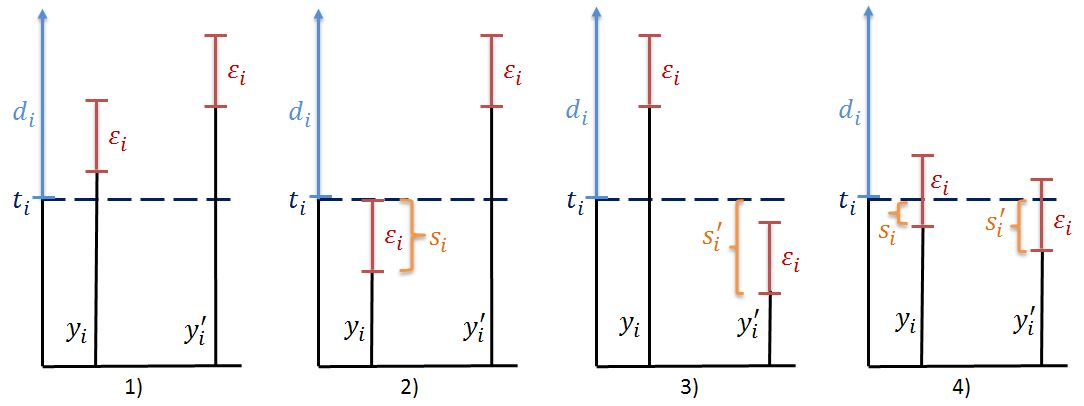
\includegraphics[width=1\textwidth]{Images/Chapter4/slack-variables}
\caption{ a) Graphic representation of slack variables for several scenarios where (1) $y_i, y'_i \geq t_i$, (2) $y_i \leq t_i < y'_i$, (3) $y'_i \leq t_i < y_i$ and (4) $y_i, y'_i < t_i$, adding $\epsilon_i$ to both $y_i$ and $y'_i$.}
\label{fig:2-2}
\end{figure}

\begin{defi}\label{chapMultiObjAlg:slacks}
Let us consider a goal $y_k \leq t_k$ over some measurable attribute $y_k$. The \textbf{slack variable} $s_k$ for this goal is defined as
\begin{equation}\label{eq:slack-def}
s_k = \max(0, t_k - y_k)
\end{equation}
Let us assume two vectors $\vec{y}, \vec{y'} \in \mathbb{R}^q$ and a level $j$ such that $d_j(\vec{y}) < d_j(\vec{y'})$. Let us denote 
$\Delta_j(\vec y, \vec{\epsilon}) = d_j(\vec{y} + \vec{\epsilon}) - d_j(\vec{y})$. Obviously, if \ $\vec{\epsilon} \succeq \vec{0}$, $\Delta_j(\vec y, \vec{\epsilon}) \geq 0$. We define the \textbf{cross-slack}  
$\delta_j(\vec{y},\vec{y'}) = \max_{\vec{\epsilon}\in \mathbb{R}^{+q}} (\Delta_j(\vec{y},\vec{\epsilon}) - \Delta_j(\vec{y'},\vec{\epsilon}))$, i.e. 
the greatest relative increment of the deviations of $\vec y$ and $\vec{y'}$ at level $j$ when adding any $\vec{\epsilon}\in \mathbb{R}^{+q}$. 
Notice that $\delta_j(\vec{y}, \vec{y'}) \geq 0$ and generally $\delta_j(\vec{y}, \vec{y'}) \neq \delta_j(\vec{y'}, \vec{y})$.

Each priority level $j$ comprises a set $I_j$ of one or more attributes $i$. Figure \ref{fig:2-2} shows that for each $i \in I_j$ four different cases can arise: (1) $y'_i, y_i \geq t_i$; (2) $y'_i \geq t_i$ and $y_i < t_i$; (3) $y'_i < t_i$ and $y_i \geq t_i$; (4) $y'_i, y_i < t_i$. It is straightforward that the greatest relative increment in cases 1 and 2 is 0, since the slack variable $s'_i$ equals $0$, while in cases 3 and 4, the greatest relative increment is 
$w_i \times (s'_i - s_i) = w_i \times (t_i - y'_i - (t_i - y_i)) =
w_i \times (y_i - y'_i)$. Therefore, an operative way of calculating the {\em cross-slack} $\delta_j(\vec{y}, \vec{y'})$ of $\vec{y}, \vec{y'}$ at level $j$ is

\begin{equation}\label{eq:slack-var}
    \delta_j(\vec{y}, \vec{y'}) = \sum_{k\in I_j} w_k \times \max(0, s'_k - s_k)
\end{equation}
\end{defi}

\begin{defi}\label{chapMultiObjAlg:pruningpreference}
We define the \textbf{pruning preference} $\prec_{P}$ by imposing on the lexicographical goal preference additional conditions concerning cross-slacks: 
    \begin{multline}\label{eq:cond-prune-new}
      \vec{y} \prec_{P} \vec{y'} \ \ \Leftrightarrow \ \ \exists j
      \ (d_j(\vec{y}) < d_j(\vec{y'}) \quad \land  \quad \delta_j(\vec{y}, \vec
      {y'}) < d_j(\vec{y'}) - d_j(\vec{y})    \\ \land      \quad \forall i < j
      \ \ (d_i(\vec{y}) = d_i(\vec{y'}) \ \quad \land \quad \delta_i(\vec{y}, \vec{y'}) = 0))
    \end{multline}
i.e., $\vec{y} \prec_{P} \vec{y'}$ when (i) $\vec{y} \prec_{G} \vec{y'}$;
(ii) the cross-slacks of  $\vec{y}$ and  $\vec{y'}$ are zero for the first levels (where deviations are the same); and (iii) for the first level where deviations differ, the cross-slack of $\vec{y}$ and $\vec{y'}$ is strictly smaller than the difference between deviations. 

It can be easily checked that $\prec_{P}$ is irreflexive and  transitive. Therefore $\prec_{P}$ is a partial order relation. We read $\vec{y} \prec_{P} \vec{y'}$ as <<$\vec y$ allows to prune $\vec{y'}$>>.
\end{defi}

Table \ref{tab:pseudocode-lexgo} introduces \lexgo, an exact label-setting multicriteria search algorithm for lexicographic goal preferences with lower bound estimates. The inputs are a multiobjective graph $G$, a start node $s$, a destination node $t$, a set of weighted goals grouped in pre-emptive priority levels, and a monotone distance estimate function. \lexgo \ outputs the solution subgraph with the set of all goal-optimal solution paths between $s$ and $t$. In a similar manner than most of the multicriteria search algorithms presented in Section \ref{chapMultiObjAlg:sec:MSP}, the following data structures are managed by the algorithm:

\begin{itemize}
   \item \textbf{SG}: A search graph that records partial solution paths emanating from $s$ and their costs. Each node $n$ in $SG$ stores the following information:
	\begin{itemize}
   		\item $G_{op}(n)$: Set of cost vectors (labels) $\vec{g}_n$ of paths reaching node $n$ which have not been explored yet.
 		\item $G_{cl}(n)$: Set of labels reaching node $n$ which have already been explored.
	\end{itemize}

	\item \textbf{OPEN}: A priority queue of unexplored labels. For each node $n$ in $SG$ and each cost vector $\vec{g_n} \in G_{op}(n)$, there is a label $(n, \vec{g_n})$ in OPEN. In fact, labels are extended to include also evaluation vectors and their deviation from goals. Each extended label $(n, \vec{d}_n, \vec{f}_n, \vec{g}_n)$ denotes that node $n$ is reached by a path with cost $\vec{g}_n$, deviation vector $\vec{d}_n$, and evaluation vector $\vec{f}_n$. We define $\vec{f}_n = \vec{g}_n + \vec{h}(n)$.
For the sake of simplicity, we will denote $\vec{d}(\vec{f}_n)$ as $\vec{d}_n$. Initially, $(s, \vec{d}_s, \vec{f}_s, \vec{g}_s)$ is the only label in OPEN. Labels in OPEN are sorted lexicographically according to deviation vectors. In case of ties they are ordered lexicographically according to evaluation vectors $\vec f$. This ensures that the first element in the queue has a goal-optimal evaluation among all $f_n$ in OPEN.
	
	\item \textbf{COSTS}: The set of cost vectors of solution paths found to the destination node.
	
    \item \textbf{Best achievement} vector $\bestd$ \ among all solutions already found.
\end{itemize} 

The structure of \lexgo \ is similar to previous label-setting multicriteria algorithms with label expansion, but incorporating elements of lexicographic goal preferences to guarantee that only a subset of the labels explored by a full multicriteria search will need to be explored.

\begin{table}
\caption{Pseudocode of \lexgo \ algorithm }
\scalebox{.95}{
\begin{tabular}{p{\columnwidth}}
\hline
\begin{enumerate}
\item CREATE:
  \par ---An empty search graph $SG$, and set $s$ as its root.
  \par ---Two sets $G_{cl}(s) = \emptyset$ and $G_{op}(s)=
  \{\vec{0}\}$.   
  \par ---A list of alternatives, OPEN = $\{(s, \vec{d}(\vec{h}(s)), \vec{h}(s), \vec{0}\}$.
  \par ---An empty set, COSTS.
  \par ---$\bestd = \vec{\infty}$, optimum achievement vector for solutions found.

\item \label{lexgo:label-selection} PATH SELECTION. If OPEN is not empty, then, 

  \par ---Select a label $(n, \vec{d}_n, \vec{f}_n, \vec{g}_n)$ from
  OPEN such that \newline $\nexists (n', \vec d_{n'}, \vec{f}_{n'},
  \vec{g}_{n'}) \in OPEN$ such that $\vec{f}_{n'} \prec_{G} \vec{f}_n$.

  \par ---Delete the selected label from OPEN, and move $\vec g_n$ from $G_{op}(n)$ to $G_{cl}(n)$. 
  
  \par ---If \ $\exists \vec{c^*} \in COSTS$ such that $\vec{c^*} \prec
  \vec{f}_n$,  then repeat step \ref{label-selection}  (lazy filtering)
  

\item CHECK TERMINATION. If OPEN is empty, or
  $\bestd \prec_{L} \vec{d}_n$, then backtrack in $SG$ from $t$
  and return the set of solution paths with costs in COSTS.

\item SOLUTION RECORDING. If $n$ is a destination node, then
    \par ---Include $\vec g_n$ in COSTS.
    \par ---$\bestd \longleftarrow \vec{d}_n$
    \par ---Go back to step \ref{lexgo:label-selection}.

\item \label{path-expansion}PATH EXPANSION: If $n$ is not a destination node, then for all successor nodes $m$ of $n$ do:
    \begin{enumerate}
    \item Calculate the cost of the new path found to $m$, its
      evaluation vector and deviation, $\vec{g}_m = \vec{g}_n +
      \vec{c}(n,m)$,  $\vec{f}_m = \vec{g}_m + \vec{h}(m)$,
      $\vec{d}_m = \vec{d}(\vec{f}_m)$.

    \item If no Pareto or deviation filtering (equations \ref{eq:cond-filter-dom} and \ref{eq:cond-filter-new}), then:
      \begin{itemize}
      \item If $m \notin SG$: 
	\begin{itemize}
	\item Add $(m, \vec{d}_m, \vec{f}_m, \vec{g}_m)$ to OPEN
	\item Set $G_{op}(m)= \{(\vec{g}_m)\}$.
	\item Label with $\vec{g}_m$ a pointer from $m$ to $n$.
	\end{itemize}
      \item else if $\vec{g}_m$ equals some cost vector in  $G_{op}(m) \cup G_{cl}(m)$ then
	\begin{itemize}
	\item Label with $\vec{g}_m$ a pointer from $m$ to $n$.
	\end{itemize}
      \item else if no Pareto or deviation pruning (equations \ref{eq:cond-prune-dom} and \ref{eq:cond-prune-deviation}), then:  
	\begin{enumerate}
   \item Eliminate vectors \ $\vec{g'}_{m} \in G_{op}(m)$ such that $\vec{g}_m \prec \vec{g'}_{m} \ \lor \ \vec{f}_m \prec_P \vec{g'}_{m} + \vec{h}(m)$, and their corresponding labels $(m, \vec{d'}_{m}, \vec{f'}_{m}, \vec{g'}_{m})$ from OPEN.
	\item Add $(m, \vec{d}_m, \vec{f}_m, \vec{g}_m)$ to OPEN,
          $\vec{g}_m$ to $G_{op}(m)$ and label with $\vec{g}_m$ a
          pointer from $m$ to $n$.
	\end{enumerate}
      \end{itemize}
	\item Go back to step \ref{lexgo:label-selection}.
    \end{enumerate}        
\end{enumerate}
\\
\end{tabular}
}
\label{tab:pseudocode-lexgo} 
\end{table}

The algorithm has five main steps. The first one is devoted to data structure initialization. The second one is devoted to label selection from OPEN. At each iteration, the algorithm selects the first label  $(n, \vec{d}_n, \vec{f}_n, \vec{g}_n)$ from OPEN, which has a goal-optimal evaluation vector $f_n$. The label is removed from OPEN, and moved from $G_{op}(n)$ to $G_{cl}(n)$. The third step recovers and returns the solution subgraph whenever some termination condition is satisfied. The fourth step records the solution whenever a destination node is selected. COSTS and $\bestd$ are updated accordingly. Finally, the selected label is expanded in step \ref{path-expansion}, i.e. all the extensions of the selected label are considered for inclusion in the search graph and the OPEN set. 

The algorithm iterates over steps 2, 3 , 4 and 5 until OPEN is empty, or $\vec{d}_B \prec_{L} \vec{d}_n$, i.e. all potential goal-optimal solutions have been examined. In such case, the algorithm terminates returning a solution subgraph, made up of all goal-optimal solution paths. COSTS stores the set of distinct goal-optimal costs.
 
During path expansion two different conditions may prevent an extension from consideration: filtering and pruning. These are described in detail below. 

%-------------------------------------------------------------------
\subsection{Pruning conditions}
\label{subsubsec:Pruning-conditions}
%-------------------------------------------------------------------

As already explained in Example \ref{ej:ejemplo-pruning1}, the optimality principle does not hold for lexicographic goal preferences. Therefore, pruning and filtering using goal preferences would not yield an admissible label setting algorithm in this case. 
Nevertheless, \lexgo \ includes two pruning conditions that improve search efficiency and, at the same time, guarantee that no goal-optimal solution will be pruned, (see Theorem \ref{chapFormalAnalysis:teo:lexgo-admissible} in Section \ref{chapFormalAnalysis:sec:admissibilityLexgo}):

\begin{itemize}

  \item 
Pareto pruning. As in other Pareto search algorithms like \namoa, we prune any dominated path to any node. A new label $(m, \vec d_m, \vec f_m, \vec g_m)$ to node $m$ is pruned whenever

    \begin{equation}\label{eq:cond-prune-dom}
      \exists \vec g \in G_{op}(m) \cup G_{cl}(m) \ | \ \vec g \prec \vec g_m 
    \end{equation}
    
  \item 
Deviation-based pruning. We propose an additional specific pruning condition based in the pruning preference defined by equation \ref{eq:cond-prune-new}. We prune a new label $(m, \vec d_m, \vec f_m, \vec g_m)$ to node $m$ whenever

\begin{equation}\label{eq:cond-prune-deviation}
\exists \vec g \in G_{op}(m) \cup G_{cl}(m) \ | \ \vec g + \vec h(m)\prec_P \vec f_m   
\end{equation}
\end{itemize}


\begin{ejemplo}\label{ej:ejemplo-pruning2}
Let us assume the same preference as in Example \ref{ej:ejemplo-pruning1} and two paths $P$ and $P'$ reaching the same node $n$ from $s$ with the following evaluation vectors:

\begin{center}
$\vec f = \vec{f}(P) = (22, 22, 12) \Rightarrow \ \vec{d}(P) = (2,1)$ \\
$\vec f' = \vec{f}(P') = (22, 18, 26) \Rightarrow \ \vec{d}(P') = (2,3)$
\end{center}

We observe that $\vec{d}(P) \prec_L \vec{d}(P')$. We can also easily check that the extra conditions for pruning, $\delta_1(\vec{f}, \vec{f}') = 0$ and $\delta_2(\vec{f}, \vec{f}') = 1 < 3 - 1 = 2$, also hold,


\begin{displaymath}
  \begin{array}{ll}
    \delta_1(\vec{f}, \vec{f}') & = 1 \times \max(0, s_1' - s_1) = \max(0, 0-0)  = 0 \\
    \delta_2(\vec{f}, \vec{f}') & = 0.5 \times \max(0, s_2' - s_2) + 0.5 \times \max(0, s_3' - s_3) \\
                               & = 0.5 \times \max(0, 2-0) + 0.5 \times \max(0, 0-8) \\
                               & = 1 \\
  \end{array}
\end{displaymath}

Therefore, path $P'$ will never lead to a better solution than $P$ and can be safely pruned.
\end{ejemplo}

%-------------------------------------------------------------------
\subsection{Filtering conditions}
\label{subsubsec:Filtering-conditions}
%-------------------------------------------------------------------

Filtering is the process of discarding labels that will never lead to a solution better than one already found. Two different conditions allow a label $(n, \vec{d}_n, \vec{f}_n, \vec{g}_n)$ to be filtered:

\begin{itemize}
   \item Pareto filtering. This is the standard dominance filtering in Pareto search algorithms:
     \begin{equation}\label{eq:cond-filter-dom}
     \exists \vec{c^*} \in COSTS \ | \ \vec{c^*} \prec \vec{f}_n
     \end{equation}

   \item Deviation based filtering. We introduce a specific filtering condition for goal-based preferences when a known solution has better goal satisfaction:
     \begin{equation}\label{eq:cond-filter-new}
     \bestd \prec_{L} \vec{d}_n
     \end{equation}
\end{itemize}

When a new solution is found, or the best achievement vector is updated, no new label satisfying the above conditions will be allowed to enter OPEN, however, those labels already in OPEN will not be straightforwardly discarded. This is due to \lexgo \ applies \emph{lazy filtering}. 
%In broad terms, lazy filtering consists of avoiding looking through OPEN to discard those labels which are dominated by the solution found, instead, filter those labels when they are selected for expansion, since the former is more time consuming than the latter (using a priority queue to store labels in OPEN as reference).

%-------------------------------------------------------------------
\subsection{Example}
\label{chapMultiObjAlg:subsubsec:example}
%-------------------------------------------------------------------

Let us now illustrate the algorithm with a simple example. Let us assume that the decision maker's preference involves two levels of goals: \\
 
Level 1 \hspace{10 mm} $cost_{1}(P) \leq 10, \hspace{5 mm} w_{1} = 0.5$ \\
\hphantom{a} \hspace{26 mm} $cost_{2}(P) \leq 10, \hspace{5 mm} w_{2} = 0.5$ 

Level 2 \hspace{10 mm} $cost_{3}(P) \leq 10, \hspace{5 mm} w_{3} = 1$ \\

Let us consider the sample graph in Figure \ref{fig:2-3}, where $s$ is the start node, and $t$ the destination node. A lower bound function $\vec{h}(n)$ has been calculated using the method proposed by Tung and Chew \citep{Tung1992} and is presented in Table \ref{tab:h-example1}. A trace of the OPEN list is shown in Table \ref{tab:trace-example1}. At each iteration the selected label is indicated with an arrow and pruned labels are crossed out.

\begin{figure}[!ht]
\centering
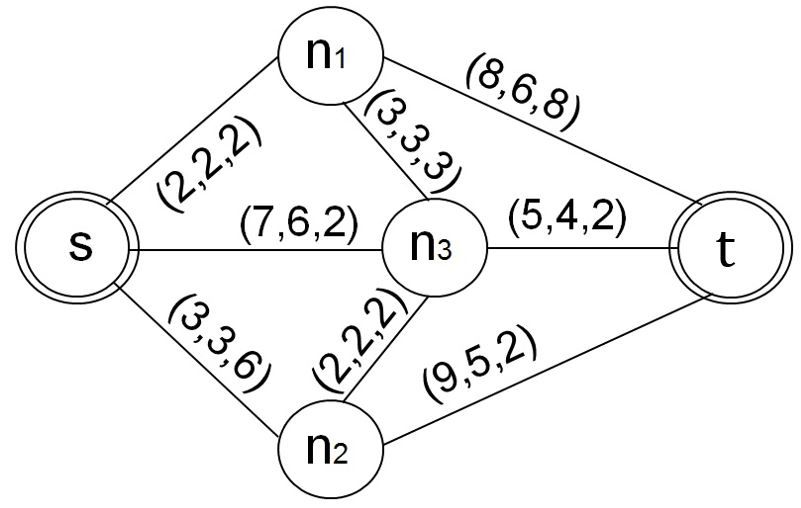
\includegraphics[width=0.5\textwidth]{Images/Chapter4/graph1}
\caption{Sample graph with satisfiable goals}
\label{fig:2-3}
\end{figure}

At iteration 1, SG has only node $s$ as its root and its corresponding label is selected from OPEN. Labels for the three descendants $n_1$, $n_2$ and $n_3$ of $s$ are added to OPEN. At iteration 2, two labels in OPEN have the same deviation vector, so the best lexicographic $\vec{f}$ is used to break the tie. Hence, the label to $n_1$ is selected. Its two successors $n_3$ and $t$ are added to OPEN. Addition of $n_3$ to $G_{op}(n_3)$ prunes the alternative already stored for $n_3$, since $(10,9,7) \prec_{P} (12,10,4)$. Notice that both evaluation vectors are non-dominated, however, the pruning condition presented in equation \ref{eq:cond-prune-deviation} is applied, since  $\delta_1((10,9,7),(12,10,4)) < d_1(12,10,4) - d_1(10,9,7) \ \Rightarrow \ 0 < 1-0$. At iteration 3, the label to $n_2$ is selected and expanded, generating new paths to the successors $n_3$ and $t$. The extension to $n_3$ is pruned, since the cost vector $(5,5,8)$ from path $(s, n_2, n_3)$ is dominated by the cost $(5,5,5)$ from path $(s, n_1, n_3)$. The second successor, $t$, is also pruned due to the existence of another label in $G_{op}(t)$ such that $(10,8,10) \prec_{P} (12,8,8)$. At iteration 4, the first path to a destination node is selected, the corresponding cost vector is added to COSTS $= \{ (10,8,10) \}$ and $\bestd$ is updated to $(0,0)$. This means that there is at least one path which satisfies all the goals provided. 

At iteration 5, $n_3$ is selected, and a new path to $t$ is generated and added to OPEN. At iteration 6, the only label in OPEN is selected. The cost vector $(10,9,7)$ represents another solution since $t$ is the destination node, its cost is not dominated by any vector in COSTS and it can also satisfy all goals. Finally, in the next iteration OPEN is empty and the algorithm would search backward from $t$ returning the solution subgraph with the two paths with costs (10,8,10) and (10,9,7).

\begin{table}
\caption{Lower bounds table with distance estimates of an example of \lexgo \ with satisfiable goals}
\centering
\begin{tabular}{cc}
\hline \noalign{\smallskip}
 n & $\vec h(n)$ \\
\noalign{\smallskip} \hline
$s$ & (10,8,4) \\
$n_1$ & (8,6,5)  \\
$n_2$ & (7,5,2)  \\
$n_3$ & (5,4,2)  \\
$t$ & (0,0,0)  \\
\hline
\end{tabular}
\label{tab:h-example1}
\end{table}

\begin{table}
\caption{Execution trace of an example of \lexgo \ with feasible goals (graph in Figure \ref{fig:2-3}).}
\centering
\begin{tabular}{ll}
\hline \noalign{\smallskip}
It & OPEN $(n,\vec{d},\vec{f},\vec{g})$ \\
\noalign{\smallskip} \hline
1 & $(s,(0,0),(10,8,4),(0,0,0))$ $\longleftarrow$ \\
\multirow{3}{*} {2} & $(n_1,(0,0),(10,8,7),(2,2,2))$ $\longleftarrow$\\
& $(n_2,(0,0),(10,8,8),(3,3,6))$ \\
& $(n_3,(1,0),(12,10,4),(7,6,2))$ \\
\multirow{4}{*} {3} & $(n_2,(0,0),(10,8,8),(3,3,6))$ $\longleftarrow$\\
& $(t,(0,0),(10,8,10),(10,8,10))$ \\
& $(n_3,(0,0),(10,9,7),(5,5,5))$ \\
& \sout{$(n_3,(1,0),(12,10,4),(7,6,2))$} \\
\multirow{4}{*} {4} & $(t,(0,0),(10,8,10),(10,8,10))$ $\longleftarrow$\\
& $(n_3,(0,0),(10,9,7),(5,5,5))$ \\
& \sout{$(n_3,(0,0),(10,9,10),(5,5,8))$} \\
& \sout{$(t,(1,0),(12,8,8),(12,8,8))$} \\
5 & $(n_3,(0,0),(10,9,7),(5,5,5))$ $\longleftarrow$\\
6 & $(t,(0,0),(10,9,7),(10,9,7))$ $\longleftarrow$ \\
7 & EMPTY SET\\
\hline
\end{tabular}
\label{tab:trace-example1}
\end{table}


%-------------------------------------------------------------------
\section{A dimensionality reduction technique for MSP}
\label{chapMultiObjAlg:sec:Time-efficient-MSalg}
%-------------------------------------------------------------------

This section describes a dimensionality reduction technique that speeds up the time performance of exact multicriteria search algorithms. Dimensionality reduction was first proposed as a space saving technique in the development of \emph{vector frontier search} \citep{Mandow2008,Mandow2009}, a blind multiobjective search algorithm that achieved impressive reductions in space requirements at the expense of increasing time requirements. This technique is used in this thesis showing that it can also be applied under reasonable assumptions to exact multicriteria search (and to \namoa \ and \lexgo \ in particular) to achieve important improvements in time performance. 

The key idea in dimensionality reduction is that, under a lexicographic order of expansion, dominance checks performed during filtering and certain pruning operations can be greatly simplified. We will start introducing the following useful terminology. We will say that  a vector $v$ is dominated by a set $X$ when there exists $v'\in X$ such that $v'\prec v$. Dominance checks performed on labels by \namoa (see Table \ref{ChapMultiObjAlg:tab:pseudocode-namoa}) can be stated as follows:
\begin{itemize}
    \item Filtering. Discard $(n,\vec g,\vec f)$ if $f$ is dominated by COSTS.
	 \item Op-pruning. Discard $(n,\vec g,\vec f)$ if $\vec g$ is dominated by $G_{op}(n)$.
	 \item Cl-pruning. Discard $(n,\vec g,\vec f)$ if $\vec g$ is dominated by $G_{cl}(n)$.
\end{itemize}

First we reproduce two definitions from \cite{Mandow2009}:

\begin{defi} \label{chapMultiObjAlg:def:tv}
Given a vector $ \vec v = (v_1, v_2, \ldots v_n)$, its \textbf{truncated vector} $ {t(\vec v)}$ is that vector $v$ without its first component, i.e. $ {t(\vec v)} = (v_2, \ldots v_n)$.
\end{defi}

\begin{defi} \label{chapMultiObjAlg:def:tv2}
Given a  set of vectors  $X$, its associated set of truncated vectors is  
$T(X) = \mathcal{N}(X)(\{ t(\vec x) | \; \vec x \in X\})$. 
\end{defi}

We call our reduction technique ``t-discarding'' (or \textit{truncated discarding}), since it is based on discarding cost vectors by their truncated cost vectors. 

\begin{defi}\label{chapMultiObjAlg:def:tv3}
Let $X$ be a set of vectors. A vector $\vec v$ is t-discarded by $X$ when for all $\vec{v'} \in X \ \ v'_1 \leq v_1$ and there is $\vec{v''}\in X$ such that $t(\vec{v''})\in T(X)$ and one of the following conditions holds:

a) $v''_1 < v_1$ and $t(\vec{v''}) \preceq t(\vec v)$; or

b) $v''_1 = v_1$ and $t(\vec{v''}) \prec t(\vec v)$.
\end{defi} 

\begin{ejemplo}
{\em
Figure \ref{fig:4-1} displays three cost vectors $ \vec x = (6, 2, 4)$, $ \vec y = (4, 4, 5)$, and $ \vec z = (2, 3, 6)$, and shows also their truncated vectors $ {t(\vec x)}$, $ {t(\vec y)}$, and $ {t(\vec z)}$. Notice that none of $\vec x, \vec y, \vec z$ dominates any of the others;
so $\mathcal{N}(X)=\{\vec x,\vec y,\vec z\}$. On the other hand the truncated vectors are $t(\vec x)=(2,4)$, $t(\vec y)=(4,5)$ and $t(\vec z)=(3,6)$. Since ${t(\vec y)}$ and ${t(\vec z)}$ are dominated by ${t(\vec x)}$ we have $T(X)= \{(2,4)\}$. 

Let us consider now  a vector $\vec w=(7,2,4)$. The standard dominance test would imply three vector comparisons in the worst case,
namely those of $\vec w$ against $\vec x, \vec y$ and $\vec z$. However, t-discarding implies just one vector comparison, that of $t(\vec w)$ against $t(\vec x)$.
Since $t(\vec x) \preceq t(\vec w)$ and $x_1 < w_1$, $w$ will be t-discarded by $X$.

Let us consider now vector $w'=(6,2,4)$. Let us check if $\vec{w'}$ is t-discarded by $X$. We have $t(\vec x) \preceq t(\vec{w'})$, but $x_1 \not< w'_1$, so condition (a) does not hold. Again, $t(\vec x) \not\prec t(\vec{w'})$, so condition (b) does not hold either, and in consequence $\vec{w'}$ is not t-discarded by $X$.
}
\end{ejemplo}

\begin{figure}%[ht]
\centering
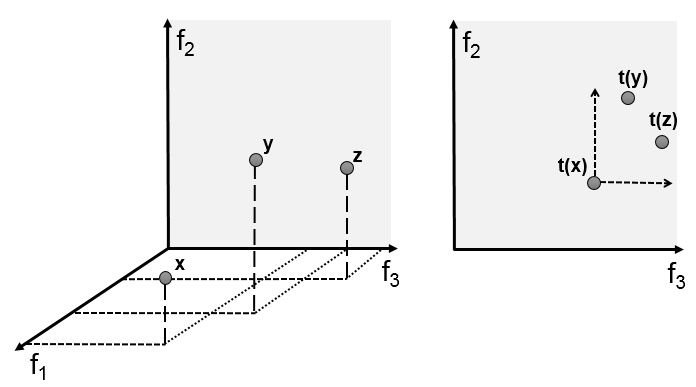
\includegraphics[width=0.75\textwidth]{Images/Chapter4/vectors}
\caption{A set of vectors $X = \{\vec x,\vec y,\vec z\}$ and its truncated vectors $t(\vec x),t(\vec y),t(\vec z)$.}
\label{fig:4-1}
\end{figure}

We propose a modification of filtering and/or cl-pruning checks and prove that the new version of the checks is equivalent to the original one, given some assumptions, see the formal proof in Section \ref{chapFormalAnalysis:sec:admissibilityNamoate}. An example concerning the impossibility of applying t-discarding to the op-pruning is shown in Section \ref{chapMultiObjAlg:subsec:namoate}, while the relative ratio of op-pruning, cl-pruning and filtering operations over the total number of discarded labels in our experiments over random grids and road maps can be seen in Figures \ref{fig:6-9} and \ref{fig:7-4}, respectively.

We present below the application of the t-discarding technique to \namoa. 
Moreover, let us emphasize that not only a priori multicriteria algorithms may benefit from this technique, we also review the application to \lexgo \ in Section \ref{chapMultiObjAlg:subsec:lexgote}.

%-------------------------------------------------------------------
\section{Algorithm \texorpdfstring{\namoate}{NAMOA*te}}
\label{chapMultiObjAlg:subsec:namoate}
%-------------------------------------------------------------------

Table \ref{ChapMultiObjAlg:tab:pseudocode-namoa-te} shows a slightly modified pseudocode of \namoa \ combined with the dimensionality reduction technique, i.e. \namoate. The newly added or modified pseudocode lines have been emphasized with a right arrow. Although \namoa \ uses a general lower bound function $H(n)$ that returns a set of vector estimates, \namoate \ employs a lower bound function $h(n)$, limited to a single vector estimate per node and that satisfies the monotone property (see Definition \ref{chapFormalAnalysis:def:multiObjmonotoneH}). \namoate \ uses the same data structures employed by \namoa, with the only addition of the sets T(COSTS) and $T(G_{cl}(n))$. 
%An example of \namoa \ run can be found in \citep[3.2]{Mandow2010} (the behaviour of \namoate \ is completely equivalent to \namoa).  

The new cl-pruning and filtering operations in \namoate \ employ the truncated set of vectors, instead of the original ones, to discard new labels. In addition, the truncated sets must be updated after each insertion of a new truncated vector. The equations corresponding to these operations are shown in Table \ref{ChapMultiObjAlg:tab:truncated-operations}. The update operation will be relatively costly depending on the size of the sets of truncated vectors. On the other hand, the size of the sets of truncated vectors over the size of the original ones defines the savings that can be achieved. This along with the frequency that op-pruning occurs shall define the efficiency of \namoate. We will analyze empirically the performance of \namoate \ in Sections \ref{chapEmpiricalAnalysis:sec:resultsgridsnamoate} and \ref{chapEmpiricalAnalysis:sec:resultsdimacsnamoate}. 

\begin{table}
\caption{New operations over truncated sets of vectors.}
\scalebox{.95}{
\begin{tabular}{p{\columnwidth}}
\hline
\begin{enumerate}
	\item Pareto pruning (dr). A label $(m,\vec f_m, \vec g_m)$ is pruned whenever     
		\begin{equation}\label{eq:trunc-cond-prune-dom-lexgo}
			\exists \vec v \in T(G_{cl}(m)) \ \ | \ \ v \prec t(\vec g_m) \qquad
			\lor \qquad \exists \vec g \in G_{op}(m) \ \ | \ \ \vec g \prec \vec g_m
		\end{equation}
	\item Pareto filtering (dr). A label $(m,\vec f_m, \vec g_m)$ is filtered whenever    
		\begin{equation}\label{eq:trunc-cond-filter-dom}
     		\exists \vec v \in T(COSTS) \quad | \quad \vec v \prec t(\vec f_m)
		\end{equation}
	\item Update set of truncated solution cost vectors. After inserting vector $\vec v$ in T(COSTS) do    
		\begin{equation}\label{eq:update-trunc-costs}
	      \text{Remove} \ \ \vec{v'} \in T(COSTS) \quad | \quad \vec v \prec \vec{v'}
		\end{equation}
	\item Update set of truncated permanent vectors. After inserting vector $\vec v$ in $T(G_{cl}(m))$ do
		\begin{equation}\label{eq:update-trunc-gcl}
	      \text{Remove} \ \ \vec{v'} \in T(G_{cl}(m)) \quad | \quad \vec v \prec \vec{v'}
		\end{equation}		
\end{enumerate}
\\
\end{tabular}
}
\label{ChapMultiObjAlg:tab:truncated-operations} 
\end{table}

Two important changes in the adaptation of \namoa \ should be noted. First, the lexicographic order is the mandatory label selection policy in \namoate \ to select between all non-dominated alternatives in OPEN, whilst \namoa \ can work out with any policy that assures the selected label is non-dominated. Moreover, \namoa \ has been previously reported to perform better under a linear aggregation policy than under a lexicographic one \citep{Machuca2011}. Second, in step \ref{ChapMultiObjAlg:pruning-namoa-te}, the original pseudocode of \namoa \ does not establish which pruning operation should be performed in the first place, over open or permanent labels, however, we plainly define the cl-pruning as the first operation to be made, to take advantage of the t-discarding technique before applying op-pruning. Concerning to op-pruning, let us now present an example to show why the new technique cannot be applied to the op-pruning operation.

\begin{table}
\caption{Pseudocode of $\text{NAMOA}_{dr}^*$ algorithm.}
\scalebox{.95}{
\begin{tabular}{p{\columnwidth}}
\hline
\begin{enumerate}
\item CREATE:
  \par --- An empty search graph SG, and place $s$ as its root.
  \par --- Two sets $G_{cl}(s) = \emptyset$ and $G_{op}(s)= \{(\vec{0})\}$.   
  \par --- A list of alternatives, OPEN = $\{(s, \vec{0}, \vec h(s)\} $.
  \par --- An empty set, COSTS.
  \par $\rightarrow$ Two empty sets of truncated vectors $T(G_{cl}(s))$ and T(COSTS).

\item \label{label-selection-namoa-te} PATH SELECTION. If OPEN is not empty, then, 

  \par $\rightarrow$ Select a label $(n, \vec g_n, \vec f_n) $ from OPEN such that $\nexists (n', \vec g_{n'}, \vec f_{n'}) \in$ OPEN such that $\vec f_{n'} \prec_L \vec f_n$.

  \par --- Delete the selected label from OPEN, and move $\vec g_n$ from $G_{op}(n)$ to $G_{cl}(n)$. 
  
  \par $\rightarrow$ Add $t(\vec g_n)$ to $T(G_{cl}(n))$ and update $T(G_{cl}(n))$ (equation \ref{eq:update-trunc-gcl}). 
  
  \par $\rightarrow$ If Pareto filtering (dr) $\vec f_n$ (equation \ref{eq:trunc-cond-filter-dom}), then repeat step \ref{label-selection-namoa-te}
  
\item CHECK TERMINATION. If OPEN is empty, then backtrack in SG from $\gamma$ and return the set of solution paths with costs in COSTS.

\item SOLUTION RECORDING. If $n$ is a destination node, then
    \par Include $\vec g_n$ in COSTS and 
    \par $\rightarrow$ Add $t(\vec g_n)$ to T(COSTS) and update T(COSTS) (equation \ref{eq:update-trunc-costs}). 
    \par --- Go back to step \ref{label-selection-namoa-te}.

\item PATH EXPANSION: If $n$ is not a destination node, then for all successor nodes $m$ of $n$ do:
  \begin{enumerate}
    \item Calculate the cost of the new path found to $m$ and its lower bound, \newline 
    $\vec g_m = \vec g_n + \vec c(n,m)$ and $\vec f_m = \vec g(m) + \vec h(m)$.
    \item $\rightarrow$ Unless Pareto filtering (dr) $\vec f_m$ (equation \ref{eq:trunc-cond-filter-dom}):
      \begin{enumerate}
      \item If $m \notin$ SG: 
	\begin{itemize}
	\item Set $G_{op}(m)= \{(\vec g_m)\}$ and add $(m, \vec g_m, \vec f_m)$ to OPEN.
	\item Label with $\vec g_m$ a pointer from $n$ to $m$.
	\end{itemize}
      \item else if $\vec g_m$ equals some cost vector in  $G_{op}(m) \cup G_{cl}(m)$ then
	\begin{itemize}
	\item Label with $\vec g_m$ a pointer from $n$ to $m$.
	\end{itemize}
      \item \label{ChapMultiObjAlg:pruning-namoa-te} $\rightarrow$ else unless Pareto pruning (dr) (eq \ref{eq:update-trunc-costs}):  
	\begin{itemize}
   \item Eliminate vectors $\vec g_{m'} \in G_{op}(m)$ such that $g_m \prec \vec g_{m'}$ and its corresponding label $(m, \vec g_{m'}, \vec f_{m'})$ from OPEN.
	\item Add $(m, \vec g_m, \vec f_m)$ to OPEN, $\vec g_m$ to $G_{op}(m)$ and label with $\vec g_m$ a pointer from $n$ to $m$.
	\end{itemize}
      \end{enumerate}
    \item Go back to step \ref{label-selection-namoa-te}.
  \end{enumerate}
\end{enumerate}
\\
\end{tabular}
}
\label{ChapMultiObjAlg:tab:pseudocode-namoa-te} 
\end{table}

\begin{ejemplo}\label{chapMultiObjAlg:ej:op-pruning}
Figure \ref{fig:2-4} displays a sample graph with three objectives. Let us assume for the sake of clarity that $\vec h(n) = \vec 0$. At iteration 1, $s$ is expanded and its two extended paths $s \rightarrow n_1$ and $s \rightarrow n_2$ stored in OPEN. At iteration 2, label $(n_1, (1,1,1), (1,1,1))$ is expanded and label $(n_3, (4,4,4), (4,4,4))$ recorded in $G_{op}(n_3)$. In case t-discarding were applied to op-pruning, $T(G_{op}(n_3)) = \{ (4,4) \}$. At the next iteration label $(n_2,$ $(2,2,2), (2,2,2))$ is expanded according to the lexicographic selection order. 

The new generated path, $s \rightarrow n_2 \rightarrow n_3$, with label $(n_3, (3,5,5), (3,5,5))$ is non-dominated with respect to $(n_3, (4,4,4), (4,4,4))$, however, if we apply op-pruning the truncated vector $(5,5)$ corresponding to label $(n_3, (3,5,5), (3,5,5))$ would be t-discarded by truncated vector $(4,4)$ corresponding to label $(n_3, (4,4,4), (4,4,4))$. Logically, the first component of the new generated label does not necessarily have its first component equal or greater than all the open labels reaching the node (on the contrary, a lexicographic order and a consistent lower bound function can guarantee that for the permanent labels), therefore, t-discarding cannot be applied to op-pruning.
\end{ejemplo}

\begin{figure}%[ht]
\centering
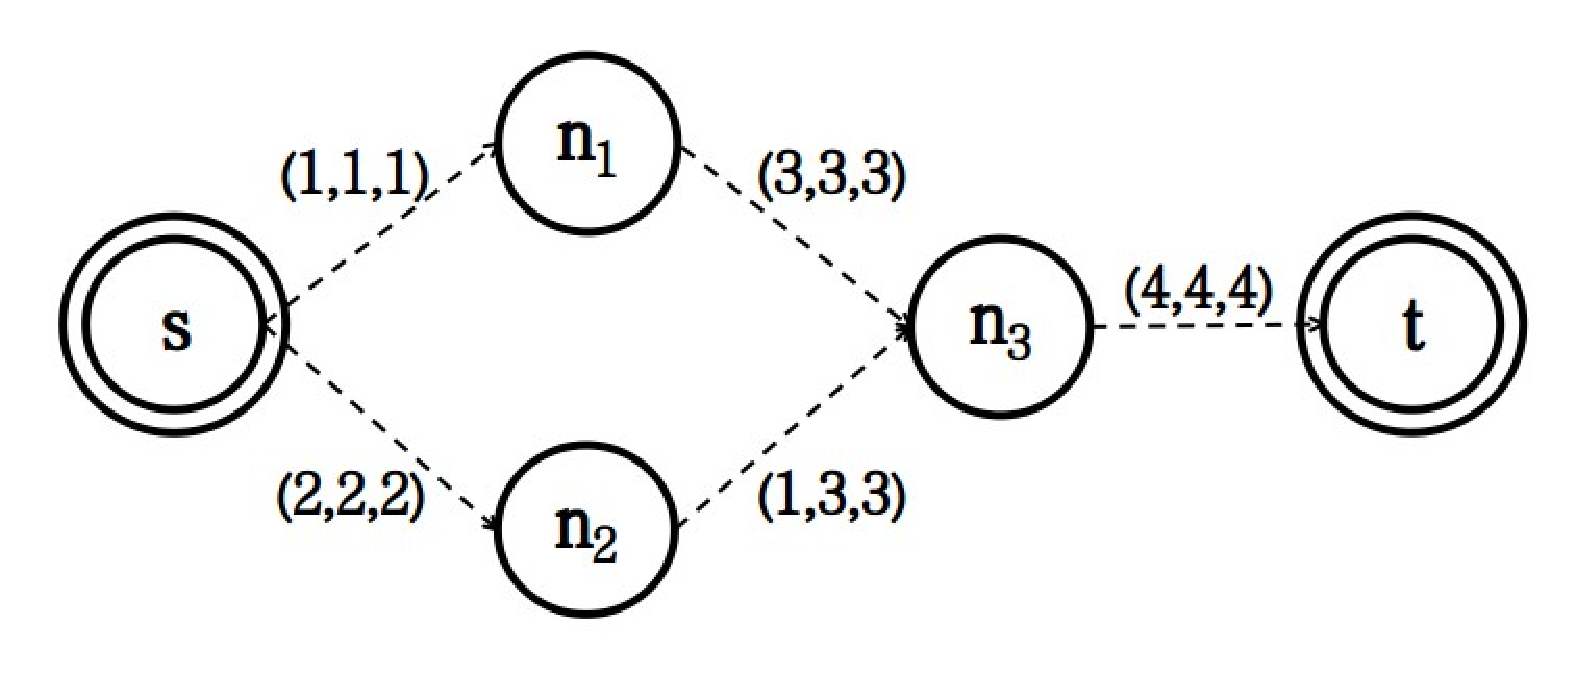
\includegraphics[width=0.65\textwidth]{Images/Chapter4/example-op-pruning}
\caption{Sample graph one with 3 objectives.}
\label{fig:2-4}
\end{figure}

%-------------------------------------------------------------------
\section{Algorithm \texorpdfstring{\lexgote}{LEXGO*te}}
\label{chapMultiObjAlg:subsec:lexgote}
%-------------------------------------------------------------------

Table \ref{tab:pseudocode-lexgo-te} displays the pseudocode of \lexgo \ adapted to incorporate the t-discarding procedure, i.e. the version that employs the dimensionality reduction technique, called \lexgote. A right arrow emphasizes the added or modified lines. The algorithm also uses the same monotone lower bound function $\vec h(n)$ and data structures employed by \lexgo, with the addition of T(COSTS) and $T(G_{cl}(n))$. An example of use of \lexgo \ was presented in Section \ref{chapMultiObjAlg:subsubsec:example} (the behavior of \lexgote \ does not differ from the behavior of \lexgo). 

\lexgo, like \namoa, can use any label selection policy as long as the selected labels are always guaranteed to be non-dominated. Nevertheless, \lexgote \ must employ the lexicographic order. This restricts the scenarios where cl-pruning and filtering operations can be applied to those where all permanent paths reaching a node have zero deviation for all priority levels, i.e. we define the scenario where t-discarding technique can be applied to \lexgote \ as follows:
\begin{equation}\label{eq:trunc-cond-prune-dom-lexgote}
	\forall n \ \ \forall l_n = (n, \vec d_n, \vec f_n, \vec g_n) \in (G_{cl}(n)) \quad \vec d_n = \vec 0 \quad \land \quad \forall \vec{c^*} \in COSTS \quad \vec{d}(\vec{c^*}) = \vec 0
\end{equation}
In this case, the set of labels expanded by \lexgo \ and \lexgote \ will be equivalent and they will be expanded exactly in the same order. Therefore, we will apply t-discarding to filtering or cl-pruning whenever all the labels in the set satisfy the condition to have a null deviation from goals. Since labels are expanded in lexicographic order, as soon as the first label with a positive  deviation is selected, \lexgote \ will change its filtering and cl-pruning to the regular one. We present an example of this phenomenon below. The analyses concerning the time performance of \lexgote \ over the other presented algorithms will be further studied empirically and formally in Section \ref{chapFormalAnalysis:sec:analysisLexgote}. 

\begin{table}
\caption{Pseudocode of \lexgote \ algorithm.}
\scalebox{.92}{  
\begin{tabular}{p{\columnwidth}}
\hline
\begin{enumerate}
\item CREATE:
  \par ---An empty search graph $SG$, and set $s$ as its root.
  \par ---Two empty sets $G_{cl}(s)$ and COSTS, and $G_{op}(s)=
  \{\vec{0}\}$.   
  \par ---A list of alternatives, OPEN = $\{(s, \vec{d}(\vec{h}(s)), \vec{h}(s), \vec{0}\}$.
  \par $\rightarrow$ Two empty sets of truncated vectors $T(G_{cl}(s))$ and T(COSTS).
  \par ---$\bestd = \vec{\infty}$, optimum achievement vector for solutions found.
  \par $\rightarrow$ A variable \textit{sat = TRUE} to record whether goals are satisfied or not. 

\item \label{lexgo-te:label-selection} PATH SELECTION. If OPEN is not empty, then, 

  \par Select a label $(n, \vec{d}_n, \vec{f}_n, \vec{g}_n)$ from
  OPEN s.t. \newline 
  $\nexists (n', \vec d_{n'}, \vec{f}_{n'}, \vec{g}_{n'}) \in OPEN$ \ | \ $\vec{f}_{n'} \prec_{G} \vec{f}_n$.

  \par ---Delete the selected label from OPEN, and move $\vec g_n$ from $G_{op}(n)$ to $G_{cl}(n)$. 
  
  \par $\rightarrow$ If $\vec d \neq \vec 0$ then \textit{sat = FALSE}.
  
  \par If \textit{sat == TRUE} then $t(\vec g_n)$ to $T(G_{cl}(n))$ and update $T(G_{cl}(n))$ (equation \ref{eq:update-trunc-gcl}). 
  	\begin{itemize}
  		\item If Pareto filtering (dr) $f_n$ (equation \ref{eq:trunc-cond-filter-dom}), then repeat step \ref{lexgo-te:label-selection}
  	\end{itemize}

  \par $\rightarrow$ Else if Pareto filtering (equation \ref{eq:cond-filter-dom}) then repeat step \ref{lexgo-te:label-selection}  
	  
\item CHECK TERMINATION. If OPEN is empty, or
  $\bestd \prec_{L} \vec{d}_n$, then backtrack in $SG$ from $t$
  and return the set of solution paths with costs in COSTS.

\item SOLUTION RECORDING. If $n$ is a destination node, then
    \par $\rightarrow$  Include $\vec g_n$ in COSTS and $\bestd \longleftarrow \vec{d}_n$
    \par $\rightarrow$ If \textit{sat} is TRUE add $t(\vec g_n)$ to T(COSTS) and update it (equation \ref{eq:update-trunc-costs}). 
    \par ---Go back to step \ref{lexgo-te:label-selection}.

\item PATH EXPANSION: If $n$ is not a destination node, then for all successor nodes $m$ of $n$ do:
    \begin{enumerate}
    \item Calculate the cost of the new path found to $m$, its evaluation vector and deviation, $\vec{g}_m = \vec{g}_n + \vec{c}(n,m)$,  $\vec{f}_m = \vec{g}_m + \vec{h}(m)$, $\vec{d}_m = \vec{d}(\vec{f}_m)$.
    \item If no Pareto or deviation filtering (equations \ref{eq:cond-filter-dom} (or \ref{eq:trunc-cond-filter-dom} when \textit{sat == TRUE}) and \ref{eq:cond-filter-new}), then:
      \begin{itemize}
      \item If $m \notin SG$: 
	\begin{itemize}
	\item Add $(m, \vec{d}_m, \vec{f}_m, \vec{g}_m)$ to OPEN
	\item Set $G_{op}(m)= \{(\vec{g}_m)\}$.
	\item Label with $\vec{g}_m$ a pointer from $m$ to $n$.
	\end{itemize}
      \item else if $\vec{g}_m$ equals some cost vector in  $G_{op}(m) \cup G_{cl}(m)$ then
	\begin{itemize}
	\item Label with $\vec{g}_m$ a pointer from $m$ to $n$.
	\end{itemize}
      \item else if no Pareto or deviation pruning (equations \ref{eq:cond-prune-dom} (or \ref{eq:trunc-cond-filter-dom} when \textit{sat == TRUE}) and \ref{eq:cond-prune-deviation}), then:  
	\begin{enumerate}
   \item Eliminate vectors \ $\vec{g'}_{m} \in G_{op}(m) \ \ |
          \ \ \vec{g}_m \prec \vec{g'}_{m} \ \lor \ \vec{f}_m \prec_P \vec{g'}_{m} + \vec{h}(m)$, and their corresponding labels $(m, \vec{d'}_{m}, \vec{f'}_{m}, \vec{g'}_{m})$ from OPEN.
	\item Add $(m, \vec{d}_m, \vec{f}_m, \vec{g}_m)$ to OPEN,
          $\vec{g}_m$ to $G_{op}(m)$ and label with $\vec{g}_m$ a
          pointer from $m$ to $n$.
	\end{enumerate}
      \end{itemize}
	\item Go back to step \ref{lexgo-te:label-selection}.
    \end{enumerate}        
\end{enumerate}
\\
\end{tabular}
}
\label{tab:pseudocode-lexgo-te} 
\end{table}

\begin{figure}%[ht]
\centering
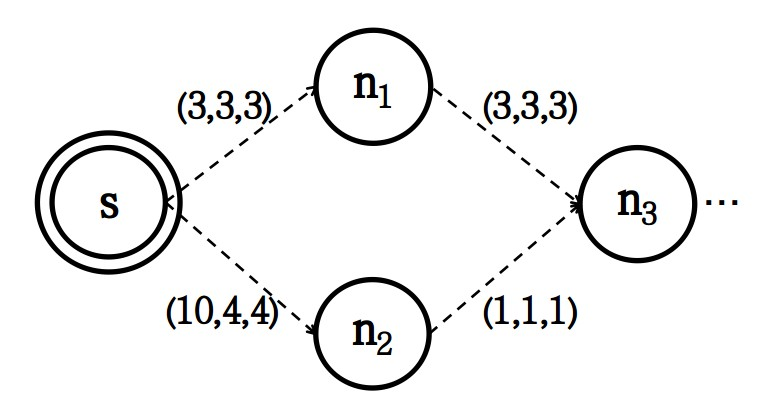
\includegraphics[width=0.5\textwidth]{Images/Chapter4/example-dev-op-pruning}
\caption{Sample graph two with 3 objectives.}
\label{fig:2-5}
\end{figure}

\begin{ejemplo}\label{chapMultiObjAlg:ej:dev-op-pruning}
Figure \ref{fig:2-5} displays a sample partial graph with three objectives. Let us assume that $\vec h(n) = \vec 0$ and the lexicographic goals are the ones presented in Section \ref{chapMultiObjAlg:subsubsec:example}. At iteration 1, $s$ is expanded and its two extended paths $s \rightarrow n_1$ and $s \rightarrow n_2$ stored in OPEN and labels ($n_1$, (0,0), (3,3,3), (3,3,3)) and ($n_2$, (0,0), (10,4,4), (10,4,4)), stored in $G_{op}(n_1)$ and $G_{op}(n_2)$, respectively.

At iteration 2, label ($n_1$, (0,0), (3,3,3), (3,3,3)) is expanded and label ($n_2$, (0,0), (6,6,6), (6,6,6)) recorded in $G_{op}(n_3)$. Thus,  At iteration 3, label ($n_3$, (0,0), (6,6,6), (6,6,6)) is expanded, since the concatenation of its deviation and evaluation vectors ($\vec d \cdot \vec f$) is lexicographically better than the other alternative in OPEN, ($n_2$, (0,0), (10,4,4), (10,4,4)), and added to $G_{cl}(n_3)$.

At iteration 4, label ($n_2$, (0,0), (10,4,4), (10,4,4)) is expanded and its extension ($n_2$, (0.5,0), (11,5,5), (11,5,5)) is checked for a cl-pruning operation against $G_{cl}(n_3) = \{((0,0), (6,6,6), (6,6,6)) \}$. If we do not pay attention to the fact that not all deviation vectors of labels in $n_3$ are zero, the condition to t-discard this path applies, i.e. $(5,5) \prec (6,6)$, but it is obvious that $(11,5,5) \nprec (6,6,6)$. 
\end{ejemplo}



%---------------------------------------------------------------------
%
% Chapter 5: Formal Analysis of Multicriteria Algorithms
%
%---------------------------------------------------------------------
%
% ChapFormalAnalysis.tex
% Copyright 2015 Dr. Francisco J. Pulido
%
% This file belongs to the PhD titled "New Techniques and Algorithms for Multiobjective and Lexicographic Goal-Based Shortest Path Problems", distributed under the Creative Commons Licence Attribution-NonCommercial-NoDerivs 3.0, available in http://creativecommons.org/licenses/by-nc-nd/3.0/. The complete PhD dissertation is freely accessible from http://www.lcc.uma.es/~francis/
%
% This thesis has been written adapting the TeXiS template, a LaTeX template for writting thesis and other documents. The complete TeXiS package can be obtained from http://gaia.fdi.ucm.es/projects/texis/. TeXis is distributed under the same conditions of the LaTeX Project Public License (http://www.latex-project.org/lppl.txt). The complete license is available in http://creativecommons.org/licenses/by-sa/3.0/legalcode
%
%---------------------------------------------------------------------

\chapter{Formal Analysis of Multicriteria Algorithms}
\label{chapFormalAnalysis}

\begin{FraseCelebre}
\begin{Frase}
Make everything as simple as possible, but not simpler.
\end{Frase}
\begin{Fuente}
Albert Einstein (1879-1955)
\end{Fuente}
\end{FraseCelebre}
%
%\begin{resumen}
%

In this chapter we aim to give a formal analysis of the multiobjective algorithms introduced in Chapter \ref{chapContributions}. We look for the best algorithmic alternative when goal-based preferences are given by an user to characterize the optimal solution subset. Two possibilities arise here. The first, obvious one, is to calculate the whole Pareto set using a multiobjective search algorithm like \namoa \ and extract a posteriori the subset of Pareto solutions which satisfy the goals. A second alternative is to concentrate the search effort only in the goal-optimal solutions, i.e. discard from the first stages of the search those paths which will not lead to satisfy the goals or minimize the deviation from them. This thesis has introduced one such algorithm, called \lexgo. 
%a multicriteria search algorithm developed to concentrate search effort on goal-optimal solutions.

Both algorithms, \namoa \ and \lexgo \ may share the same label selection procedure and filtering/pruning processes, though \lexgo \ introduces extra processes of pruning and filtering considering the deviation from goals, which will be formally studied further in this section. 

Another algorithmic contribution introduced in Chapter \ref{chapContributions} is the introduction of a new method, t-discarding, to speed up dominance checks. This method can be applied to the pruning and filtering checks keeping the admissibility of the algorithm. This technique has been applied to multiobjective and goal-based search, yielding two new algorithms: 
\namoate \ and \lexgote. Their properties are also analyzed in this section. 

We organize the relevant formal properties for a multicriteria search algorithm as follows: 

\begin{description}
    \item[Admissibility] 

All algorithms introduced in this thesis are theoretically proven to be admissible. The formal proofs on the admissibility of \namoa \ were presented in \citep{Mandow2005, Mandow2010}. \lexgo \ properties of admissibility will be presented further in Section \ref{chapFormalAnalysis:sec:analysisLEXGO}. Finally, the t-discarding technique which is employed in \namoate \ and \lexgote \ is analyzed in Section \ref{chapFormalAnalysis:sec:analysisNAMOATE}. 

    \item[Efficiency] 

A standard in formal analyses to measure the efficiency of multicriteria search algorithms is the number of explored labels. A recent study showed that \namoa \ is optimal according to this measure when used with consistent lower bounds \citep{Mandow2010}. \namoa \ has been shown to expand an equal or smaller number of labels when using more informed consistent lower bound functions \citep{Mandow2010}. \lexgo, in particular, always expands a subset of the labels expanded by \namoa, see Section \ref{chapFormalAnalysis:sec:efficiencyLexgo} for further details. 

The number of explored labels can be a good measure of the space requirements of the algorithms. However, in multicriteria search the time requirements are influenced by other factors as well. The algorithms that use t-discarding expand the same set of labels as the traditional ones. However, the experimental evaluation reveals that the time performance is greatly improved. Therefore, we also analyze another important measures for the time performance of multicriteria search, the number of dominance comparisons and the cardinality of the non-dominated sets used to check dominance. These are the key of the impressive performance of the t-discarding technique. 

\end{description}

This chapter is organized as follows. Section \ref{chapFormalAnalysis:sec:analysisNAMOA} summarizes formal properties of \namoa. The same aspects are comparatively analyzed for \lexgo \ in Section \ref{chapFormalAnalysis:sec:analysisLEXGO}. Finally, the t-discarding technique is formally proved to be time efficient and characterized employing \namoate \ and \lexgote \ as examples of use. Finally, a brief discussion is presented. 

%-------------------------------------------------------------------
\section{Formal characterization of \texorpdfstring{\namoa}{NAMOA*}}
\label{chapFormalAnalysis:sec:analysisNAMOA}
%-------------------------------------------------------------------

The formal properties of \namoa \ have been recently introduced by \citet{Mandow2010} and further studied by \citet{Machuca2012a}. In this section, 
we briefly review previous theoretical properties of \namoa, since it is the basis on which \lexgo \ has been devised. This will allow us to analyze only the new features brought by \lexgo, the t-discarding technique and their implications on the admissibility and efficiency.

%-------------------------------------------------------------------
\subsection{Admissibility}
\label{chapFormalAnalysis:sec:admissibilityNamoa}
%-------------------------------------------------------------------

The results that follows are taken from  \citet{Mandow2010} and \citet{Machuca2012a}.

\begin{property}[Admissibility]\label{chapFormalAnalysis:prop:multiObjAdmissibilityNamoa}

When the graph $G=(N,A)$ is locally finite and $H(n)$ is a lower bound (admissible) the search is considered \textbf{admissible}, i.e. it is guaranteed to find \textbf{all non-dominated} optimal solutions, or does not terminate if there are infinite solutions. \namoa \ is admissible even on infinite graphs with some additional assumptions:

\begin{description}\label{chapFormalAnalysis:eq:multiObjAdmissibilityCondNamoa}
  \centering      
\item[a)] 
$\forall n \in N \land \forall \vec h =(h_1,\ldots ,h_q) \in H(n), \quad \forall k \in [1,q], \ h_k(n) \geq 0$
	 \item[b)] 
$\forall (n,n') \in A,  \land \forall \vec  c(n,n') \in \vec c, \quad \forall k \in [1,q], \ c_k(n,n') \ \geq \epsilon > 0$  
\end{description}
\end{property}

Several important properties of \namoa \ follow. These are analogous to those of the single objective A$^*$ algorithm.

\begin{teorema} \label{chapFormalAnalysis:teo:multiObjAdmissibility-teorema1Namoa} \citep[Theorem 4.2]{Mandow2010}
 For each non-dominated solution path
  $P^*=(s, n_1,\ldots, n_i, n_{i+1}\ldots \gamma)$ with cost $\vec
  g(P^*) = \vec c^{~*}$, there is always before its discovery a subpath
  $P_{i}^*=(s, n_1, \ldots,n_i)$  of $P^*$ such that: 
\begin{description}
  \centering  
    \item[a)]$P_{i}^*$ is recorded in $SG$
    \item[b)]$\ \vec g(P_{i}^*) \in G_{op}(n_i)$ \ \ \ \ \ \ \
    \item[c)]$\exists  \vec f \in F(P_{i}^*) \ | \ \vec f \preceq \vec c^{~*}$
\end{description}
That is to say the algorithm never discards Pareto optimal solutions.

\end{teorema}

\begin{teorema} \label{chapFormalAnalysis:teo:multiObjAdmissibility-teorema2Namoa} 
\citep[Theorem 4.3]{Mandow2010}
If there is at least a solution path $P^*$, the algorithm terminates even on infinite graphs.
\end{teorema}

\begin{corolario} \label{chapFormalAnalysis:corol:multiObjAdmissibility-corolario1Namoa} 
\citep[Corollary 4.4]{Mandow2010}
Whenever there is at least a solution path $P^*$, the set of non-dominated solution costs $C^*$ is finite.
\end{corolario}

\begin{lema}\label{chapFormalAnalysis:lem:multiObjAdmissibility-lema1Namoa} 
\citep[Lemma 4.5]{Mandow2010}
Each path $P \in \mathbb{P}_{sn}$  selected from $OPEN$ for expansion
  satisfies upon selection that,
\begin{equation}
%$
\exists \vec h \in H(n) \quad | \quad \nexists \vec c^{~*} \in C^*,
  \quad \vec c^{~*}\prec
  \vec g(P) + \vec h
%$
\end{equation}
\end{lema}

\begin{teorema}\label{chapFormalAnalysis:teo:multiObjAdmissibility-teorema4Namoa} 
\citep[Theorem 4.6]{Mandow2010}
A dominated solution can never be selected for expansion.
\end{teorema}

\begin{corolario} \label{chapFormalAnalysis:corol:multiObjAdmissibility-corolario2Namoa} 
\citep[Corollary 4.7]{Mandow2010}
The set of found solution vectors, COSTS, is at any time a subset of the set of all non-dominated solution cost vectors, i.e. $COSTS \subseteq C^*$.
\end{corolario}

\begin{teorema}\label{chapFormalAnalysis:teo:multiObjAdmissibility-teorema5Namoa} 
\citep[Theorem 4.9]{Mandow2010}
Since \namoa \ satisfies all the above conditions, \namoa \ is admissible.
\end{teorema}

Admissibility (i.e. the algorithm is exact and returns the whole set of solutions to the problem) is an important property. However, it is also important to prove that the efficiency of the algorithm improves with more precise lower bounds. 

%-------------------------------------------------------------------
\subsection{Efficiency of lower bounds and optimality}
\label{chapFormalAnalysis:sec:efficiencyNamoa}
%-------------------------------------------------------------------

Pathological behavior has been observed in another multiobjective search algorithm called \moa \ \citep{stewartwhite1991}. Although \moa \ is admissible, it has been proven to decrease performance in certain cases with more informed lower bounds \citep{PerezdelaCruz2013}. Fortunately, \namoa \ has been proven to enjoy efficiency properties analogous to those of \astar.

\begin{defi}\label{chapFormalAnalysis:def:multiObjc-acotado}
\citep[Definition 5.1]{Mandow2010}
A path $P= (s = n_0, n_1, n_2,\ldots, n_k)$ is said to be
\textbf{C-bounded} with respect to $H(n)$ (or C(H)-bounded) if for all subpaths $P_i =(n_0, n_1,\ldots,n_i)$ of $P$ it holds that:
\begin{equation}
\exists \vec h \in H(n_i) \quad | \quad \nexists \vec c \in C, \quad
\vec c \prec \vec g(P_i) + \vec h   
\end{equation}
\end{defi}

By definition, a $C^*$-bounded path will never be filtered (see Lemma \ref{chapFormalAnalysis:lem:multiObjAdmissibility-lema1Namoa} and Theorem \ref{chapFormalAnalysis:teo:multiObjAdmissibility-teorema4Namoa}). Therefore, such paths will be either selected for expansion or pruned.

\begin{teorema}\label{chapFormalAnalysis:teo:multiObjAdmissibility-teorema6Namoa}
\citep[Theorem 5.9]{Mandow2010} 
If $H(n)$ is consistent, then a \textbf{necessary and sufficient} condition
for \namoa \ to select some path $P =(s,\ldots,n)$ for expansion is
that: 
\begin{description}
  \centering  
    \item[a)]$P$ be a non-dominated path from $s$ to $n$
    \item[b)]$P$ be $C^*$-bounded \quad \quad  \quad \quad \quad \quad \quad \quad \quad \quad \
\end{description}
\end{teorema}

\begin{teorema}\label{chapFormalAnalysis:teo:multiObjAdmissibility-teorema7Namoa}
\citep[Theorem 5.10]{Mandow2010} 
 Let $H_1(n)$ and $H_2(n)$ be two admissible lower bounds for the same
  problem. Let $H_2(n)$ be additionally \textbf{monotone}. Let
  $NAMOA^*_1$ and $NAMOA^*_2$ be two versions of \namoa \ that differ
  only in the use of different lower bound functions $H_1(n)$ and $H_2(n)$
  respectively. If $H_2(n)$ is at least as informed as $H_1(n)$, then
  \textbf{all} paths selected for expansion by $NAMOA^*_2$ will also be
  selected for expansion by $NAMOA^*_1$.
\end{teorema}

\begin{property}[Efficiency]\label{chapFormalAnalysis:prop:multiObjEfficiency}

When $\forall n \in N, \  H(n) = \{ \vec 0 \}$, \namoa \ is analogous to the blind algorithm of \citet{Martins1984} or \citet{Raith2009}. When $H(n)$ is \textbf{consistent} or \textbf{monotone}, only the strictly necessary $C^*$-bounded paths will be expanded, and the pruning of those $C^*$-bounded paths not belonging to non-dominated solutions will be maximal, analogously to the single-objective case. If the costs of some optimal solution is denoted by vectors $\vec c^{~*}$, \namoa \ will always expand for sure all labels with some $\vec f(n) \prec \vec  c^{~*}$. Given consistent lower bound functions,  more actual suboptimal alternatives can be pushed out of the Pareto frontier with \textbf{more informed} lower bounds, reducing search effort.
\end{property}

\begin{property}[Optimality]\label{chapFormalAnalysis:prop:multiObjOptimality}
\namoa \ has been proved to be optimal in the number of path expansions among the class of exact best-first algorithms when using consistent distance estimates \citep{Mandow2010}, i.e. no algorithm in this class provided only with the same information could avoid exploring a single label explored by \namoa \ without compromising admissibility.
\end{property}

%-------------------------------------------------------------------
\section{Formal characterization of \texorpdfstring{\lexgo}{LEXGO*}}
\label{chapFormalAnalysis:sec:analysisLEXGO}
%-------------------------------------------------------------------

This section proves some relevant properties of \lexgo. First, we will show that \lexgo \ is at least as \emph{efficient} as \namoa \ in terms of label expansions, i.e. it always expands a subset of the labels expanded by \namoa. Then, we will show that it is \emph{admissible}, i.e. it always returns the set of all goal-optimal solutions. Again, these properties are analogous to those of the single objective \astar \ search algorithm. 

The proofs presented in this section rely on a set of reasonable
assumptions, analogous to those presented in Section  \ref{chapFormalAnalysis:sec:admissibilityNamoa} to prove the admissibility of \namoa \ and other multiobjective label-setting algorithms:

\begin{supo}\label{supo-lexgo1}
The graph $G = (N,A)$ to be searched is locally finite, i.e. only a finite number of arcs emanate from each node.
\end{supo}

\begin{supo}\label{supo-lexgo2}
The lower bound function $\vec{h}(n)$ is consistent.
\end{supo}

%-------------------------------------------------------------------
\subsection{Efficiency}
\label{chapFormalAnalysis:sec:efficiencyLexgo}
%-------------------------------------------------------------------

Let us consider first the question of efficiency. \lexgo \ is essentially a version of \namoa \ with additional pruning and filtering rules. However, simply adding additional discarding rules to \namoa \ does not necessarily guarantee that the resulting algorithm will explore a subset of the labels expanded by \namoa. The example in Figure \ref{fig:5-1} illustrates the case for an arbitrary pruning rule. Let us assume $\forall n \ \ \vec h(n) = \vec 0$. There are two non-dominated paths from $s$ to $n_1$ with costs (8,6) and (9,1), respectively. Let us assume that by a certain arbitrary rule the path with cost (8,6) prunes the one with cost (9,1). There are two paths from $s$ to $n_2$ through $n_1$ with costs (9, 14) and (10, 9). The latter dominates the path from $s$ to $n_2$ with cost (10,10). However, due to the pruning rule, it will never be generated, and the dominated path with cost (10,10) will need to be expanded. In other words, the inclusion of an arbitrary pruning rule may lead to the exploration of labels never considered by \namoa.

\begin{figure}[!ht]
\centering
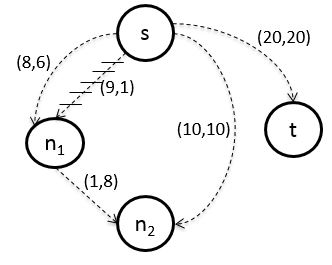
\includegraphics[width=0.4\textwidth]{Images/Chapter5/naive-pruning-example}
\caption{A pruning rule prunes a path to $n_1$ with cost (9,1) leading to the expansion of the dominated label (10,10) in $n_2$.}
\label{fig:5-1}
\end{figure} 

So we must formally show that the additional rules of \lexgo \ guarantee that only a subset of the labels expanded by \namoa \ are actually considered. To do so, Lemma \ref{lema:pruning1} analyzes the relation between pruning, goal, and Pareto preferences. Then, Theorem \ref{teo:subset} proves the desired efficiency of \lexgo, and finally, Theorem \ref{chapFormalAnalysis:teo:lexgo-admissible} establishes its admissibility.

\begin{lema}\label{lema:pruning1} 
Assume $\vec{\epsilon} \succeq \vec{0}$. Then

a) If $\vec{y} \prec_{P} \vec{y'}$  then $\vec{y} + \vec{\epsilon} \prec_{G} \vec{y'} + \vec{\epsilon}$.

b) If $\vec{y} \prec_{P} \vec{y'}$  then $\vec{y} + \vec{\epsilon} \prec_{P} \vec{y'} + \vec{\epsilon}$.

c) If $\vec{y} \prec_{P} \vec{y'}$ and $\vec{y'} \prec \vec{y''}$, then $\vec{y} \prec_{P} \vec{y''}.$

\end{lema}

\begin{demo}
Notice that, by definition,

\begin{equation}
\delta_i(\vec y, \vec{y'}) = 0 \quad \Rightarrow \quad \forall k \in I_i \hspace{3mm} s_k \geq s'_k
\label{eq:lexgo-pruning-a}
\end{equation}

Additionally, assume $d_i(\vec y) = d_i(\vec{y'})$. Since $\vec y$ has greater or equal slack than $\vec{y'}$ for all goals in level $i$, then it is straightforward that,

\begin{equation}
\forall \vec{\epsilon} \succeq \vec{0}, \quad d_i(\vec{y'} + \vec{\epsilon}) \geq  d_i(\vec{y} + \vec{\epsilon})
\label{eq:lexgo-pruning-b}
\end{equation}

Notice again that, by definition, 

\begin{equation}
\delta_j(\vec y, \vec{y'}) < d_j(\vec{y'}) - d_j(\vec{y}) \quad \Rightarrow \quad \forall \vec{\epsilon} \succeq \vec{0}, \quad d_j(\vec{y'} + \vec{\epsilon}) >  d_j(\vec{y} + \vec{\epsilon})
\label{eq:lexgo-pruning-c}
\end{equation}

Property (a) follows then from the definition of goal preferences. Assume $\vec{y} \prec_{P} \vec{y'}$, and that $\exists j \quad d_j(\vec y) < d_j(\vec{y'}) \land (\forall i < j \quad d_i(\vec y) = d_i(\vec{y'}))$. 
Then, from equations \ref{eq:lexgo-pruning-b} and \ref{eq:lexgo-pruning-c}, $\vec{y'} + \vec{\epsilon}$  will not have better deviation over $\vec{y} + \vec{\epsilon}$ for any of the first $j$ levels, and will have strictly worse deviation for at least one of them, i.e. $\vec{y} + \vec{\epsilon} \prec_{G} \vec{y'} + \vec{\epsilon}$.

For part (b) we still have to prove the additional constraints imposed on cross-slacks. Let us denote by $s''_k$ and $s'''_k$ the slack for goal $k$ of vectors $\vec{y} + \vec{\epsilon}$ and $\vec{y'} + \vec{\epsilon}$ respectively. For all levels $i<j$ we have,
\begin{align*}
\delta_i(\vec y, \vec{y'}) = 0 \quad \Rightarrow \quad \forall k \in I_i \ s_k \geq s'_k \ \ \Rightarrow \ \ \forall k \in I_i \hspace{3mm} s''_k \geq s'''_k \ \ \Rightarrow \ \ \delta_i(\vec y + \vec{\epsilon}, \vec{y'}+ \vec{\epsilon}) = 0
\label{eq:lexgo-pruning-f}
\end{align*}

\noindent and also $d_i(\vec {y'} + \vec{\epsilon}) \geq d_i(\vec {y}+ \vec{\epsilon})$. 

If for some $m < j$ \ \ $d_m(\vec {y'} + \vec{\epsilon}) > d_m(\vec {y}+ \vec{\epsilon})$, then $\delta_m(\vec y + \vec{\epsilon}, \vec{y'}+ \vec{\epsilon}) = 0 < d_m(\vec {y'} + \vec{\epsilon}) - d_m(\vec {y}+ \vec{\epsilon})$, and the property holds. Otherwise, we need to prove that the condition on cross-slacks still holds for level $j$. Let us define $\delta^i(\vec{y}, \vec{y'}) = w_i \times \max(0, s'_i - s_i)$. The following is an alternate definition of formula \ref{eq:slack-var},
\begin{align*}
    \delta_j(\vec{y}, \vec{y'}) = \sum_{m\in I_j} \delta^m(\vec{y}, \vec{y'})
 \end{align*}
	
Analogously, let us define $d^i(\vec{y}) = w_i \times \max(0, y_i - t_i)$. Then,
\begin{align*}
    d_j(\vec{y}) = \sum_{m\in I_j} d^m(\vec{y})
\end{align*}
	
Now, we analyze for each goal $m \in I_j$ its influence in deviations and cross-slack. We have three cases to consider:

\begin{itemize}
	\item When $s_m = s'_m$, deviations increase in the same amount (i.e. their relative difference does not change) and $\delta^m(\vec{y}+ \vec{\epsilon}, \vec{y'}+ \vec{\epsilon}) = \delta^m(\vec{y}, \vec{y'}) = 0$.

	\item If $s_m > s'_m$, then $d^m(\vec{y'}) - d^m(\vec{y}) \leq d^m(\vec{y'} + \vec \epsilon) - d^m(\vec{y} + \vec \epsilon)$, i.e. the relative difference between deviations can never decrease. Since $\delta^m(\vec{y}, \vec{y'}) = \delta^m(\vec{y}+ \vec{\epsilon}, \vec{y'}+ \vec{\epsilon})$ , the condition will hold for the goal.

	\item If $s_m < s'_m$, then we have to consider three distinct cases:
	\begin{itemize}
		\item When $0 \leq \epsilon_m \leq s_m < s'_m$, both deviations are zero, their relative difference remains zero and $\delta^m(\vec{y},\vec{y'})$ does not change.
		\item When $ s_m < \epsilon_m \leq s'_m$, we have $[d^m(\vec{y'}) - d^m(\vec{y}) ] - [d^m(\vec{y'} + \vec\epsilon) - d^m(\vec{y} + \vec\epsilon)] = w_m \times (\epsilon_m - s_m)$. However, we also have $\delta^m(\vec{y},\vec{y'}) - \delta^m(\vec{y} + \vec\epsilon,\vec{y'}+ \vec\epsilon) = w_m \times (\epsilon_m - s_m)$, i.e. it decreases in the same amount as before, and the inequality still holds for goal $m$. 
		\item When $ s_m  < s'_m < \epsilon_m$, we have $[d^m(\vec{y'}) - d^m(\vec{y}) ] - [d^m(\vec{y'} + \epsilon) - d^m(\vec{y} + \epsilon)] = w_m \times (s'_m - s_m)$. However, $\delta^m(\vec{y},\vec{y'}) - \delta^m(\vec{y} + \vec\epsilon,\vec{y'}+ \vec\epsilon) = w_m \times (s'_m - s_m)$, i.e. it also decreases in the same amount as before, and the inequality still holds for goal $m$. 
		\end{itemize}
\end{itemize}

Part (c) is quite straightforward. Notice that,
\begin{equation}
\vec{y'} \prec \vec{y''}  \Rightarrow  \forall l \forall k \in I_l \quad s'_k \geq s''_k
\label{eq:lexgo-pruning-d}
\end{equation}
If  $\vec{y} \prec_{P} \vec{y'}$, then we have that for all levels $i<j$, $\delta_i(\vec y, \vec{y'}) = 0$, 
$\delta_i(\vec y, \vec{y''}) = 0$, and $d_i(\vec{y''}) \geq d_i(\vec{y'}) = d_i(\vec{y})$. 

Let us examine level $j$. From equation \ref{eq:lexgo-pruning-d} it follows that $\delta_j(\vec y, \vec{y'}) \geq \delta_j(\vec y, \vec{y''})$ and from dominance $d_j(\vec{y''}) \geq d_j(\vec{y'})$. In consequence,

\begin{equation}
d_j(\vec{y''}) - d_j(\vec{y}) \  \geq \ d_j(\vec{y'}) - d_j(\vec{y}) \ > \ \delta_j(\vec y, \vec{y'}) \  \geq \ \delta_j(\vec y, \vec{y''})
\label{eq:lexgo-pruning-e}
\end{equation}

\noindent and therefore $\vec{y} \prec_{P} \vec{y''}$. $\Box$

\end{demo}

\begin{teorema}\label{teo:subset}
When the lower bound function is monotone \lexgo \ explores a subset of the labels explored by \namoa, i.e. if \namoa \ does not explore a label $(n, \vec g)$, \lexgo \ will not explore it either.
\end{teorema}

\begin{demo}
A label $(n, \vec g, \vec f)$ is not explored by \namoa \ if (a) $\exists \vec{c^*} \in C^*$ such that $\vec{c^*} \prec \vec f$, or (b) $\vec g$ is dominated in $n$. 

It is straightforward that \lexgo \ never explores a label discarded by  \namoa \ by condition (a). Since  $C^*_G \subseteq C^*$, for all $c^* \in C^*$, either $c^* \in C_G^*$, or $\vec d_B = \vec{d^*} \prec_L \vec d(\vec{c^*})$. In the latter case, if for some $\vec f$, $\vec{c^*} \prec \vec f$, then $\vec{d^*} \prec_L \vec d(\vec{c^*}) \preceq_L \vec d(\vec f)$. Therefore, \lexgo \ filters the labels with equations \ref{eq:cond-filter-dom} and \ref{eq:cond-filter-new}.  

Let us consider now labels discarded by \namoa \ by condition (b). Let us assume a non-dominated path $P = (s, n, \ldots, n_i, \ldots, n_k)$ to $n_k$ represented by label $(n_k, \vec g, \vec f)$, and its two subpaths $P_1 = (s, n, \ldots, n_i)$ and $P_2 = (n_{i+1}, \ldots, n_k)$. Let us also assume a dominated path $P' = (s, \ldots, n_k)$ to $n_k$ in OPEN with label $(n_k, \vec{g'}, \vec{f'} )$.  Finally, lets assume that $P_1$ is the largest subpath of $P$ to enter OPEN, with label $(n_i, \vec g_1, \vec f_1)$. This situation is depicted in  Figure \ref{fig:4-2-prune}.

Let us assume label $(n_i, \vec g_1, \vec f_1)$ is in OPEN. Since the lower bound function is monotone, as defined in the assumptions, \ $\vec g_1 + \vec h_i \preceq \vec g + \vec h_k \prec \vec{g'} + \vec h_k$ and $P'$ can never be selected by \lexgo. If eventually, $n_i = n_k$ $P'$ is dominated and pruned by $P$.

On the other hand, if $(n_i, \vec g_1, \vec f_1)$ is never selected and not in OPEN, then there must be some other path $P_3$ that pruned $P_1$, i.e. $\vec f(P_3) \prec_P \vec f(P_1)$. By Lemma \ref{lema:pruning1}(b), we have $\vec f(P_3P_2) \prec_P \vec f(P_1P_2)$. This fact, together with the fact that $\vec f(P_1P_2) \prec \vec f(P')$, leads us to conclude by virtue of Lemma \ref{lema:pruning1}(c), that  $\vec f(P_3P_2) \prec_P \vec f(P')$, i.e. if a path prunes some other non-dominated path, then the extensions of the former will also prune those that would be pruned by the latter. Therefore, the property holds.$\Box$  

\begin{figure}[!ht]
\centering
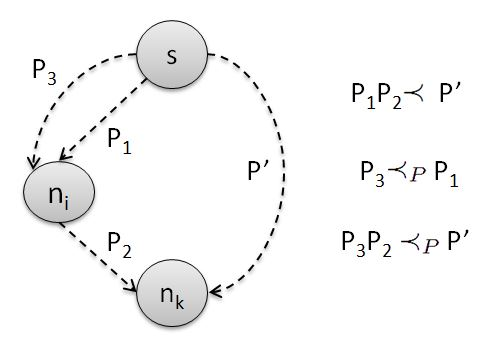
\includegraphics[width=0.4\textwidth]{Images/Chapter5/prune}
\caption{Scenario where a dominated path $P'$ is pruned either by $P_1P_2$ or $P_3P_2$.}
\label{fig:4-2-prune}
\end{figure} 

\end{demo}

%-------------------------------------------------------------------
\subsection{Admissibility}
\label{chapFormalAnalysis:sec:admissibilityLexgo}  
%-------------------------------------------------------------------

Once the efficiency of \lexgo \ has been established, we turn our attention to admissibility, i.e. to prove that the subset of labels explored by \lexgo \ still includes all goal-optimal solutions. A scalar algorithm is said to be \emph{admissible} if it is guaranteed to return an optimal solution whenever a solution exists. We extend the definition as follows: a multiobjective search algorithm with goal-based preferences is \emph{admissible} if it terminates with the set of \emph{all} goal-optimal solutions to the problem. 

\begin{teorema} \label{chapFormalAnalysis:teo:lexgo-admissible}
Algorithm \lexgo \ is admissible.
\end{teorema}

\begin{demo}
\lexgo \ is a label-setting algorithm that generates partial paths from the start node to the destination. Each partial path is either expanded, filtered, or pruned. A goal-optimal solution could be pruned by pruning conditions \ref{eq:cond-prune-dom} or \ref{eq:cond-prune-deviation} as described in Section \ref{subsubsec:Pruning-conditions}, or could be filtered by filtering conditions \ref{eq:cond-filter-dom} or \ref{eq:cond-filter-new} from Section \ref{subsubsec:Filtering-conditions}. By definition, a goal-optimal solution has a non-dominated cost. Since the optimality principle holds for dominated costs, neither pruning condition \ref{eq:cond-prune-dom} nor filtering condition \ref{eq:cond-filter-dom} will ever discard a goal-optimal solution.

The proof for condition \ref{eq:cond-prune-deviation} follows. Let us assume two paths $P^1=(s,\ldots,n)$ and $P^2=(s,\ldots,n)$, leading to the same node $n$, and an additional Pareto-optimal path $P^3 =(n,\ldots,t)$ leading from $n$ to a destination node. Let us call $\vec{f^1} = \vec{f}(P^1) = \vec g(P^1) + \vec{h}(n)$, 
$\vec{f^2} = \vec{f}(P^2) = \vec g(P^2) + \vec{h}(n)$.
Since the lower bound is optimistic, we know that $\vec{h}(n) \preceq \vec g(P^3)$. Let us call $\vec{e} = \vec g(P^3) - \vec{h}(n) \succeq \vec{0}$.
Extending $P^1$ and $P^2$ with $P^3$, the costs of both solutions are
respectively $\vec{f^{13}}= \vec g(P^1) + \vec g(P^3) = \vec g(P^1) + \vec{h}(n) + \vec{e} = \vec{f^1} + \vec{e}$ \ and $\vec{f^{23}}= \vec g(P^2) + \vec g(P^3) = \vec g(P^2) + \vec{h}(n) + \vec{e} = \vec{f^2} + \vec{e}$.

Let us assume that $P^1$ prunes $P^2$ in virtue of condition \ref{eq:cond-prune-deviation}. Then $\vec{f^1} \prec_P\vec{f^2}$ and, by Lemma \ref{lema:pruning1}(a), $\vec{f^{13}} = \vec{f^1} + \vec{e} \prec_G \vec{f^2} + \vec{e} = \vec{f^{23}}$, so by this expansion $P^2$ does not lead to a better solution than $P^1$. Since no assumptions were made about $P^3$, the result holds for every expansion of $n$, therefore $P^2$ does not lead to a better solution than $P^1$ and the pruning is correct.

Finally, let us consider filtering condition \ref{eq:cond-filter-new}, due to the lexicographic selection policy, the deviation of the first solution found $\bestd = \vec d_t$ is trivially equal or lexicographically better than the deviation of any other label in OPEN. No goal-optimal solution cost $\vec{c^*} \in C_G^*$ with deviation $\vec d(\vec{c^*})$ can have worse lexicographical deviation than $\bestd$
%, $\bestd \nprec_L \vec d(\vec{c^*})$, otherwise $\vec g_t \prec_G \vec{c^*}$ and it could not be a goal-optimal solution. 
Therefore, filtering condition \ref{eq:cond-filter-new} never filters goal-optimal solutions.

Since \lexgo \ never prunes nor filters goal-optimal solutions, the only remaining possibility is that they are all selected and found before termination, i.e. \lexgo \ is admissible.$\Box$
\end{demo}

%-------------------------------------------------------------------
\section{Formal characterization of \texorpdfstring{\namoate}{NAMOA*te}}
\label{chapFormalAnalysis:sec:analysisNAMOATE}
%-------------------------------------------------------------------

This section proves some relevant properties of \namoate \ under reasonable assumptions. The t-discarding method, see Section \ref{chapMultiObjAlg:sec:Time-efficient-MSalg}, introduces a new technique to check dominance of new alternatives against the solutions already found (filtering) and against partial paths to each node already explored (cl-pruning). We will show that \namoa \ is not affected when the t-discarding technique is applied instead of the standard dominance tests. 

%-------------------------------------------------------------------
\subsection{Admissibility}
\label{chapFormalAnalysis:sec:admissibilityNamoate}
%-------------------------------------------------------------------

In order to demonstrate the admissibility of \namoate, we will make the following assumptions:

\begin{supo} \label{supo:1}
The lower bound function returns a single vector estimate for each node, i.e. $H(n) = \{  \vec h(n) \}$, and satisfies the monotone property.
\end{supo}
Assumption \ref{supo:1} is satisfied by the precalculated lower bound proposed by Tung and Chew \citep{Tung1992}, which corresponds to the ideal point. This single-valued multiobjective lower bound has been shown to be very effective in practice \citep{Machuca2011b}.


\begin{supo} \label{supo:2}
The lexicographic order is applied to select non-dominated labels
from OPEN, that is, if $(n,\vec g,\vec f)$ is selected, then for all $(n',\vec{g'},\vec{f'})\in$ OPEN, $\vec f \preceq_L \vec{f'}$. 
\end{supo}

Lexicographic order is a common choice in multiobjective search algorithms, since the lexicographic optimum is also non-dominated. Notice that dominance always implies lexicographical preference, that is,
if $\vec x \prec \vec y$ then $\vec x \prec_L \vec y$, and if $\vec x \preceq \vec y$ then $\vec x \preceq_L \vec y$
(obviously the opposite is not true).

%Notice that another selection order could also be employed as long as the first vector component is monotone nondecreasing, i.e. $f_1 \leq f'_1$.

We  will prove (Theorem \ref{teo:teo}) that under Assumptions \ref{supo:1} and \ref{supo:2}
\namoate \ is not affected when filtering and cl-pruning use t-discarding checks instead of standard dominance checks.
We will prove first two auxiliary results (Lemmas \ref{lema:lex} and \ref{lema:truncated-pruning}).

Let $\vec v$ be a vector and $X$ a set. We will write $X\preceq_L \vec v$ when $\vec v$ is an upper lexicographic bound of $X$, that is, when
for every $\vec{v'}\in X$, $\vec{v'}\preceq_L \vec v$.  

\begin{lema}\label{lema:lex}
Given Assumptions \ref{supo:1} and \ref{supo:2}, when a label $l = (n,\vec g,\vec f)$ is selected from OPEN, then (i) $G_{cl}(n) \preceq_L \vec g$; and (ii) COSTS $\preceq_L \vec f$.
\end{lema}

\begin{demo}
Let us define OPEN$_t$ as the set of open labels at iteration $t$ and assume $(m,\vec{g'},\vec{f'})$ was selected at iteration $t$ of the algorithm. 
Then, at that moment, for all $(n'',\vec{g''},\vec{f''}) \in $ OPEN$_t$
we have (by Assumption \ref{supo:2}) $\vec{f'}\preceq_L \vec{f''}$.
Let us consider now the label $(n, \vec g, \vec f)$ selected from OPEN$_{t+1}$ at the next iteration $t+1$.
If it was already $(n, \vec g, \vec f) \in $ OPEN$_t$, then obviously $\vec{f'} \preceq_L \vec f$.
If $(n, \vec g, \vec f)$ is a new label, then $n$ is a child of $m$ and $\vec g = \vec{g'} + \vec c(m,n)$.
By Assumption  \ref{supo:1}, $\vec h(m) \preceq \vec c(m,n) + \vec h(n)$ and hence
$\vec{f'} = \vec{g'} + \vec h(m) \preceq \vec{g'} + \vec c(m,n) + \vec h(n) = \vec g + \vec h(n) = \vec f$ 
and hence $\vec{f'} \preceq_L \vec f$. We have proved that 
if $(m,\vec{g'},\vec{f'})$ is selected for expansion at iteration $t$ and $(n, \vec g, \vec f)$ at iteration $t+1$ then $\vec{f'}\preceq_L \vec f$; and 
it trivially follows by induction that if $(m,\vec{g'},\vec{f'})$ is selected for expansion before $(n, \vec g, \vec f)$ then $\vec{f'}\preceq_L \vec f$.

Now we can prove part (i) of the lemma. Let us consider the set $G_{cl}(n)$. 
If $\vec{g'}\in G_{cl}(n)$, then there is a closed label $(n,\vec{g'},\vec{f'})$ at $n$ that was selected before $(n,\vec g,\vec f)$, so $\vec{f'}\preceq_L \vec f$. Since $\vec f = \vec g + \vec h(n)$ and $\vec{f'} = \vec{g'} + \vec h(n)$, then $\vec{g'}\preceq_L \vec g$, so $G_{cl}(n)\preceq_L \vec g$ as stated in part (i).

Let us consider now the set COSTS. If $\vec{f'}\in$ COSTS, it belongs to a label
$(\gamma, \vec{f'},\vec{f'})$ (where $\gamma$ is the destination node) that has been already selected, so $\vec{f'}\preceq_L \vec f$, as stated in part (ii).  $\Box$
\end{demo}

\begin{lema}\label{lema:truncated-pruning} 
Let $\vec v$ be a vector and $X$ a set of vectors such that $X \preceq_L \vec v$.
Then $\vec v$ is dominated by $X$ iff $\vec v$ is t-discarded by $X$. 
\end{lema}

\begin{demo}
The ``if'' direction is trivial: if  $\vec v$ is t-discarded by $X$,
both condition (a) and condition (b) in Definition \ref{chapMultiObjAlg:def:tv3} imply that there exists $\vec{v'}\in X$
such that $\vec{v'} \prec v$, hence $\vec v$ is dominated by $X$.

The ``only if'' direction is also immediate:
Suppose $\vec v$ is dominated by $X$. Then there exists at least a $\vec{v'}\in X$ 
such that $\vec{v'}\prec v$. Suppose first that $t(\vec{v'})\in T(X)$ and
$v'_1 < v_1$. Then it must be $t(v'_1) \preceq t(v_1)$.
So $\vec{v'}$ satisfies conditions imposed in Definition \ref{chapMultiObjAlg:def:tv3} (option a)
to t-discard $\vec v$. On the other hand, if  $v'_1 = v_1$  it must be $t(\vec{v'}) \prec t(\vec v)$
and $v'$ also satisfies conditions imposed in Definition \ref{chapMultiObjAlg:def:tv3} (option b).
Let us suppose now $t(\vec{v'})\notin T(X)$. Then $t(\vec{v'})$ is dominated by a certain $t(\vec{v''})$,
that is, $t(\vec{v''}) \prec t(\vec{v'}) \preceq t(v)$.
And, since $\vec{v''}\in X \preceq_L \vec v$, it must be $v''_1 \leq v_1$. But if $v''_1 < v_1$,
$\vec{v''}$ allows to t-discard $\vec v$ (option a); and if $v''_1 = v_1$,
$\vec{v''}$ allows to t-discard $\vec v$ (option b).
So, in any case, if $\vec v$ is dominated by $X$ then $\vec v$ is t-discarded by $X$. $\Box$
\end{demo}

\begin{teorema}\label{teo:teo}
Under Assumptions \ref{supo:1} and \ref{supo:2}, the workings of \namoa \ are unaffected if filtering and/or cl-pruning  
are defined as follows:

\begin{itemize}
    \item Filtering. Discard $(n,\vec g,\vec f)$ if $\vec f$ is t-discarded by COSTS.
	 \item Cl-pruning. Discard $(n,\vec g,\vec f)$ if $\vec g$ is t-discarded by $G_{cl}(n)$.
\end{itemize}

\end{teorema}

\begin{demo}
First note that by Lemma \ref{lema:lex} when a label $l = (n,\vec g,\vec f)$ is selected from OPEN, then $G_{cl}(n)\preceq_L \vec g$ and COSTS $\preceq_L \vec f$. Lemma \ref{lema:truncated-pruning} guarantees in that case that dominance and t-discarding by a set $X$ are equivalent. So, a new label will be cl-pruned and/or filtered exactly in the same cases. $\Box$
\end{demo}

%-------------------------------------------------------------------
\subsection{Efficiency}
\label{chapFormalAnalysis:sec:efficiencyNamoate}
%-------------------------------------------------------------------

The real advantage of t-discarding is time performance. A recent work \citep{Mandow2009} shows that when arc costs are integer in the interval $[c_i,c_a]$, $c_i,c_a > 0$, then the worst-case number of Pareto optimal costs reaching a node at depth $d$ with $q$ objectives is $O((dr)^{q-1})$, where $r= c_a - c_i + 1$. This is, therefore, a worst-case bound on the size of the COSTS and $G_{cl}(n)$ sets, and in the number of dominance checks against those sets.

The use of t-discarding implies checking only against the $T(\text{COSTS})$ and $T(G_{cl}(n))$ sets. The size of vectors in these sets is $q' = q - 1$, hence the worst-case size of the $T(\text{COSTS})$ and $T(G_{cl}(n))$ sets is only $O((dr)^{q-2})$.

Let us consider the class of problems with three objectives ($q=3$). Then, the worst-case size of the $G_{cl}(n)$ and COSTS sets grows quadratically with depth and range of costs (and so does the worst-case number of dominance comparisons). However, with t-dominance this growth is limited to a linear case. The next chapter presents a set of experiments to evaluate the effectiveness of this method in practice.

%-------------------------------------------------------------------
\section{Formal characterization of \texorpdfstring{\lexgote}{LEXGO*te}}
\label{chapFormalAnalysis:sec:analysisLexgote}
%-------------------------------------------------------------------

This section analyzes the applicability of the t-discarding technique to \lexgo. t-discarding requires evaluation vectors $\vec f$ to be selected in lexicographical order by the algorithm. This is easy to achieve for multiobjective search with a lexicographical policy, but cannot be straightforwardly applied in goal-based search, due to goal-based search with a lexicographical selection order selects the lexicographical optimal deviation vector, not the lexicographical optimal non-dominated f-vector (like in multiobjective search). An scenario where t-discarding can be applied to \lexgo \ preserving its admissibility follows.

%-------------------------------------------------------------------
\subsection{Admissibility}
\label{chapFormalAnalysis:sec:admissibilityLexgote}
%-------------------------------------------------------------------

\begin{supo} \label{supo:3}
The lexicographic order is applied to select goal-optimal labels
from OPEN, that is, if $(n,\vec g,\vec f,\vec d)$ is selected, then for all $(n',\vec{g'},\vec{f'},\vec{d'})\in$ OPEN,
$\vec d \preceq_L \vec{d'}$ and if $\vec d = \vec{d'}$ then $\vec f \preceq_L \vec{f'}$. 
\end{supo}
 
By definition of a goal-optimal solution, the lexicographically optimal deviation vector according to the concatenation of deviation and estimate vectors, $\vec d \cdot \vec f$, is a goal-optimal alternative, i.e. it has a non-dominated deviation and it is a non-dominated vector.

\begin{lema}\label{lema:lexgote}
Given Assumptions \ref{supo:1} and \ref{supo:3}, when a label $l = (n,\vec g,\vec f,\vec d)$ is selected from OPEN and  $\vec d = \vec 0$ then for all $(\vec{g'},\vec{f'},\vec{d'})\in$ OPEN, $\vec d \cdot \vec f \preceq_L \vec{d'} \cdot \vec{f'}$ and (i) $G_{cl}(n) \preceq_L \vec g$; and (ii) COSTS $\preceq_L \vec f$.
\end{lema}

\begin{demo}
On one hand, when $\vec d = \vec 0$, obviously, for all $(n',\vec{g'},\vec{f'},\vec{d'})\in G_{cl}(n)$, $ \vec{d'} = \vec 0$ and in a similar way to Lemma \ref{lema:lex}, we can remove d-vectors and achieve the same result, i.e.  $G_{cl}(n) \preceq_L \vec g$.

On the other hand, if $ \vec d = \vec 0$ and $l$ is selected from OPEN, if there exists any $\vec{c^*} \in$ COSTS, by definition, $d(\vec{c^*}) = \vec 0$. Therefore, in an equivalent way to Lemma \ref{lema:lex}, we can remove d-vectors and achieve the same result, i.e. COSTS $\preceq_L \vec f$. $\Box$
\end{demo}

\begin{teorema}\label{teo:teo-lexgote}
Under Assumptions \ref{supo:1} and \ref{supo:3}, the workings of \lexgote \ are unaffected if filtering and/or cl-pruning are defined as follows:

\begin{itemize}
    \item Filtering. Discard $(n, \vec g, \vec f, \vec d)$ if $\vec f$ is t-discarded by COSTS.
	 \item Cl-pruning. Discard $(n, \vec g, \vec f, \vec d)$ if $\vec g$ is t-discarded by $G_{cl}(n)$.
\end{itemize}

\end{teorema}

\begin{demo}
The same argument used in Theorem \ref{teo:teo} applies to prove that dominance and t-discarding by a set $X$ are equivalent in \lexgote \ when a  label $l = (n, \vec g, \vec f, \vec d)$ with $\vec d= \vec 0$ is selected from OPEN. Thus, this new label will be cl-pruned and/or filtered exactly in the same cases for \lexgote \ as it was in \lexgo. $\Box$
\end{demo}

%-------------------------------------------------------------------
\section{Discussion}
\label{chapFormalAnalysis:sec:discussion}
%-------------------------------------------------------------------

This section has reviewed the formal properties of \namoa, and presented some analogous properties for the three algorithms introduced in this thesis. More precisely, the admissibility (i.e. the exactness of the algorithms) is formally proved for all of them and their relative efficiency is also examined.

\namoa \ is known to be optimal in the number of path expansions among the class of admissible best-first algorithms when using consistent lower bounds. \lexgo \ has also been proven to be admissible. 

The worst case scenario for \lexgo \ is when the whole Pareto set of solutions satisfies the goals. The important theoretical results showed in this chapter indicate that (a) provided with the same lower bounds, \lexgo \ always expands a subset of the labels expanded by \namoa ; (b) the superiority in runtime of \namoate \ over \namoa ; and (c) the superiority in runtime of \lexgote \ over \lexgo. These important theoretical results do not completely settle the question of which algorithm is better in practice. We address a comprehensive empirical analysis of this question in Chapters \ref{chapEmpiricalAnalysisGrids} and \ref{chapEmpiricalAnalysisRoadMaps}.

%Chapters \ref{chapEmpiricalAnalysisGrids} and \ref{chapEmpiricalAnalysisRoadMaps} present a detailed empirical analysis of the four algorithms employing different selection order policies. The comparisons are carried out in pairs, in order to define the relative performance between each pair of similar algorithms with and without the improvement added.

%---------------------------------------------------------------------
%
% Chapter 6: Empirical Analysis On Grid Problems
%
%---------------------------------------------------------------------
%
% ChapEmpiricalAnalysisGrids.tex
% Copyright 2015 Dr. Francisco J. Pulido
%
% This file belongs to the PhD titled "New Techniques and Algorithms for Multiobjective and Lexicographic Goal-Based Shortest Path Problems", distributed under the Creative Commons Licence Attribution-NonCommercial-NoDerivs 3.0, available in http://creativecommons.org/licenses/by-nc-nd/3.0/. The complete PhD dissertation is freely accessible from http://www.lcc.uma.es/~francis/
%
% This thesis has been written adapting the TeXiS template, a LaTeX template for writting thesis and other documents. The complete TeXiS package can be obtained from http://gaia.fdi.ucm.es/projects/texis/. TeXis is distributed under the same conditions of the LaTeX Project Public License (http://www.latex-project.org/lppl.txt). The complete license is available in http://creativecommons.org/licenses/by-sa/3.0/legalcode
%
%---------------------------------------------------------------------

\chapter{Empirical Analysis on Grid Problems}
\label{chapEmpiricalAnalysisGrids}
%
\begin{FraseCelebre}
\begin{Frase}
It doesn't matter how beautiful your theory is, it doesn't matter how smart you are. If it doesn't agree with experiment, it's wrong.
\end{Frase}
\begin{Fuente}
Richard P. Feynman (1918-1988)
\end{Fuente}
\end{FraseCelebre}
%
%\begin{resumen}
%

One of the main goals of this thesis is to develop efficient procedures for the goal-based search problem. In Chapter \ref{chapContributions} we introduced \lexgo, a new search algorithm for lexicographic goal problems, as well as an improved procedure for efficient dominance checks in multicriteria search algorithms. This procedure can be applied to \lexgo \ and \namoa, yielding algorithms \lexgote \ and \namoate. Formal properties of these algorithms were presented in Chapter \ref{chapFormalAnalysis}. \lexgo \ and \lexgote \ always return the set of all goal-optimal solutions to a lexicographic goal search problem, while \namoate \ returns the set of all Pareto-optimal solutions to a Multiobjective Search Problem.

In this chapter we evaluate experimentally the performance of two different strategies for lexicographic goal problems: (a) use a multiobjective search algorithm (like \namoa \ or \namoate), and then select the goal-optimal solutions among those in the Pareto set, (b) use a specific goal-based algorithm (like \lexgo \ or \lexgote).

First, we shall describe the experimental setup in Section \ref{chapEmpiricalAnalysis:sec:grids}, which is based on the use of randomly generated grid problems with three to five criteria. We analyze time and space performance of the algorithms for problems of increasing depth. We also evaluate performance for different kinds of goal preferences. More precisely, we set up goals that range from unsatisfiability to satisfability by increasingly larger subsets of the Pareto set. Chapter \ref{chapEmpiricalAnalysisRoadMaps} will present additional experiments over route planning problems in realistic road maps.

We perform systematic comparisons between the algorithms. First we compare \lexgo \ against full Pareto search with \namoa \ (using both lexicographic and linear aggregation selection policies in both algorithms) in Section \ref{chapEmpiricalAnalysis:sec:resultsgridslexgo}. Then, we evaluate the algorithms that employ the dimensionality reduction technique against the standard ones. First, we compare in Section \ref{chapEmpiricalAnalysis:sec:resultsgridsnamoate} \namoa \ with a linear aggregation selection policy against our new version \namoate. After that we compare \lexgote \ against \lexgo \ in Section \ref{chapEmpiricalAnalysis:sec:resultsgridslexgote}. Finally, we evaluate both versions that employ t-discarding over problems with goals. A summary and conclusions are presented at the end of this chapter.

%-------------------------------------------------------------------
\section{Experimental setup}
\label{chapEmpiricalAnalysis:sec:grids}
%-------------------------------------------------------------------

This chapter evaluates the performance of algorithms over sets of randomly generated grids. Furthermore, we have generated three uncorrelated criteria in order to evaluate search with goal-based preferences and three to five uncorrelated criteria when we evaluate multiobjective search without preferences (\namoa \ versus \namoate). The solution depth is used as an indicator of problem difficulty. All multiobjective search algorithms analyzed in this thesis employ the ideal point as lower bound (described in Section \ref{chapMultiObjAlg:subsec:tc}). 

We use randomly generated grids which are a standard test bed in the evaluation of multicriteria search algorithms \citep{Machuca2012} \citep{Raith2009a}. Square bi-dimensional grids of $100 \times 100$ nodes with a vicinity of four neighbors were generated as described in Section \ref{chapMultiObjTestBeds:subsec:RandomGrids}. The start node is placed at the grid center and a single destination node is placed in the diagonal from the center to the bottom right corner. Different solution depths are considered, varying from 20 to 100. A set of five different problems was generated for each solution depth. For each arc a vector $\vec c(i,j) = (c_1,c_2,...,c_q)$ of $q$ integer scalar costs was randomly generated in the range [1,10] using an uniform distribution, i.e. leading to uncorrelated objectives.

In order to assess search with goal-based preferences two different classes of experiments were carried out. Three goals grouped in two priority levels were considered, where target values are defined in terms of the ideal and nadir points. The first class of experiments defines five different sets of targets using the constant $k_1 \in \{ 0, 0.25, 0.5, 0.75, 1 \}$ for both priority levels (see Equation \ref{eq:targets}). For the second class, targets of the first level are fixed for $k_1=0.75$ and $k_1=0.5$, using the constant $k_2 = k_1 \times k^\prime$ to set the targets of the second priority level, with $k^\prime \in \{ 0.25, 0.5, 0.75, 1 \}$ (see Equation \ref{eq:targets2}). The complete description regarding the generation of these classes of experiments can be seen in Section \ref{chapMultiObjTestBeds:subsec:Performance}.

Regarding multiobjective search performance, the experiments over \namoa \ and \namoate \ are carried out with three, four and five uncorrelated criteria. All solution depths for each number of criteria range from $d=20$ to the maximum solution depth by increments of 10. The maximum solutions depths considered are $d=100$, $d=50$, and $d=40$ for $q=3$, $q=4$ and $q=5$, respectively. 

This study analyzes for \namoa \ and \lexgo \ the following aspects as a function of solution depth:

\begin{enumerate}
    \item The percentage of goal-optimal solutions returned by \lexgo \ relative to the size of the full Pareto set returned by \namoa.
	 \item The percentage of scanned labels by \lexgo \ relative to the number of scanned labels by \namoa.
	 \item The relative runtime requirements of \lexgo \ to \namoa.
\end{enumerate}  

Additionally, in order to analyze the performance of the t-discarding technique 
the following aspects are analyzed as a function of solution depth:

\begin{enumerate}
    \item The size of the truncated sets of closed labels ($T(G_{cl})$) and solutions (T(COSTS)) relative to the complete sets of \namoa. 
	 \item The percentage of cl-pruned and filtered labels over the total number of discarded labels.
	 \item Time requirements of t-discarding algorithms (\namoate \ or \lexgote) relative to their reference algorithms (\namoa \ or \lexgo).
\end{enumerate}  

The algorithms were implemented to share as much code as possible. The programming language used was ANSI Common Lisp using LispWorks Professional 6.01 (64-bit). The OPEN queue of alternatives was implemented as a binary heap but only the current best estimate of each node is kept in OPEN at each iteration. The $G_{op}$ and $G_{cl}$ sets are ordered according to the label selection policy employed by the algorithm. Lexicographic and linear orders were used to choose among non-dominated open alternatives in \namoa \ and \lexgo. Their counterparts with the t-discarding technique \namoate \ and \lexgote \ employ the lexicographic order.

Grid problems were run on an Intel Core i7 3612QM at 2.1 GHz and 4 GB of DDR3 RAM. All experiments were run on a single thread.

%-------------------------------------------------------------------
\section{\texorpdfstring{\lexgo}{LEXGO*} \ vs \texorpdfstring{\namoa}{NAMOA*}}
\label{chapEmpiricalAnalysis:sec:resultsgridslexgo}
%-------------------------------------------------------------------

This section presents the comparison between \namoa \ and \lexgo. The study tested both the lexicographic and linear selection orders (see Definitions \ref{chapMultiObjAlg:def:lexorder} and \ref{chapMultiObjAlg:def:linorder} for further description of the OPEN selection orders employed in this thesis). Regarding \namoa, the first variant is called \namoalex, and uses a lexicographic order of selection. The second, called \namoalin, uses an order of selection based on a linear aggregation of vector components. Similarly, the first variant of \lexgo \ is called \lexgolex \ and the second \lexgolin. These four alternatives are evaluated over the two classes of experiments described in Section \ref{chapEmpiricalAnalysis:sec:grids}. Additionally, the performance of \lexgo \ was evaluated with and without the deviation-based pruning (see Equation \ref{eq:cond-prune-deviation}), in order to evaluate the effectiveness of this newly introduced pruning condition.

Notice that both algorithms, \namoa \ and \lexgo, return exactly the same set of solutions regardless the label selection policy, i.e. both \namoalex \ and \namoalin \ return the full Pareto set of efficient solutions to the problem, that is referred to as $C^*$, whereas \lexgolex \ and \lexgolin \ return the same set of goal-optimal solutions. Thus, the first comparison between them is devoted to analyze the percentage of goal-optimal solutions regarding the full Pareto set. Then, the space and runtime performance are analyzed. The former is measured by the relative number of scanned labels, and the latter by a runtime performance comparison when the lexicographic or the linear aggregation selection orders are employed. 

These experiments were partly published by the author and reported in \citep{Pulido2014}. The results in this thesis go beyond those experiments and also consider the linear selection order and $k_1 = 0.75$ in class II experiments. 

%-------------------------------------------------------------------
\subsection{Analysis on class I experiments}
\label{chapEmpiricalAnalysis:subsec:analysisgridslexgoc1}
%-------------------------------------------------------------------

Table \ref{tab:6-1} shows reductions in the number of Pareto-optimal solution vectors returned by \lexgo \ relative to the full Pareto set $C^*$. 
It can be observed that for large values of $k_1$ the subset of Pareto-optimal solution vectors returned by \lexgo \ is somewhat reduced. However, for $k_1=0.5$ only about $20\%$ of the Pareto set is returned. For $k_1=0.25$ or $k_1=0$, no solution satisfies all goals, and a subset of only one or two Pareto-optimal solution cost vectors minimizing deviation is returned. This is also beneficial for the efficiency of \lexgo \ since the number of computationally costly filtering checks is greatly reduced when compared to \namoa. The portion of the Pareto set returned for varying $k_1$ appears graphically illustrated in Figure \ref{fig:6-1} for a sample problem with solution depth $d=100$.

\begin{table}
\caption{Class I experiments on grids, average percentage of goal-optimal solution vectors returned by \lexgo \ relative to average $|C^*|$ as a function of  solution depth. An asterisk ($^*$) indicates that the goals could not be satisfied.}
\centering
\begin{tabular}{rrrrrrrr}
\hline \noalign{\smallskip}
& & \multicolumn{5}{c}{\lexgo} \\
\noalign{\smallskip} \cline{3-7} \noalign{\smallskip}
& \namoa & 1 & 0.75 & 0.5 & 0.25 & 0 & \multicolumn{1}{c}{$k_1$}\\
\noalign{\smallskip} 
$d$ & Avg. $|C^*|$ & \% & \% & \% & \% & \% \\
\cline{1-7}  \noalign{\smallskip} 
20 & 122 & 100 & 74.3 & 20.5 & 0.98$^*$ & 0.82$^*$ \\ 
30 & 302 & 100 & 77.6 & 22.2 & 0.33$^*$ & 0.33$^*$ \\
40 & 694 & 100 & 78.7 & 20.8 & 0.14$^*$ & 0.17$^*$ \\
50 & 1,599 & 100 & 78.2 & 16.8 & 0.06$^*$ & 0.06$^*$ \\
60 & 2,007 & 100 & 83.0 & 24.6 & 0.06$^*$ & 0.05$^*$ \\ 
70 & 2,561 & 100 & 82.4 & 24.6 & 0.04$^*$ & 0.04$^*$ \\ 
80 & 5,423 & 100 & 82.3 & 20.3 & 0.02$^*$ & 0.02$^*$ \\ 
90 & 5,912 & 100 & 77.7 & 21.0 & 0.02$^*$ & 0.03$^*$ \\ 
100 & 8,307 & 100 & 77.9 & 17.0 & 0.01$^*$ & 0.01$^*$ \\ 
\hline
\end{tabular}
\label{tab:6-1}
\end{table} 

This figure displays all Pareto-optimal solution vectors in cost (or attribute) space. The figure displays a box enclosing all Pareto-optimal solution vectors, delimited by the ideal and nadir points $(k_1 = 1)$. Boxes delimiting the regions of cost space that would satisfy the goals established by parameter $k_1$  equal to 0.75, 0.5 and 0.25 are also displayed. In the case $k_1 = 0$ only the ideal point would satisfy the goals.

\begin{figure}
\centering
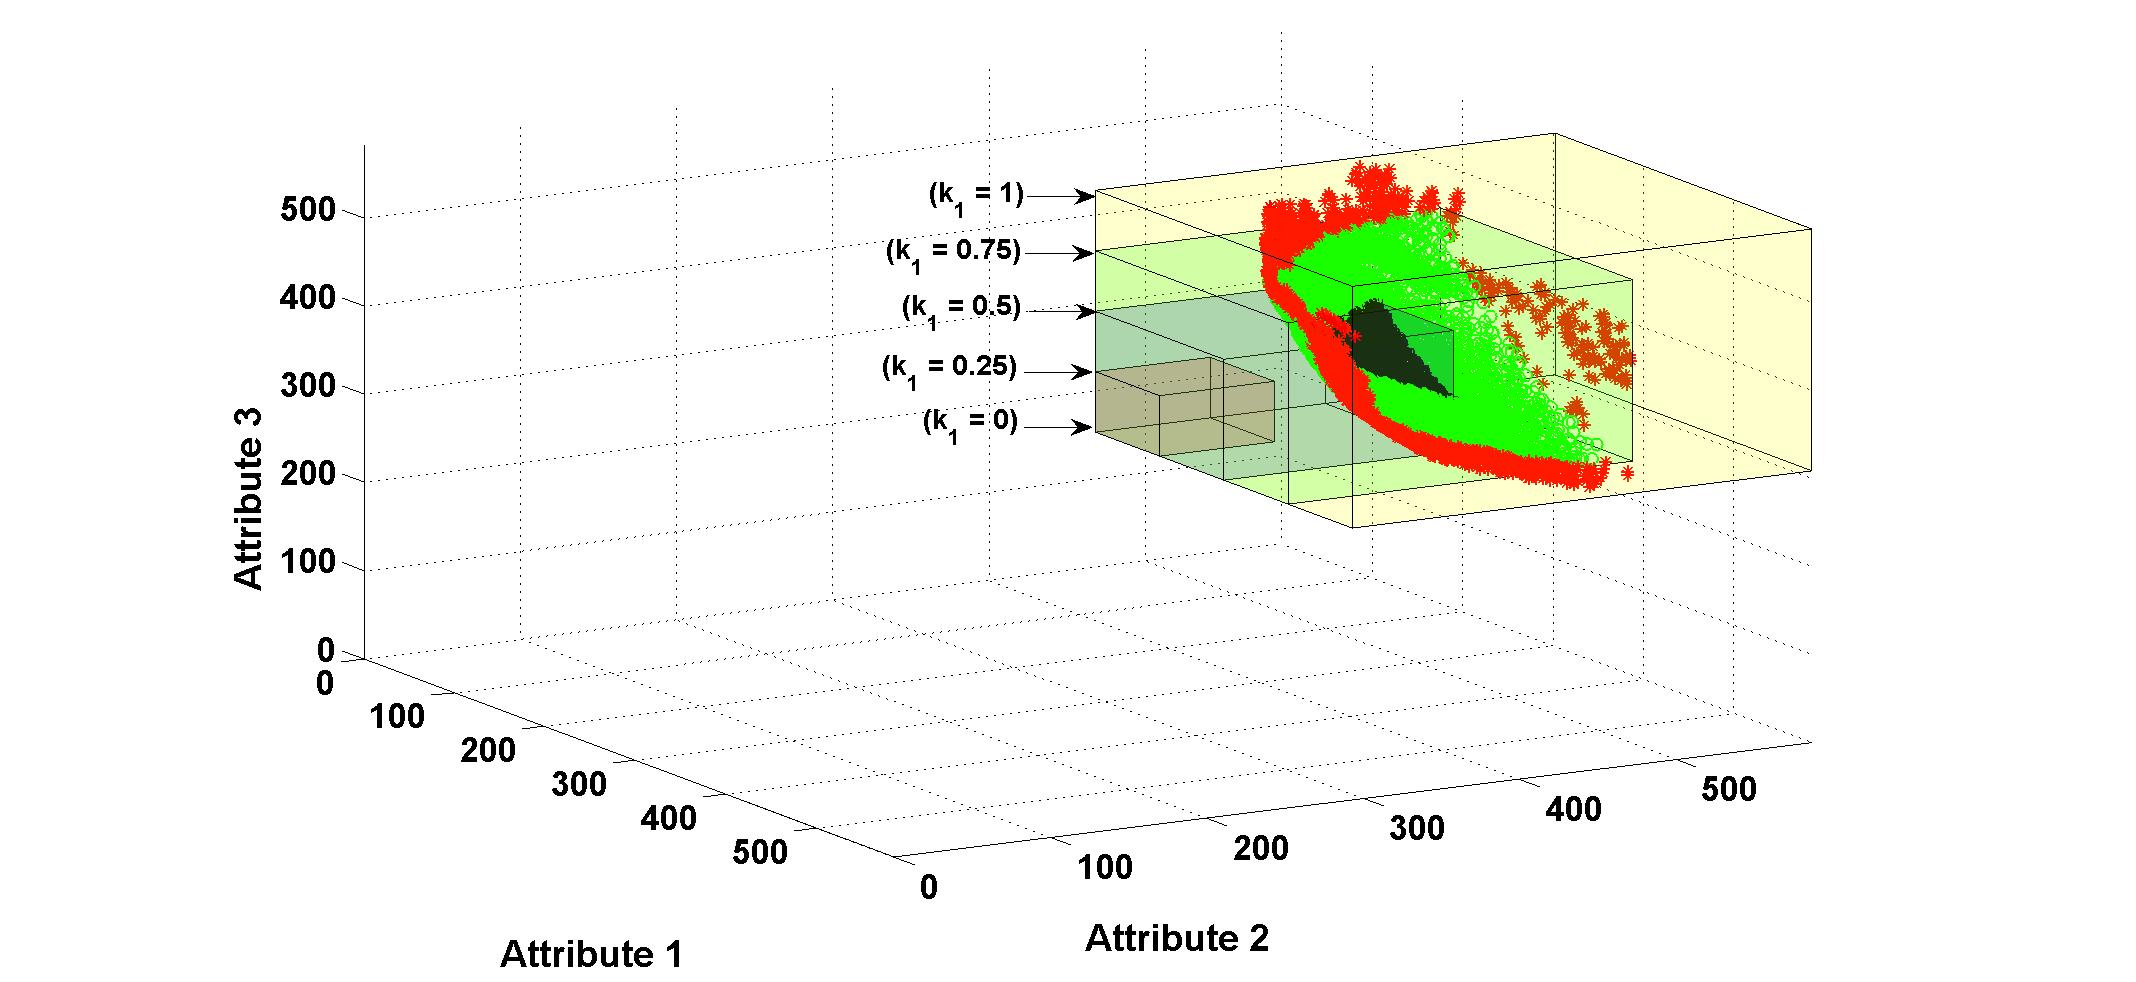
\includegraphics[width=1\textwidth]{Images/Chapter6/class1-3d-p45}
\caption{Three-dimensional Pareto frontier divided according to goal satisfiability for a sample problem with solution depth $d = 100$.}
\label{fig:6-1}
\end{figure}

Figures \ref{fig:6-2} and \ref{fig:6-3} display the average number of scanned labels and average runtimes of \lexgo and \namoa, respectively, both as a function of solution depth. In these graphics, we observe that \lexgolex \ (\ref{fig:6-3a}) achieves important reductions in time of almost one order of magnitude for $k_1=0.5$, two orders of magnitude for $k_1=0.25$, and up to four orders of magnitude for $k_1=0$. These are explained in large part by the reduction observed in the number of labels scanned, i.e. half the number of labels for $k_1=0.5$, around one order of magnitude less for $k_1=0.25$ and three orders of magnitude less for $k_1=0$. 

\begin{figure}%[!ht]
\centering
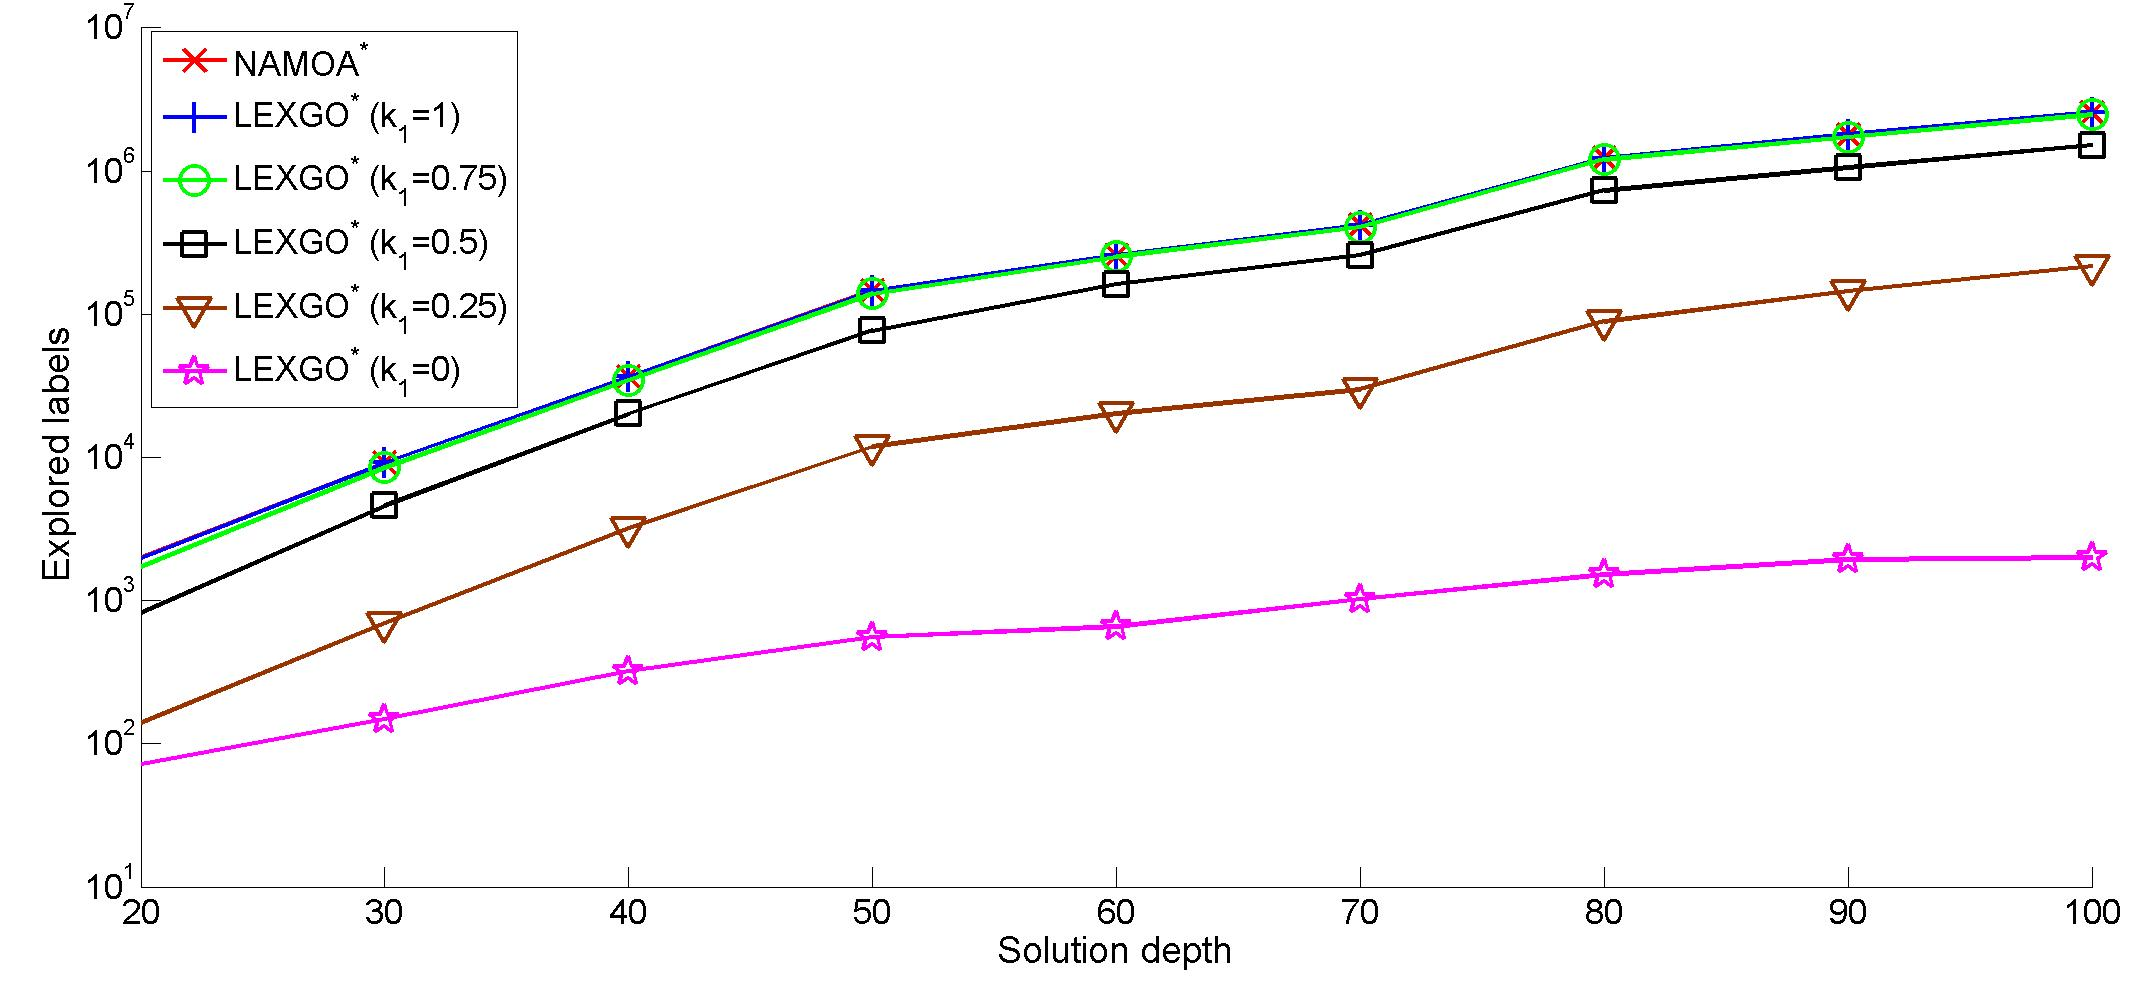
\includegraphics[width=1\textwidth]{Images/Chapter6/class1-labels-lex}
\caption{Class I experiments on grids, average number of scanned (explored) labels per solution depth for lexicographic selection order.}
\label{fig:6-2}
\end{figure}

Figure \ref{fig:6-3b} shows the average runtimes of \lexgolin \ and \namoalin. A small time overhead is also found for $k_1=0.75$ in the linear case, as well as poorer results when $k_1=0.5$. Notice that \namoalin \ is shown to be approximately two times faster than \namoalex. These results regarding the importance of the selection order are consistent with other recent studies \citep{Machuca2011, Iori2010}. However, \lexgolin \ is not always more efficient than \lexgolex. For $k_1= 1$ and $k_1= 0.75$ the linear aggregation order guides the search to find the solutions later than the lexicographic order and speeds up the runtime performance of algorithms that use the linear order whenever a big amount of solutions exist, due to a smaller number of filtering comparisons are needed. We further analyze in Section \ref{chapEmpiricalAnalysis:sec:resultsgridsnamoate} the impact of the number of pruning and filtering comparisons in runtime performance.

\begin{figure}
    \begin{center}
%
      \subfigure[Lexicographic selection order]{%
         \label{fig:6-3a}
        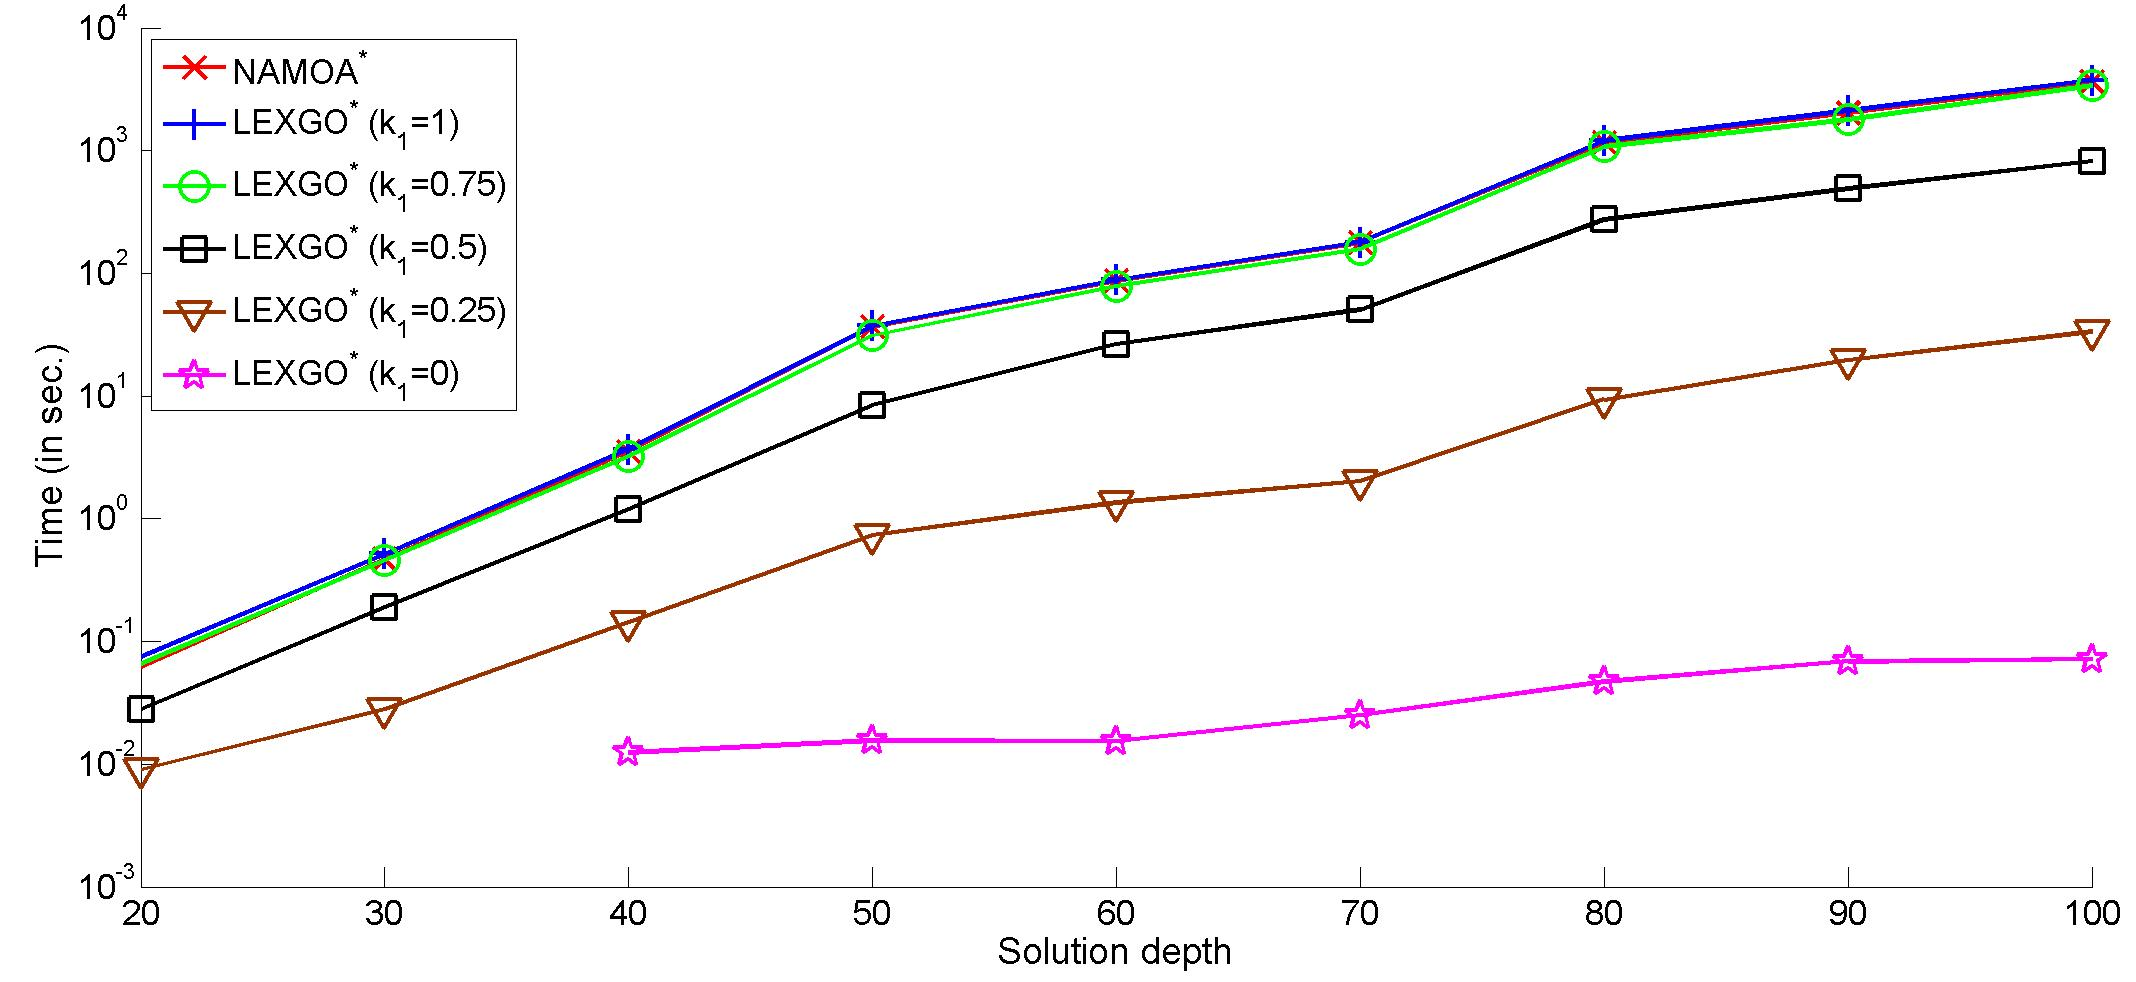
\includegraphics[width=0.95\textwidth]{Images/Chapter6/class1-exe-time-lex}
        }\\ %  ------- End of the first row ----------------------%
\vspace{0.025\textwidth}      
\subfigure[linear aggregation selection order]{%
         \label{fig:6-3b}
        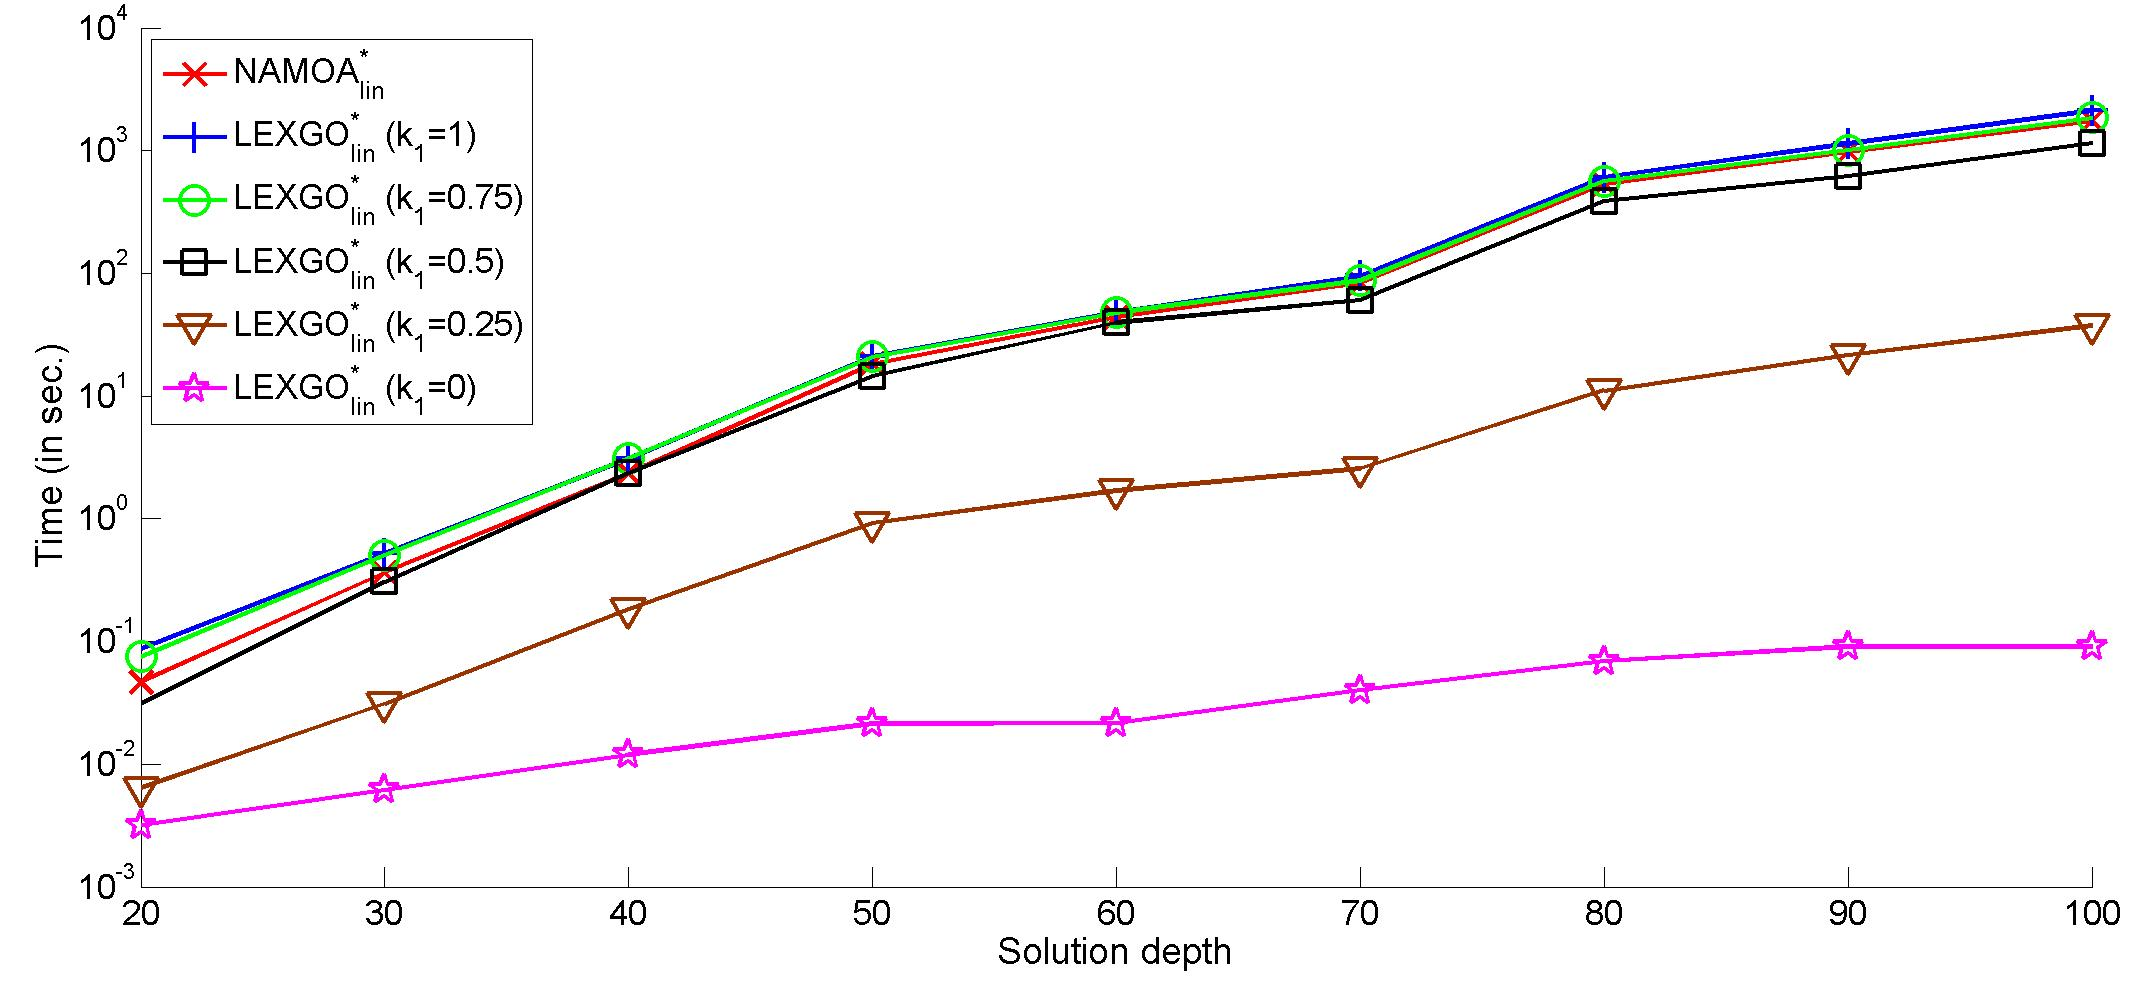
\includegraphics[width=0.95\textwidth]{Images/Chapter6/class1-exe-time-lin}
        }\\ %  ------- End of the first row ----------------------%
    \end{center}
    \vspace{-0.25in} 
    \caption{%
Class I experiments on grids, average runtime in seconds per solution depth for \namoa \ and \lexgo.  
    }%
    \label{fig:6-3}
\end{figure}

Table \ref{tab:6-2} summarizes the space and runtime performance of \lexgo \ relative to \namoa \ for $d = 100$ with the lexicographic and linear aggregation selection orders, respectively. The space performance is measured in scanned labels ($\sum G_{cl}$) and the runtime performance in seconds. 

A small time overhead can be observed for \lexgolex \ with $k_1= 1$ when compared with \namoalex. This time overhead is greater for \lexgolin, due to the comparison with the more efficient version of \namoa \ with the linear aggregation order. The time difference can be attributed to the extra calculations of deviation from targets needed by \lexgo \ for all labels, and the extra checks for pruning and filtering that do not provide any advantage in this situation.

No significant difference is found regarding the scanned labels by \namoalex \ and \namoalin, or the relative number to \lexgolex \ and \lexgolin. In fact, \namoa \ should expand the same labels regardless of the selection order policy. However, the lazy filtering technique introduces a slight variation which is found not to be significant in any case (see \cite{SandersMandow2013} for a more detailed explanation of the lazy filtering technique). 

\begin{table}
\caption{%
    Class I experiments on grids, summary of the relative space and runtime performance of \lexgo \ over \namoa \ for $d = 100$ experiments.
     }%
\vspace{0.05\textwidth}
\begin{center}
        \subtable[Relative space performance of \lexgolex \ over \namoalex]{%
\label{tab:6-2a}
\begin{tabular}{rrrrrrr}
\hline \noalign{\smallskip}
& \multicolumn{5}{c}{\lexgolex} \\
\noalign{\smallskip} \cline{2-6} \noalign{\smallskip}
\namoalex & 1 & 0.75 & 0.5 & 0.25 & 0 & \multicolumn{1}{c}{$k_1$} \\
\noalign{\smallskip} 
$\sum G_{cl}$ & \% & \% & \% & \% & \% \\
\cline{1-6}  \noalign{\smallskip} 
2,550,354 & 99.9 & 96.9 & 59.2 & 8.5 & 0.08 \\
\hline
\end{tabular}
        }%
\vspace{0.05\textwidth} % To get a little bit of space between the figures
        \subtable[Relative space performance of \lexgolin \ over \namoalin]{%
\label{tab:6-2b}
\begin{tabular}{rrrrrrr}
\hline \noalign{\smallskip}
& \multicolumn{5}{c}{\lexgolin} \\
\noalign{\smallskip} \cline{2-6} \noalign{\smallskip}
\namoalin & 1 & 0.75 & 0.5 & 0.25 & 0 & \multicolumn{1}{c}{$k_1$} \\
\noalign{\smallskip} 
$\sum G_{cl}$ & \% & \% & \% & \% & \% \\
\cline{1-6}  \noalign{\smallskip}  
2,598,427 & 99.9 & 97.2 & 59.1 & 8.3 & 0.08 \\
\hline
\end{tabular}
        }\\ %  ------- End of the first row ----------------------%
\vspace{0.05\textwidth}
        \subtable[Relative runtime performance of \lexgolex \ over \namoalex]{%
\label{tab:6-2c}
\begin{tabular}{rrrrrrr}
\hline \noalign{\smallskip}
& \multicolumn{5}{c}{\lexgolex} \\
\noalign{\smallskip} \cline{2-6} \noalign{\smallskip}
\namoalex & 1 & 0.75 & 0.5 & 0.25 & 0 & \multicolumn{1}{c}{$k_1$} \\
\noalign{\smallskip} 
Runtime (s) & \% & \% & \% & \% & \% \\
\cline{1-6}  \noalign{\smallskip} 
3,662.9 & 102.7 & 92.3 & 22.3 & 0.9 & 0.001 \\
\hline
\end{tabular}
        }%  %  ------- End of the second row ----------------------%
\vspace{0.05\textwidth}
        \subtable[Relative runtime performance of \lexgolin \ over \namoalin]{%
\label{tab:6-2d}
\begin{tabular}{rrrrrrr}
\hline \noalign{\smallskip}
& \multicolumn{5}{c}{\lexgolin} \\
\noalign{\smallskip} \cline{2-6} \noalign{\smallskip}
\namoalin & 1 & 0.75 & 0.5 & 0.25 & 0 & \multicolumn{1}{c}{$k_1$} \\
\noalign{\smallskip} 
Runtime (s) & \% & \% & \% & \% & \% \\
\cline{1-6}  \noalign{\smallskip} 
1,754.4 & 120.5 & 105.3 & 65.2 & 2.1 & 0.005 \\
\hline
\end{tabular}
        }%  %  ------- End of the third row ----------------------%
\end{center}
\label{tab:6-2}
\end{table}

%-------------------------------------------------------------------
\subsection{Analysis on class II experiments}
\label{chapEmpiricalAnalysis:subsec:analysisgridslexgoc2}
%-------------------------------------------------------------------

Target values in the second class of experiments were defined using $k_1 = \{0.75 , 0.5\}$, where $k_2$ is defined as in Equation \ref{eq:targets2}. This allows us to analyze the case where targets for one goal are proportionally stricter, and the extreme case where some goals are satisfied and some not. 

Tables \ref{tab:6-3} and \ref{tab:6-4} show percentages of Pareto goal-optimal solution costs and scanned labels of all values of $k_2$ in \lexgo \ relative to \namoa. Figure \ref{fig:6-4} displays the average number of scanned labels as a function of solution depth for $k_1= 0.75$ and $k_1= 0.5$.

\begin{table}
\caption{Class II experiments on grids, \lexgo \ average percentage of goal-optimal solution costs relative to $C^*$. An asterisk ($^*$) indicates some of the five instances could not satisfy all goals, and two asterisks ($^{**}$) that none of the five instances could satisfy all goals.}
\centering
\begin{tabular}{rrrrrrrrrrr}
\hline \noalign{\smallskip}
 & & \multicolumn{8}{c}{\lexgo} & \\
\noalign{\smallskip} \cline{3-10}
\multicolumn{2}{c}{} & \multicolumn{4}{c|}{0.75} & \multicolumn{4}{c}{0.5} & \multicolumn{1}{c}{$k_1$}\\
 & \namoa & 0.75 & 0.5625 & 0.375 & \multicolumn{1}{c|}{0.1875} & 0.5 & 0.375 & 0.25 & 0.125 & \multicolumn{1}{c}{$k_2$}\\
\noalign{\smallskip} 
$d$ & Avg. $|C^*|$ & \% & \% & \% & \% & \% & \% & \% & \% & \\
\cline{1-10} \noalign{\smallskip} 
20 & 122 & 74.3 & 59.1 & 35.2 & 10.6 & 20.5 & 11.5 & 3.3 & $^*$0.82 \\ 
30 & 302 & 77.6 & 63.4 & 38.5 & 15.5 & 22.2 & 12.3 & 5.6 & $^*$1.00 \\
40 & 694 & 78.7 & 59.3 & 34.0 & 12.2 & 20.8 & 10.5 & 3.3 & $^{**}$0.14 \\
50 & 1,599 & 78.2 & 57.2 & 33.6 & 12.3 & 16.8 & 8.4 & 2.6 & $^*$0.06 \\
60 & 2,007 & 83.0 & 62.6 & 35.9 & 12.6 & 24.6 & 13.1 & 3.8 & $^*$0.25 \\ 
70 & 2,561 & 82.4 & 66.0 & 41.9 & 14.6 & 24.6 & 13.6 & 4.2 & $^*$0.12 \\ 
80 & 5,423 & 82.3 & 64.9 & 36.1 & 11.6 & 20.3 & 9.1 & 1.7 & $^{**}$0.02 \\ 
90 & 5,912 & 77.7 & 63.6 & 38.2 & 10.7 & 21.0 & 10.5 & 2.1 & $^{**}$0.02 \\ 
100 & 8,307 & 77.9 & 60.5 & 35.7 & 10.6 & 17.0 & 8.1 & 1.1 & $^{**}$0.01 
\\ 
\hline
\end{tabular}
\label{tab:6-3}
\end{table} 

\begin{table}
\caption{Class II experiments on grids, \lexgolex \ average percentage of scanned labels ($\sum G_{cl}$) compared to \namoalex.}
\centering
\begin{tabular}{rrrrrrrrrrr}
\hline \noalign{\smallskip}
 & & \multicolumn{8}{c}{\lexgolex} & \\
\noalign{\smallskip} \cline{3-10}
\multicolumn{2}{c}{} & \multicolumn{4}{c|}{0.75} & \multicolumn{4}{c}{0.5} & \multicolumn{1}{c}{$k_1$}\\
 & \namoalex & 0.75 & 0.5625 & 0.375 & \multicolumn{1}{c|}{0.1875} & 0.5 & 0.375 & 0.25 & 0.125 & \multicolumn{1}{c}{$k_2$}\\
\noalign{\smallskip} 
$d$ & $\sum G_{cl}$  & \% & \% & \% & \% & \% & \% & \% & \% & \\
\cline{1-10} \noalign{\smallskip} 
20 & 1,985 & 86.2 & 75.1 & 50.9 & 19.0 & 41.4 & 28.9 & 17.5 & 8.9 \\ 
30 & 9,164 & 92.4 & 83.1 & 55.5 & 20.3 & 50.3 & 34.8 & 18.9 & 11.0 \\
40 & 36,557 & 94.5 & 83.2 & 55.6 & 19.1 & 55.1 & 38.4 & 19.9 & 9.5 \\
50 & 145,823 & 95.5 & 83.4 & 54.7 & 18.3 & 52.7 & 36.4 & 18.2 & 7.5 \\
60 & 257,935 & 97.5 & 88.9 & 60.9 & 19.8 & 62.9 & 45.9 & 23.1 & 7.8 \\ 
70 & 420,056 & 96.6 & 88.9 & 63.5 & 21.2 & 61.5 & 45.7 & 23.5 & 7.2 \\ 
80 & 1,231,565 & 97.3 & 89.1 & 60.4 & 18.8 & 59.2 & 42.0 & 20.0 & 8.6 \\ 
90 & 1,789,607 & 96.7 & 88.8 & 62.9 & 20.0 & 59.1 & 43.1 & 21.6 & 10.3 \\ 
100 & 2,550,354 & 97.0 & 89.3 & 61.1 & 17.5 & 59.3 & 42.2 & 19.8 & 11.8 \\ 
\hline
\end{tabular}
\label{tab:6-4}
\end{table} 

\begin{figure}
    \begin{center}
%
      \subfigure[$k_1 = 0.75$]{%
         \label{fig:6-4a}
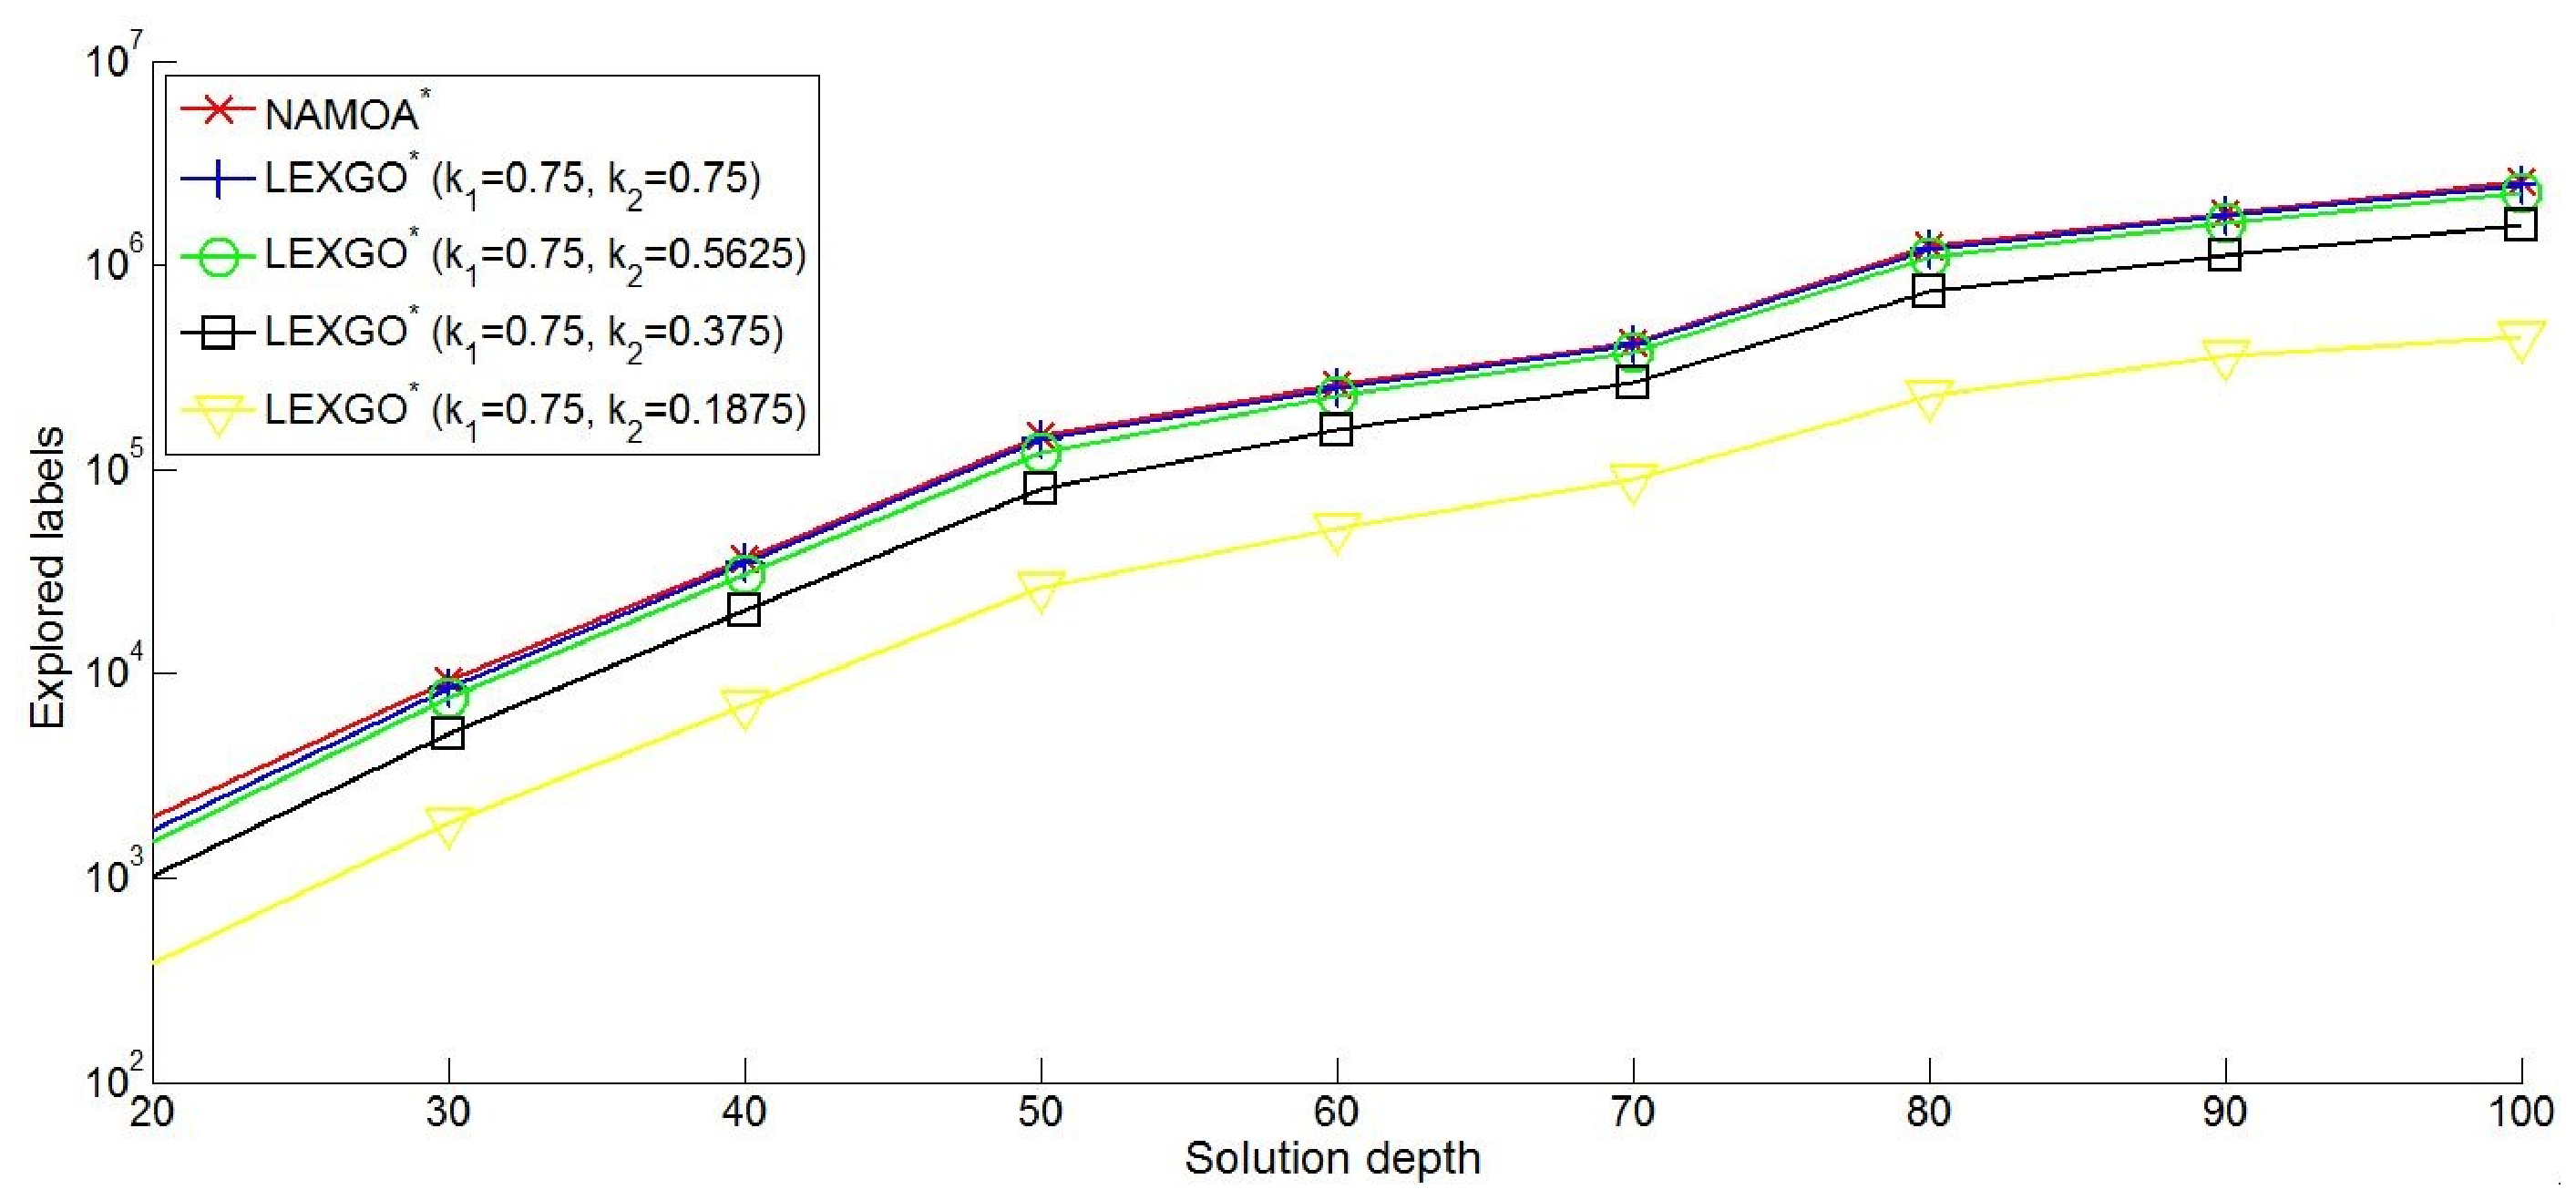
\includegraphics[width=0.95\textwidth]{Images/Chapter6/class2-labels075-lex}
        }\\ %  ------- End of the first row ----------------------%
\vspace{0.025\textwidth}      
		\subfigure[$k_1 = 0.5$]{%
         \label{fig:6-4b}  
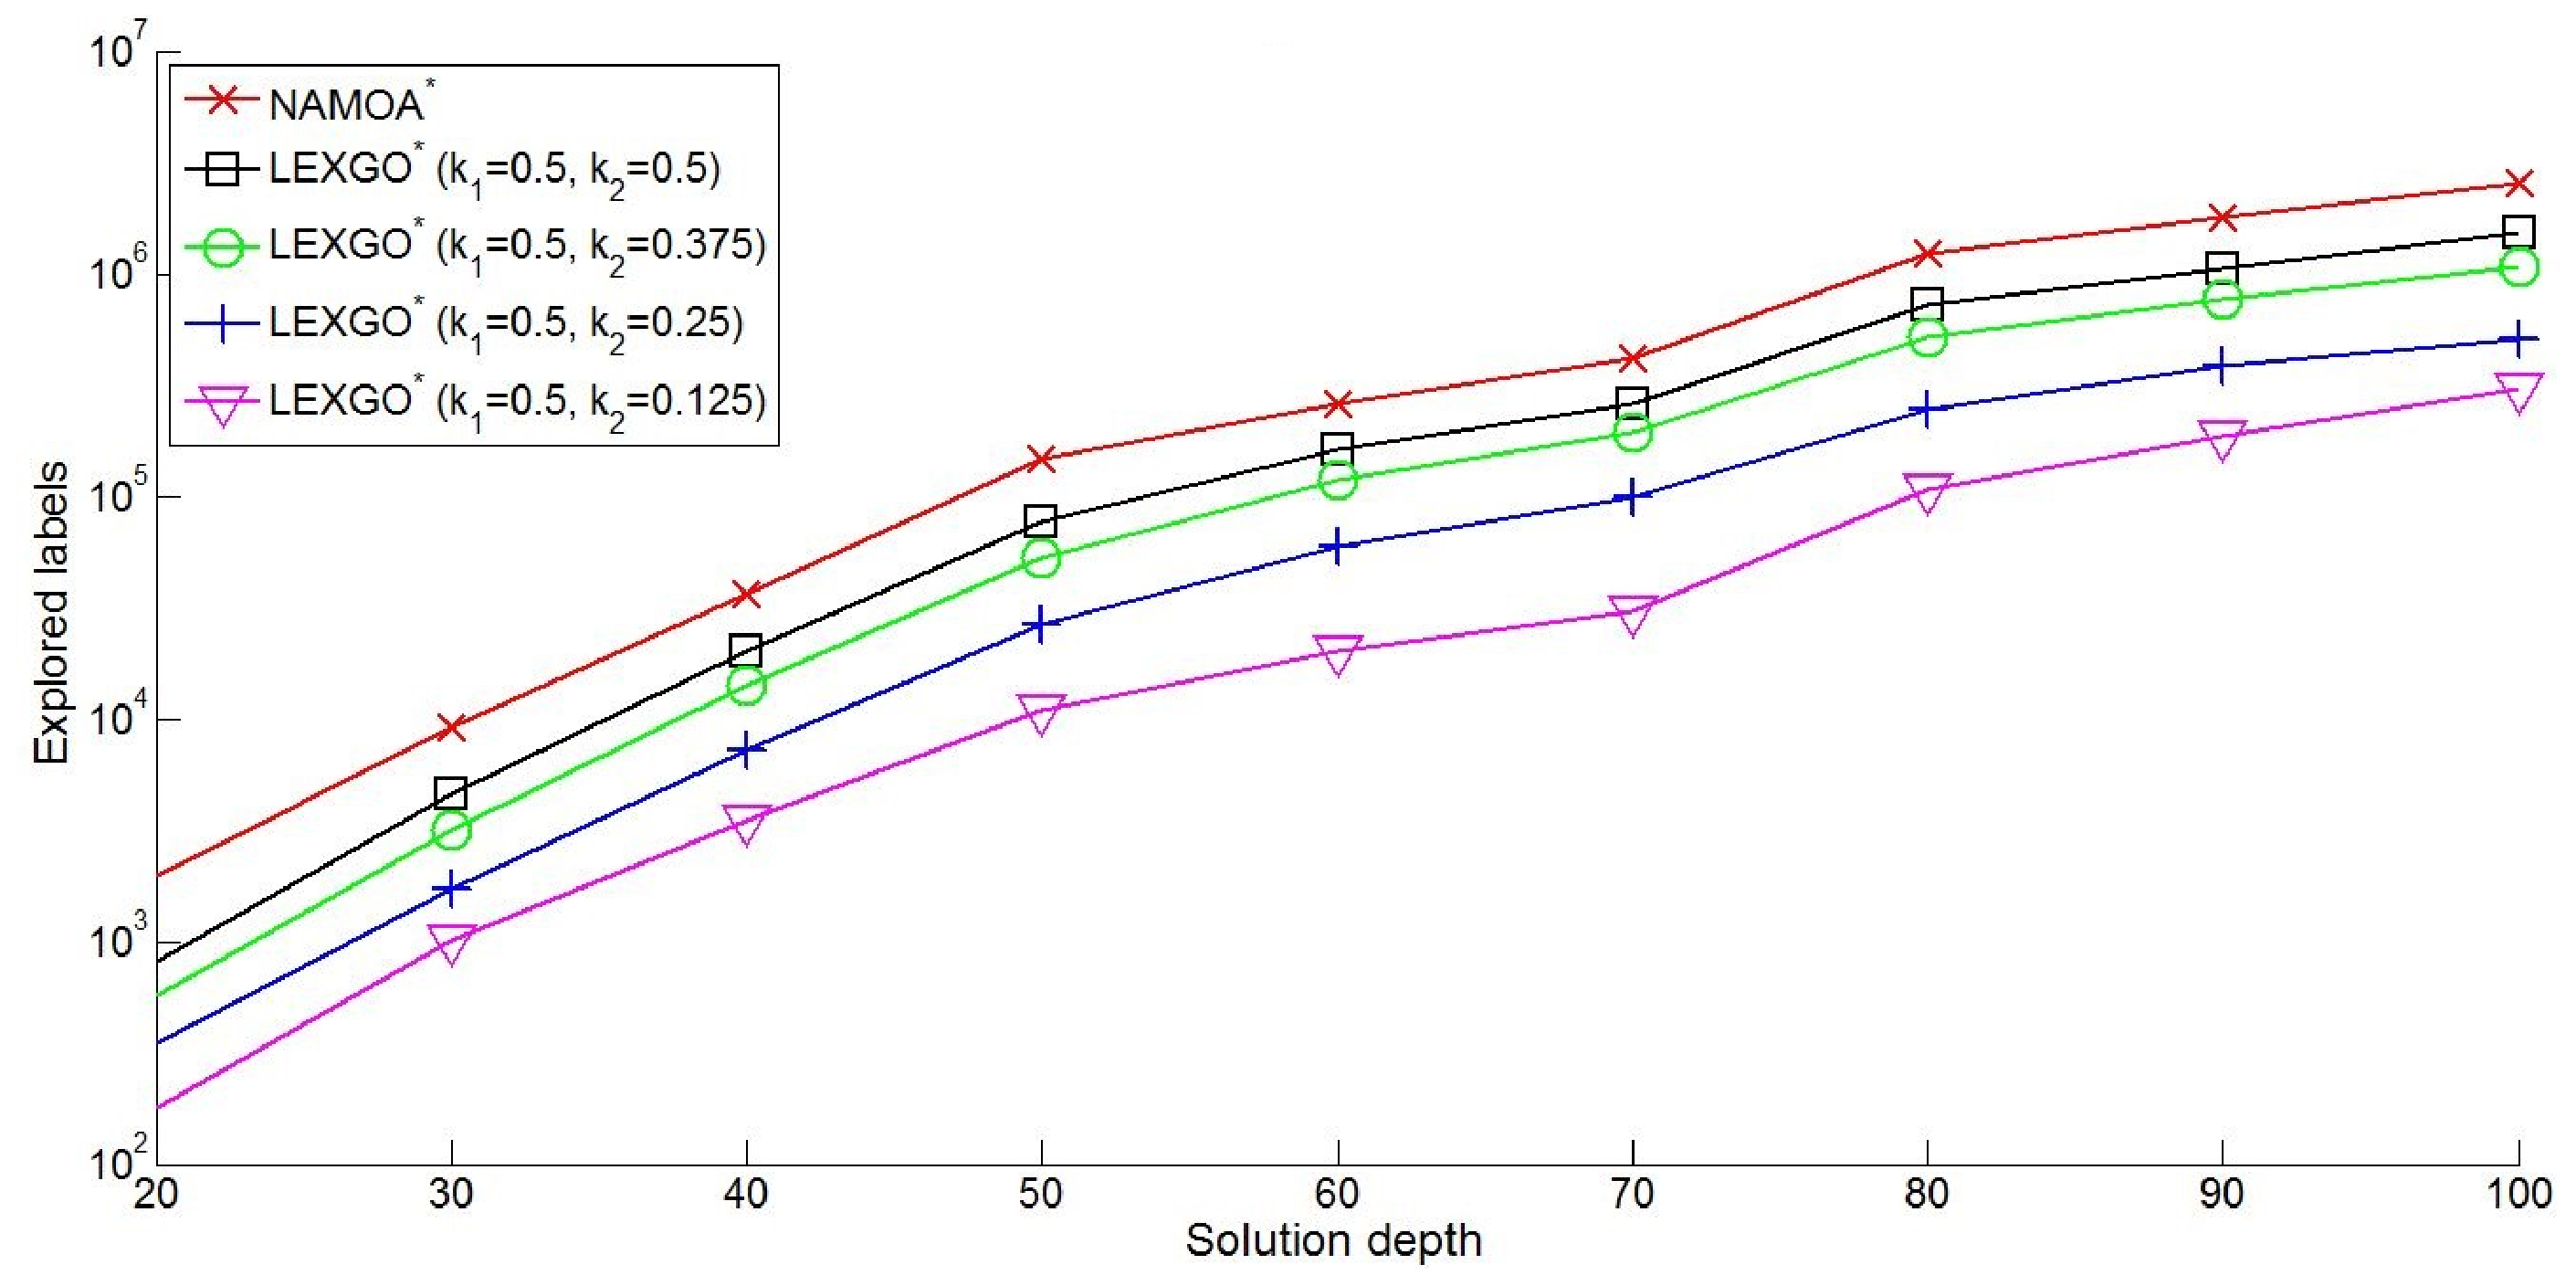
\includegraphics[width=0.95\textwidth]{Images/Chapter6/class2-labels05-lex}
        }\\ %  ------- End of the first row ----------------------%
    \end{center}
    \vspace{-0.25in} 
    \caption{%
Class II experiments on grids, average scanned labels per solution depth for \namoa \ and \lexgo \ with lexicographic selection order.  
    }%
    \label{fig:6-4}
\end{figure}

Table \ref{tab:6-5} displays the relative percentage of \lexgo \ runtimes to \namoa \ employing lexicographic and linear selection orders. In a graphical manner, Figures \ref{fig:6-5} and \ref{fig:6-6} show, respectively, average runtimes for  $k_1 = 0.75$ and $k_1 = 0.5$ with lexicographic and linear selection orders.

\begin{table}
\caption{%
Class II experiments on grids, \lexgo \ runtimes (in seconds) percentage relative to \namoa.
     }%
\begin{center}
        \subtable[Lexicographic selection order]{%
\label{tab:6-5a}
\scalebox{.95}{
\begin{tabular}{rrrrrrrrrrr}
\hline \noalign{\smallskip}
 & & \multicolumn{8}{c}{\lexgolex} & \\
\noalign{\smallskip} \cline{3-10}
\multicolumn{2}{c}{} & \multicolumn{4}{c|}{0.75} & \multicolumn{4}{c}{0.5} & \multicolumn{1}{c}{$k_1$}\\
 & \namoalex & 0.75 & 0.5625 & 0.375 & \multicolumn{1}{c|}{0.1875} & 0.5 & 0.375 & 0.25 & 0.125 & \multicolumn{1}{c}{$k_2$}\\
\noalign{\smallskip} 
$d$ & Runtime (s) & \% & \% & \% & \% & \% & \% & \% & \% & \\
\cline{1-10} \noalign{\smallskip} 
20 & 0.06 & 100.0 & 66.6 & 50.0 & 16.6 & 33.3 & 16.6 & 1.6 & 1.6 \\ 
30 & 0.4 & 112.5 & 95.0 & 55.0 & 17.5 & 47.5 & 30.0 & 17.5 & 12.5 \\ 
40 & 3.5 & 91.4 & 68.5 & 34.2 & 8.5 & 34.2 & 20.0 & 8.5 & 5.7 \\ 
50 & 36.8 & 84.7 & 60.0 & 25.8 & 4.6 & 22.8 & 12.5 & 4.8 & 1.9 \\ 
60 & 86.9 & 90.6 & 67.4 & 29.4 & 4.4 & 30.4 & 16.6 & 5.8 & 1.8 \\  
70 & 178.5 & 88.4 & 67.5 & 31.2 & 4.9 & 28.1 & 15.1 & 5.3 & 1.4 \\
80 & 1,164.1 & 92.2 & 69.5 & 27.8 & 3.4 & 23.5 & 11.6 & 3.4 & 1.4 \\ 
90 & 2,030.0 & 87.7 & 69.0 & 31.4 & 3.7 & 24.1 & 12.6 & 3.9 & 1.9 \\ 
100 & 3,662.9 & 92.3 & 66.7 & 27.6 & 2.9 & 22.3 & 11.1 & 3.3 & 2.1 \\ 
\hline
\end{tabular}
}
        }%
\vspace{0.05\textwidth} % To get a little bit of space between the figures
        \subtable[linear aggregation selection order]{%
\label{tab:6-5b}
\scalebox{.95}{
\begin{tabular}{rrrrrrrrrrr}
\hline \noalign{\smallskip}
 & & \multicolumn{8}{c}{\lexgolin} & \\
\noalign{\smallskip} \cline{3-10}
\multicolumn{2}{c}{} & \multicolumn{4}{c|}{0.75} & \multicolumn{4}{c}{0.5} & \multicolumn{1}{c}{$k_1$}\\
 & \namoalin & 0.75 & 0.5625 & 0.375 & \multicolumn{1}{c|}{0.1875} & 0.5 & 0.375 & 0.25 & 0.125 & \multicolumn{1}{c}{$k_2$}\\
\noalign{\smallskip} 
$d$ & Runtime (s) & \% & \% & \% & \% & \% & \% & \% & \% & \\
\cline{1-10} \noalign{\smallskip} 
20 & 0.04 & 160.3 & 146.6 & 100.4 & 40.2 & 66.2 & 46.6 & 32.9 & 19.7 \\ 
30 & 0.3 & 138.4 & 149.5 & 99.9 & 30.8 & 83.8 & 58.1 & 28.2 & 16.3 \\ 
40 & 2.3 & 131.3 & 174.6 & 104.2 & 25.4 & 99.7 & 62.7 & 26.3 & 11.5 \\ 
50 & 18.3 & 113.6 & 144.0 & 92.5 & 17.6 & 79.2 & 50.4 & 18.1 & 5.3 \\ 
60 & 43.8 & 108.8 & 138.6 & 95.8 & 16.1 & 90.2 & 61.9 & 22.6 & 4.8 \\  
70 & 83.3 & 104.4 & 117.4 & 101.3 & 19.5 & 72.6 & 56.9 & 21.2 & 4.2 \\
80 & 533.8 & 105.5 & 138.3 & 96.4 & 13.8 & 72.6 & 49.6 & 14.6 & 4.0 \\ 
90 & 981.3 & 102.6 & 121.4 & 92.4 & 12.8 & 63.3 & 48.2 & 15.5 & 4.8 \\ 
100 & 1,754.4 & 105.3 & 130.2 & 98.0 & 11.1 & 65.3 & 46.1 & 13.1 & 5.3 \\ 
\hline
\end{tabular}
}
        }\\ %  ------- End of the first row ----------------------%
\end{center}
\label{tab:6-5}
\end{table}

\begin{figure}
    \begin{center}
%
      \subfigure[$k_1 = 0.75$]{%
         \label{fig:6-5a}
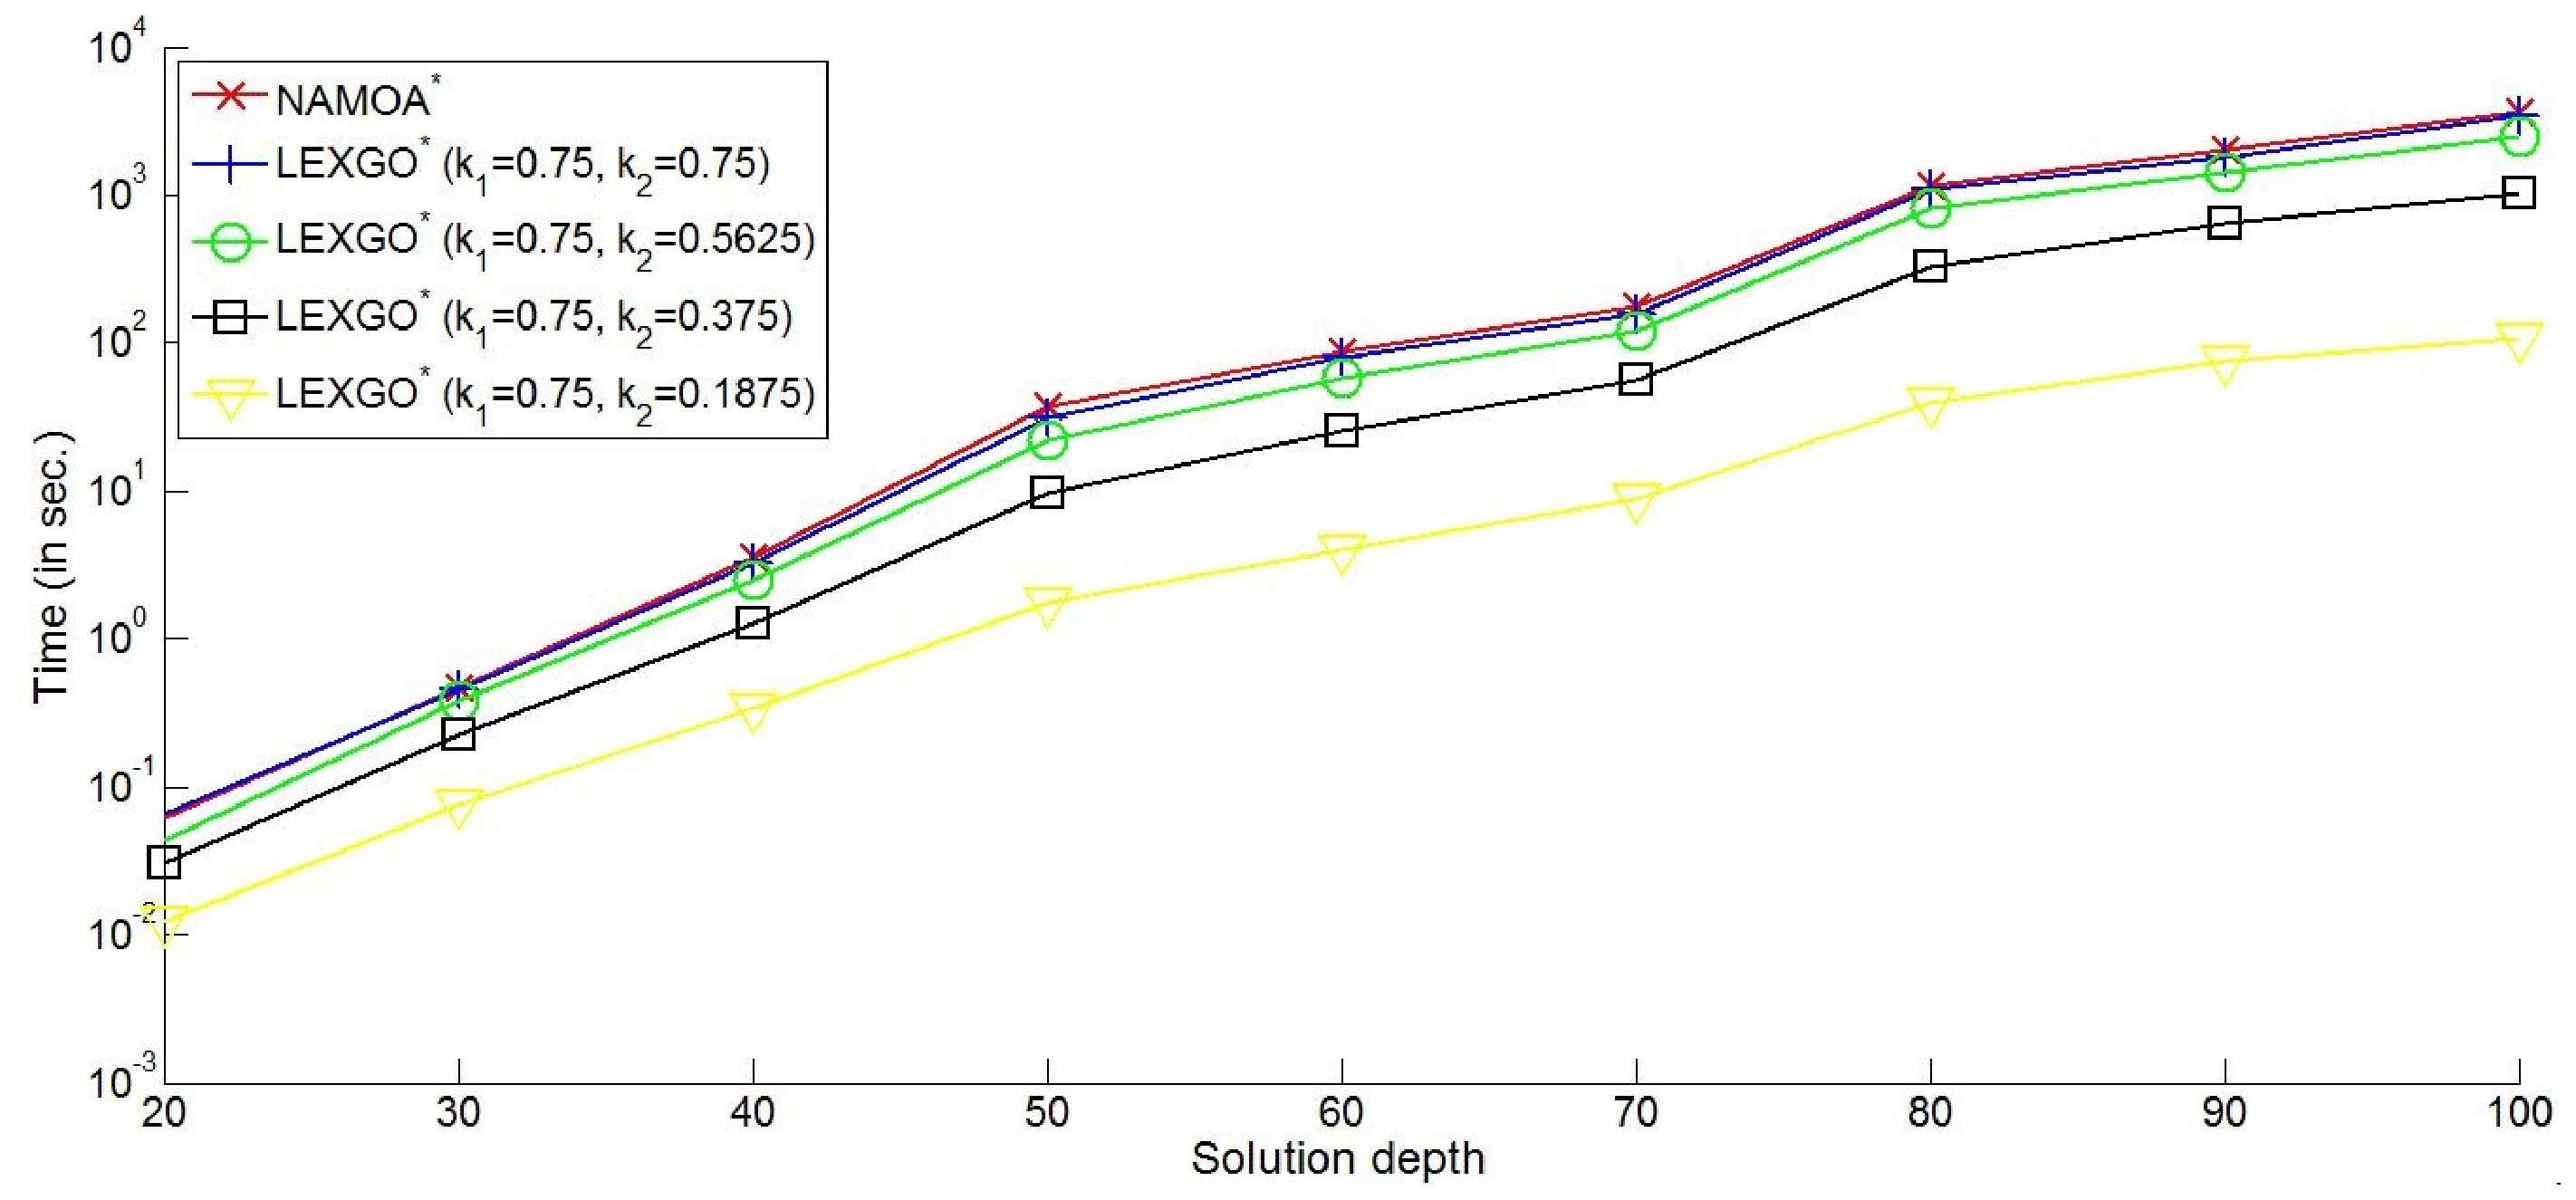
\includegraphics[width=0.95\textwidth]{Images/Chapter6/class2-exe075-lex}
        }\\ %  ------- End of the first row ----------------------%
\vspace{0.025\textwidth}      
		\subfigure[$k_1 = 0.5$]{%
         \label{fig:6-5b}  
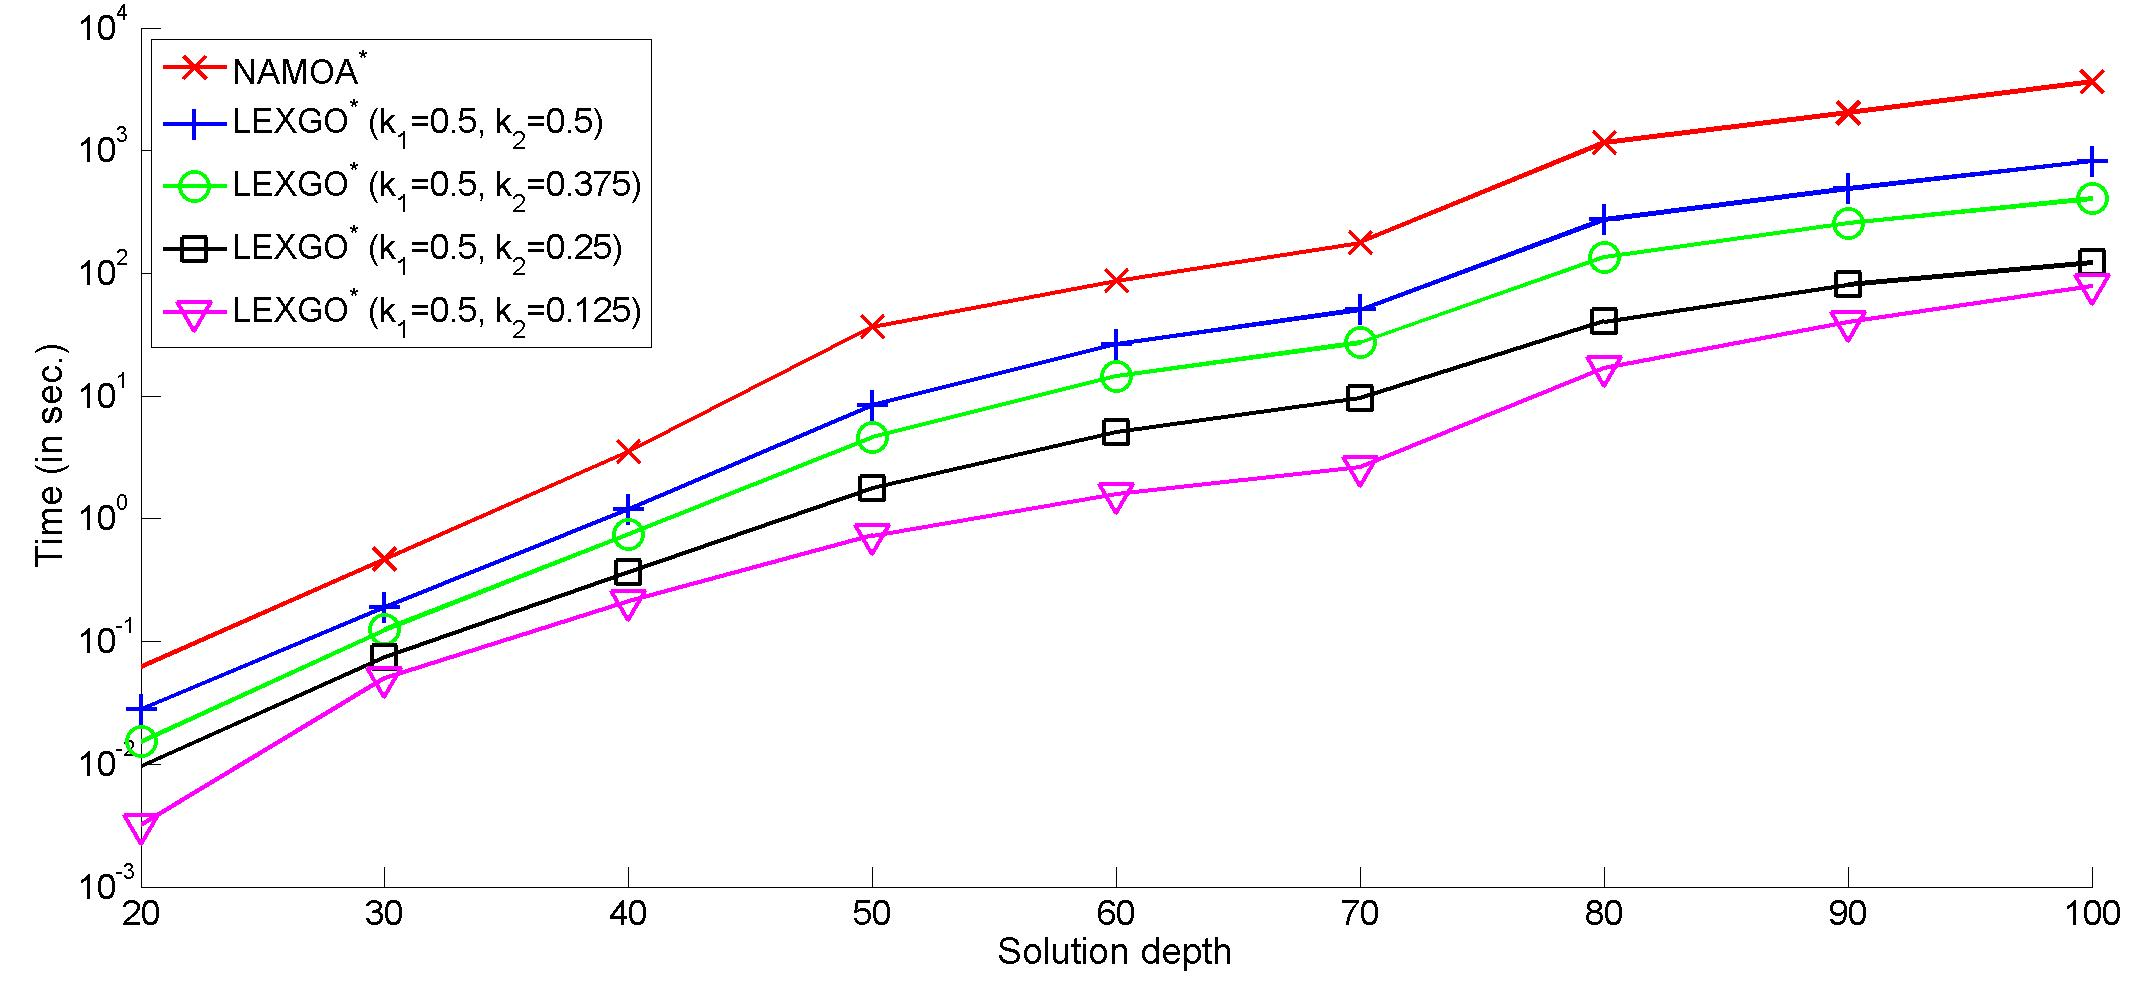
\includegraphics[width=0.95\textwidth]{Images/Chapter6/class2-exe05-lex}
        }\\ %  ------- End of the first row ----------------------%
    \end{center}
    \vspace{-0.25in} 
    \caption{%
Class II experiments on grids, average runtime (in seconds) per solution depth for \lexgo \ and \namoa \ with lexicographic selection order. 
    }%
    \label{fig:6-5}
\end{figure}

\begin{figure}
    \begin{center}
%
      \subfigure[$k_1 = 0.75$]{%
         \label{fig:6-6a}
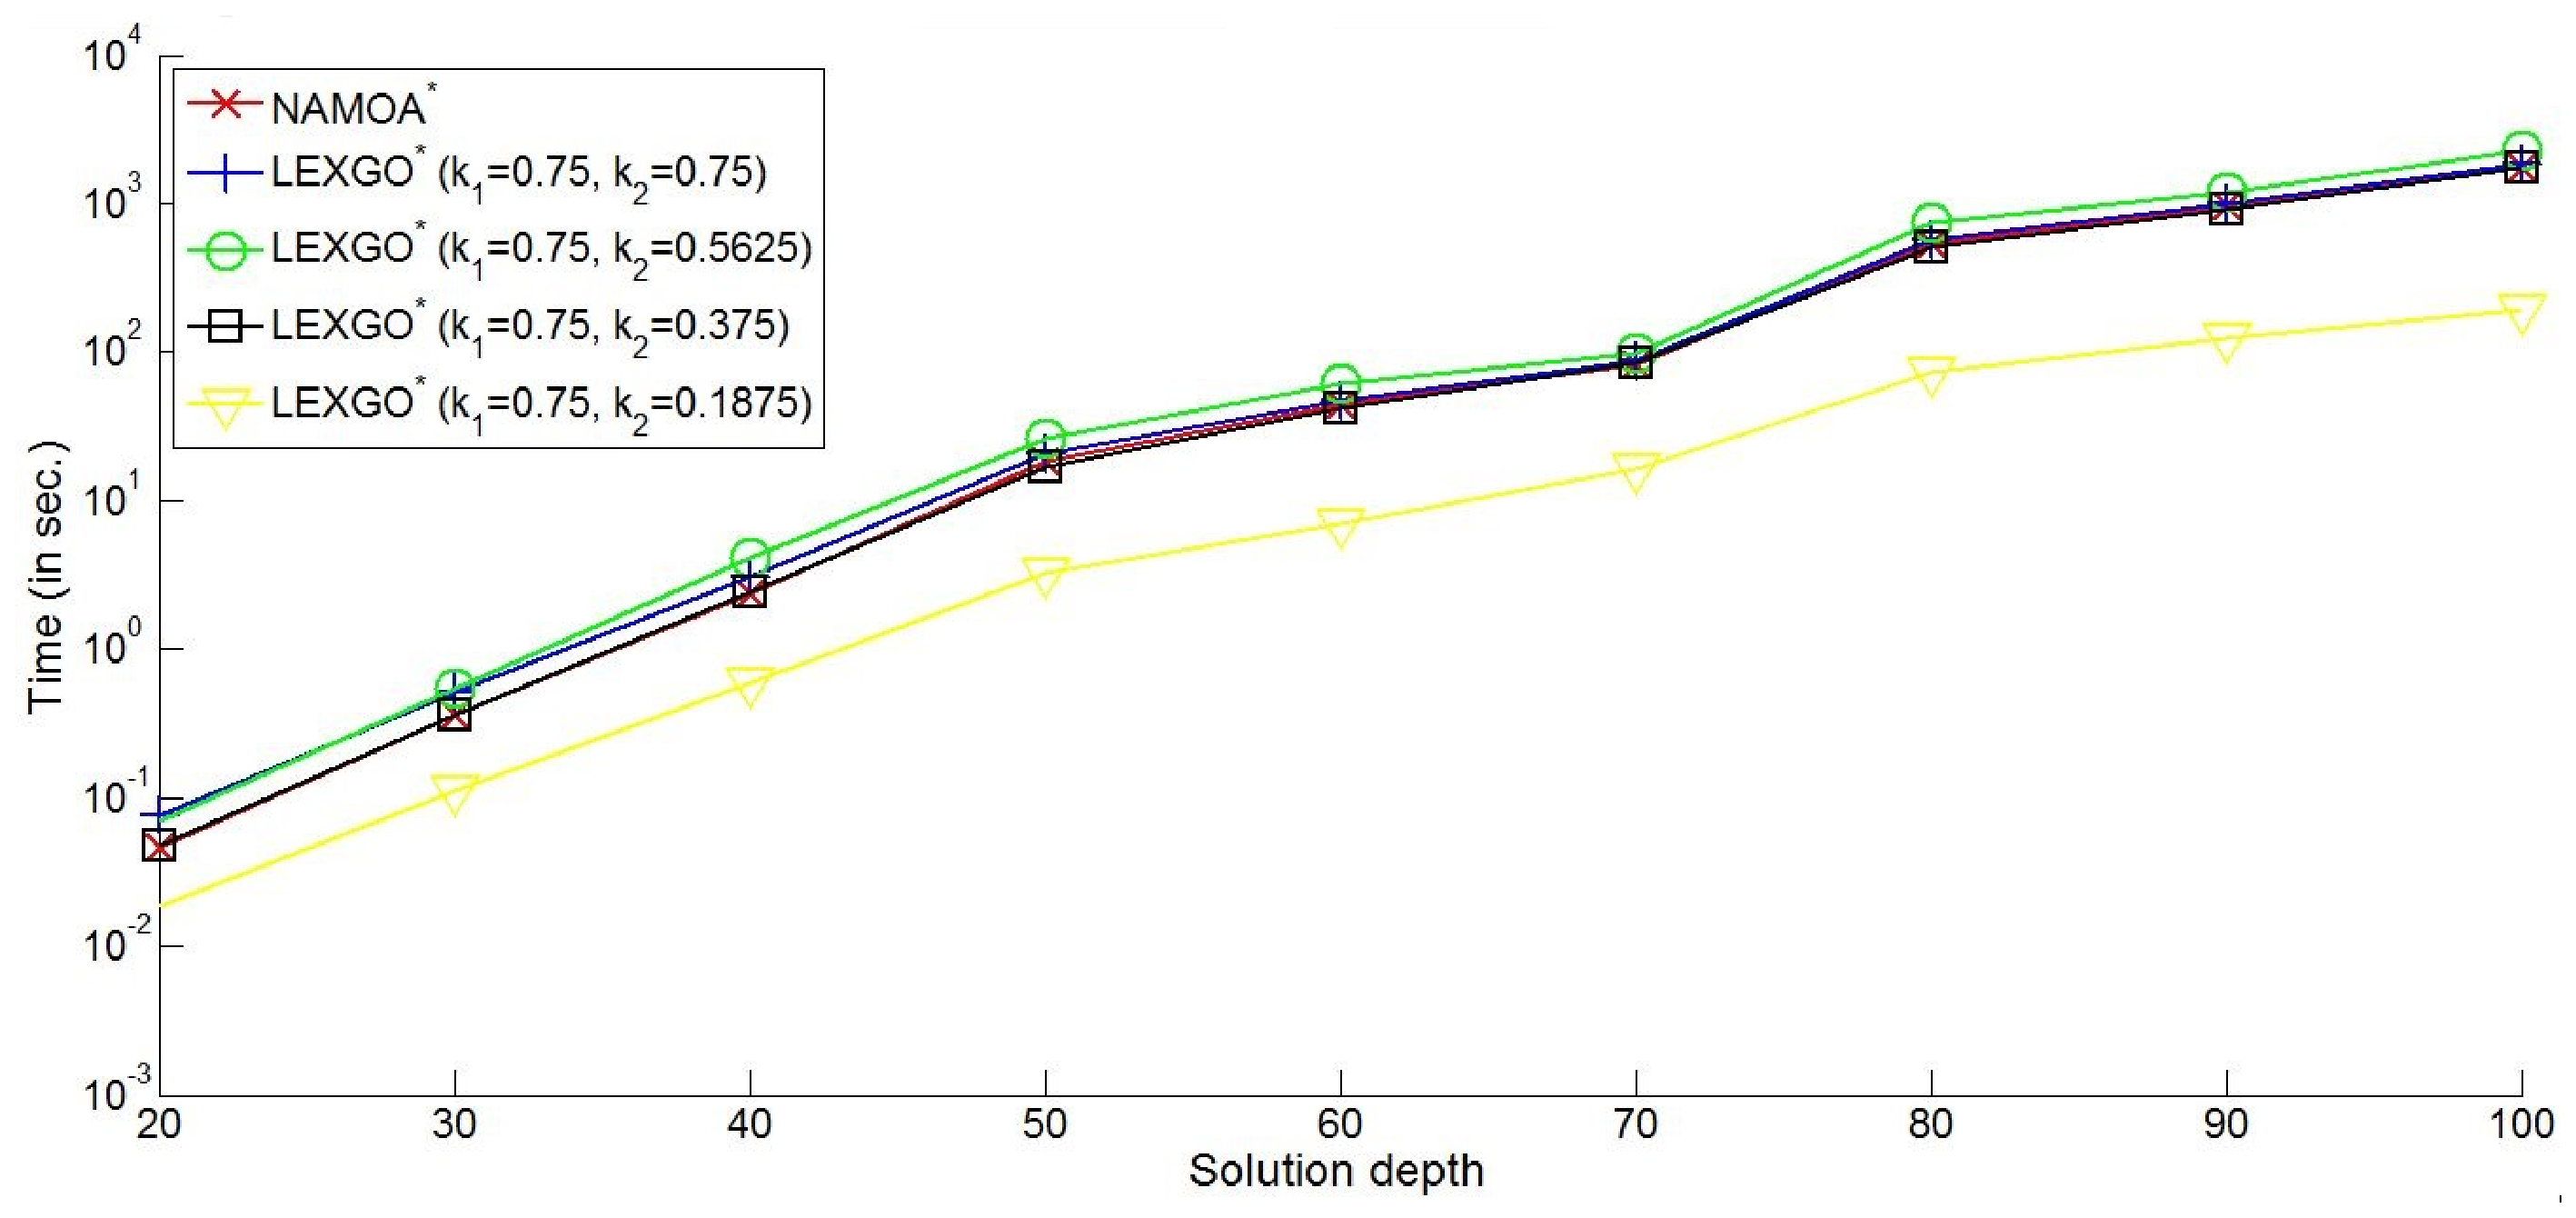
\includegraphics[width=0.95\textwidth]{Images/Chapter6/class2-exe075-lin}
        }\\ %  ------- End of the first row ----------------------%
\vspace{0.025\textwidth}      
		\subfigure[$k_1 = 0.5$]{%
         \label{fig:6-6b}  
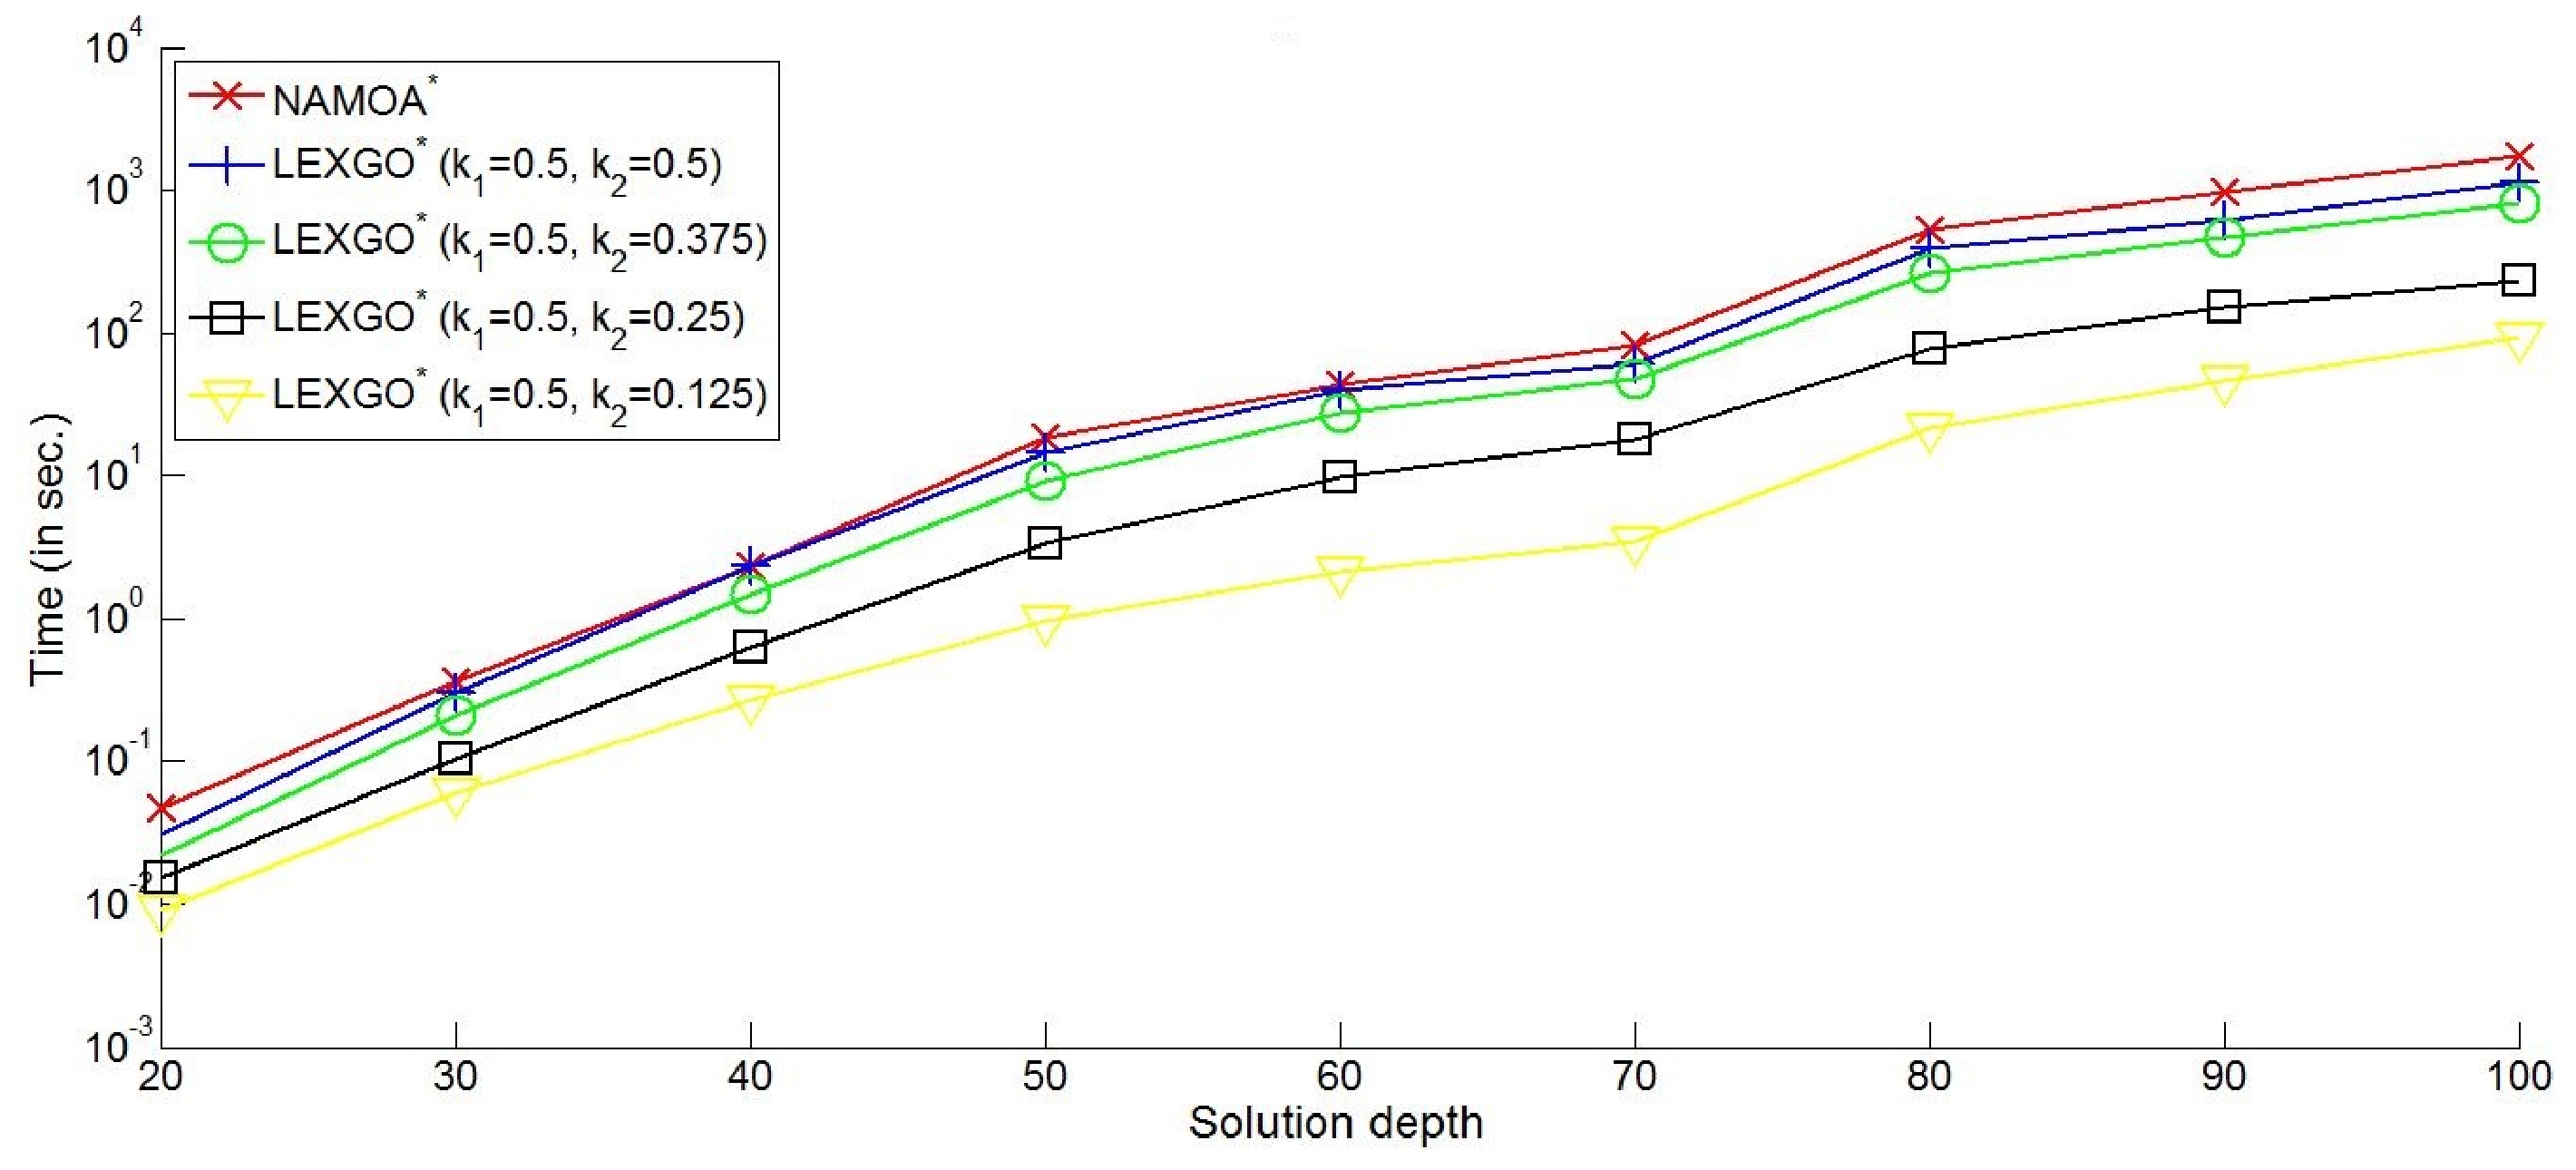
\includegraphics[width=0.95\textwidth]{Images/Chapter6/class2-exe05-lin}
        }\\ %  ------- End of the first row ----------------------%
    \end{center}
    \vspace{-0.25in} 
    \caption{%
Class II experiments on grids, average runtime (in seconds) per solution depth for \lexgo \ and \namoa \ with linear aggregation selection order. 
    }%
    \label{fig:6-6}
\end{figure}

A progressive reduction in scanned labels and runtimes is observed as the value of $k_2$ decreases. For $d=100$ and $k_2=0.75$, \lexgo \ explores around 97\% of labels explored by \namoa, but for $k_2=0.1875$ this value drops to only around 17.5\%. Similarly, when $k_2=0.5$ \ \lexgo explores around 60\% of labels explored by \namoa, but for $k_2=0.125$ this value falls to around 12\%. The percentage of Pareto goal-optimal solution costs returned also drops sharply as $k_2$ decreases. For $k_1=0.5$ and $k_2=0.125$, some problem instances could not satisfy all goals. 

Regarding the differences between the lexicographic and linear selection orders, we observed a better comparative performance of \lexgolex when compared to \namoalex \ than \lexgolin \ to \namoalin. The linear order introduces a particular case when $k_1=0.75$ and $k_2=0.5625$, since its runtime performance is worse than $k_1=0.75$ and $k_2=0.75$. The former performs a smaller number of label expansions but a much higher number of deviation pruning comparisons than the latter.

%-------------------------------------------------------------------
\subsection{Analysis on the pruning condition}
\label{chapEmpiricalAnalysis:subsec:analysisgridspruning}
%-------------------------------------------------------------------

Figures \ref{fig:6-7} and \ref{fig:6-8} compare average runtimes and scanned labels by \lexgo, with lexicographic selection order, with and without deviation pruning (see Equation \ref{eq:cond-prune-new}), respectively. Only the results with the lexicographic order are shown, since the results with the linear order are practically identical. These are results for the first set of experiments and $k_1 = 0$, where goals are not satisfied and deviation pruning is most effective. Values for \namoa \ are also displayed as reference. As soon as goals are satisfied, deviation pruning loses pruning power. For $k_1 = 0.25$ a smaller advantage is achieved. For larger values of $k_1$, deviation pruning does not offer practical advantage.

These results show where goals could be satisfied, i.e. $k_1 = \{0.5, 0.75, 1 \}$, deviation pruning does not improve performance in practice. However, for those values of $k_1$, i.e. $k_1 = \{0, 0.25\}$, where goals cannot be satisfied, deviation pruning can make a difference, specially for $k_1 = 0$. Figure \ref{fig:6-8} shows up to three orders of magnitude of improvement in runtime, that can be attributed to a reduction of two orders of magnitude in scanned labels (see Figure \ref{fig:6-7}). This can be explained by the fact that when goals are satisfied, values of deviation vectors of expanded labels are $\vec 0$ and deviation pruning is barely triggered. On the other hand, unsatisfied goals cause greater deviation values and hence, a greater number of pruning opportunities. Therefore, the higher deviation from goals, the more effective deviation pruning.  

\begin{figure}
\centering
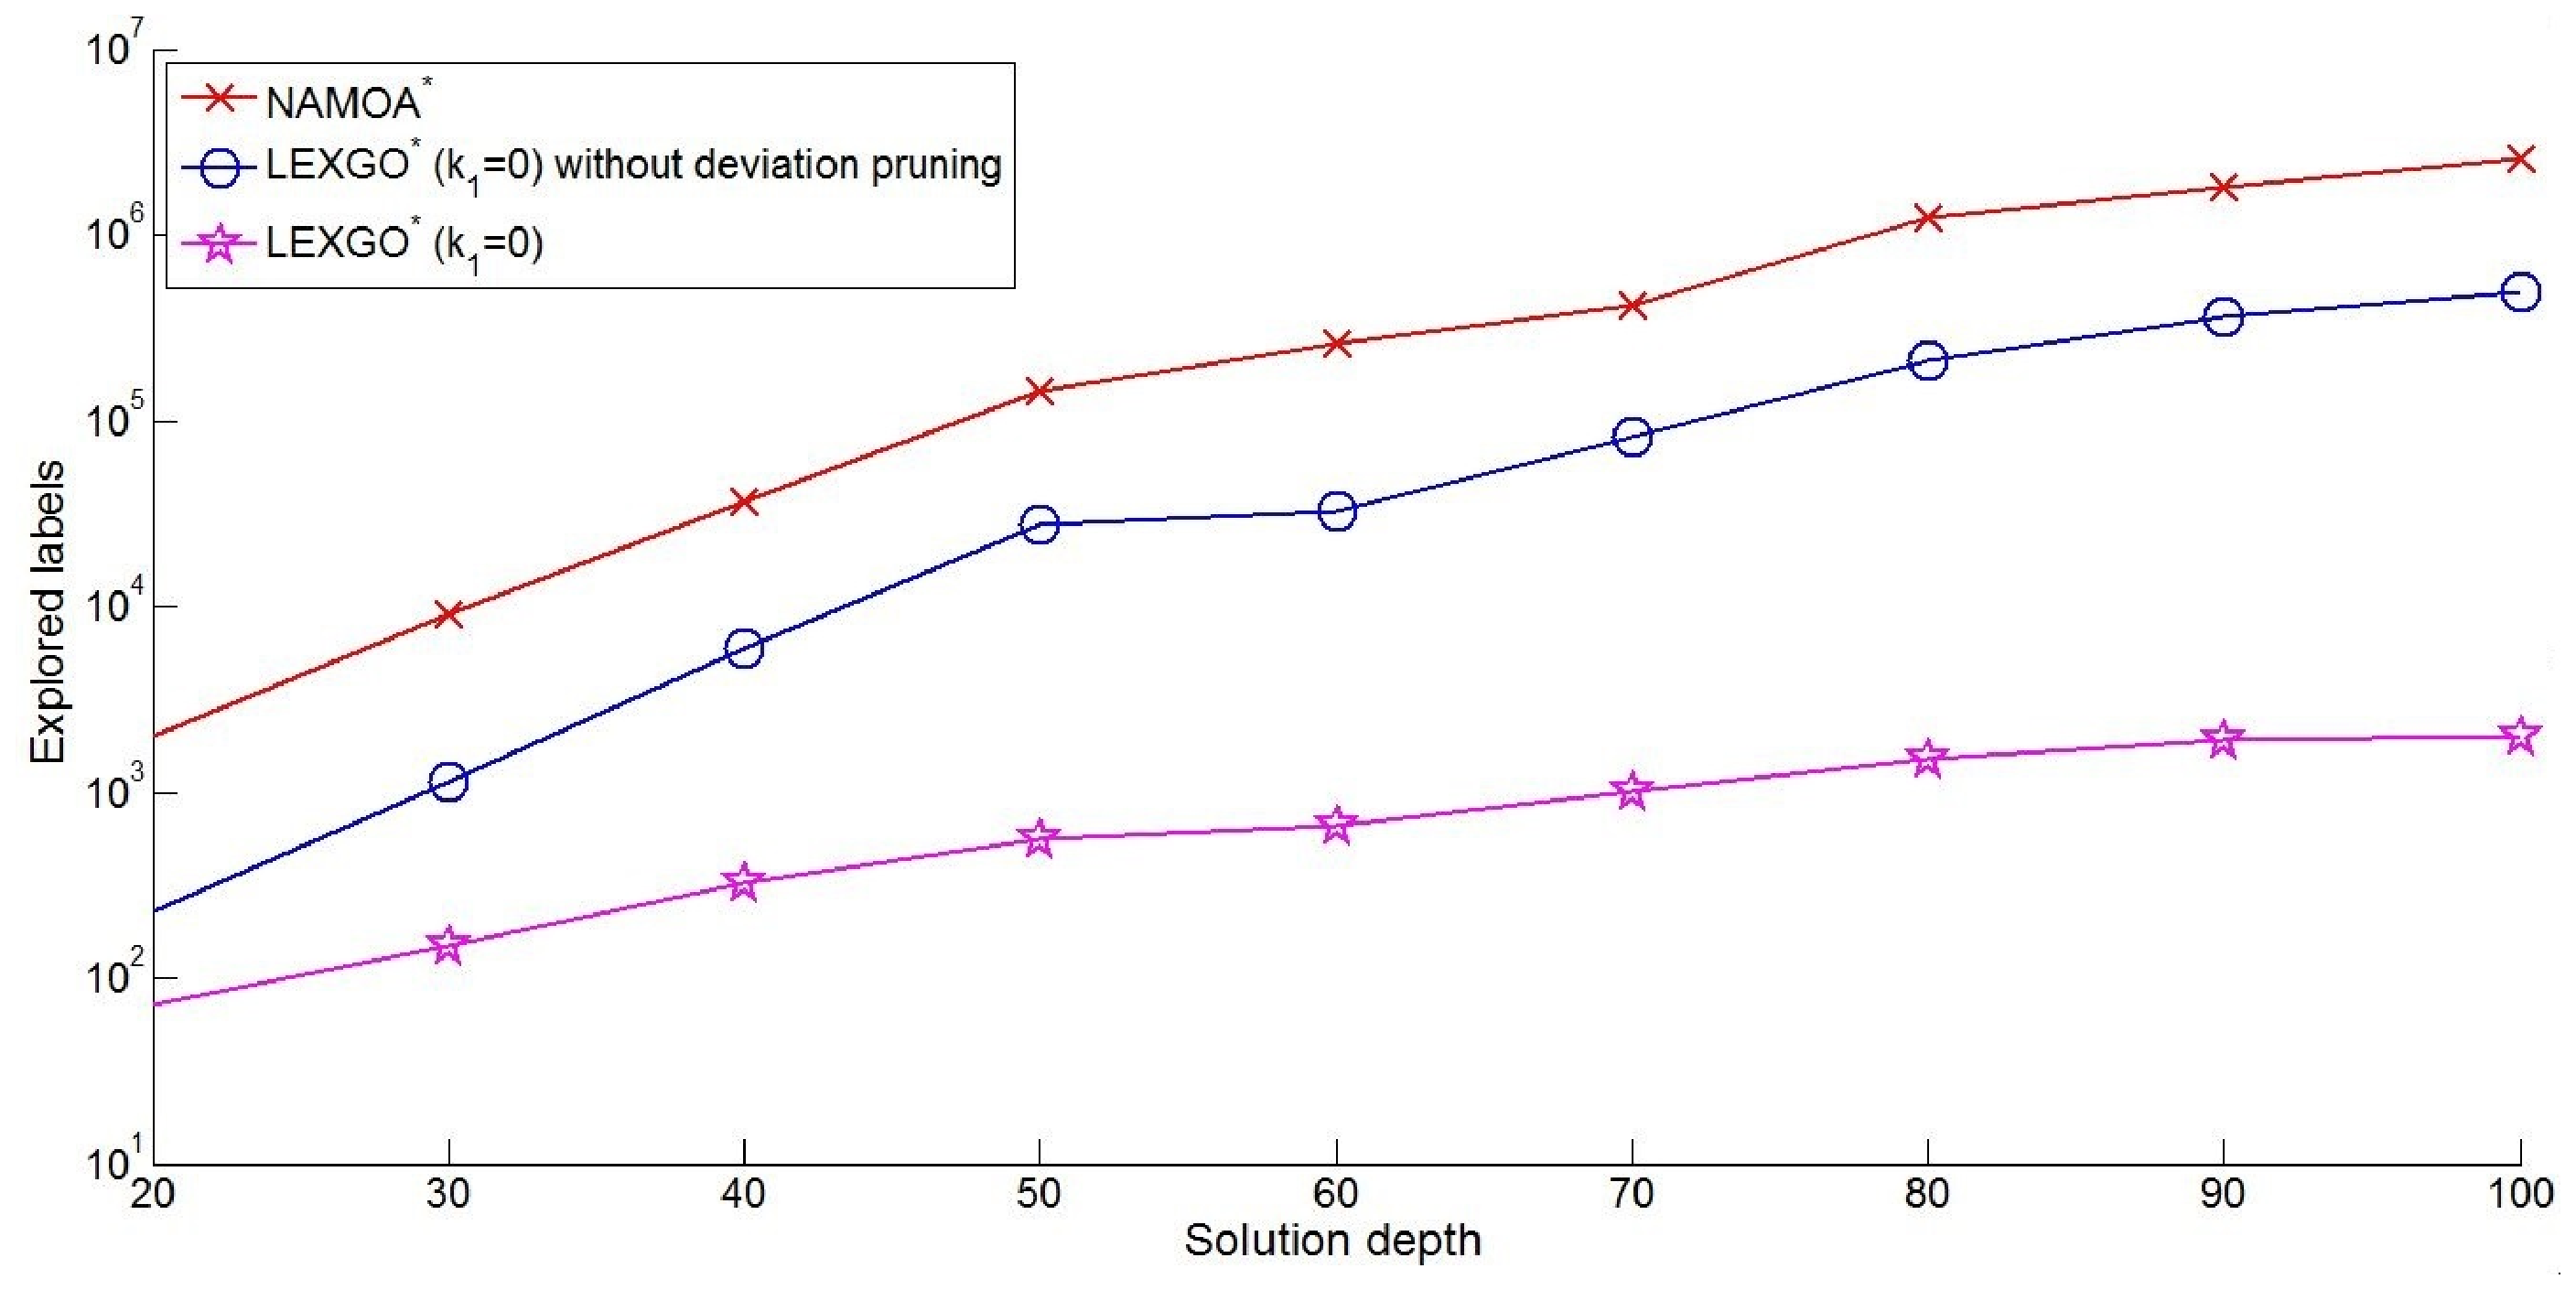
\includegraphics[width=1\textwidth]{Images/Chapter6/dev-pruning-labels0}
\caption{Class I experiments on grids, average explored labels per solution depth to \lexgo \ $(k_1 = 0)$ with and without deviation pruning.}
\label{fig:6-7}
\end{figure}

\begin{figure}
\centering
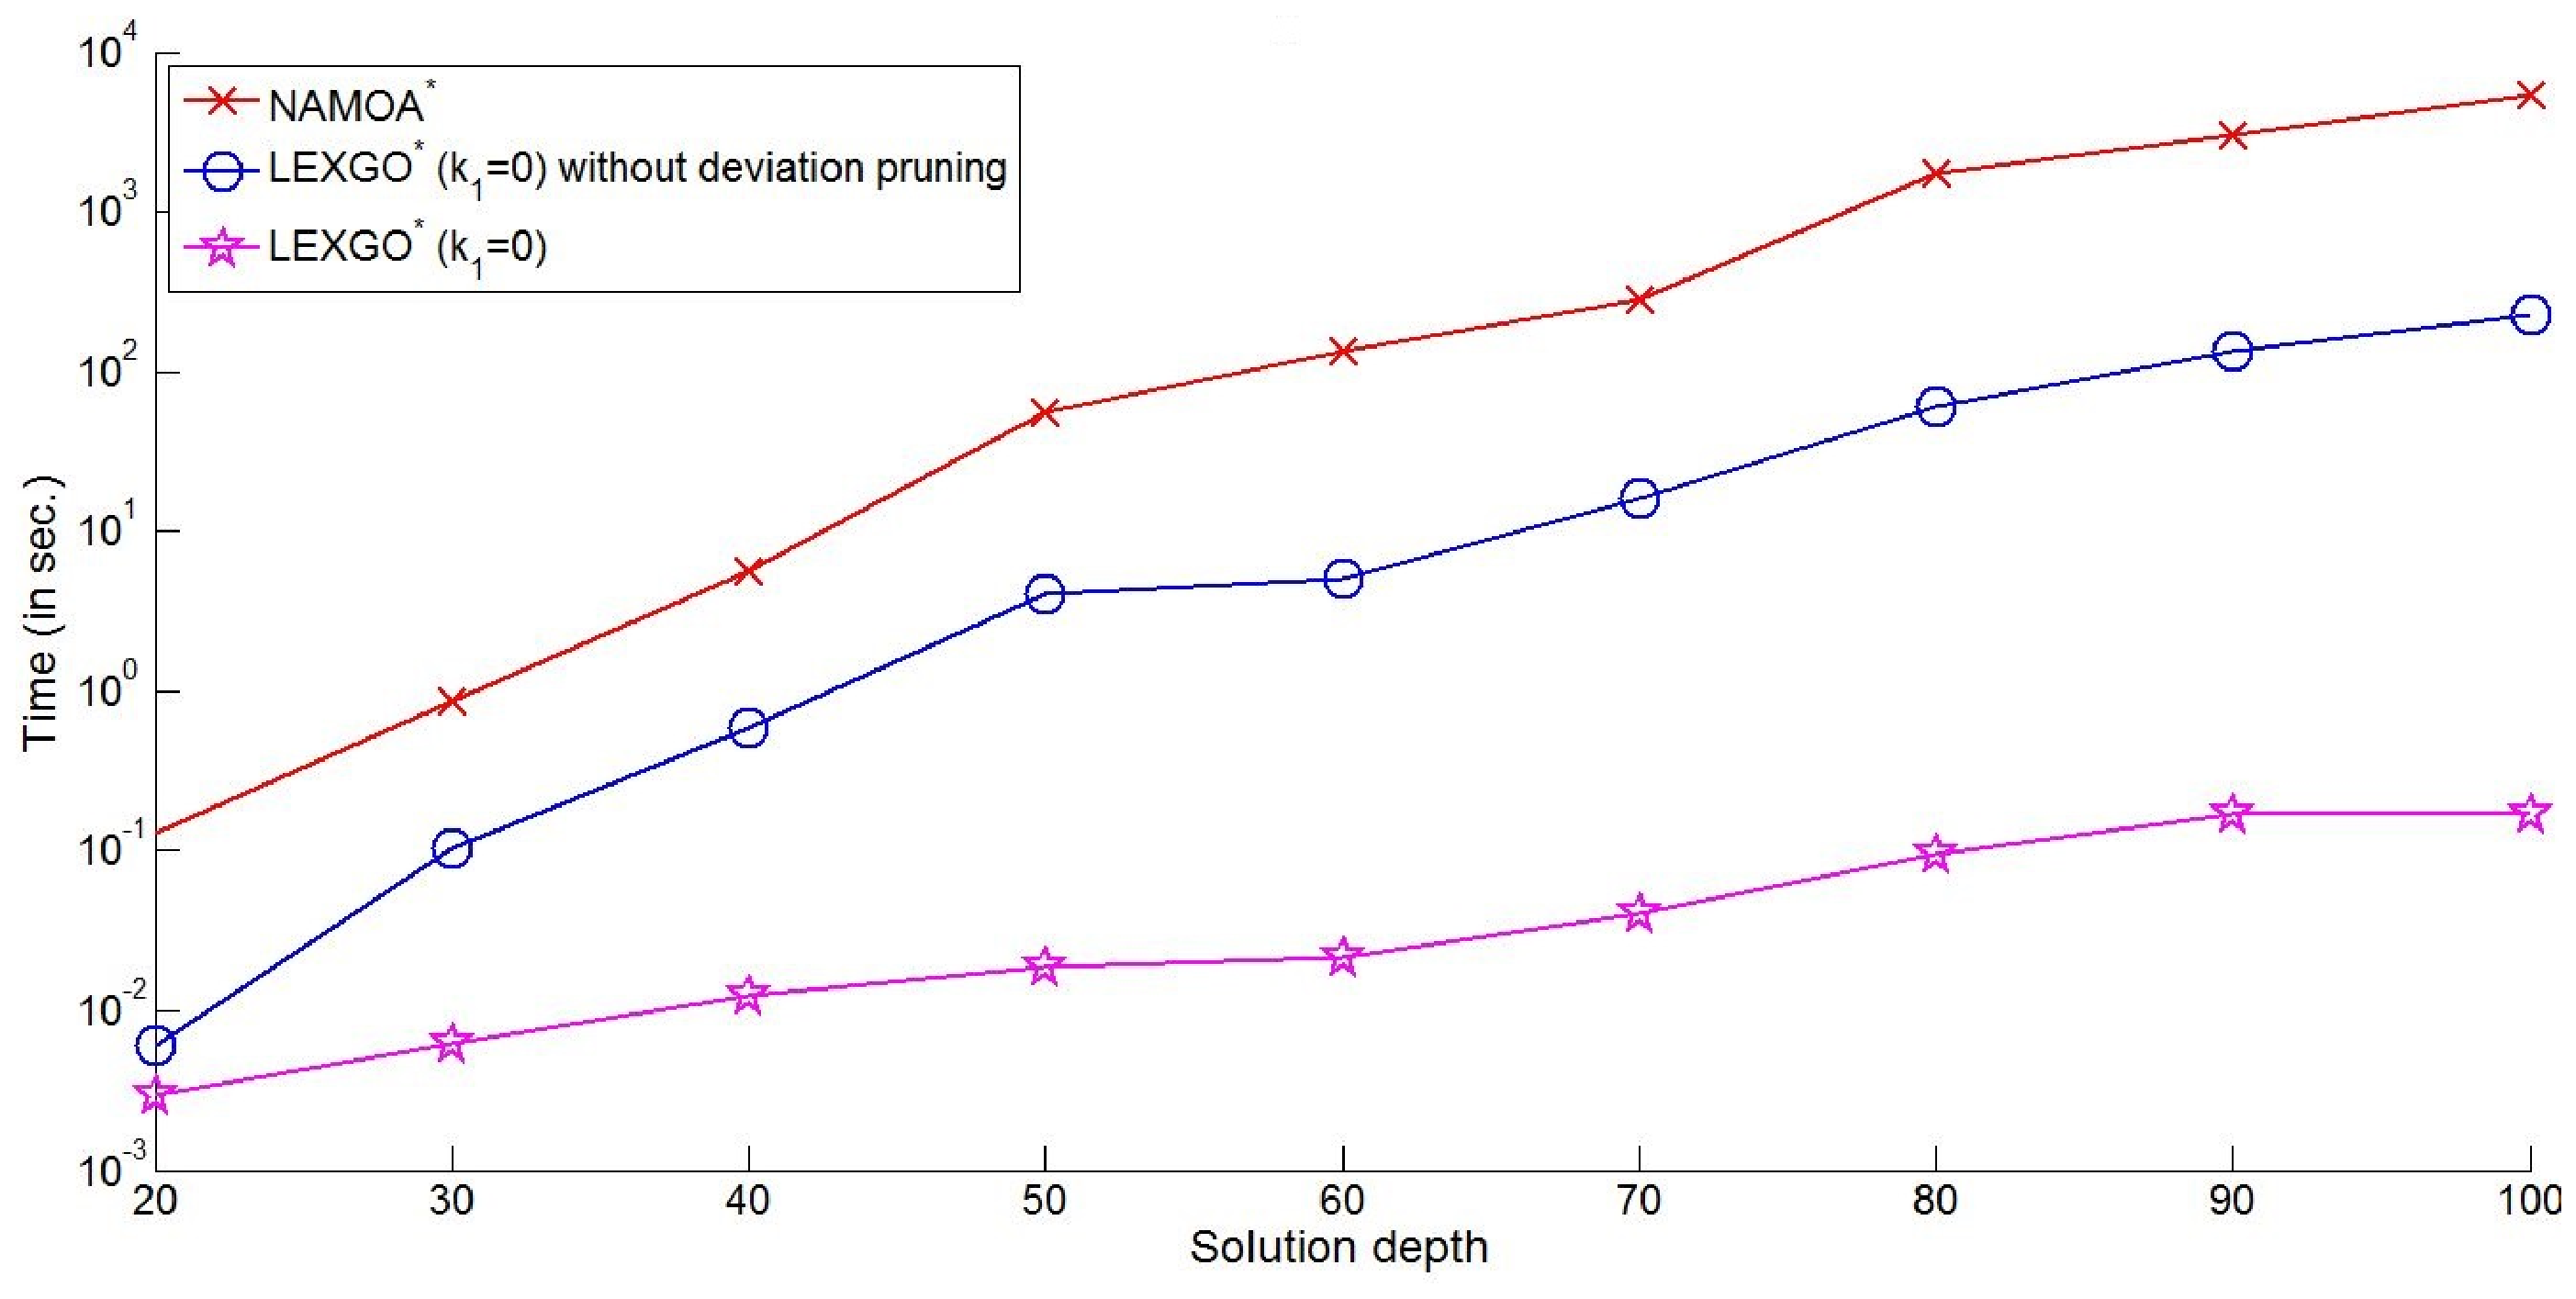
\includegraphics[width=1\textwidth]{Images/Chapter6/dev-pruning-exe0}
\caption{Class I experiments on grids, average runtimes in seconds per solution depth to \lexgo \ $(k_1 = 0)$ with and without deviation pruning.}
\label{fig:6-8}
\end{figure}

%-------------------------------------------------------------------
\subsection{Summary}
\label{chapEmpiricalAnalysis:subsec:summarygridslexgo}
%-------------------------------------------------------------------

We present a deeper study than the experiments already presented by the author in \citet{Pulido2014}. We have also added to the experimental set the linear aggregation order to both algorithms, \namoa \ and \lexgo, as well as $k_1=0.75$ for class II experiments. \namoalin \ outperforms \namoalex \ in all cases, by approximately a factor of two. Several studies have reported the same results for \namoa \ on the lexicographic and linear selection orders.  

Regarding \lexgolex \ and \lexgolin, the latter performs faster when the number of goal-optimal solution costs is bigger, i.e. when $k_1=\{1, 0.75\}$, by an approximate factor of 1.8, due to the fact that linear version finds the solutions at a later stage and therefore, a smaller number of filtering comparisons is needed. However, \lexgolex \ outperforms \lexgolin \ when the number of goal-optimal solution vectors is smaller, i.e. when $k_1=0.5$. Moreover, \lexgolex \ has a slightly better performance when goals cannot be satisfied, i.e. when $k_1=\{0.25, 0\}$. In the latter case, the relative performance is problem-dependent.

The comparative performance between \lexgolex \ vs \namoalex, and \lexgolin \ vs \namoalin \ turns out to be very similar in explored labels. However, the lexicographic order is comparatively more advantageous in runtime for \lexgo \ than the linear, having a smaller time overhead and better comparative performance. Even so, both \lexgo \ alternatives run faster than \namoa \ for $k_1=0.5$, they run several orders of magnitude faster for $k_1=0$ and around two orders of magnitude when $k_1=0.25$, regardless the selection order. 

%-------------------------------------------------------------------
\section{\texorpdfstring{\namoate}{NAMOA*dr} \ vs \texorpdfstring{\namoa}{NAMOA*}}
\label{chapEmpiricalAnalysis:sec:resultsgridsnamoate}
%-------------------------------------------------------------------

In this section, we analyze the runtime performance of two different versions of the \namoa \ algorithm: the standard version, and the newly introduced one. A description of these algorithms can be found in Sections \ref{chapMultiObjAlg:subsec:namoa} and \ref{chapMultiObjAlg:subsec:namoate}, respectively. \namoa \ and \namoate \ were presented in Section \ref{chapMultiObjAlg:subsec:namoa} and Section \ref{chapMultiObjAlg:subsec:namoate}, respectively. 

The experiments presented in this section analyze the impact of the dimensionality reduction technique on the sets of random grid problems previously used with $q=3$. Extra problem sets with $q=4$ and $q=5$ objectives have been added to the experimental evaluation of these algorithms. The solution depths considered for these new experiments are $d = \{20, 30, 40, 50 \}$ and $d = \{20, 30, 40 \}$ for $q=4$ and $q=5$, respectively.

These two versions of \namoa \ differ in the order of selection of OPEN labels and in the way dominance is checked in filtering and cl-pruning operations. The first analyzed variants are \namoalex \ and \namoalin, which use, to the best of our knowledge, the usual dominance pruning and filtering techniques in previously reported experimental evaluations of multiobjective search algorithms. The second algorithm analyzed, \namoate \ uses a lexicographic order of selection and the t-discarding technique for filtering and cl-pruning, as described in Section \ref{chapMultiObjAlg:sec:Time-efficient-MSalg}.

%-------------------------------------------------------------------
\subsection{Analysis}
\label{chapEmpiricalAnalysis:subsec:analysisgridsnamoate}
%-------------------------------------------------------------------

Table \ref{tab:6-6} shows the average size of relevant sets of labels for the execution of \namoate \ on random grid problems. The first column ($q$) indicates the number of objectives. The second column ($d$) displays solution depth. The third column (Max OPEN) displays the maximum cardinality of the set of open labels. The fourth column, $\sum G_{cl}$, displays the total number of closed (permanent) labels at termination, calculated as the sum of the number of labels at the $G_{cl}$ sets of all visited nodes. This is also the total number of labels expanded by the algorithm. The fifth column shows for comparison the sum of sizes of the corresponding sets of truncated labels, i.e. $\sum T(G_{cl})$. The sixth column displays the percentage ratio between columns four and five. For example, for $d = 20$, the average number of label expansions by \namoate \ was 1,985, while the average number of labels in the truncated sets was only 476, this results in a percentage ratio of 23.98\%.   

\begin{table}
\caption{Average size of relevant sets of labels for random grid problems solved by \namoate.}
\begin{center}
\begin{tabular}{crrrrrrrr}
\hline \noalign{\smallskip}
$q$ & $d$ & Max OPEN & $\sum G_{cl}$ & $\sum T(G_{cl})$ & \% & $\text{C}^*$ & $T(\text{C}^*)$ & \%\\
\noalign{\smallskip} \hline 
3 & 20  & 194    & 1,985     & 476    & 23.98 & 122   & 13  & 10.66 \\
3 & 30  & 723    & 9,164     & 2,091  & 22.82 & 302   & 32  & 10.60 \\
3 & 40  & 2,233  & 36,557    & 4,923  & 13.47 & 694   & 44  &  6.34 \\
3 & 50  & 8,327  & 145,823   & 12,450 &  8.54 & 1,599 & 60  &  3.75 \\
3 & 60  & 11,091 & 257,935   & 21,026 &  8.15 & 2,007 & 80  &  3.99 \\
3 & 70  & 17,312 & 420,056   & 29,845 &  7.11 & 2,561 & 74  &  2.89 \\
3 & 80  & 38,512 & 1,231,565 & 61,457 &  4.99 & 5,423 & 108 &  1.99 \\
3 & 90  & 51,817 & 1,789,607 & 81,036 &  4.53 & 5,912 & 122 &  2.06 \\
3 & 100 & 72,062 & 2,550,354 & 97,160 &  3.81 & 8,307 & 137 &  1.65 \\
\noalign{\smallskip}
4 & 20  & 531     & 6,192     & 2,061   & 33.28 & 493    & 83    & 16.83 \\
4 & 30  & 3,183   & 49,735    & 13,150  & 26.44 & 2,230  & 320   & 14.34 \\
4 & 40  & 14,409  & 283,811   & 44,191  & 15.57 & 7,826  & 774   &  9.89 \\
4 & 50  & 72,112  & 1,542,793 & 153,639 & 9.95  & 24,942 & 1,382 &  5.54 \\
\noalign{\smallskip}
5 & 20  & 1,127   & 15,681     & 6,539    & 41.70 & 1,819   & 522   & 28.69 \\
5 & 30  & 10,019  & 172,238    & 51,145   & 29.69 & 10,830  & 1,917 & 17.70 \\
5 & 40  & 62,280  & 1,371,885  & 319,333  & 23.27 & 49,634  & 8,320 & 16.76 \\
\hline
\end{tabular} 
\end{center}
\label{tab:6-6}
\end{table}

Column 7 in Table \ref{tab:6-6} shows the average number of different non-dominated solution vectors in COSTS ($\text{C}^*$). The eighth column displays the size of the corresponding truncated set $T(\text{C}^*)$. The last column displays the percentage ratio between columns six and seven. 

Table \ref{tab:6-7} displays the average runtimes of the three considered alternatives of \namoa \ with $q \in \{3,4,5\}$ objectives for random grid problems. The last columns show the relative percentage improvement of \namoate \ over \namoalex \ and \namoalin, respectively.

\begin{table}
\caption{Average runtimes in seconds for random grid problems.}
\begin{center}
\scalebox{.80}{
\begin{tabular}{crrrrrrrrr}
\hline \noalign{\smallskip}
$q$ & $d$ & \namoalex & $\sigma_{lex}$ & \namoalin & $\sigma_{lin}$ & \namoate & $\sigma_{dr}$ & $(\frac{dr}{lex})$\% & $(\frac{dr}{lin})$\% \\
\noalign{\smallskip} \hline 
3 & 20  & 0.06  & 0.02    & 0.04  & 0.01 & 0.0622  & 0.01 & 99.67 & 132.91 \\
3 & 30  & 0.46   & 0.26     & 0.36   & 0.18 & 0.293    & 0.11 & 62.74 & 80.23 \\
3 & 40  & 3.53    & 1.21     & 2.36    & 0.74 & 1.32     & 0.30 & 37.39 & 56.13 \\
3 & 50  & 36.83   & 15.56    & 18.37   & 5.67 & 6.87     & 2.02 & 18.65 & 37.41 \\
3 & 60  & 86.93   & 49.57    & 43.83   & 22.94 & 11.94   & 4.48 & 13.73 & 27.26 \\
3 & 70  & 178.53  & 106.75   & 83.37   & 47.77 & 20.93   & 7.69 & 11.72 & 25.11 \\
3 & 80  & 1,164.11 & 293.72   & 533.79  & 135.96 & 76.01  & 14.22 & 6.52 & 14.24 \\
3 & 90  & 2,030.06 & 730.05   & 981.32  & 313.79 & 120.66 & 33.19 & 5.94 & 12.30 \\
3 & 100 & 3,662.93 & 1,100.91 & 1,754.43 & 583.28 & 196.13 & 52.74 & 5.35 & 11.18 \\
\noalign{\smallskip}
4 & 20  & 0.39   & 0.14     & 0.30    & 0.11     & 0.23   & 0.07 & 58.52 & 76.66 \\    
4 & 30  & 11.64   & 4.22     & 8.88    & 3.87     & 4.31   & 1.97 & 37.02 & 48.53 \\     
4 & 40  & 292.17  & 188.27   & 166.36  & 105.31   & 50.41  & 29.47 & 17.25 & 30.30 \\     
4 & 50  & 5,604.29 & 2,356.35 & 3,173.81 & 1,171.11 & 645.37 & 195.84 & 11.51 & 20.33 \\
\noalign{\smallskip}
5 & 20  & 4.01     & 1.51     & 2.99     & 1.14     & 2.20    & 0.76 &  54.86 & 73.57 \\  
5 & 30  & 204.69   & 135.77   & 114.91   & 73.32    & 57.89   & 34.61 &  28.28 & 50.37 \\    
5 & 40  & 10,848.24 & 7,404.86 & 6,141.63  & 4,212.81 & 1,919.56 & 1,269.98 &  17.69 & 31.25 \\ 
\hline
\end{tabular} 
}
\end{center}
\label{tab:6-7}
\end{table} 

All evaluated algorithms perform op-pruning in the same way. However, \namoate \ uses a different technique for cl-pruning and filtering. Figure \ref{fig:6-9} displays some results of the execution of \namoate: the percentage of labels pruned by $G_{op}$ (op-pruning), truncated closed node labels $T(G_{cl})$ (cl-pruning), and filtered by  $T(\text{C}^*)$ over the total number of discarded labels. Results are displayed as a function of solution depth $d$, (a) for $q=3$ objectives, (b) for $q=4$ objectives, and (c) for $q=5$ objectives. 

\begin{figure}
    \begin{center}
%
      \subfigure[$q = 3$]{%
            \label{fig:6-9a}
        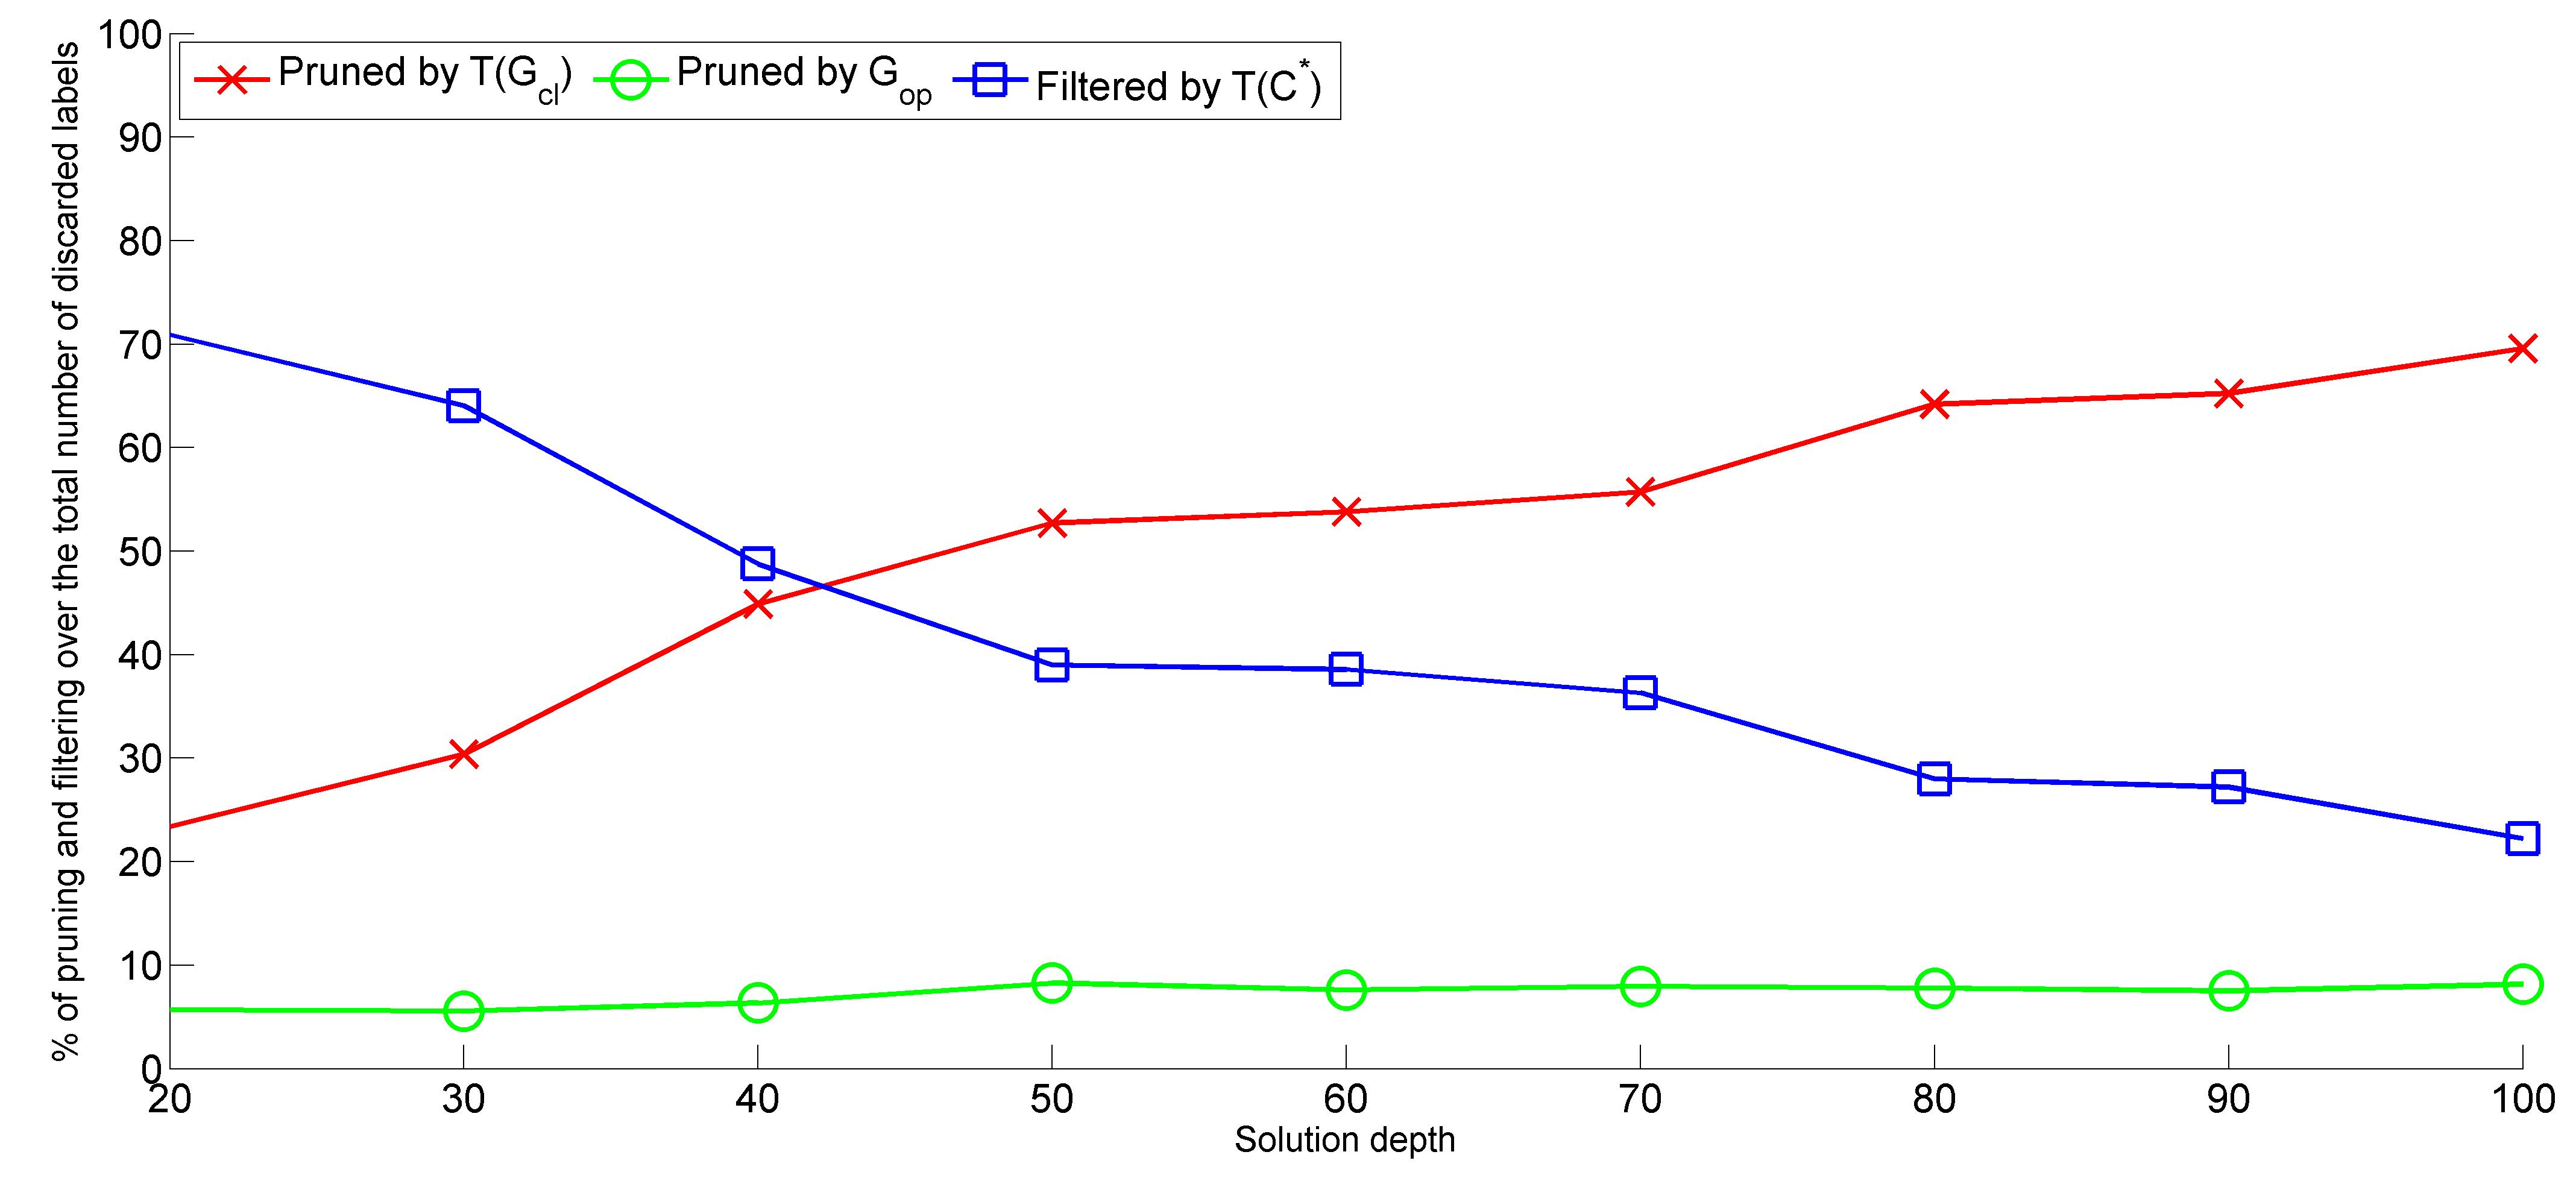
\includegraphics[width=0.95\textwidth]{Images/Chapter6/pruned-filtered-labels-grids-perc-a}
        }\\ %  ------- End of the first row ----------------------%
      \subfigure[$q = 
            4$]{%
       		\label{fig:6-9b}  
 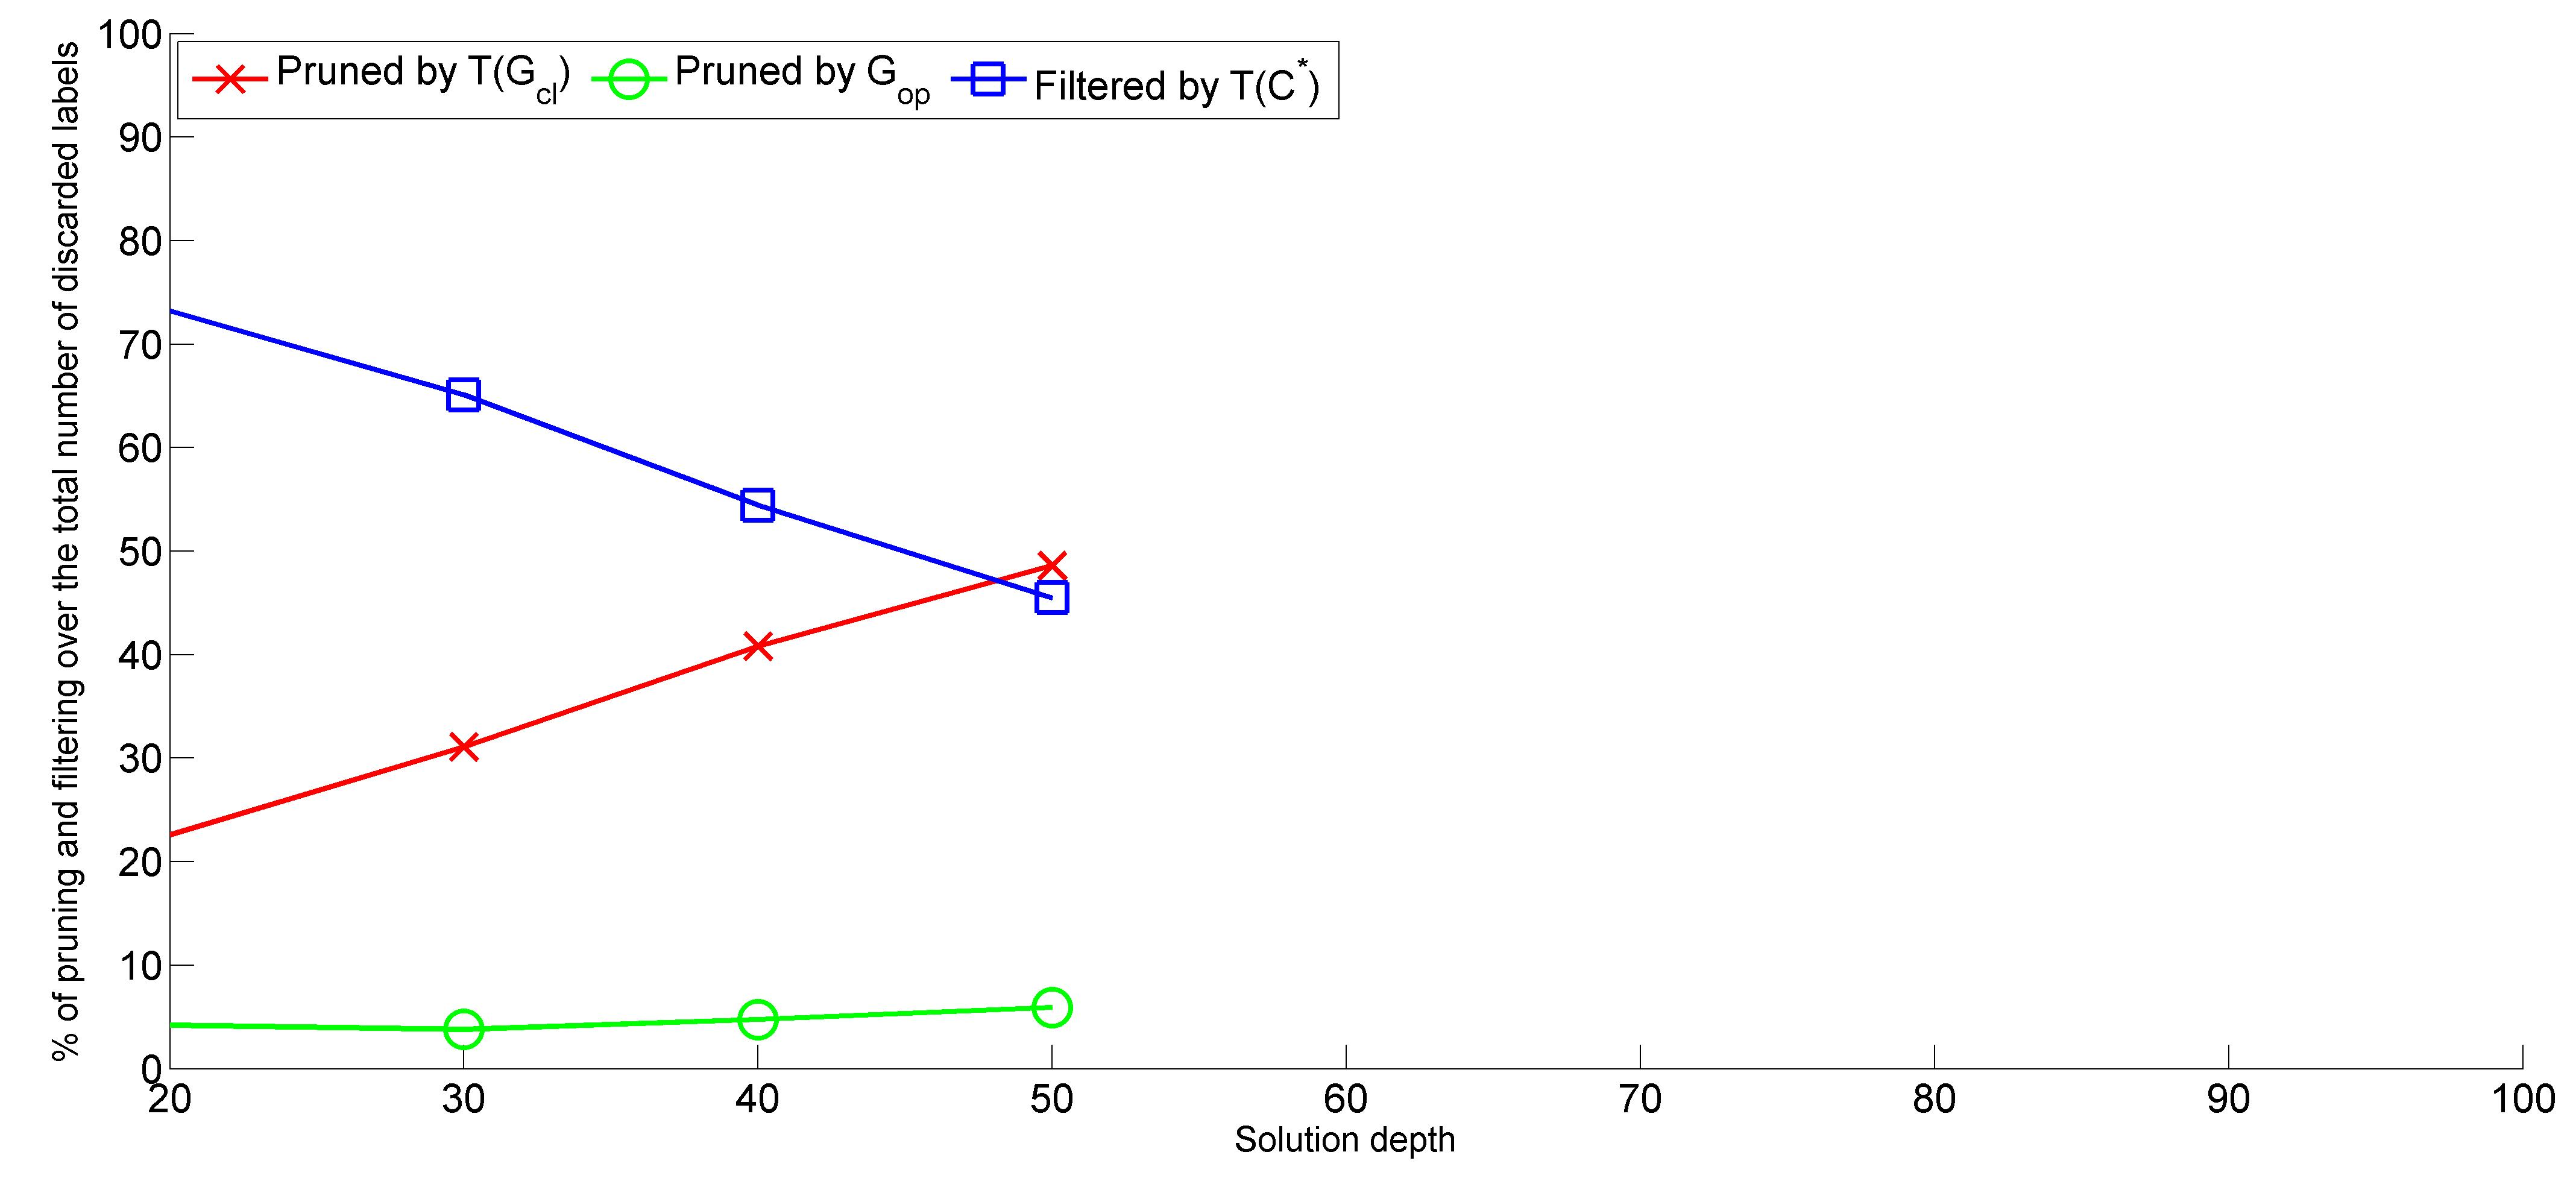
\includegraphics[width=0.95\textwidth]{Images/Chapter6/pruned-filtered-labels-grids-perc-b}
        }\\ %  ------- End of the first row ----------------------%
      \subfigure[$q = 5$]{%
            \label{fig:6-9c}
        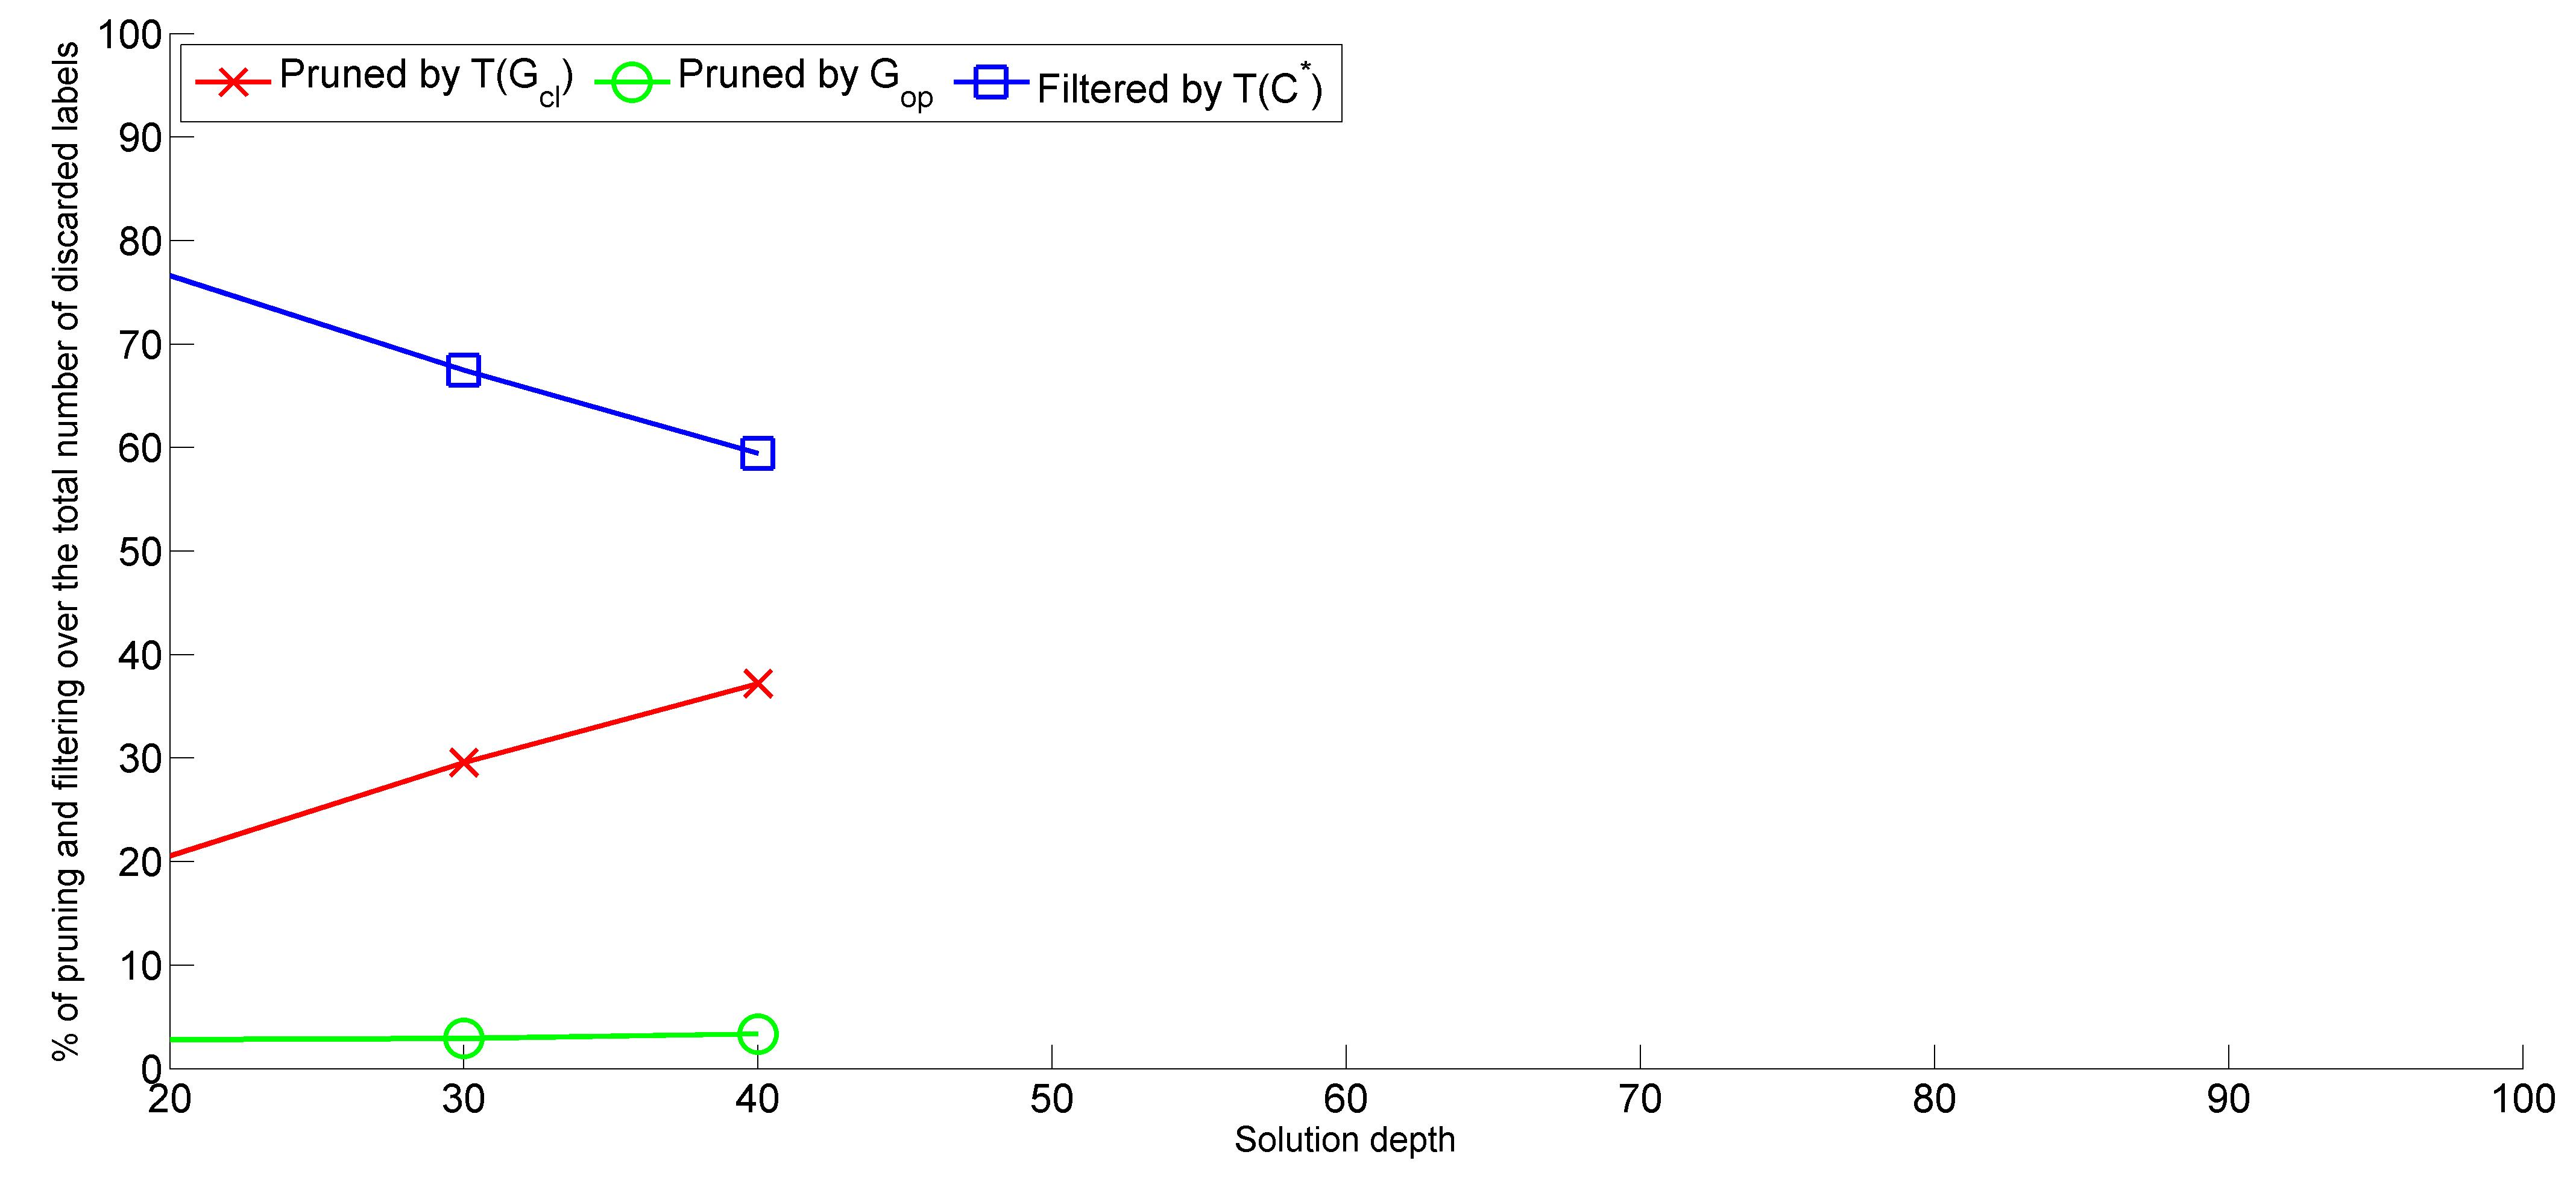
\includegraphics[width=0.95\textwidth]{Images/Chapter6/pruned-filtered-labels-grids-perc-c}
      }%
    \end{center}
    \vspace{-0.25in} 
    \caption{%
Percentage of pruned and filtered labels over the total number of discarded labels by \namoate \ per solution depth for $q \in \{3,4,5\}$ objectives in grid problems.  
    }%
    \label{fig:6-9}

\end{figure}

Figure \ref{fig:6-10} shows runtimes of \namoalex, \ \namoalin \ and \namoate \ in logarithmic scale against solution depth for $q=\{3,4,5\}$ objectives. The items in the legend indicate the version of the algorithm and the objectives, e.g. dr(4) indicates \namoate \ with $q=4$. Finally, Figure \ref{fig:6-11} displays the percentage of runtimes of \namoate \ and \namoalin \ over \namoalex \ for $q = 3$ experiments displayed as a function of solution depth. 

\begin{figure}%[ht]
\centering
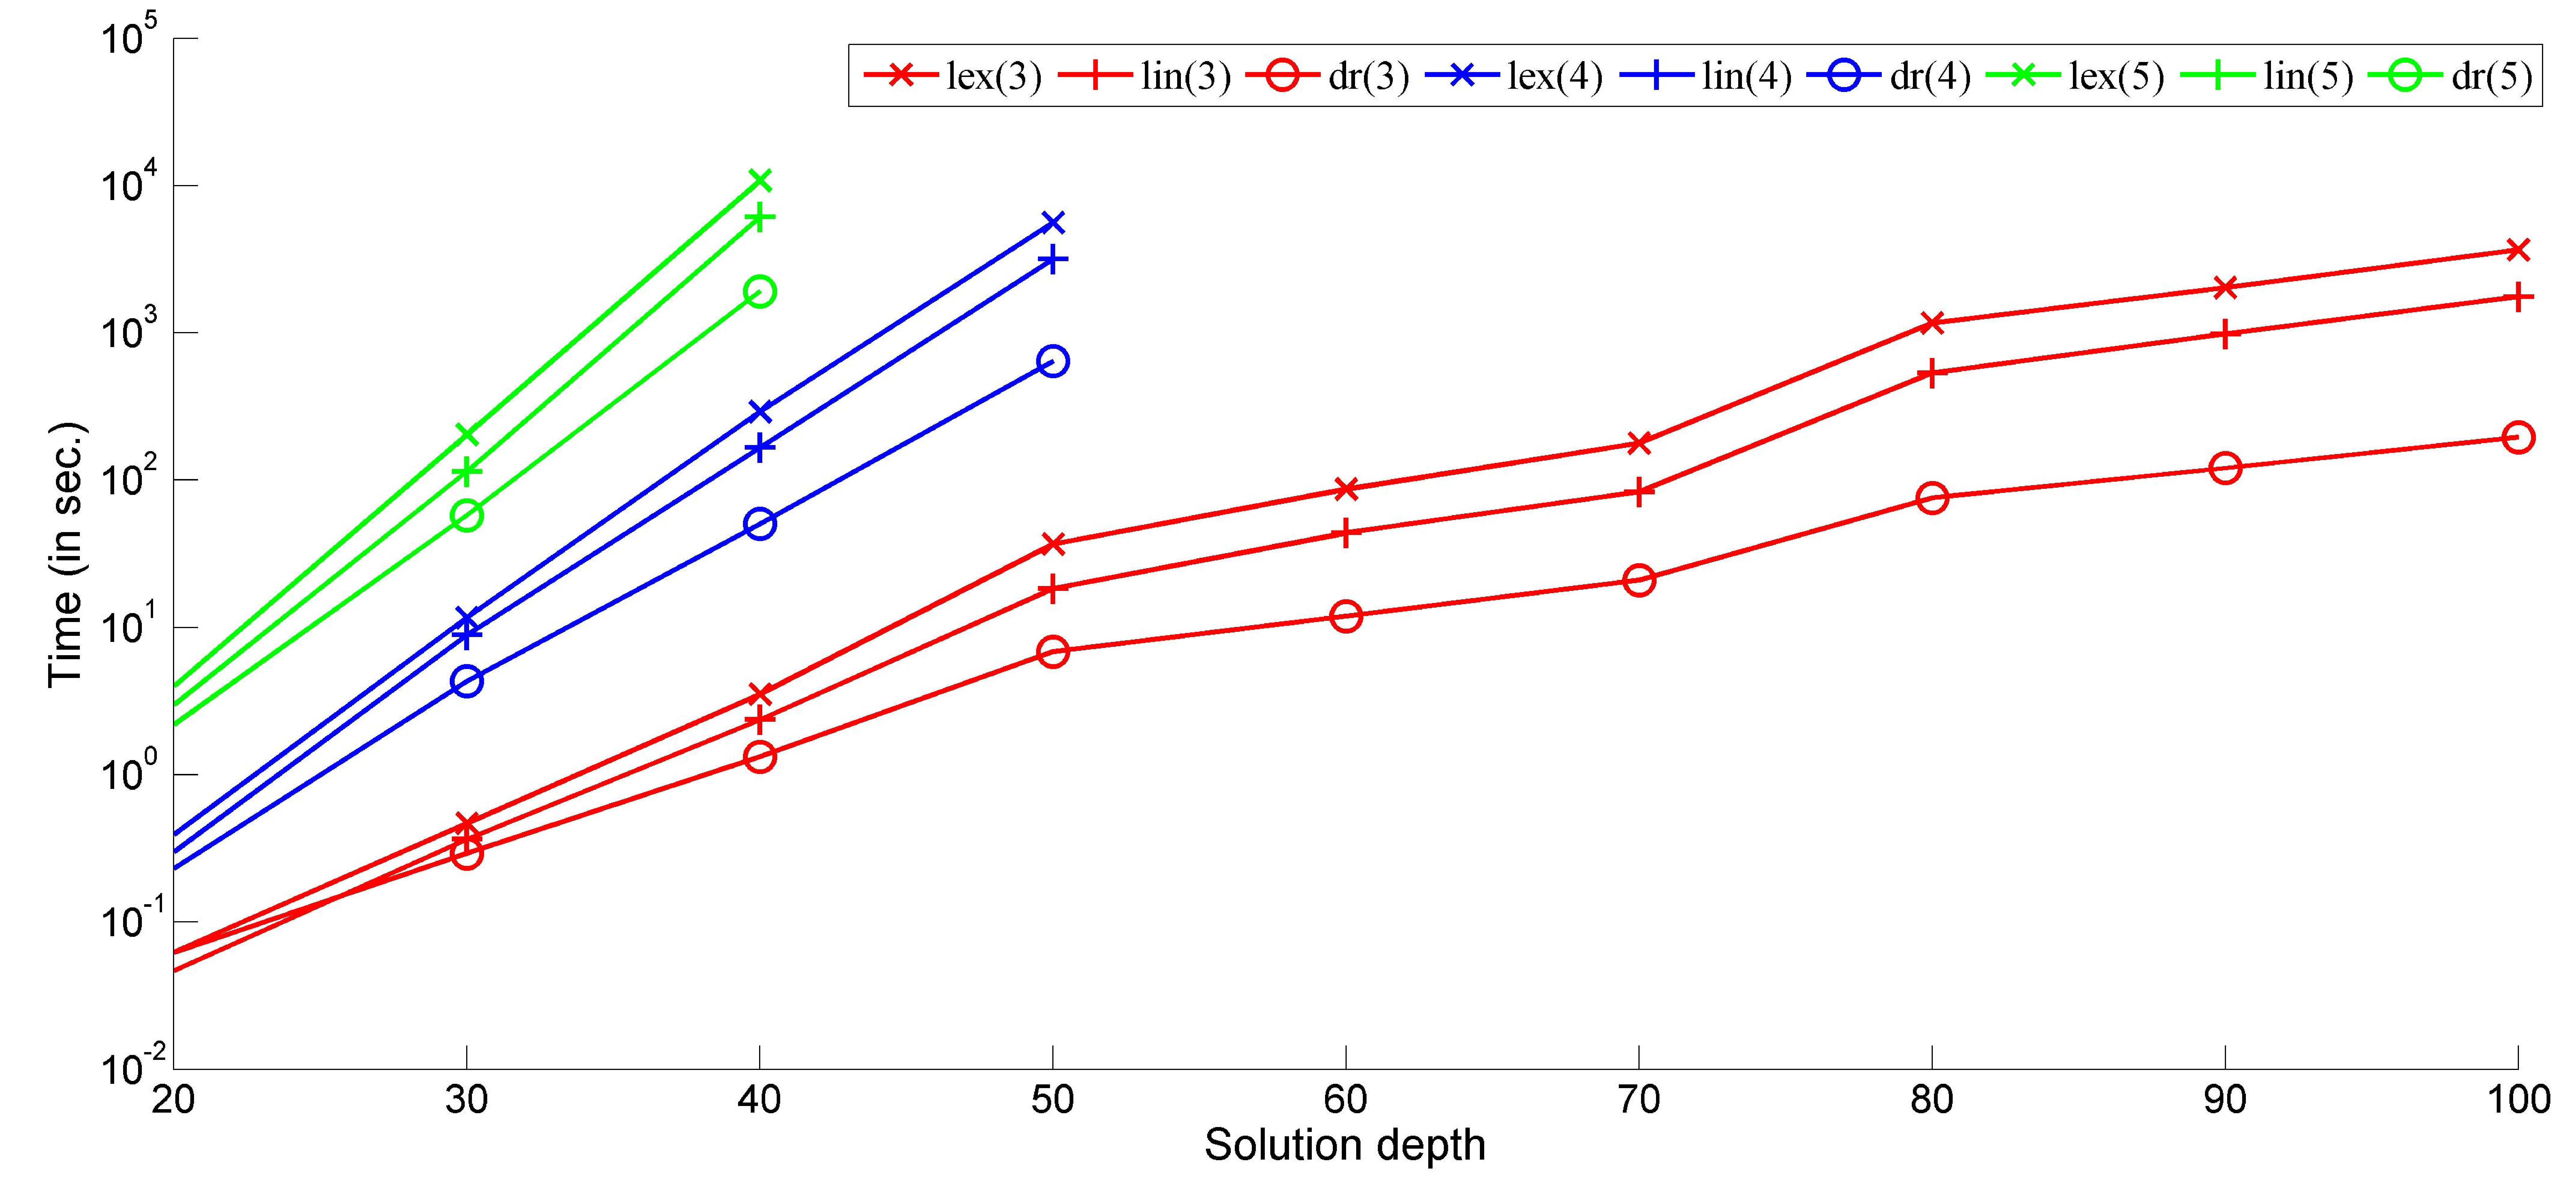
\includegraphics[width=1\textwidth]{Images/Chapter6/exe-time-grids-namoas}
\caption{Average runtimes for $q \in  \{3,4,5\}$ objectives per solution depth in grid problems.}
\label{fig:6-10}
\end{figure}

\begin{figure}%[ht]
\centering
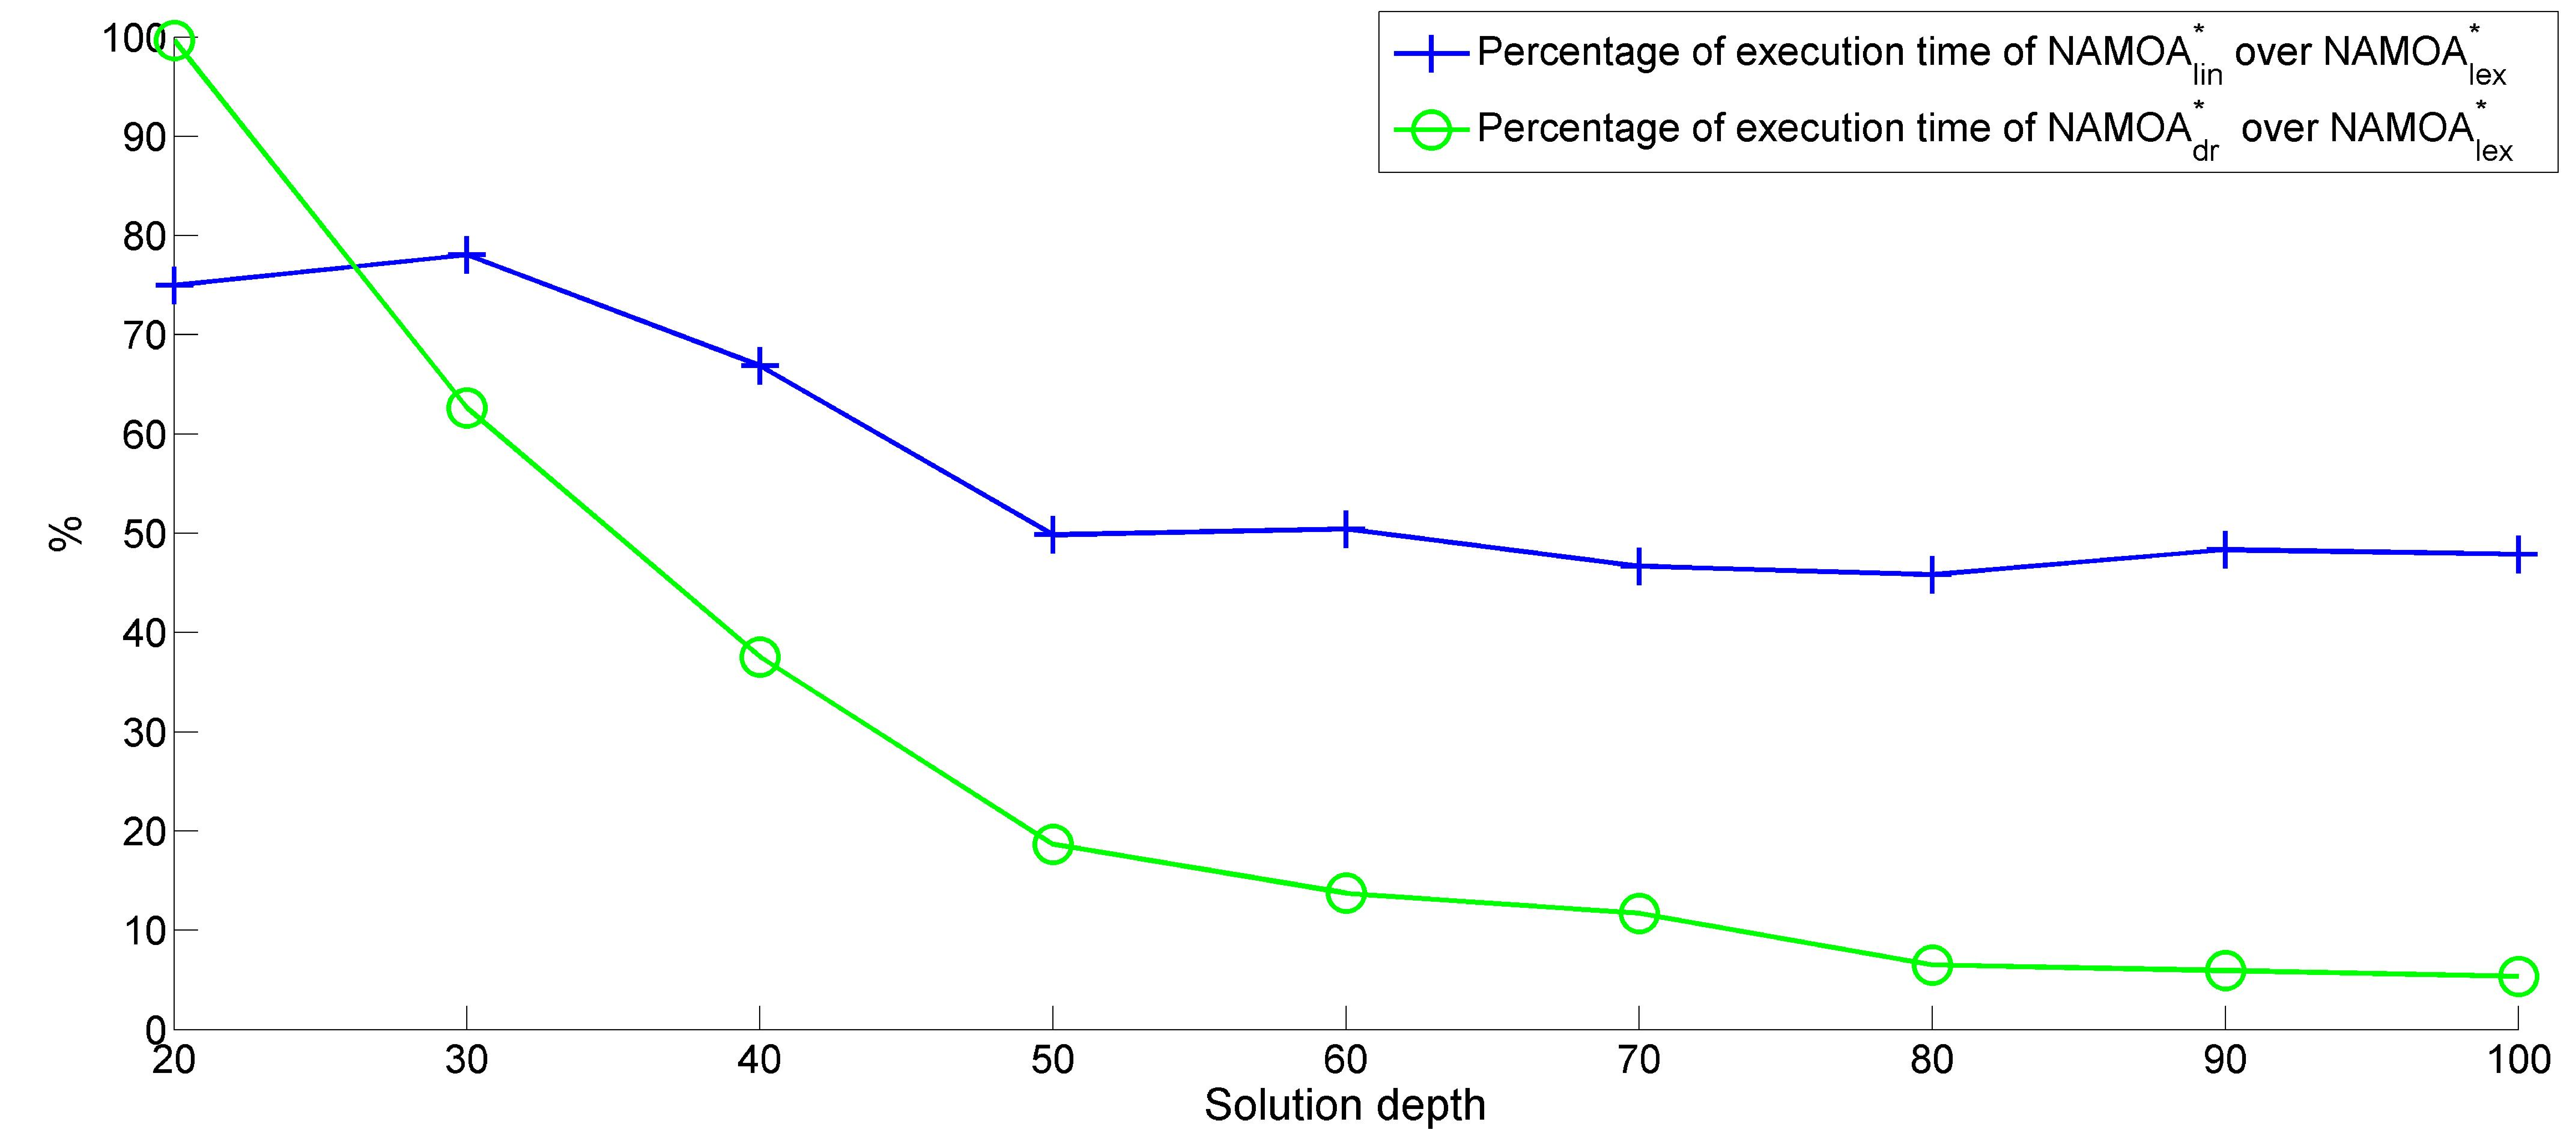
\includegraphics[width=1\textwidth]{Images/Chapter6/perc-exe-time-grids-namoas}
\caption{Percentage of average runtime of \namoate \ and \namoalin \ over \namoalex \ for $q = 3$ grid problems.}
\label{fig:6-11}
\end{figure}

%-------------------------------------------------------------------
\subsection{Summary}
\label{chapEmpiricalAnalysis:subsec:summarygridsnamoate}
%-------------------------------------------------------------------

A linear aggregation selection function is consistently more efficient in runtime than a lexicographic function when both are applied to standard \namoa. However, the lexicographic order can be exploited by the t-discarding technique for filtering and cl-pruning (\namoate). Results over grid problems reveal a dramatic improvement in runtime performance of over an order of magnitude for three-objective problems (see Figure \ref{fig:6-10}). The speedup of \namoate \ over \namoalex \ and \namoalin \ even grows with problem difficulty (see Table \ref{tab:6-7} and Figure \ref{fig:6-11}), reducing time requirements over 90\% for the harder $q = 3$ problems. When more objectives are considered, $q=\{4,5\}$, similar results can be observed, although a smaller number of experiments can be presented due to the increasing computational difficulty.  

As expected, multiobjective label-setting search spends most of the time performing dominance checks between labels. Every new label has to be checked for op-pruning, cl-pruning, and filtering. Figure \ref{fig:6-9} shows that, for the harder grid problems, cl-pruning is the operation that tends to discard most labels for deeper solutions. The same tendency can be observed regardless the number of objectives. 

While the ratio of labels discarded by filtering decreases with problem difficulty, it was always larger than the ratio of those discarded by op-pruning in our grid experiments. This is important for the efficiency of \namoate, since cl-pruning and filtering can both benefit from t-discarding. Table \ref{tab:6-6} reveals that the truncated sets of labels used by t-discarding are significantly smaller than the original ones, and their relative size even decreases with problem difficulty. For example, with solution depth $d = 100$ and $q = 3$, a label is checked against a set of 8,307 labels for filtering in the worst case with the standard procedure, while with t-discarding the worst case involves only a set of 137 labels (or 1.65\%). 

%-------------------------------------------------------------------
\section{\texorpdfstring{\lexgote}{LEXGO*dr} \ vs \texorpdfstring{\lexgo}{LEXGO*}}
\label{chapEmpiricalAnalysis:sec:resultsgridslexgote}
%-------------------------------------------------------------------

In this section we examine the performance of the dimensionality reduction technique applied to \lexgo, called \lexgote. A detailed description of \lexgo \ and \lexgote \ are presented in Section \ref{chapMultiObjAlg:subsec:lexgo} and Section \ref{chapMultiObjAlg:subsec:lexgote}, respectively. The experiments presented below are applied to the random grid problems with three objectives and goals defined in Section \ref{chapEmpiricalAnalysis:sec:grids}.

%-------------------------------------------------------------------
\subsection{Analysis on class I experiments}
\label{chapEmpiricalAnalysis:subsec:analysisgridslexgotec1}
%-------------------------------------------------------------------

Table \ref{tab:6-8} displays average runtimes for \lexgolex, \lexgolin, and \lexgote \ for depth $d = 100$. The last column shows the speed-up obtained by \lexgote \ over the best version of standard \lexgo \ for each value of $k_1$. \lexgote \ achieves important reductions in runtime when goals can be satisfied, i.e. when $k_1=\{1, 0.75, 0.5\}$ and it barely affects runtimes when goals cannot be satisfied, i.e. $k_1=\{0.25, 0\}$. Figure \ref{fig:6-12} shows graphically the relative runtime performance of \lexgote \ over the best previous runtimes of \lexgo, as a function of solution depth. Values corresponding to $k_1=0$ are not shown since they are practically zero. 

\begin{table}
\caption{Class I experiments on grids, average runtimes in seconds of \lexgolex, \lexgolin \ and \lexgote \ for $d = 100$. Speed-up of \lexgote \ over the best standard version of \lexgo.}
\centering
\begin{tabular}{rrrrr}
\cline{2-5} \noalign{\smallskip}
$k_1$ & \lexgolex & \lexgolin & \lexgote & Speedup\\
\noalign{\smallskip} \hline
1 & 3,763.78 & 2,114.18 & 254.40 & 8.31 \\
0.75 & 3,381.33 & 1,847.88 & 300.86 & 6.14\\
0.5 & 819.28 & 1,145.15 & 282.49 & 2.90 \\
0.25 & 33.47 & 37.45 & 35.37 & 0.94 \\
0 & 0.07 & 0.09 & 0.10 & 0.77\\
\hline
\end{tabular}
\label{tab:6-8}
\end{table}

\begin{figure}%[!ht]
\centering
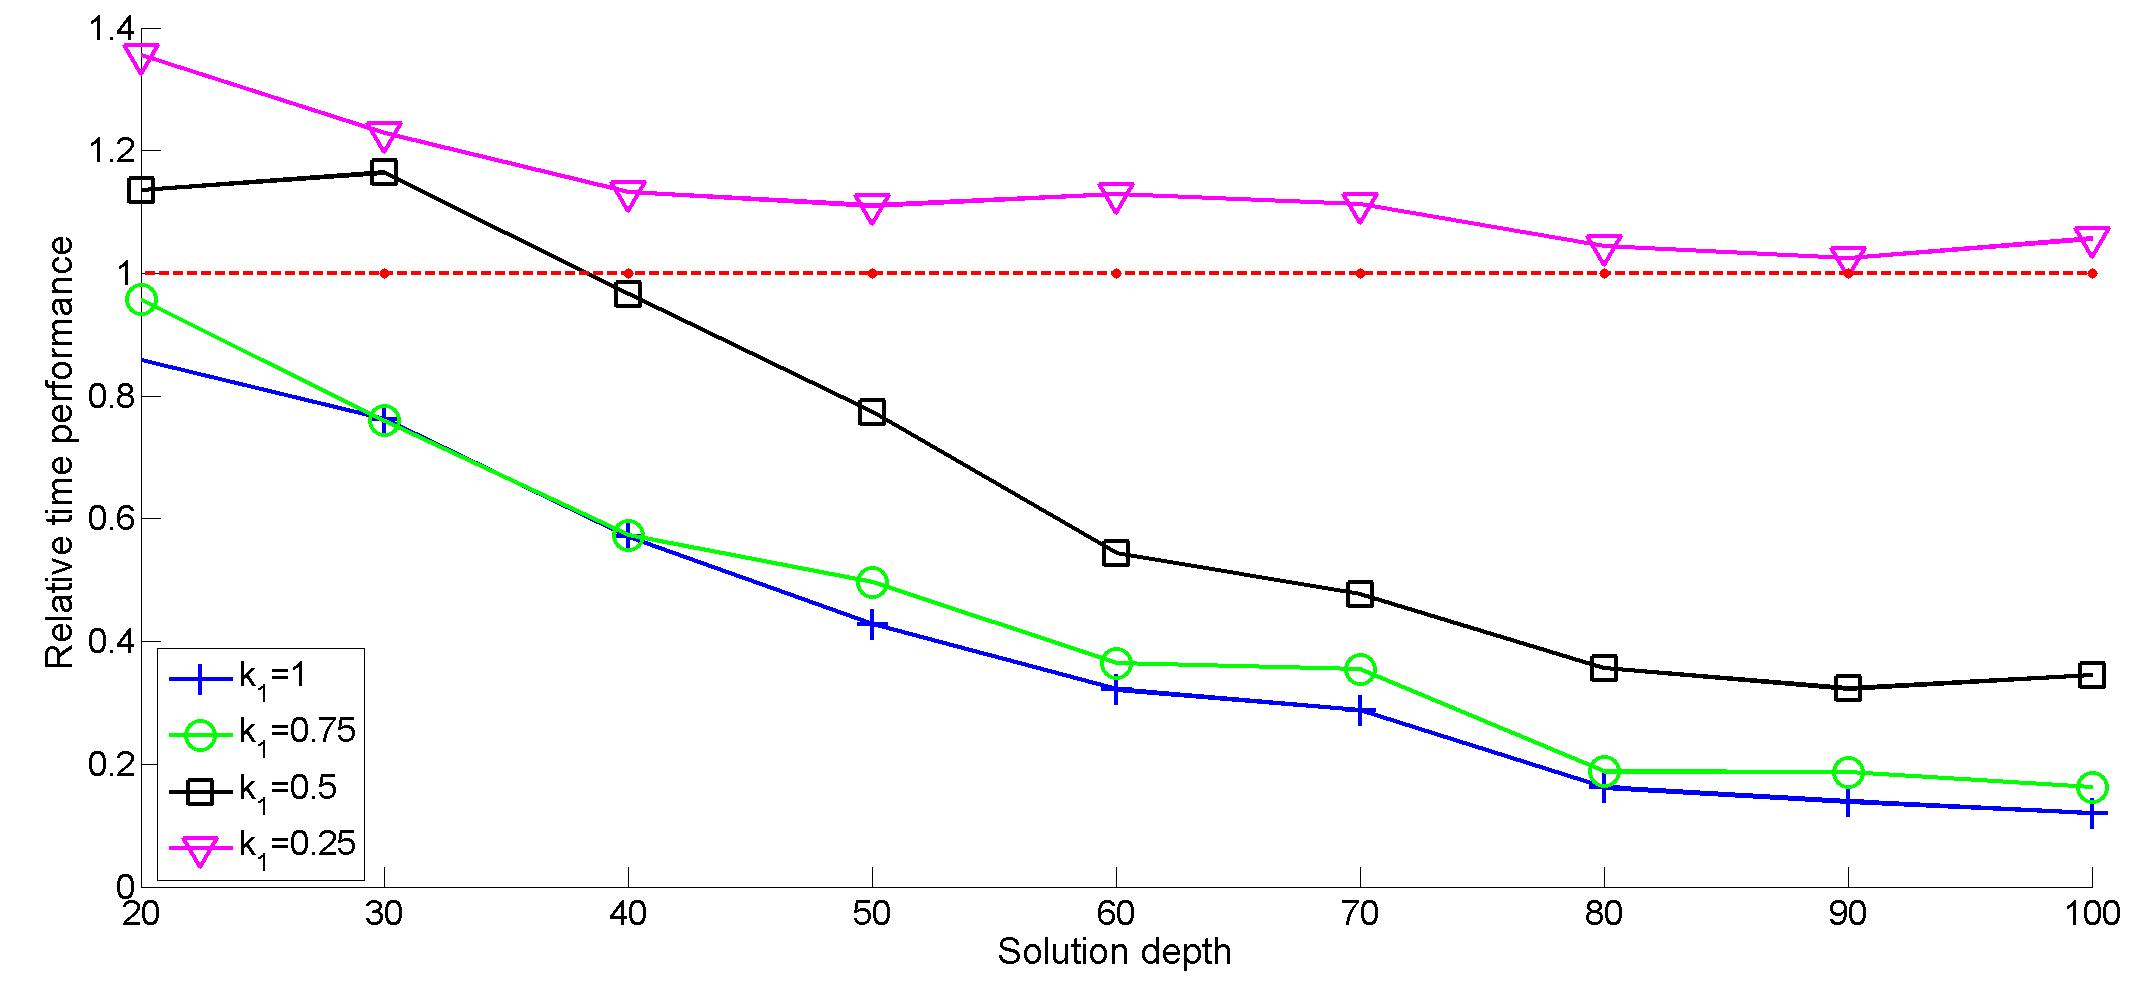
\includegraphics[width=1\textwidth]{Images/Chapter6/class1-exe-time-lexgo-te}
\caption{Class I experiments on grids, relative runtime performance of \lexgote \ over the best runtimes of standard \lexgo.}
\label{fig:6-12}
\end{figure}

%-------------------------------------------------------------------
\subsection{Analysis on class II experiments}
\label{chapEmpiricalAnalysis:subsec:analysisgridslexgotec2}
%-------------------------------------------------------------------

Table \ref{tab:6-9} shows the average runtimes of \lexgote \ for all possible values of $k_2$ with  $k_1=0.75$ and $k_1=0.5$. Figures \ref{fig:6-13a} and \ref{fig:6-13b} display, as a function of solution depth, the relative runtime performance of \lexgote \ over the best previous runtimes of \lexgo \ in $k_1=0.75$ and $k_1=0.5$, respectively.

Just as in the case of class I experiments, \lexgote \ obtains a better efficiency when the number of goal-optimal solution costs is greater. Thus, the relative runtime for $k_1=0.75$ is around 20\% and for $k_1=0.5$ around 30\% to 70\% of \lexgolin, the fastest version of the \lexgo \ algorithm so far. The sole case when \lexgote \ does not show improvement in practice is when  $k_1=0.5$ and  $k_2=0.125$. We can observe in Table \ref{tab:6-3} that in this case the goals are rarely satisfied by any problem instance.

\begin{table}
\caption{Class II experiments on grids, \lexgote \ runtimes in seconds.}
\centering
\begin{tabular}{rrrrrrrrrr}
\hline \noalign{\smallskip}
 & \multicolumn{8}{c}{\lexgote} & \\
\noalign{\smallskip} \cline{2-9}
 & \multicolumn{4}{c|}{0.75} & \multicolumn{4}{c}{0.5} & \multicolumn{1}{c}{$k_1$}\\
\multicolumn{1}{c}{$d$} & 0.75 & 0.5625 & 0.375 & \multicolumn{1}{c|}{0.1875} & 0.5 & 0.375 & 0.25 & 0.125 & \multicolumn{1}{c}{$k_2$}\\
\cline{1-9} \noalign{\smallskip} 
\multicolumn{1}{c}{20} & 0.07 & 0.06 & 0.04 & 0.01 & 0.03 & 0.02 & 0.01 & <0.01 \\ 
\multicolumn{1}{c}{30} & 0.38 & 0.35 & 0.23 & 0.09 & 0.22 & 0.15 & 0.08 & 0.05 \\ 
\multicolumn{1}{c}{40} & 1.7 & 1.6 & 1.1 & 0.38 & 1.1 & 0.81 & 0.42 & 0.24 &  \\ 
\multicolumn{1}{c}{50} & 10.3 & 10.6 & 6.5 & 1.7 & 6.5 & 4.2 & 1.9 & 0.84 \\ 
\multicolumn{1}{c}{60} & 17.3 & 19.3 & 13.5 & 3.6 & 14.4 & 10.3 & 4.8 & 1.8 \\  
\multicolumn{1}{c}{70} & 30.8 & 32.2 & 22.8 & 6.8 & 24.0 & 17.7 & 8.5 & 2.9 \\
\multicolumn{1}{c}{80} & 105.9 & 133.1 & 95.0 & 24.0 & 97.8 & 68.5 & 29.4 & 17.4 \\ 
\multicolumn{1}{c}{90} & 187.9 & 219.8 & 156.5 & 41.2 & 158.7 & 117.8 & 53.3 & 40.0 \\ 
\multicolumn{1}{c}{100} & 300.8 & 389.6 & 283.7 & 63.4 & 282.4 & 199.1 & 84.7 & 82.1 \\ 
\hline
\end{tabular}
\label{tab:6-9}
\end{table} 

\begin{figure}
    \begin{center}
%
      \subfigure[$k_1 = 0.75$]{%
         \label{fig:6-13a}
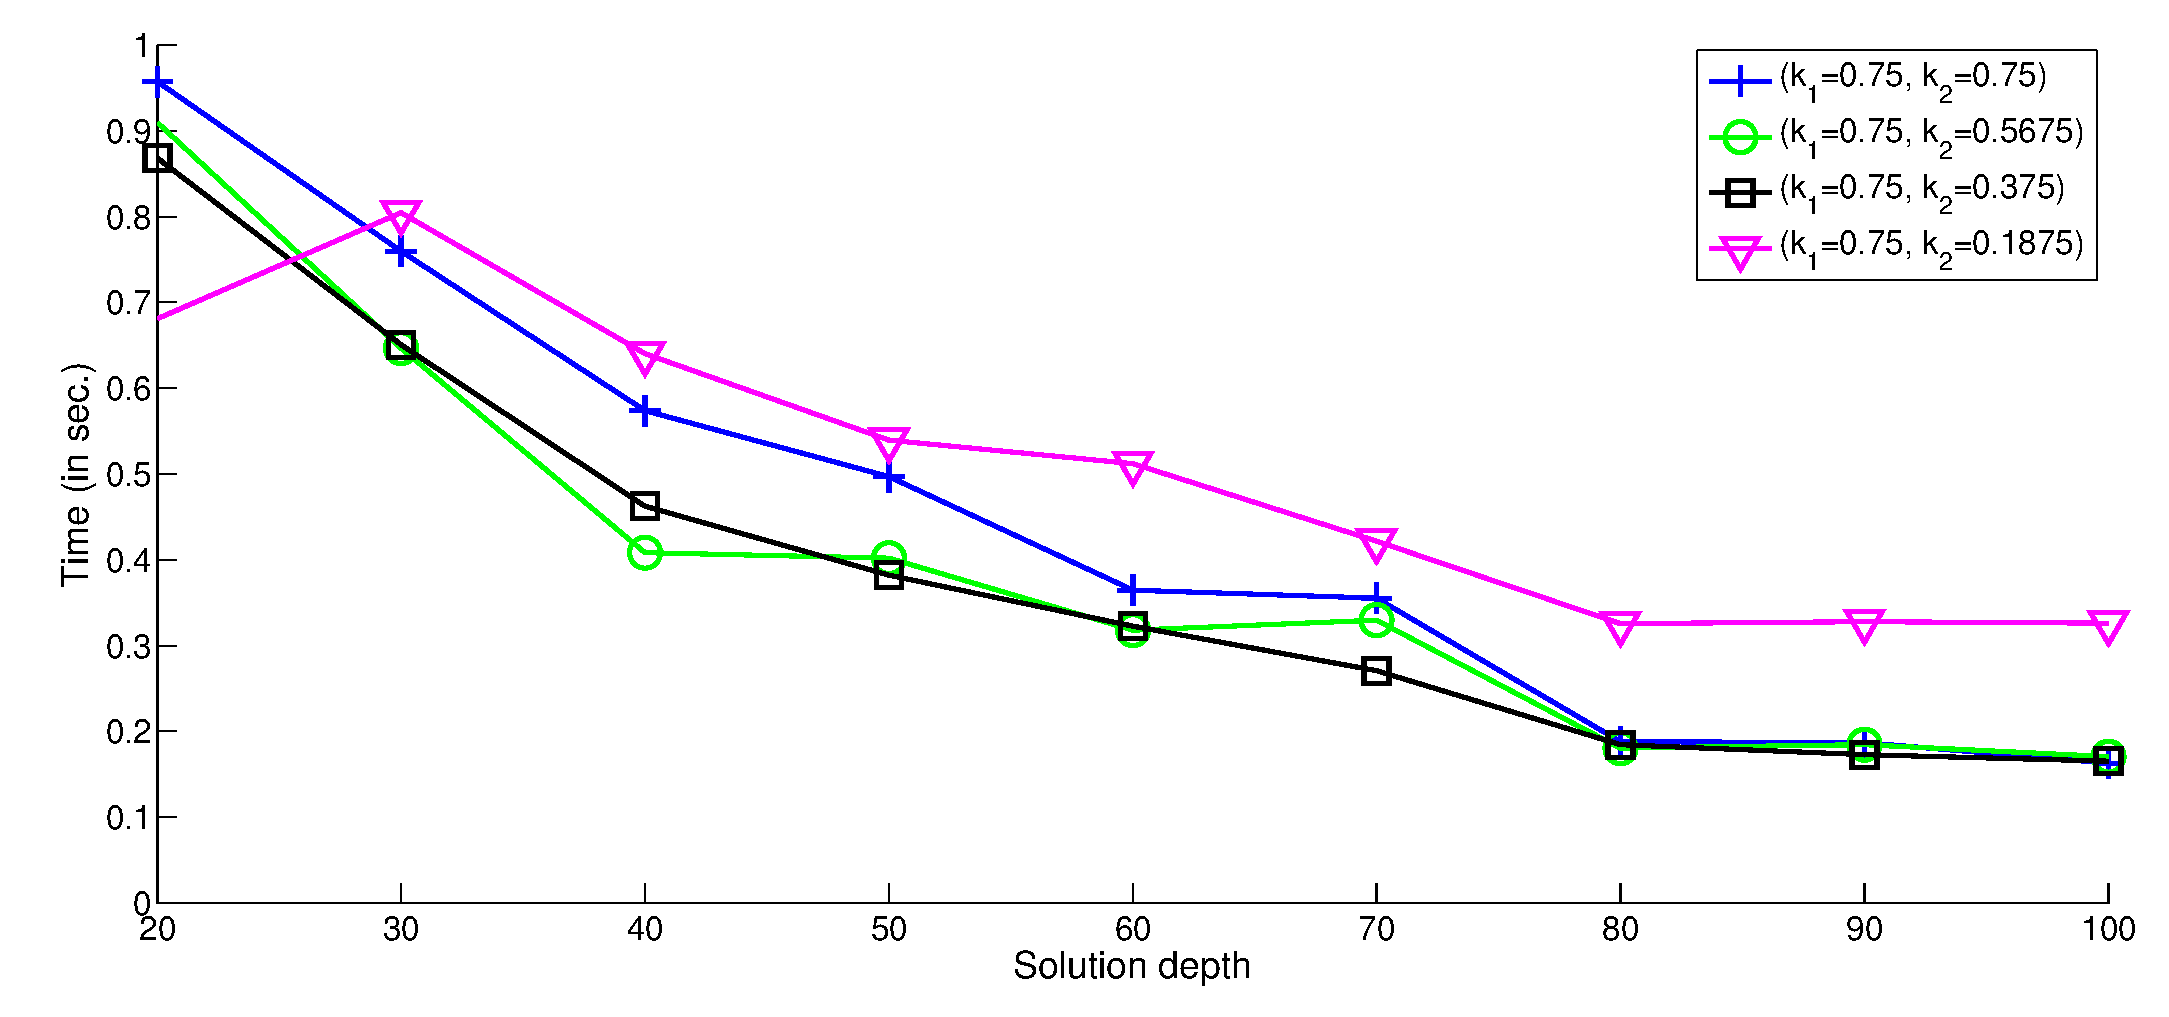
\includegraphics[width=0.95\textwidth]{Images/Chapter6/class2-exe-time-lexgo-te-a}
        }\\ %  ------- End of the first row ----------------------%
\vspace{0.025\textwidth}      
		\subfigure[$k_1 = 0.5$]{%
         \label{fig:6-13b}  
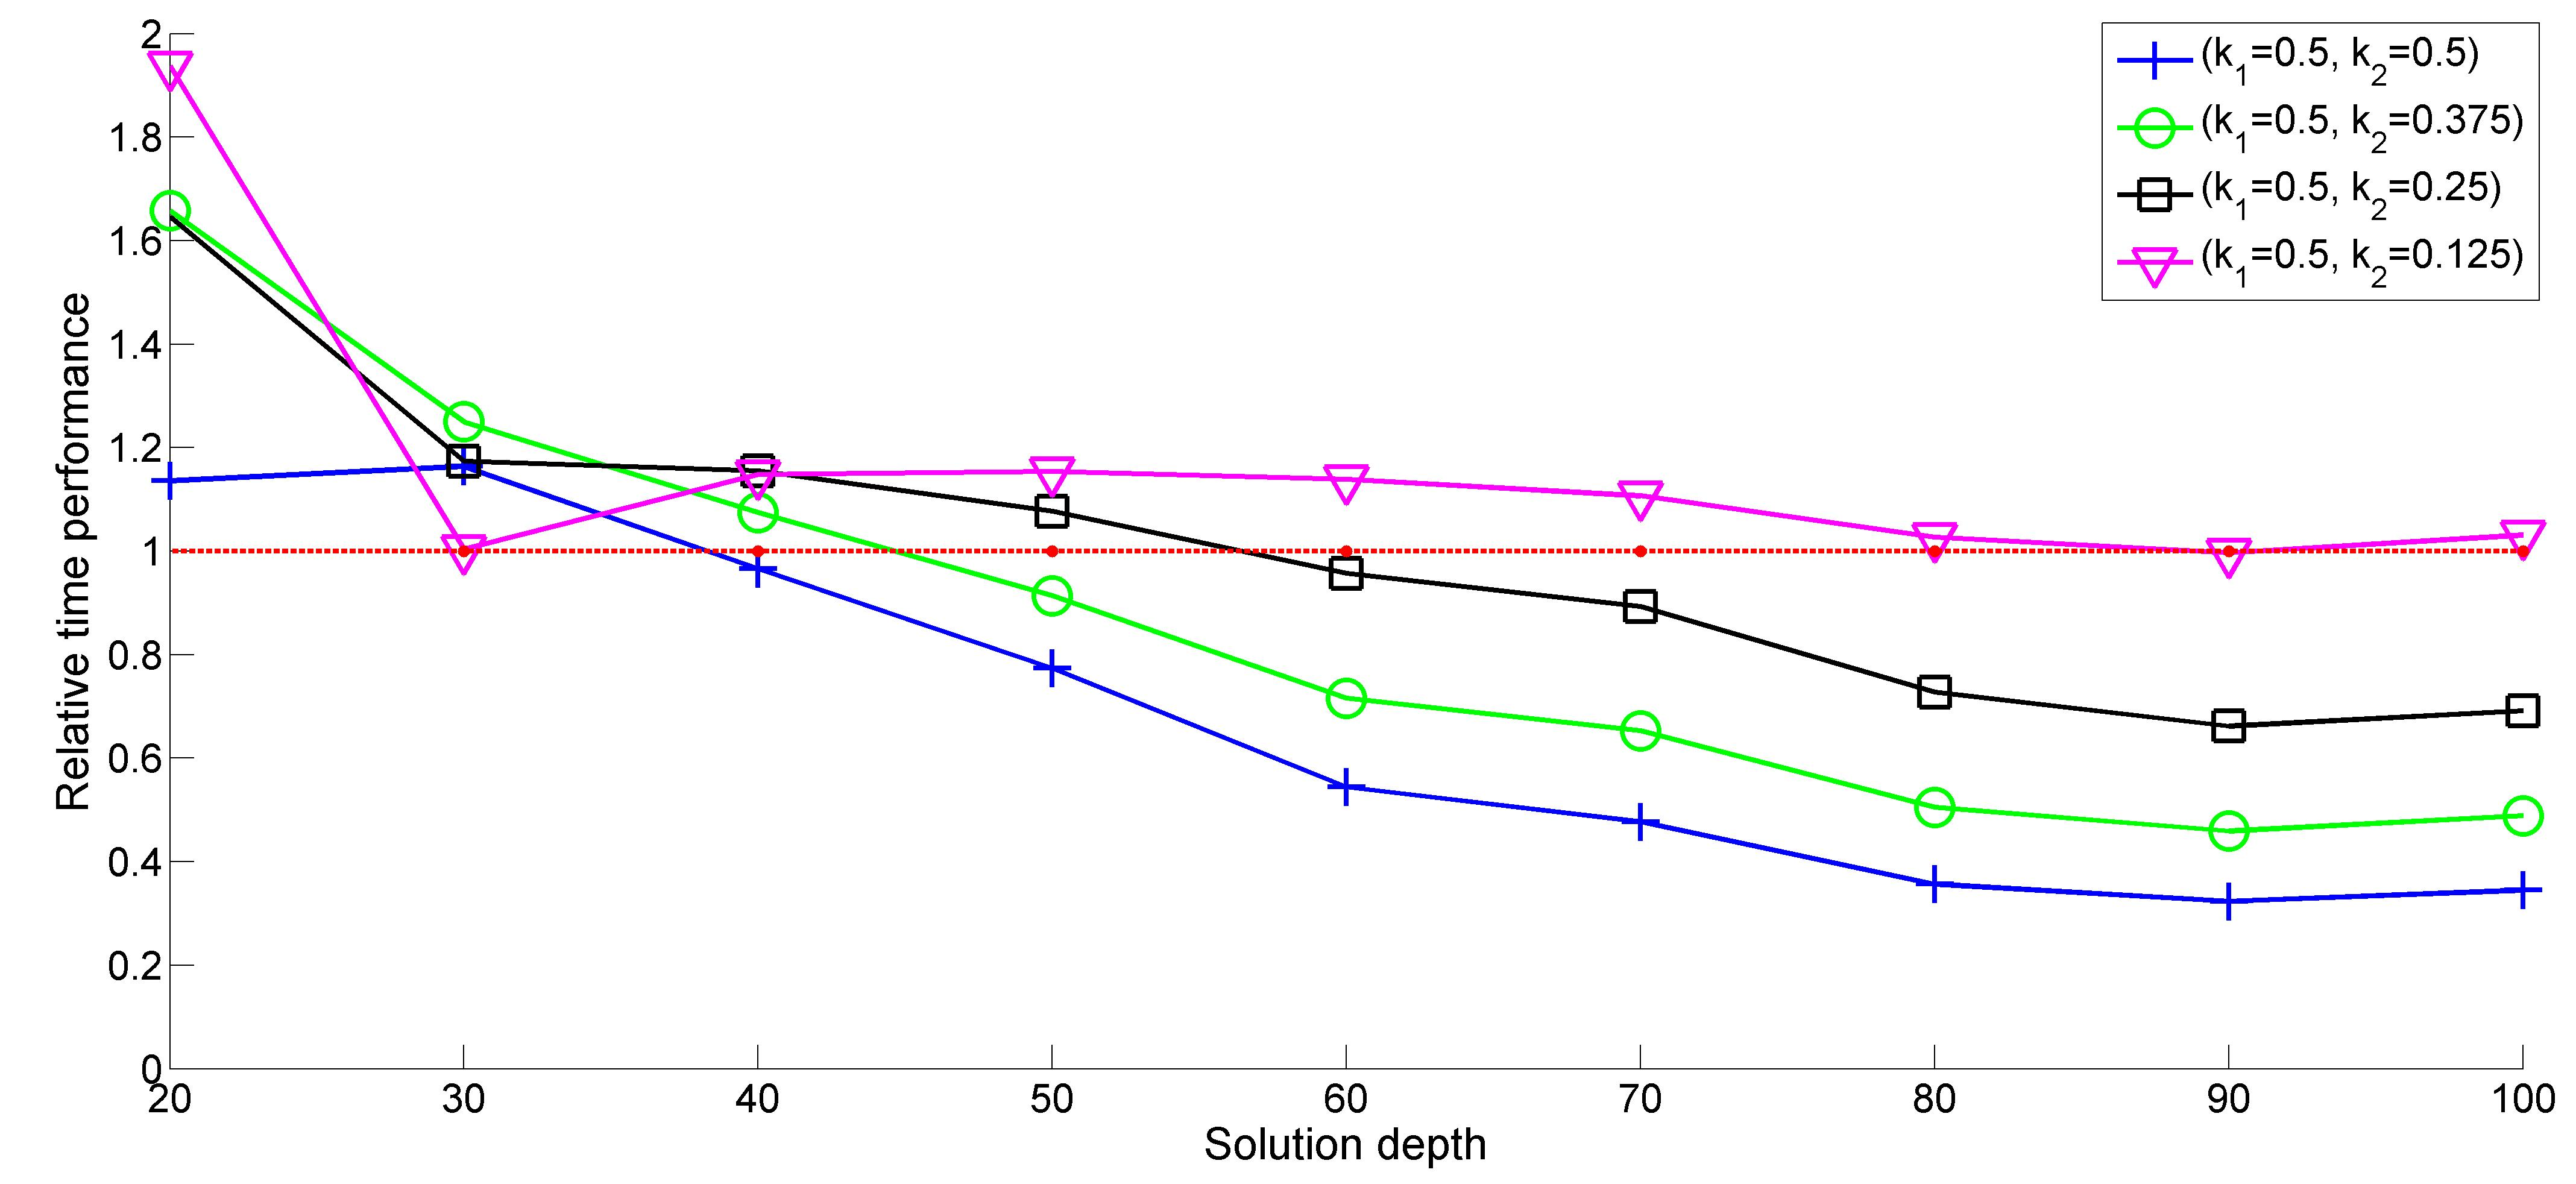
\includegraphics[width=0.95\textwidth]{Images/Chapter6/class2-exe-time-lexgo-te-b}
        }\\ %  ------- End of the first row ----------------------%
    \end{center}
    \vspace{-0.25in} 
    \caption{%
Class II experiments on grids, relative runtime performance (in seconds) of \lexgote \ over the best previous runtimes of \lexgo \ as a function of solution depth.
    }%
    \label{fig:6-13}
\end{figure}

%-------------------------------------------------------------------
\subsection{Summary}
\label{chapEmpiricalAnalysis:subsec:summarygridslexgote}
%-------------------------------------------------------------------

Just as in the case of \namoa, \lexgo \ can also be improved when applying the t-discarding method. This method can be applied to \lexgo \ when goals can be satisfied, i.e. when deviation vectors are $\vec 0$.

In a similar way as \namoate \ performs against \namoa \ (see Section \ref{chapEmpiricalAnalysis:sec:resultsgridsnamoate}), the speed-up of \lexgote \ over \lexgo \ grows with problem difficulty (see Figures \ref{fig:6-12},  and \ref{fig:6-13}), reducing time requirements over 88\% for the harder problems. In addition, \lexgote \ speed-up grows with the number of goal-optimal solution costs. Notice in Table \ref{tab:6-8} that \lexgote \ for $d=100$ runs 11\% faster with $k_1= 1$ than with $k_1=0.5$, despite of the fact that the number of label expansions is 40\% greater for $k_1=1$ than for $k_1=0.5$ (see Tables \ref{tab:6-2a} and \ref{tab:6-2b}). This is because the number of opportunities to apply t-discarding grows with the relative percentage of goal-optimal solution costs over the Pareto set. Hence, t-discarding is triggered on a more regular basis on these cases where $k_1$ is greater.

\lexgote \ does not show any improvement when goals cannot be satisfied, since the t-discarding can be barely applied to these problems. However, \lexgo \ achieves important reductions in time when goals can be satisfied, being three to eight times faster in class I experiments and up to six times faster in the second class of experiments.

%-------------------------------------------------------------------
\section{\texorpdfstring{\lexgote}{LEXGO*dr} \ vs \texorpdfstring{\namoate}{NAMOA*dr}}
\label{chapEmpiricalAnalysis:sec:resultsgridsfinal}
%-------------------------------------------------------------------

This section deals with the algorithms that employ the dimensionality reduction technique, \namoate \ and \lexgote. We have already seen the improvement of \namoate \ over \namoa, as well as \lexgote \ over \lexgo. In the following, a final time performance comparison between the two best alternatives is presented.

The experiments included in this section are applied to random grid problems with three objectives and goals described in Section \ref{chapEmpiricalAnalysis:sec:grids}.

%-------------------------------------------------------------------
\subsection{Analysis on class I experiments}
\label{chapEmpiricalAnalysis:subsec:analysisgridsfinalc1}
%-------------------------------------------------------------------

Table \ref{tab:6-10} shows the relative performance of \lexgote \ over \namoate \ for the solution depth equal to 100. \lexgote \ performs better than \namoate \ when goals cannot be satisfied, i.e. $k_1=\{0.25, 0\}$ but it is significantly slower when goals can be satisfied. It is also worth to pay attention to the relative performance when $k_1=1$ in comparison with $k_1=0.5$. The former performs around 40\% more label expansions (see Table \ref{tab:6-2}) and it is still faster than the latter. Notice that the number of scanned labels of both algorithms that employ the dimensionality reduction technique are equal to their versions without t-discarding, although the number of dominance checks is greatly reduced in \namoate \ and \lexgote.

Figure \ref{fig:6-14} displays the average runtimes of \namoate \ and \lexgote \ as a function of solution depth. The trend here is slightly in favor of \namoate \ over \lexgote \ for $k_1 \geq 0.5$.

\begin{table}
\caption{Class I experiments on grids, runtimes of \lexgote \ and \namoate \ for $d = 100$.}
\centering
\begin{tabular}{rrrrrr}
\hline \noalign{\smallskip}
 & \multicolumn{5}{c}{\lexgote} \\
\noalign{\smallskip} \cline{2-6} \noalign{\smallskip}
\namoate & $(k_1=1)$ & $(k_1=0.75)$ & $(k_1=0.5)$ & $(k_1=0.25)$ & $(k_1=0)$ \\
\noalign{\smallskip} 
Runtime (s) \\
\hline  \noalign{\smallskip} 
196.1 & 254.4 & 300.8 & 282.5 & 35.3 & 0.1 \\ 
%\hline
%\% & \% & \% & \% & \% & \% \\
%100\% & 129.7\% & 153.4\% & 144\% & 18\% & 0.04\% \\
\hline
\end{tabular}
\label{tab:6-10}
\end{table} 

\begin{figure}%[!ht]
\centering
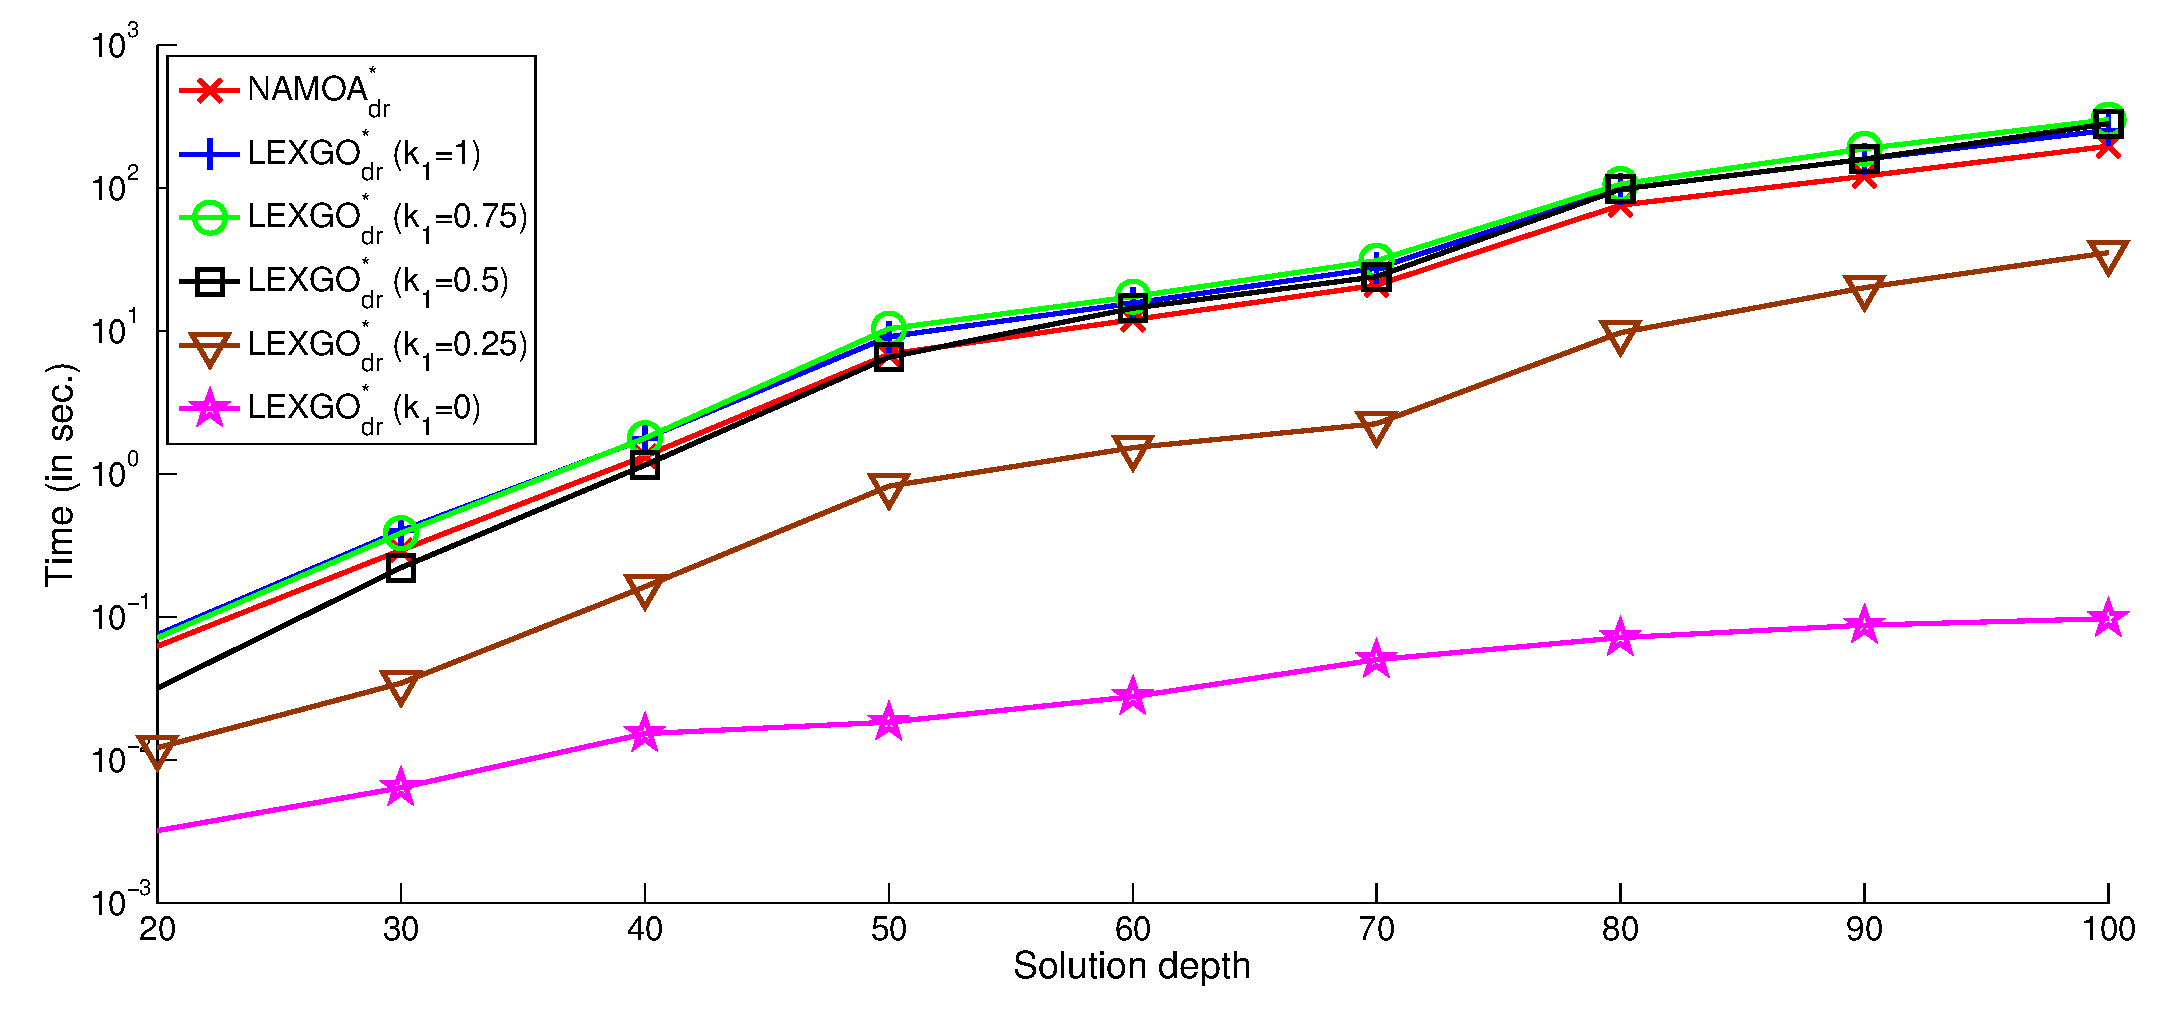
\includegraphics[width=1\textwidth]{Images/Chapter6/class1-exe-time-te}
\caption{Class I experiments on grids, average runtimes (in seconds) of \namoate \ and \lexgote \ per solution depth.}
\label{fig:6-14}
\end{figure}

%-------------------------------------------------------------------
\subsection{Analysis on class II experiments}
\label{chapEmpiricalAnalysis:subsec:analysisgridsfinalc2}
%-------------------------------------------------------------------

Regarding the second class of experiments, Table \ref{tab:6-11} shows \namoate \ and \lexgote \ runtimes for $k_1=0.75$ and $k_1=0.5$ with all $k_2$ possible values. Those cases where \lexgote \ outperforms \namoate \ are shown in bold. Figures \ref{fig:6-15a} and \ref{fig:6-15b} display the runtimes as a function of solution depth for $k_1=0.75$ and $k_1=0.5$, respectively. 

In these experiments, it can be observed that there are cases when goals are satisfiable and \lexgote \ is still faster than \namoate. On one hand, when $k_1=0.75, k_2=0.1875$ approximately 10\% of the Pareto frontier is returned (see Table \ref{tab:6-3}) and \lexgote \ is somewhat three times faster than \namoate. On the other hand, when $k_1=0.5$ and $k_2=0.25$ goals can also be satisfied and \lexgote \ outperforms \namoate. 

\begin{table}
\caption{Class II experiments on grids, \lexgote \ and \namoate \ runtimes (in seconds). Cases were \lexgote \ outperforms \namoate \ are highlighted in bold.}
\centering
\scalebox{0.9}{
\begin{tabular}{rrrrrrrrrrr}
\hline \noalign{\smallskip}
 &  & \multicolumn{8}{c}{\lexgote} & \\
\noalign{\smallskip} \cline{3-10}
 & \namoate & \multicolumn{4}{c|}{0.75} & \multicolumn{4}{c}{0.5} & \multicolumn{1}{c}{$k_1$}\\
$d$  & Runtime (s) & 0.75 & 0.5625 & 0.375 & \multicolumn{1}{c|}{0.1875} & 0.5 & 0.375 & 0.25 & 0.125 & \multicolumn{1}{c}{$k_2$}\\
\cline{1-10} \noalign{\smallskip} 
20 & 0.06 & 0.07 & \textbf{0.06} & \textbf{0.04} & \textbf{0.01} & \textbf{0.03} & \textbf{0.02} & \textbf{0.01} & \textbf{<0.01} \\ 
30 & 0.29 & 0.38 & 0.35 & \textbf{0.23} & \textbf{0.09} & \textbf{0.22} & \textbf{0.15} & \textbf{0.08} & \textbf{0.05} \\ 
40 & 1.3 & 1.7 & 1.6 & \textbf{1.1} & \textbf{0.38} & \textbf{1.1} & \textbf{0.81} & \textbf{0.42} & \textbf{0.24} \\ 
50 & 6.8 & 10.3 & 10.6 & \textbf{6.5} & \textbf{1.74} & \textbf{6.5} & \textbf{4.2} & \textbf{1.9} & \textbf{0.84} \\ 
60 & 11.9 & 17.3 & 19.3 & 13.5 & \textbf{3.6} & 14.4 & \textbf{10.4} & \textbf{4.8} & \textbf{1.8} \\  
70 & 20.9 & 30.8 & 32.2 & 22.8 & \textbf{6.8} & 24.0 & \textbf{17.7} & \textbf{8.5} & \textbf{2.9} \\
80 & 76.0 & 105.9 & 133.1 & 95.0 & \textbf{24.0} & 97.8 & \textbf{68.5} & \textbf{29.4} & \textbf{17.4} \\ 
90 & 120.6 & 187.9 & 219.8 & 156.5 & \textbf{41.2} & 158.7 & \textbf{117.8} & \textbf{53.3} & \textbf{40.0} \\ 
100 & 196.1 & 300.8 & 389.6 & 283.7 & \textbf{63.4} & 282.4 & 199.1 & \textbf{84.7} & \textbf{82.1} \\ 
\hline
\end{tabular}
}
\label{tab:6-11}
\end{table} 

\begin{figure}
    \begin{center}
%
      \subfigure[$k_1 = 0.75$]{%
         \label{fig:6-15a}
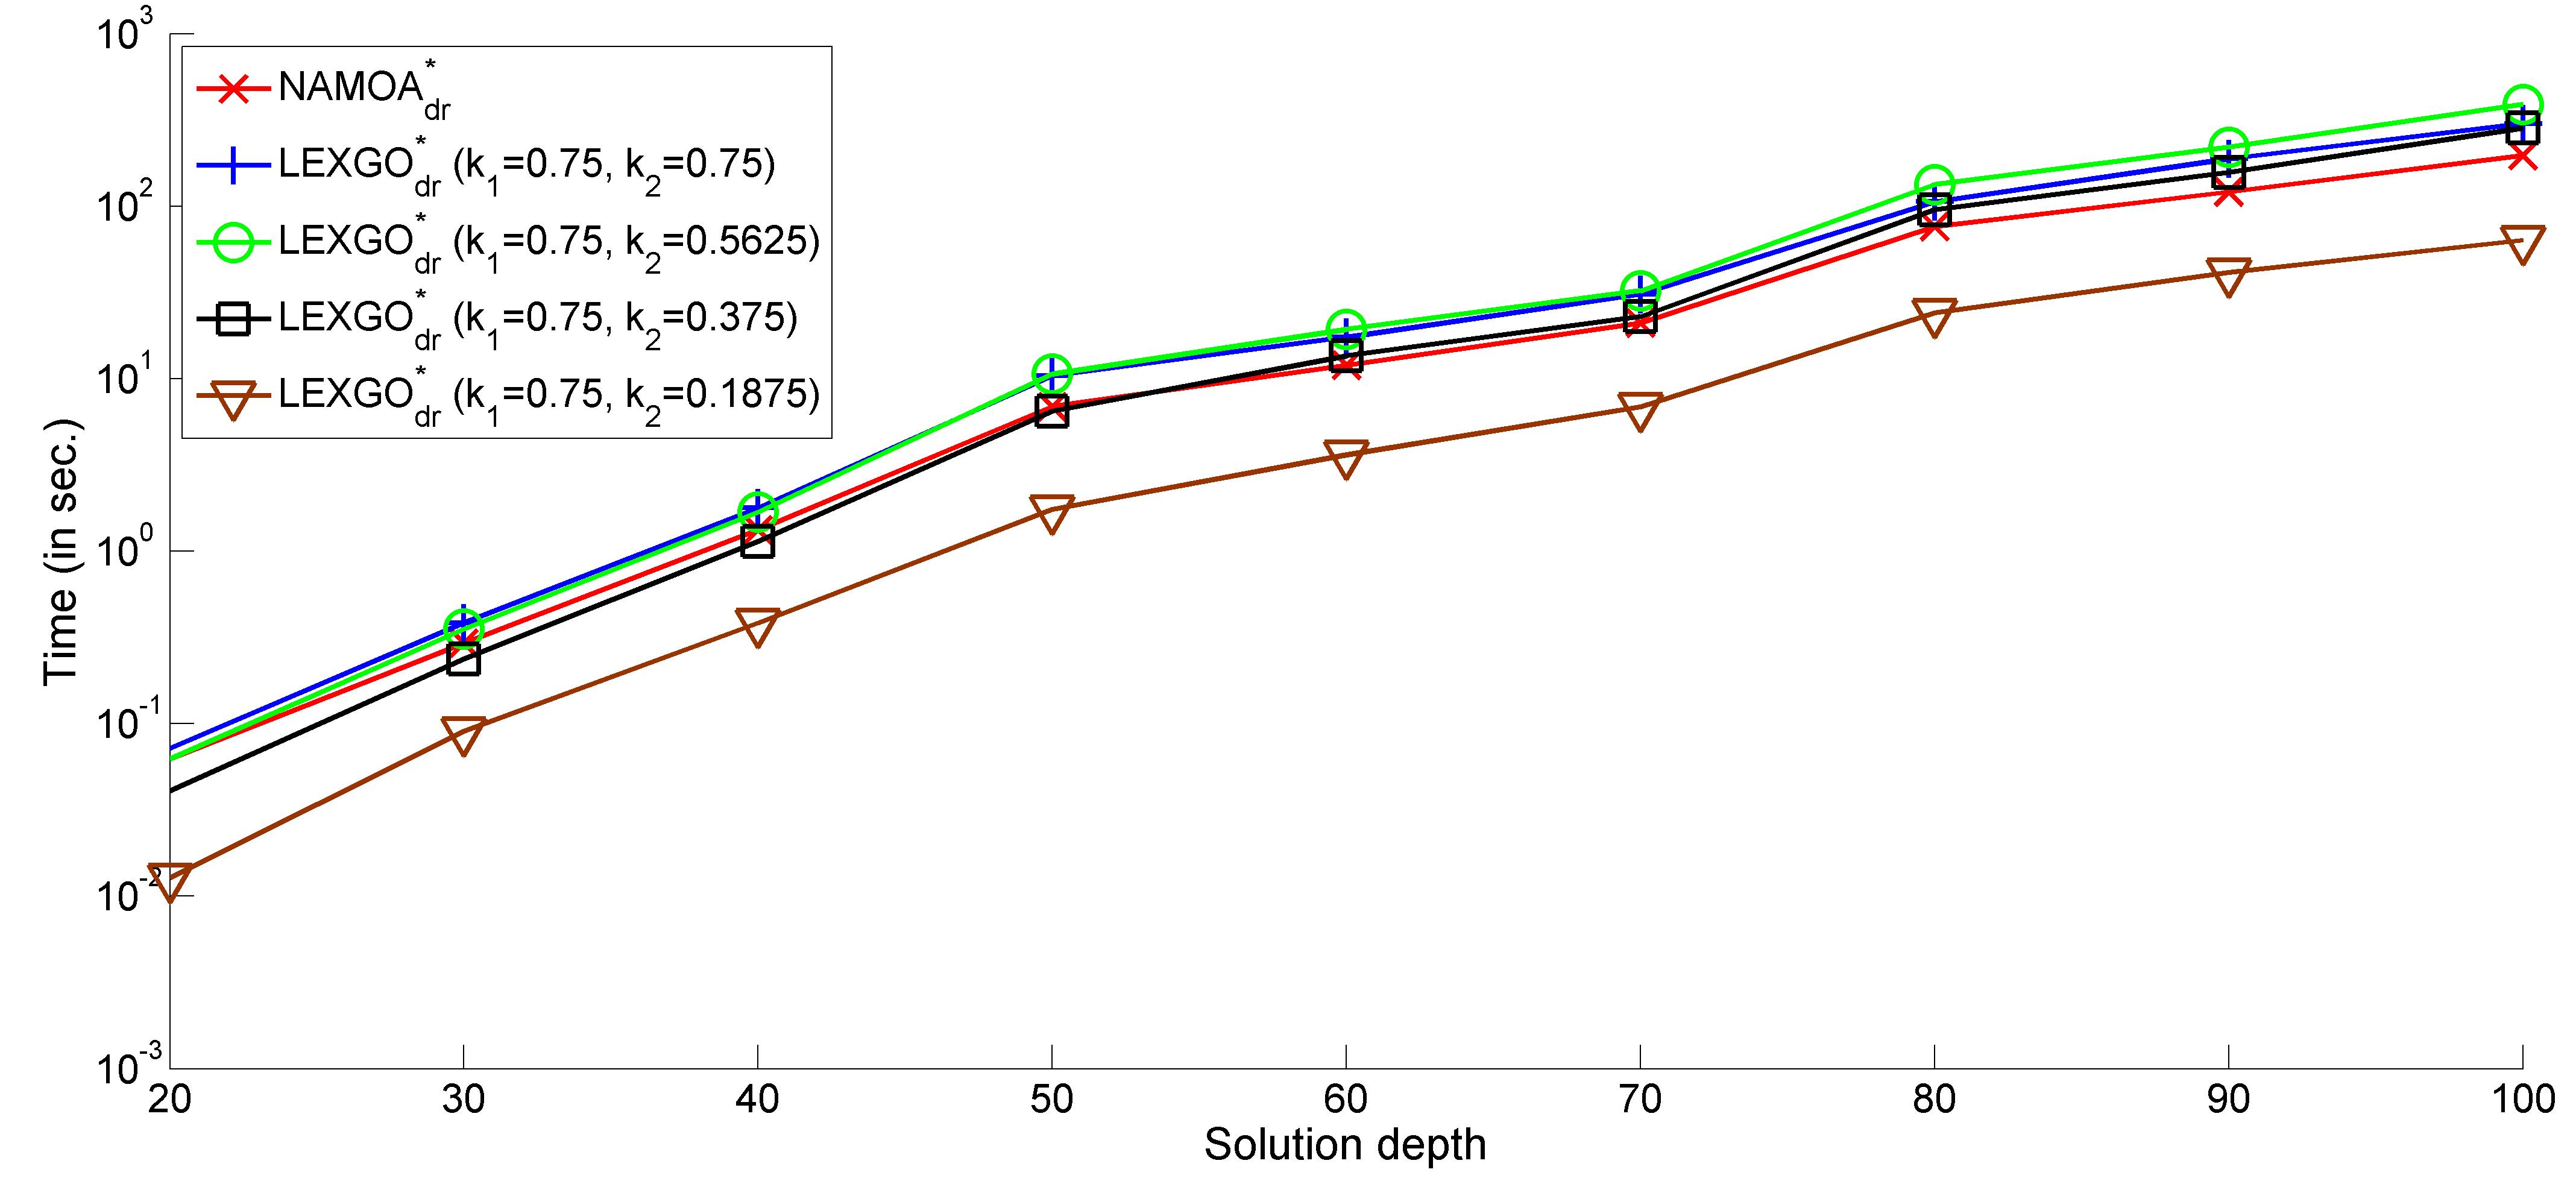
\includegraphics[width=0.95\textwidth]{Images/Chapter6/class2-exe-time-te-a}
        }\\ %  ------- End of the first row ----------------------%
\vspace{0.025\textwidth}      
		\subfigure[$k_1 = 0.5$]{%
         \label{fig:6-15b}  
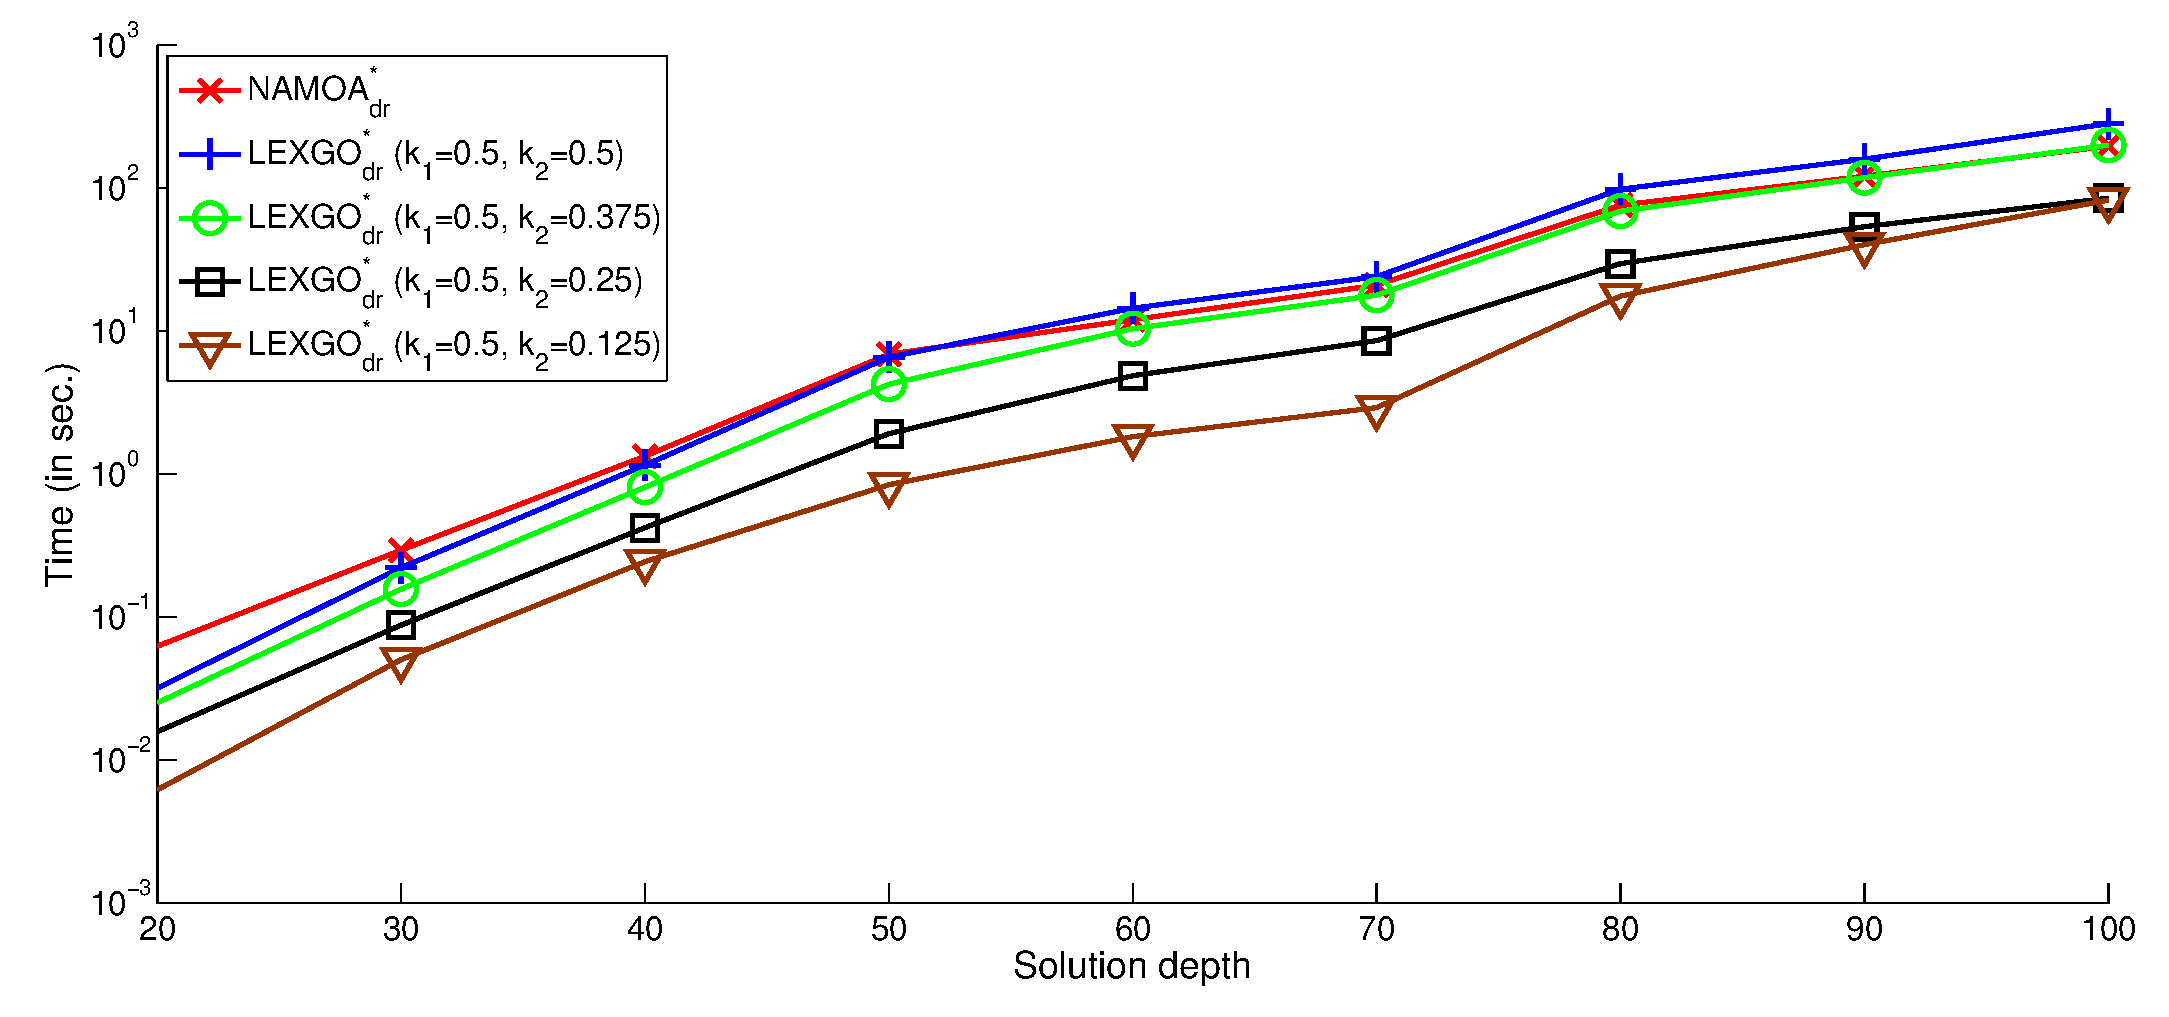
\includegraphics[width=0.95\textwidth]{Images/Chapter6/class2-exe-time-te-b}
        }\\ %  ------- End of the first row ----------------------%
    \end{center}
    \vspace{-0.25in} 
    \caption{%
Class II experiments on grids, average runtimes in seconds of \lexgote \ and \namoate \ per solution depth.
    }%
    \label{fig:6-15}
\end{figure}

%-------------------------------------------------------------------
\subsection{Summary}
\label{chapEmpiricalAnalysis:subsec:summarygridste}
%-------------------------------------------------------------------

The experimental comparison between \namoate \ and \lexgote \ is one of the contributions of this thesis. On one hand, \lexgote \ is the application of the successful technique of t-discarding dominated paths to the algorithm \lexgo, which has also been proposed in this thesis. In fact, these results are new to the literature and expose a significant different behavior than the comparison between \lexgo \ and \namoa \ showed in Section \ref{chapEmpiricalAnalysis:sec:resultsgridslexgo}. Despite \lexgo \ has been proved to be more efficient than \namoa \ (see Section \ref{chapFormalAnalysis:sec:efficiencyLexgo}), the same cannot be asserted when the t-discarding technique is applied to both algorithms. 

Both \namoate \ and \lexgote \ achieve a speed-up of about an order of magnitude for our random grid problem experiments over \namoa \ and \lexgo, respectively. However, \lexgote \ cannot apply the t-discarding method when a path does not satisfy goals and therefore, the applicability of this technique is partial, even though practically is applied to an average of 99.5\% of the pruning operations. This small percentage of iterations that must perform the classical dominance checks clearly affect the runtime performance of \lexgote \ in comparison with \namoate. Thus, \namoate \ becomes the option to be selected when goals can be satisfied while \lexgote \ is still preferred when goals cannot be satisfied and the path which minimizes the deviation from goals has to be returned.      

%-------------------------------------------------------------------
\section{Summary on random grid experiments}
\label{chapEmpiricalAnalysis:sec:summarygridsfinal}
%-------------------------------------------------------------------

Previous results to the experiments showed in this thesis were reported in \citet{Pulido2014} and \citet{Pulido2015}. The experiments reported in this chapter go beyond those previously reported and add \lexgolin \ and \lexgote \ algorithms to the analyses. Furthermore, additional cases of \lexgo \ have been evaluated, for instance, $k_1=0.75$ in class II experiments. 

A summary of the runtime performance obtained from the evaluation of the algorithms \namoalex, \namoalin, \lexgolex, \lexgolin, \namoate \ and \lexgote \
is presented in Table \ref{tab:6-12}. A detailed analysis for class I and II experiments follows. 

\begin{table}
\caption{Runtime comparison - summary table for random grid experiments.}
\centering
\scalebox{0.92}{
\begin{tabular}{p{0.35\textwidth}p{0.65\textwidth}}
\hline \noalign{\smallskip}
\textbf{Comparison} & Results \\
\noalign{\smallskip} \hline
%& Class I & Class II \\
\noalign{\smallskip}
\textbf{\namoalin \ vs \namoalex} & \namoalin \ outperforms \namoalex \ by a factor of two in all cases. Its comparative advantage slightly grows with problem difficulty. \\
\noalign{\smallskip}\hline
\noalign{\smallskip}
\textbf{\lexgolin \ vs \lexgolex} & \lexgolin \ outperforms \lexgolex \ by a factor of 1.8 when a high percentage of the non-dominated cost vectors satisfy the goals. When this percentage is smaller \lexgolex \ outperforms \lexgolin. Both have similar performance when goals cannot be satisfied. \\
\noalign{\smallskip}\hline
\noalign{\smallskip}
\textbf{\lexgo \ vs \namoa} & The lexicographic order is comparatively more advantageous in runtime for \lexgo \ than the linear. With both selection orders, \lexgo \ runs faster than \namoa \ for $k_1 = 0.5$, around two orders of magnitude faster when $k_1 = 0.25$, and several orders of magnitude faster for $k_1 = 0$. A small time overhead can be observed for \lexgo \ with $k_1 = 1$ and in some cases with $k_1 = 0.75$. \\
\noalign{\smallskip}\hline
\noalign{\smallskip}
\textbf{\namoate \ vs \namoa} & \namoate \ is consistently faster than \namoalex \ and \namoalin. Its advantage in runtime clearly grows with problem difficulty. \\
\noalign{\smallskip}\hline
\noalign{\smallskip}
\textbf{\lexgote \ vs \lexgo} & Their performance is similar when goals cannot be satisfied. However, \lexgote \ achieves important reductions in runtime when goals can be satisfied. \lexgote \ runtime advantage grows with the number of goal-optimal solution costs and with problem difficulty. \\
\noalign{\smallskip}\hline
\noalign{\smallskip}
\textbf{\lexgote \ vs \namoate} & \lexgote \ is faster than \namoate \ when goals cannot be satisfied. \namoate \ performs faster when goals can be satisfied. \\
%Surprisingly, \lexgote \ has a comparatively worse performance against \namoate \ when a portion of the Pareto frontier satisfies the goals, and performs better when all non-dominated solutions satisfy the goals. \\
\hline
\end{tabular}
}
\label{tab:6-12}
\end{table}

%-------------------------------------------------------------------
\subsection{Summary on class I experiments}
\label{chapEmpiricalAnalysis:subsec:summarygridsfinalc1}
%-------------------------------------------------------------------

Table \ref{tab:6-13} shows all runtimes for class I experiments and all algorithms evaluated. \namoate \ runtimes and those experiments of \lexgo \ which perform faster than \namoate \ are highlighted in bold. Thus, the empirical evaluation of all considered alternatives draws a clear picture on the performance of each algorithm, resulting generally in \namoate \ as the best algorithm when goals can be satisfied and \lexgote \ when goals cannot be satisfied. Moreover, the t-discarding technique improves over an order of magnitude both algorithms \namoate \ and \lexgote \ over \namoa \ and \lexgo, and does not affect significantly the runtime of \lexgo \ when goals cannot be satisfied. 

\begin{table}
\caption{Class I experiments on grids, runtimes (in seconds) of all algorithms studied in this thesis as a function of solution depth.}
\centering
\scalebox{0.86}{
\begin{tabular}{lrrrrrrrrr}
\hline \noalign{\smallskip} 
Depth & {20} & {30} & {40} & {50} & {60} & {70} & {80} & {90} & {100}\\
\noalign{\smallskip} \hline
\namoalex & 0.06 & 0.47 & 3.53 & 36.83 & 86.94 & 178.53 & 1,164.12 & 2,030.07 & 3,662.93 \\
\noalign{\smallskip}
\namoalin & 0.06 & 0.37 & 2.36 & 18.37 & 43.84 & 83.38 & 533.80 & 981.32 & 1,754.44 \\
\noalign{\smallskip}
\namoate & \textbf{0.06} & \textbf{0.29} & \textbf{1.33} & \textbf{6.87} & \textbf{11.95} & \textbf{20.94} & \textbf{76.01} & \textbf{120.67} & \textbf{196.14} \\
\noalign{\smallskip}
\lexgolex & \multicolumn{9}{l} \space  \\
$(k_1=1)$  & 0.07 & 0.52 & 3.70 & 37.35 & 88.89 & 179.67 & 1,202.71 & 2,115.23 & 3,763.78 \\ 
$(k_1=0.75)$  & 0.07 & 0.46 & 3.23 & 31.20 & 78.87 & 157.80 & 1,074.36 & 1,781.12 & 3,381.33 \\
$(k_1=0.5)$  & \textbf{0.03} & \textbf{0.19} & \textbf{1.20} & 8.44 & 26.54 & 50.37 & 274.42 & 490.95 & 819.28 \\
$(k_1=0.25)$  & \textbf{0.01} & \textbf{0.03} & \textbf{0.14} & \textbf{0.74} & \textbf{1.36} & \textbf{2.02} & \textbf{9.34} & \textbf{19.55} & \textbf{33.47} \\
$(k_1=0)$  & \textbf{<0.01} & \textbf{<0.01} & \textbf{0.01} & \textbf{0.02} & \textbf{0.02} & \textbf{0.03} & \textbf{0.05} & \textbf{0.07} & \textbf{0.07} \\
\noalign{\smallskip}
\lexgolin & \multicolumn{9}{l} \space  \\
$(k_1=1)$  & 0.09 & 0.52 & 3.10 & 21.18 & 48.77 & 95.36 & 606.91 & 1,141.97 & 2,114.18 \\ 
$(k_1=0.75)$  & 0.07 & 0.51 & 3.10 & 20.88 & 47.68 & 87.01 & 563.05 & 1,006.66 & 1,847.88 \\
$(k_1=0.5)$  & \textbf{0.03} & \textbf{0.31} & 2.36 & 14.55 & 39.54 & 60.51 & 387.28 & 620.69 & 1,145.15 \\
$(k_1=0.25)$  & \textbf{0.01} & \textbf{0.03} & \textbf{0.18} & \textbf{0.92} & \textbf{1.70} & \textbf{2.55} & \textbf{11.04} & \textbf{21.58} & \textbf{37.45} \\
$(k_1=0)$  & \textbf{<0.01} & \textbf{0.01} & \textbf{0.01} & \textbf{0.02} & \textbf{0.02} & \textbf{0.04} & \textbf{0.07} & \textbf{0.09} & \textbf{0.09} \\
\noalign{\smallskip}
\lexgote & \multicolumn{9}{l} \space  \\
$(k_1=1)$  & 0.08 & 0.40 & 1.77 & 9.08 & 15.69 & 27.46 & 98.24 & 158.32 & 254.40 \\ 
$(k_1=0.75)$  & 0.07 & 0.38 & 1.78 & 10.38 & 17.38 & 30.89 & 105.95 & 187.93 & 300.86 \\
$(k_1=0.5)$  & \textbf{0.03} & \textbf{0.22} & \textbf{1.15} & \textbf{6.53} & 14.44 & 24.03 & 97.85 & 158.71 & 282.49 \\
$(k_1=0.25)$  & \textbf{0.01} & \textbf{0.03} & \textbf{0.16} & \textbf{0.82} & \textbf{1.53} & \textbf{2.25} & \textbf{9.76} & \textbf{20.03} & \textbf{35.37} \\
$(k_1=0)$  & \textbf{<0.01} & \textbf{0.01} & \textbf{0.02} & \textbf{0.02} & \textbf{0.03} & \textbf{0.05} & \textbf{0.07} & \textbf{0.09} & \textbf{0.10} \\
\hline
\end{tabular}
}
\label{tab:6-13}
\end{table}

%-------------------------------------------------------------------
\subsection{Summary on class II experiments}
\label{chapEmpiricalAnalysis:subsec:summarygridsfinalc2}
%-------------------------------------------------------------------

With respect to class II experiments, Table \ref{tab:6-14} shows all runtimes for class II experiments and all algorithms evaluated. \namoate \ runtimes and those experiments of \lexgo \ which perform faster than \namoate \ are also highlighted in bold. 

There are eight different cases for each solution depth with the combinations of $k_1 = \{0.75, 0.5 \}$ and $k_2$ calculated as described in Equation \ref{eq:targets2}. It can be observed that the number of cases where \lexgote \ outperforms \namoate \ decreases with solution depth. For instance, the number of cases where \lexgote \ is faster than \namoate \ decreases from 7 out of 8 when $d = 20$ to 3 out of 8 when $d = 100$. It is expected that \namoate \ will  outperform \lexgote \ in runtime performance in more difficult problems. 

\begin{table}
\caption{Class II experiments on grids, runtimes (in seconds) of all algorithms studied in this thesis as a function of solution depth.}
\centering
\scalebox{0.86}{
\begin{tabular}{lrrrrrrrrr}
\hline \noalign{\smallskip} 
Depth & {20} & {30} & {40} & {50} & {60} & {70} & {80} & {90} & {100}\\
\noalign{\smallskip} \hline
\namoalex & 0.06 & 0.47 & 3.53 & 36.83 & 86.94 & 178.53 & 1,164.12 & 2,030.07 & 3,662.93 \\
\noalign{\smallskip}
\namoalin & 0.06 & 0.37 & 2.36 & 18.37 & 43.84 & 83.38 & 533.80 & 981.32 & 1,754.44 \\
\noalign{\smallskip}
\namoate & \textbf{0.06} & \textbf{0.29} & \textbf{1.33} & \textbf{6.87} & \textbf{11.95} & \textbf{20.94} & \textbf{76.01} & \textbf{120.67} & \textbf{196.14} \\
\noalign{\smallskip}
\lexgolex & \multicolumn{9}{l} \space  \\
$(0.75, \ 0.75)$  & 0.07 & 0.46 & 3.23 & 31.20 & 78.87 & 157.80 & 1,074.36 & 1,781.12 & 3,381.33 \\
$(0.75, \ 0.5625)$ &  \textbf{0.04} & 0.39 & 2.47 & 22.14 & 58.66 & 120.67 & 809.09 & 1,401.87 & 2,444.38 \\
$(0.75, \ 0.375)$  & \textbf{0.03} & \textbf{0.22} & \textbf{1.25} & 9.56 & 25.65 & 55.71 & 324.66 & 639.08 & 1,013.19 \\
$(0.75, \ 0.1875)$  & \textbf{0.01} & \textbf{0.08} & \textbf{0.34} & \textbf{1.76} & \textbf{3.98} & \textbf{8.95} & \textbf{39.93} & \textbf{76.38} & \textbf{108.27} \\
\noalign{\smallskip}
$(0.5, \ 0.5)$  & \textbf{0.03} & \textbf{0.19} & \textbf{1.20} & 8.44 & 26.54 & 50.37 & 274.42 & 490.95 & 819.28 \\
$(0.5, \ 0.375)$  & \textbf{0.02} & \textbf{0.12} & \textbf{0.75} & \textbf{4.64} & 14.51 & 27.16 & 135.74 & 256.56 & 407.47 \\
$(0.5, \ 0.25)$  & \textbf{0.01} & \textbf{0.07} & \textbf{0.37} & \textbf{1.78} & \textbf{5.07} & \textbf{9.58} & \textbf{40.52} & \textbf{80.67} & \textbf{122.57} \\
$(0.5, \ 0.125)$  & \textbf{<0.01} & \textbf{0.05} & \textbf{0.21} & \textbf{0.73} & \textbf{1.59} & \textbf{2.63} & \textbf{16.99} & \textbf{40.18} & \textbf{79.69} \\
\noalign{\smallskip}
\lexgolin & \multicolumn{9}{l} \space  \\
$(0.75, \ 0.75)$  & 0.07 & 0.51 & 3.10 & 20.88 & 47.68 & 87.01 & 563.05 & 1,006.66 & 1,847.88 \\
$(0.75, \ 0.5625)$ &  0.07 & 0.55 & 4.12 & 26.45 & 60.75 & 97.91 & 738.42 & 1,191.72 & 2,285.11 \\
$(0.75, \ 0.375)$  & \textbf{0.05} & 0.37 & 2.46 & 16.99 & 41.98 & 84.46 & 514.54 & 906.98 & 1,719.23 \\
$(0.75, \ 0.1875)$  & \textbf{0.02} & \textbf{0.11} & \textbf{0.60} & \textbf{3.24} & \textbf{7.07} & \textbf{16.25} & \textbf{73.87} & 125.71 & 194.55 \\
\noalign{\smallskip}
$(0.5, \ 0.5)$  & \textbf{0.03} & 0.31 & 2.36 & 14.55 & 39.54 & 60.51 & 387.28 & 620.69 & 1,145.15 \\
$(0.5, \ 0.375)$  & \textbf{0.02} & \textbf{0.21} & 1.48 & 9.26 & 27.15 & 47.45 & 264.65 & 473.42 & 809.28 \\
$(0.5, \ 0.25)$  & \textbf{0.02} & \textbf{0.10} & \textbf{0.62} & \textbf{3.33} & \textbf{9.89} & \textbf{17.70} & 78.02 & 152.09 & 229.97 \\
$(0.5, \ 0.125)$  & \textbf{0.01} & \textbf{0.06} & \textbf{0.27} & \textbf{0.97} & \textbf{2.12} & \textbf{3.51} & \textbf{21.35} & \textbf{46.80} & \textbf{92.27} \\
\noalign{\smallskip}
\lexgote & \multicolumn{9}{l} \space  \\
$(0.75, \ 0.75)$  & 0.07 & 0.38 & 1.78 & 10.38 & 17.38 & 30.89 & 105.95 & 187.93 & 300.86 \\
$(0.75, \ 0.5625)$ &  \textbf{0.06} & 0.35 & 1.68 & 10.62 & 19.30 & 32.24 & 133.15 & 219.81 & 389.68 \\
$(0.75, \ 0.375)$  & \textbf{0.04} & \textbf{0.24} & \textbf{1.14} & \textbf{6.49} & 13.53 & 22.85 & 95.03 & 156.58 & 283.77 \\
$(0.75, \ 0.1875)$  & \textbf{0.01} & \textbf{0.09} & \textbf{0.38} & \textbf{1.75} & \textbf{3.62} & \textbf{6.85} & \textbf{24.03} & \textbf{41.21} & \textbf{63.41} \\
\noalign{\smallskip}
$(0.5, \ 0.5)$ & \textbf{0.03} & \textbf{0.22} & \textbf{1.15} & \textbf{6.53} & 14.44 & 24.03 & 97.85 & 158.71 & 282.49 \\
$(0.5, \ 0.375)$ & \textbf{0.03} & \textbf{0.16} & \textbf{0.81} & \textbf{4.24} & \textbf{10.39} & \textbf{17.73} & \textbf{68.58} & \textbf{117.82} & 199.12 \\
$(0.5, \ 0.25)$ & \textbf{0.02} & \textbf{0.09} & \textbf{0.42} & \textbf{1.92} & \textbf{4.85} & \textbf{8.55} & \textbf{29.48} & \textbf{53.39} & \textbf{84.79} \\
$(0.5, \ 0.125)$ & \textbf{0.01} & \textbf{0.05} & \textbf{0.24} & \textbf{0.84} & \textbf{1.82} & \textbf{2.91} & \textbf{17.45} & \textbf{40.04} & \textbf{82.18} \\
\hline
\end{tabular}
}
\label{tab:6-14}
\end{table}


%---------------------------------------------------------------------
%
% Chapter 7: Empirical Analysis On Road Map Problems
%
%---------------------------------------------------------------------
%
% ChapEmpiricalAnalysisRoadMaps.tex
% Copyright 2015 Dr. Francisco J. Pulido
%
% This file belongs to the PhD titled "New Techniques and Algorithms for Multiobjective and Lexicographic Goal-Based Shortest Path Problems", distributed under the Creative Commons Licence Attribution-NonCommercial-NoDerivs 3.0, available in http://creativecommons.org/licenses/by-nc-nd/3.0/. The complete PhD dissertation is freely accessible from http://www.lcc.uma.es/~francis/
%
% This thesis has been written adapting the TeXiS template, a LaTeX template for writting thesis and other documents. The complete TeXiS package can be obtained from http://gaia.fdi.ucm.es/projects/texis/. TeXis is distributed under the same conditions of the LaTeX Project Public License (http://www.latex-project.org/lppl.txt). The complete license is available in http://creativecommons.org/licenses/by-sa/3.0/legalcode
%
%---------------------------------------------------------------------

\chapter{Empirical Analysis On Road Map Problems}
\label{chapEmpiricalAnalysisRoadMaps}
%
\begin{FraseCelebre}
\begin{Frase}
The rise of Google, the rise of Facebook, the rise of Apple, I think are proof that there is a place for computer science as something that solves problems that people face every day.
\end{Frase}
\begin{Fuente}
Eric Schmidt (1955-)
\end{Fuente}
\end{FraseCelebre}
%
%\begin{resumen}
%

This chapter is devoted to analyze the algorithmic performance on realistic road maps from the "9th DIMACS Implementation Challenge: Shortest Path". The challenge comprises a set of twelve road maps of increasing size. In particular, we use the New York city map. Additionally we have employed a second road map from the UA Census 2000 TIGER/Line Files, which was assembled by Dr. Dominik Schultes\footnote{<mail@dominik-schultes.de>} and is available from the same site. In particular, we use the Vermont State map.

All DIMACS maps provide two different cost values: \textit{physical distance} and \textit{travel time}. An additional cost was introduced in \cite{Machuca2011} by calculating the \textit{travel economic cost}. This was obtained combining tolls and fuel consumption according to road category. The resulting values are not linearly correlated to those of the other cost values. The experiments reported below consider the simultaneous minimization of these three attributes, physical distance $(c_1)$, travel time $(c_2)$, and travel economic cost $(c_3)$ (further details about these experiments can be seen in  Section \ref{chapMultiObjTestBeds:subsec:RoadMaps}). 

The two maps selected for our experiments have different sizes. Table \ref{tab:7-1} shows the coordinates and number of nodes and arcs for each map. The NY city map represents a difficult problem to be tackled with three objectives and only some problems could be solved. The other map, VT$_{cut}$, corresponds to a trimmed version of the original map of Vermont, reduced to approximately 70\% of its original size in order to allow the solution of the complete set of experiments by all the algorithms. Renderings of the NY and VT$_{cut}$ maps are presented in Figures \ref{fig:7-1} and \ref{fig:7-2}, respectively.

\begin{table}
\caption{Maps employed in the road map experiments. ($^*$) corresponds to a cut of the original map.}
\label{tab:7-1}
\begin{center}
\begin{tabular}{ccrrrr}
\hline \noalign{\smallskip} 
Description & Acronym & Nodes & Arcs & Longitude & Latitude \\
\noalign{\smallskip} \hline 
New York city& NY & 264,346 & 730,100 & [73.5-74.5]$^{\circ}$W & [40.3-41.3]$^{\circ}$N \\
%New York city* & NY(2) & 79,754 & 210,974 & [74-74.5]$^{\circ}$W & [40.7-41.3]$^{\circ}$N \\
Vermont State$^*$ & VT$_{cut}$ & 69,575 & 152,012 & [72-73.5]$^{\circ}$W & [43.5-45.0]$^{\circ}$N \\
%Delaware State & DE & 49,109 & 119,744 & [75-75.8]$^{\circ}$W & [38.4-40.0]$^{\circ}$N \\
\hline
\end{tabular} 
\end{center}
\end{table}

\begin{figure}[ht] 
  \begin{minipage}[b]{0.45\linewidth}
    \centering
    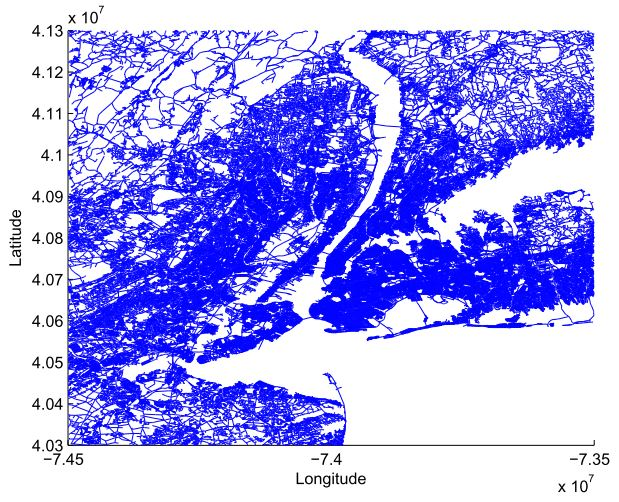
\includegraphics[width=1\linewidth]{Images/Chapter7/NY} 
    \caption{Rendering of NY city map} 
    \label{fig:7-1} 
    %\vspace{4ex}
  \end{minipage}%%
\hspace{5mm}
  \begin{minipage}[b]{0.45\linewidth}
    \centering
    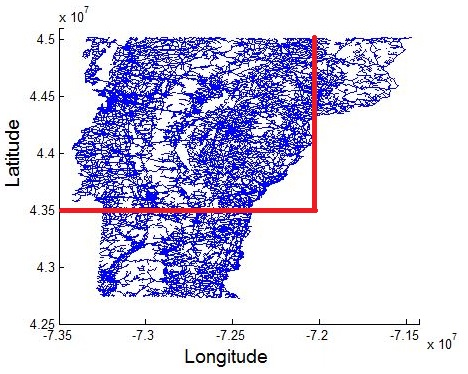
\includegraphics[width=1\linewidth]{Images/Chapter7/VTcut} 
    \caption{Cut of Vermont map (squared)} 
	 \label{fig:7-2}
	%\vspace{4ex}
  \end{minipage} 
\end{figure}

We selected the first twenty problems for the New York city road map proposed in \cite{Machuca2012}. These problems were randomly generated using an uniform distribution to select start and destination nodes. In a similar manner, we generated twenty random problems for the VT$_{cut}$ map. These test sets and the additional generated map files are available online\footnote{http://alef.iaia.lcc.uma.es/projects/alef-public/wiki/Benchmarks}. 
%Only algorithms \namoate \ and \namoalin \ are reported over these sets, since \namoalin \ clearly outperforms \namoalex.

Since previously reported runtimes of \namoa \ solving a biobjective version of these problems (minimizing  $c_2$ and $c_3$, i.e. much easier problems) were up to several days \citep{Machuca2011a}, we also established a runtime limit of 8 hours for the experiments over the NY city map. 

The algorithms were implemented in Common Lisp using LispWorks Professional 6.01 (64-bit), and run on a Sun Fire X4140 server with 2 six-core AMD Opteron 2435 at 2.60 GHz processors and 64 GB of DDR2 RAM memory. This machine is slower than the one employed to solve the random grid experiments, however, it was chosen due to the greater memory space requirements of the problem analyzed here. All experiments were run on a single thread.

In the following, we conduct an experimental evaluation of the algorithms in an analogous fashion of that performed in Chapter \ref{chapEmpiricalAnalysisGrids} for random grid problems.

%-------------------------------------------------------------------
\section{\texorpdfstring{\lexgo}{LEXGO*} \ vs \texorpdfstring{\namoa}{NAMOA*}}
\label{chapEmpiricalAnalysis:sec:resultsdimacslexgo}
%-------------------------------------------------------------------

This section analyzes \namoa \ and \lexgo on the realistic road maps of Vermont and New York city. The study is applied to the lexicographic and linear selection orders (see Definitions \ref{chapMultiObjAlg:def:lexorder} and \ref{chapMultiObjAlg:def:linorder} for further description), and performed over the two classes of experiments already described for random grids in Section \ref{chapEmpiricalAnalysis:sec:grids}.

The full set of experiments on Vermont was solved by all the algorithms, however, out of the twenty problems which compose the problem set of New York city, \namoalex \ and \namoalin \ were capable of solving only four of them, NY\#2, NY\#4, NY\#5 and NY\#16. The comparison to their \lexgo \ counterpart using the same selection order follows.
 
%-------------------------------------------------------------------
\subsection{Analysis on class I experiments}
\label{chapEmpiricalAnalysis:subsec:analysisdimacslexgoc1}
%-------------------------------------------------------------------

Target values for \lexgo \ were defined as in Equation \ref{eq:targets} for random grids class I experiments. Table \ref{tab:7-2} displays the percentage of goal-optimal solution vectors returned by \lexgo \ relative to the full set ($C^*$) returned by \namoa. 

\begin{table}
\caption{Class I experiments in road maps, percentage of goal-optimal solution vectors relative to $C^*$ for solvable problems within the time limit by \lexgo \ and \namoa. An asterisk ($^*$) indicates that the goals could not be satisfied.}
\label{tab:7-2}
\centering
\begin{tabular}{crrrrrrrr}
\hline \noalign{\smallskip}
& & & \multicolumn{5}{c}{\lexgo} \\
\noalign{\smallskip} \cline{4-8} \noalign{\smallskip}
& & \namoa & 1 & 0.75 & 0.5 & 0.25 & 0 & $k_1$\\
\noalign{\smallskip} 
 & $n$ & $|C^*|$ & \% & \% & \% & \% & \% & \\
\cline{1-8} \noalign{\smallskip} 
\parbox[t]{2mm}{\multirow{20}{*}{\rotatebox[origin=c]{90}{Vermont}}} & 1 & 1,252 & 100 & 3.04 & 0.64 & $^*$0.08 & $^*$0.08 \\
& 2 & 223 & 100 & 38.57 & 34.53 & $^*$0.45 & $^*$0.45 \\
& 3 & 34 & 100 & 67.65 & 29.41 & $^*$2.94 & $^*$2.94 \\
& 4 & 4,759 & 100 & 57.11 & 17.42 & $^*$0.02 & $^*$0.02 \\
& 5 & 334 & 100 & 36.23 & 1.80 & $^*$0.30 & $^*$0.30 \\
& 6 & 7,576 & 100 & 84.52 & 19.97 & $^*$0.01 & $^*$0.01 \\
& 7 & 3 & 100 & 33.33 & $^*$33.33 & $^*$33.33 & $^*$33.33 \\
& 8 & 5 & 100 & 60.00 & 20.00 & $^*$20.00 & $^*$20.00 \\
& 9 & 206 & 100 & 47.09 & 23.30 & $^*$0.49 & $^*$0.49 \\
& 10 & 9,712 & 100 & 82.22 & 20.15 & $^*$0.01 & $^*$0.01 \\
& 11 & 14,537 & 100 & 54.95 & 48.81 & $^*$0.01 & $^*$0.01 \\
& 12 & 1,648 & 100 & 32.52 & $^*$0.06 & $^*$0.06 & $^*$0.06 \\
& 13 & 10,256 & 100 & 92.82 & 43.80 & $^*$0.01 & $^*$0.01 \\
& 14 & 444 & 100 & 55.41 & 21.17 & $^*$0.23 & $^*$0.23 \\
& 15 & 1,310 & 100 & 49.16 & 4.81 & $^*$0.08 & $^*$0.08 \\
& 16 & 1,216 & 100 & 1.64 & $^*$0.08 & $^*$0.08 & $^*$0.08 \\
& 17 & 8,189 & 100 & 58.30 & 23.70 & $^*$0.01 & $^*$0.01 \\
& 18 & 38 & 100 & 65.79 & 18.42 & $^*$2.63 & $^*$2.63 \\
& 19 & 1 & 100 & 100.00 & 100.00 & 100.00 & 100.00 \\
& 20 & 4,949 & 100 & 33.97 & 9.23 & $^*$0.02 & $^*$0.02 \\
\noalign{\medskip}
\parbox[t]{2mm}{\multirow{4}{*}{\rotatebox[origin=c]{90}{NY city}}} & 2 & 303 & 100 & 57.42 & 4.62 & $^*$0.33 & $^*$0.33 \\
& 4 & 4,429 & 100 & 88.82 & 74.32 & $^*$0.02 & $^*$0.02 \\
& 5 & 7 & 100 & 71.42 & $^*$14.28 & $^*$14.28 & $^*$14.28 \\
& 16 & 1,640 & 100 & 48.35 & $^*$0.06 & $^*$0.06 & $^*$0.06 \\
\hline
\end{tabular}
\end{table}

Table \ref{tab:7-3} shows the relative percentage number of scanned labels by \lexgolin \ to \namoalin in Vermont and NY city maps. As it was mentioned before, the number of explored labels by \namoalin \ is nearly the same as \namoalex. This slight difference is attributed to the \emph{lazy filtering} procedure applied to both alternatives. This is also the case of \lexgolex \ and \lexgolin.

\begin{table}
\caption{Class I experiments in road maps, relative percentage number of scanned labels by \lexgolin \ to \namoalin.}
\label{tab:7-3}
\centering
\begin{tabular}{crrrrrrrr}
\hline \noalign{\smallskip}
& & & \multicolumn{5}{c}{\lexgolin} \\
\noalign{\smallskip} \cline{4-8} \noalign{\smallskip}
& & \namoalin & 1 & 0.75 & 0.5 & 0.25 & 0 & \multicolumn{1}{c}{$k_1$}\\
\noalign{\smallskip} 
 & $n$ & $\sum G_{cl}$ & \% & \% & \% & \% & \% & \\
\cline{1-8} \noalign{\smallskip} 
\parbox[t]{2mm}{\multirow{20}{*}{\rotatebox[origin=c]{90}{Vermont}}} & 1 & 211,268 & 99.73 & 46.80 & 11.63 & 4.05 & 0.07 \\ 
& 2 & 115,435 & 99.99 & 50.41 & 43.08 & 17.81 & 0.44 \\ 
& 3 & 11,332 & 96.86 & 83.15 & 49.28 & 15.91 & 2.06 \\ 
& 4 & 1,134,467 & 99.99 & 80.17 & 32.35 & 2.95 & 0.03 \\ 
& 5 & 45,650 & 96.65 & 72.95 & 16.58 & 3.59 & 1.65 \\ 
& 6 & 5,497,553 & 99.17 & 93.42 & 44.25 & 2.88 & 0.01 \\ 
& 7 & 187 & 73.26 & 55.61 & 55.08 & 57.75 & 45.99 \\ 
& 8 & 480 & 88.33 & 61.46 & 33.96 & 22.29 & 22.08 \\ 
& 9 & 65,140 & 99.76 & 67.24 & 39.98 & 15.10 & 0.71 \\ 
& 10 & 5,332,256 & 98.31 & 86.29 & 33.43 & 9.20 & 0.02 \\ 
& 11 & 10,125,074 & 98.27 & 72.55 & 69.46 & 19.64 & 0.02 \\ 
& 12 & 127,611 & 97.45 & 29.81 & 5.49 & 3.33 & 0.54 \\ 
& 13 & 8,664,536 & 99.98 & 97.45 & 70.83 & 20.19 & 0.01 \\ 
& 14 & 47,215 & 99.30 & 76.21 & 34.57 & 4.91 & 0.19 \\ 
& 15 & 571,195 & 99.95 & 93.83 & 68.61 & 3.35 & 0.21 \\ 
& 16 & 88,699 & 96.76 & 47.69 & 33.91 & 20.55 & 0.44 \\ 
& 17 & 1,223,581 & 99.60 & 73.43 & 26.25 & 4.96 & 0.16 \\ 
& 18 & 11,021 & 76.33 & 52.55 & 36.53 & 13.51 & 2.79 \\ 
& 19 & 92 & 64.13 & 64.13 & 64.13 & 64.13 & 64.13 \\ 
& 20 & 1,904,080 & 99.99 & 71.65 & 39.55 & 11.26 & 0.03 \\
\noalign{\medskip}
\parbox[t]{2mm}{\multirow{4}{*}{\rotatebox[origin=c]{90}{NY city}}} &
2 & 17,294 & 93.96 & 61.91 & 17.83 & 2.80 & 3.64 \\
& 4 & 3,390,656 & 99.40 & 92.23 & 74.00 & 9.14 & 0.01 \\
& 5 & 719 & 47.98 & 32.96 & 10.43 & 6.53 & 8.20 \\
& 16 & 2,445,191 & 81.14 & 47.17 & 11.67 & 0.53 & 0.01 \\ 
\hline
\end{tabular}
\end{table}

Finally, Tables \ref{tab:7-4} and \ref{tab:7-5} display the runtimes of \namoa \ and the relative time of \lexgo \ to \namoa \ for the maps of Vermont and NY city with the lexicographic and linear selection orders, respectively. When the runtime of \namoa \ was smaller than 0.01 seconds, we display $<0.01$ in the tables, and complete the relative percentages of \lexgo \ with dashes to indicate that those are not significative. Likewise, if the relative percentage of runtime of \lexgo \ to \namoa \ was smaller than 0.01\%, we simply display $<0.01$.

\begin{table}
\caption{Class I experiments in road maps, relative percentage runtimes in seconds for \lexgolex \ and \namoalex.}
\label{tab:7-4}
\centering
\begin{tabular}{crrrrrrrr}
\hline \noalign{\smallskip}
& & & \multicolumn{5}{c}{\lexgolex} \\
\noalign{\smallskip} \cline{4-8} \noalign{\smallskip}
& & \namoalex & 1 & 0.75 & 0.5 & 0.25 & 0 & \multicolumn{1}{c}{$k_1$}\\
\noalign{\smallskip} 
 & $n$ & Runtime (s) & \% & \% & \% & \% & \% & \\
\cline{1-8} \noalign{\smallskip} 
\parbox[t]{2mm}{\multirow{20}{*}{\rotatebox[origin=c]{90}{Vermont}}} & 1 & 39.95 & 106.68 & 16.20 & 3.12 & 1.21 & 0.04 \\ 
& 2 & 7.05 & 118.81 & 41.81 & 32.29 & 18.81 & 0.67 \\ 
& 3 & 0.32 & 137.80 & 117.18 & 58.43 & 18.90 & <0.01 \\ 
& 4 & 1,386.53 & 99.14 & 59.88 & 7.81 & 0.28 & <0.01 \\ 
& 5 & 2.49 & 111.26 & 66.23 & 22.52 & 2.48 & 2.52 \\ 
& 6 & 17,731.38 & 95.35 & 76.09 & 12.22 & 0.18 & <0.01 \\ 
& 7 & <0.01 & - & - & - & - & - \\ 
& 8 & <0.01 & - & - & - & - & - \\ 
& 9 & 3.60 & 121.23 & 61.48 & 28.56 & 16.46 & 0.42 \\ 
& 10 & 17,828.99 & 100.05 & 73.27 & 6.57 & 1.62 & <0.01 \\ 
& 11 & 30,318.76 & 99.85 & 57.99 & 47.17 & 2.77 & <0.01 \\ 
& 12 & 40.21 & 97.90 & 11.09 & 1.09 & 0.85 & 0.04 \\ 
& 13 & 29,337.51 & 104.79 & 97.68 & 38.46 & 7.92 & <0.01 \\ 
& 14 & 3.83 & 102.84 & 68.71 & 26.81 & 3.26 & <0.01 \\ 
& 15 & 115.33 & 102.54 & 83.58 & 42.54 & 0.78 & 0.03 \\ 
& 16 & 8.54 & 94.53 & 18.61 & 18.25 & 8.57 & <0.01 \\ 
& 17 & 2,245.32 & 96.76 & 44.88 & 5.07 & 0.39 & <0.01 \\ 
& 18 & 0.34 & 104.66 & 113.70 & 40.82 & 18.37 & <0.01 \\ 
& 19 & <0.01 & - & - & - & - & - \\ 
& 20 & 1,899.15 & 95.95 & 33.55 & 7.18 & 2.23 & <0.01 \\
\noalign{\medskip}
\parbox[t]{2mm}{\multirow{4}{*}{\rotatebox[origin=c]{90}{NY city}}} &
2 & 1.48 & 97.97 & 54.72 & 15.54 & 0.67 & 0.67 \\
& 4 & 4,752.77 & 101.94 & 84.97 & 59.52 & 1.57 & <0.01 \\
& 5 & <0.01 & - & - & - & - & - \\
& 16 & 559.76 & 81.93 & 41.86 & 11.30 & 0.18 & <0.01 \\
\hline
\end{tabular}
\end{table}

\begin{table}
\caption{Class I experiments in road maps, relative percentage runtimes in seconds for \lexgolin \ and \namoalin.}
\label{tab:7-5}
\centering
\begin{tabular}{crrrrrrrr}
\hline \noalign{\smallskip}
& & & \multicolumn{5}{c}{\lexgolin} \\
\noalign{\smallskip} \cline{4-8} \noalign{\smallskip}
& & \namoalin & 1 & 0.75 & 0.5 & 0.25 & 0 & \multicolumn{1}{c}{$k_1$}\\
\noalign{\smallskip} 
 & $n$ & Runtime (s) & \% & \% & \% & \% & \% & \\
\cline{1-8} \noalign{\smallskip} 
\parbox[t]{2mm}{\multirow{20}{*}{\rotatebox[origin=c]{90}{Vermont}}} &
1 & 40.02 & 98.71 & 20.78 & 4.80 & 1.29 & 0.04 \\ 
& 2 & 7.35 & 125.05 & 47.35 & 42.46 & 22.71 & 0.22 \\ 
& 3 & 0.30 & 194.93 & 166.66 & 94.59 & 26.35 & 5.41 \\ 
& 4 & 1,428.44 & 88.94 & 55.66 & 7.46 & 0.33 & <0.01 \\ 
& 5 & 2.62 & 136.28 & 97.02 & 19.65 & 2.40 & 1.18 \\ 
& 6 & 17,913.28 & 90.27 & 77.75 & 12.81 & 0.19 & <0.01 \\ 
& 7 & <0.01 & - & - & - & - & - \\ 
& 8 & <0.01 & - & - & - & - & - \\ 
& 9 & 3.42 & 131.02 & 73.95 & 45.22 & 21.45 & 0.91 \\ 
& 10 & 17,167.54 & 100.51 & 70.97 & 8.03 & 1.83 & <0.01 \\ 
& 11 & 28,712.69 & 96.00 & 52.18 & 42.35 & 3.83 & <0.01 \\ 
& 12 & 39.25 & 106.76 & 12.44 & 1.31 & 0.60 & 0.20 \\ 
& 13 & 27,556.06 & 101.59 & 95.62 & 34.33 & 9.40 & <0.01 \\ 
& 14 & 3.88 & 127.32 & 91.99 & 35.35 & 4.02 & <0.01 \\ 
& 15 & 108.65 & 102.89 & 93.65 & 60.95 & 1.38 & 0.04 \\ 
& 16 & 7.64 & 109.59 & 28.98 & 21.23 & 15.50 & 0.20 \\ 
& 17 & 2,077.78 & 100.42 & 51.94 & 5.04 & 0.48 & <0.01 \\ 
& 18 & 0.52 & 93.79 & 96.89 & 45.44 & 12.23 & 3.11 \\ 
& 19 & <0.01 & - & - & - & - & - \\ 
& 20 & 1,699.91 & 104.33 & 29.30 & 9.66 & 2.87 & <0.01 \\ 
\noalign{\medskip}
\parbox[t]{2mm}{\multirow{4}{*}{\rotatebox[origin=c]{90}{NY city}}} &
2 & 1.43 & 129.37 & 86.01 & 25.87 & 2.09 & 0.69 \\
& 4 & 3,963.98 & 110.34 & 105.57 & 85.97 & 4.35 & <0.01 \\
& 5 & <0.01 & - & - & - & - & - \\
& 16 & 712.59 & 71.32 & 52.04 & 11.02 & 0.14 & <0.01 \\
\hline
\end{tabular}
\end{table}

The results obtained for the road map problems are much more heterogeneous than the ones for random grids. Thus, we can observe a wide range of goal-optimal solution ratios, for instance, the range of ratios of goal-optimal solution vectors returned for $k_1 = 0.75$ varies from 1.64\% to 92.82\% (see Table \ref{tab:7-2}) for Vermont map problems (VT\#16 and VT\#13, respectively). This could be expected, since the road map experiments represent a realistic scenario, on the contrary, the random grids were generated using an uniform distribution. However, both scenarios share the inability to satisfy the goals when $k_1 = 0.25$ or $k_1 = 0$.

The heterogeneity of the results remains regarding the labels scanned and the runtime of \lexgo, however, it shall be noticed that the runtime comparison between \namoalex \ and \namoalin \ does not show a clear advantage to \namoalin, as it happens in the grids experiments. 

Regarding the lexicographic order, \lexgo \ does perform in a very similar manner for the road maps as for the random grids. \lexgo \ explores for the most difficult problem solved by both algorithms, VT\#11 of Vermont, 98.27\%, 72.55\% and 69.46\% of the labels explored by \namoa \ for $k_1=1$, $k_1=0.75$ and $k_1=0.5$, respectively. 

The small time overhead observed in grid experiments for $k_1=1$ is also found in some of the road map experiments, as well as the important reductions in labels scanned and runtimes when $k_1 = 0.25$ or $k_1 = 0$, regardless the function employed as selection order.

We will further analyze in depth these data and the class II experiments reported below in the summary section. 

%-------------------------------------------------------------------
\subsection{Analysis on class II experiments}
\label{chapEmpiricalAnalysis:subsec:analysisdimacslexgoc2}
%-------------------------------------------------------------------

In the second class of experiments, goal preferences and target values were defined using $k_1 = \{0.75 , 0.5\}$ with all possible values of $k_2$ defined in Equation \ref{eq:targets2}. Tables \ref{tab:7-6} displays the relative number of goal-optimal solution vectors to the full Pareto set. The number of scanned labels for these maps is shown in Table \ref{tab:7-7}. Finally, Tables \ref{tab:7-8} and \ref{tab:7-9} show runtimes of \lexgo \ and \namoa \ with lexicographic and linear selection orders, respectively.

There are several cases where the solution returned is exactly the same. When problems NY\#5 and NY\#16 are solved with $k_1=0.5$ the only solution returned, the one which minimizes the deviation from goals, is the same for all values of $k_2$. 

It can be observed that both, \lexgolin \ and \lexgolex, outperform their \namoa \ counterparts when either $k_1=0.75$ or $k_1=0.5$, except for the problem VT\#3.

\begin{table}
\caption{Class II experiments in road maps, \lexgo \ percentage of goal-optimal solution vectors relative to the size of $C^*$. An asterisk ($^*$) indicates that the goals could not be satisfied.}
\label{tab:7-6}
\centering
\scalebox{.86}{
\begin{tabular}{crrrrrrrrrrr}
\hline \noalign{\smallskip}
& & & \multicolumn{8}{c}{\lexgo} & \\
\noalign{\smallskip} \cline{4-11}
\multicolumn{3}{c}{} & \multicolumn{4}{c|}{0.75} & \multicolumn{4}{c}{0.5} & \multicolumn{1}{c}{$k_1$}\\
& & \namoa & 0.75 & 0.5625 & 0.375 & \multicolumn{1}{c|}{0.1875} & 0.5 & 0.375 & 0.25 & 0.125 & \multicolumn{1}{c}{$k_2$}\\
\noalign{\smallskip} 
& $n$ & $|C^*|$ & \% & \% & \% & \% & \% & \% & \% & \% & \\
\cline{1-11} \noalign{\smallskip} 
\parbox[t]{2mm}{\multirow{20}{*}{\rotatebox[origin=c]{90}{Vermont}}} &
1 & 1,252 & 3.04 & 3.04 & 0.32 & 0.08 & 0.64 & 0.08 & 0.08 & 0.08 \\ 
& 2 & 223 & 38.57 & 36.77 & 24.66 & 14.80 & 34.53 & 24.66 & 15.70 & 11.21 \\ 
& 3 & 34 & 67.65 & 64.71 & 55.88 & 35.29 & 29.41 & 20.59 & 5.88 & 2.94 \\ 
& 4 & 4,759 & 57.11 & 54.32 & 29.57 & 8.01 & 17.42 & 6.41 & 1.41 & 0.02 \\ 
& 5 & 334 & 36.23 & 24.25 & 12.28 & 0.30 & 1.80 & 0.30 & 0.30 & 0.30 \\ 
& 6 & 7,576 & 84.52 & 68.99 & 42.56 & 9.75 & 19.97 & 6.89 & 0.01 & 0.01 \\ 
& 7 & 3 & 33.33 & 33.33 & 33.33 & 33.33 & 33.33 & 33.33 & 33.33 & 33.33 \\ 
& 8 & 5 & 60.00 & 20.00 & 20.00 & 20.00 & 20.00 & 20.00 & 20.00 & 20.00 \\ 
& 9 & 206 & 47.09 & 36.89 & 30.58 & 16.50 & 23.30 & 22.33 & 16.02 & 0.49 \\ 
& 10 & 9,712 & 82.22 & 49.24 & 14.93 & 1.01 & 20.15 & 4.17 & 0.01 & 0.01 \\ 
& 11 & 14,537 & 54.95 & 53.64 & 42.46 & 21.73 & 48.81 & 39.85 & 23.66 & 7.36 \\ 
& 12 & 1,648 & 32.52 & 31.98 & 31.98 & 18.63 & 0.06 & 0.06 & 0.06 & 0.06 \\ 
& 13 & 10,256 & 92.82 & 89.12 & 53.64 & 20.69 & 43.80 & 22.24 & 13.31 & 0.09 \\ 
& 14 & 444 & 55.41 & 49.77 & 33.56 & 3.60 & 21.17 & 7.88 & 0.68 & 0.23 \\ 
& 15 & 1,310 & 49.16 & 34.43 & 28.24 & 14.73 & 4.81 & 4.12 & 2.82 & 0.08 \\ 
& 16 & 1,216 & 1.64 & 0.08 & 0.08 & 0.08 & 0.08 & 0.08 & 0.08 & 0.08 \\ 
& 17 & 8,189 & 58.30 & 55.50 & 32.34 & 3.04 & 23.70 & 8.19 & 0.10 & 0.01 \\ 
& 18 & 38 & 65.79 & 65.79 & 47.37 & 42.11 & 18.42 & 10.53 & 10.53 & 2.63 \\ 
& 19 & 1 & 100.00 & 100.00 & 100.00 & 100.00 & 100.00 & 100.00 & 100.00 & 100.00 \\ 
& 20 & 4,949 & 33.97 & 25.16 & 15.15 & 0.02 & 9.23 & 2.61 & 0.02 & 0.02 \\ 
\noalign{\medskip}
\parbox[t]{2mm}{\multirow{4}{*}{\rotatebox[origin=c]{90}{NY city}}} &
2 & 303 & 57.42 & 50.49 & 30.69 & $^*$0.33 & 4.62 & $^*$0.33 & $^*$0.33 & $^*$0.33 \\
& 4 & 4,429 & 88.82 & 87.76 & 70.28 & 8.19 & 74.32 & 63.44 & 21.49 & 0.29 \\
& 5 & 7 & 71.42 & 42.85 & 28.57 & $^*$14.28 & $^*$14.28 & $^*$14.28 & $^*$14.28 & $^*$14.28 \\
& 16 & 1,640 & 48.53 & 17.98 & 3.04 & $^*$0.06 & $^*$0.06 & $^*$0.06 & $^*$0.06 & $^*$0.06 \\
\hline
\end{tabular}
}
\end{table} 

\begin{table}
\caption{Class II experiments in road maps, relative number of scanned labels by \lexgo \ and \namoa \ on lexicographic selection order.}
\label{tab:7-7}
\centering
\scalebox{.9}{
\begin{tabular}{crrrrrrrrrrr}
\hline \noalign{\smallskip}
& & & \multicolumn{8}{c}{\lexgolin} & \\
\noalign{\smallskip} \cline{4-11}
\multicolumn{3}{c}{} & \multicolumn{4}{c|}{0.75} & \multicolumn{4}{c}{0.5} & \multicolumn{1}{c}{$k_1$}\\
& & \namoalin & 0.75 & 0.5625 & 0.375 & \multicolumn{1}{c|}{0.1875} & 0.5 & 0.375 & 0.25 & 0.125 & \multicolumn{1}{c}{$k_2$}\\
\noalign{\smallskip} 
& $n$ & $\sum G_{cl}$ & \% & \% & \% & \% & \% & \% & \% & \% & \\
\cline{1-11} \noalign{\smallskip} 
\parbox[t]{2mm}{\multirow{20}{*}{\rotatebox[origin=c]{90}{Vermont}}} &
1 & 211,268 & 46.80 & 44.21 & 33.78 & 31.55 & 11.63 & 9.91 & 9.91 & 9.91 \\ 
& 2 & 115,435 & 50.41 & 49.98 & 43.35 & 32.32 & 43.08 & 37.83 & 30.73 & 19.11 \\ 
& 3 & 11,332 & 83.15 & 78.08 & 72.31 & 43.98 & 49.28 & 44.98 & 26.45 & 23.01 \\ 
& 4 & 1,134,467 & 80.17 & 79.10 & 54.28 & 25.85 & 32.35 & 15.50 & 4.90 & 3.69 \\ 
& 5 & 45,650 & 72.95 & 61.01 & 32.07 & 16.42 & 16.58 & 11.82 & 11.41 & 11.41 \\ 
& 6 & 5,497,553 & 93.42 & 83.51 & 55.34 & 14.48 & 44.25 & 28.19 & 8.94 & 8.94 \\ 
& 7 & 187 & 55.61 & 55.61 & 55.61 & 55.61 & 55.08 & 55.08 & 55.08 & 55.08 \\ 
& 8 & 480 & 61.46 & 47.29 & 22.29 & 22.08 & 33.96 & 22.29 & 22.08 & 22.08 \\ 
& 9 & 65,140 & 67.24 & 61.04 & 45.71 & 32.52 & 39.98 & 32.14 & 26.18 & 11.74 \\ 
& 10 & 5,332,256 & 86.29 & 63.39 & 26.69 & 4.26 & 33.43 & 13.75 & 5.17 & 5.17 \\ 
& 11 & 10,125,074 & 72.55 & 72.24 & 68.17 & 40.86 & 69.46 & 65.85 & 51.88 & 19.27 \\ 
& 12 & 127,611 & 29.81 & 26.58 & 26.54 & 15.69 & 5.49 & 5.49 & 5.49 & 5.49 \\ 
& 13 & 8,664,536 & 97.45 & 97.09 & 84.46 & 27.20 & 70.83 & 60.09 & 31.32 & 1.89 \\ 
& 14 & 47,215 & 76.21 & 66.15 & 37.68 & 7.09 & 34.57 & 18.48 & 3.60 & 2.37 \\ 
& 15 & 571,195 & 93.83 & 87.18 & 75.67 & 56.63 & 68.61 & 60.84 & 52.78 & 28.48 \\ 
& 16 & 88,699 & 47.69 & 41.25 & 41.25 & 41.25 & 33.91 & 33.91 & 33.91 & 33.91 \\ 
& 17 & 1,223,581 & 73.43 & 71.77 & 57.03 & 20.66 & 26.25 & 14.31 & 1.89 & 1.66 \\ 
& 18 & 11,021 & 52.55 & 52.21 & 49.68 & 46.14 & 36.53 & 35.68 & 35.01 & 31.46 \\ 
& 19 & 92 & 64.13 & 64.13 & 64.13 & 64.13 & 64.13 & 64.13 & 64.13 & 64.13 \\ 
& 20 & 1,904,080 & 71.65 & 66.27 & 46.16 & 16.18 & 39.55 & 24.51 & 11.51 & 11.51 \\ 
\noalign{\medskip}
\parbox[t]{2mm}{\multirow{4}{*}{\rotatebox[origin=c]{90}{NY city}}} &
2 & 17,294 & 61.91 & 53.45 & 32.15 & 6.74 & 17.83 & 12.25 & 12.25 & 12.25 \\
& 4 & 3,390,656 & 92.23 & 91.91 & 82.21 & 25.98 & 74.00 & 67.66 & 44.58 & 7.05 \\
& 5 & 719 & 32.96 & 25.45 & 17.80 & 9.59 & 10.43 & 10.43 & 10.43 & 10.43 \\
& 16 & 2,445,191 & 47.17 & 25.79 & 9.41 & 2.76 & 11.67 & 11.67 & 11.67 & 11.67 \\
\hline
\end{tabular}
}
\end{table} 

\begin{table}
\caption{Class II experiments in road maps, runtimes in seconds of \namoalex \ and \lexgolex \ percentage of runtime compared to \namoalex.}
\label{tab:7-8}
\centering
\scalebox{.9}{
\begin{tabular}{crrrrrrrrrrr}
\hline \noalign{\smallskip}
& & & \multicolumn{8}{c}{\lexgolex} & \\
\noalign{\smallskip} \cline{4-11}
\multicolumn{3}{c}{} & \multicolumn{4}{c|}{0.75} & \multicolumn{4}{c}{0.5} & \multicolumn{1}{c}{$k_1$}\\
& & \namoalex & 0.75 & 0.5625 & 0.375 & \multicolumn{1}{c|}{0.1875} & 0.5 & 0.375 & 0.25 & 0.125 & \multicolumn{1}{c}{$k_2$}\\
\noalign{\smallskip} 
& $n$ & Runtime (s) & \% & \% & \% & \% & \% & \% & \% & \% & \\
\cline{1-11} \noalign{\smallskip} 
\parbox[t]{2mm}{\multirow{20}{*}{\rotatebox[origin=c]{90}{Vermont}}} &
1 & 39.95 & 16.20 & 16.01 & 18.04 & 32.95 & 3.12 & 3.71 & 4.06 & 5.15 \\ 
& 2 & 7.05 & 41.81 & 43.37 & 33.19 & 30.76 & 32.29 & 27.43 & 25.88 & 17.03 \\ 
& 3 & 0.32 & 117.18 & 104.57 & 97.5 & 52.13 & 58.43 & 52.44 & 29.06 & 28.66 \\ 
& 4 & 1,386.53 & 59.88 & 62.11 & 23.77 & 4.94 & 7.81 & 1.45 & 0.25 & 0.32 \\ 
& 5 & 2.49 & 66.23 & 56.85 & 41.87 & 25.64 & 22.52 & 9.98 & 12.5 & 21.23 \\ 
& 6 & 17,731.38 & 76.09 & 56.61 & 23.61 & 1.25 & 12.22 & 4.62 & 0.74 & 1.59 \\ 
& 7 & <0.01 & - & - & - & - & - & - & - & - \\ 
& 8 & <0.01 & - & - & - & - & - & - & - & - \\ 
& 9 & 3.60 & 61.48 & 55.87 & 41.99 & 25.53 & 28.56 & 27.70 & 20.79 & 14.29 \\ 
& 10 & 17,828.99 & 73.27 & 29.91 & 3.95 & 0.19 & 6.57 & 1.15 & 0.41 & 0.75 \\ 
& 11 & 30,318.76 & 57.99 & 56.67 & 42.22 & 16.53 & 47.17 & 38.78 & 24.12 & 4.01 \\ 
& 12 & 40.21 & 11.09 & 9.12 & 9.62 & 4.15 & 1.09 & 1.09 & 1.05 & 1.09 \\ 
& 13 & 29,337.51 & 97.68 & 91.96 & 53.87 & 6.39 & 38.46 & 22.80 & 6.83 & 0.08 \\ 
& 14 & 3.83 & 68.71 & 57.30 & 38.61 & 7.71 & 26.81 & 12.19 & 1.64 & 1.64 \\ 
& 15 & 115.33 & 83.58 & 75.59 & 53.82 & 36.58 & 42.54 & 35.66 & 31.07 & 16.96 \\ 
& 16 & 8.54 & 18.61 & 18.43 & 23.00 & 22.27 & 18.25 & 17.71 & 15.51 & 16.42 \\ 
& 17 & 2,245.32 & 44.88 & 41.85 & 21.15 & 2.45 & 5.07 & 1.11 & 0.06 & 0.05 \\ 
& 18 & 0.34 & 113.7 & 63.85 & 59.18 & 100.00 & 40.82 & 45.48 & 40.82 & 41.11 \\ 
& 19 & <0.01 & - & - & - & - & - & - & - & - \\ 
& 20 & 1,899.15 & 33.55 & 21.84 & 10.66 & 5.19 & 7.18 & 2.61 & 1.67 & 2.10 \\ 
\noalign{\medskip}
\parbox[t]{2mm}{\multirow{4}{*}{\rotatebox[origin=c]{90}{NY city}}} &
2 & 1.48 & 57.14 & 50.00 & 37.85 & 4.50 & 16.42 & 15.57 & 17.85 & 17.78 \\
& 4 & 4,752.77 & 84.97 & 85.43 & 55.18 & 5.61 & 59.52 & 39.85 & 13.19 & 0.86 \\
& 5 & <0.01 & - & - & - & - & - & - & - & - \\
& 16 & 559.76 & 41.86 & 21.77 & 5.92 & 2.26 & 11.29 & 13.91 & 15.06 & 15.30 \\
\hline
\end{tabular}
}
\end{table} 

\begin{table}
\caption{Class II experiments in road maps, runtimes in seconds of \namoalin \ and \lexgolin \ percentage of runtime compared to \namoalin.}
\label{tab:7-9}
\centering
\scalebox{.88}{
\begin{tabular}{crrrrrrrrrrr}
\hline \noalign{\smallskip}
& & & \multicolumn{8}{c}{\lexgolin} & \\
\noalign{\smallskip} \cline{4-11}
\multicolumn{3}{c}{} & \multicolumn{4}{c|}{0.75} & \multicolumn{4}{c}{0.5} & \multicolumn{1}{c}{$k_1$}\\
& & \namoalin & 0.75 & 0.5625 & 0.375 & \multicolumn{1}{c|}{0.1875} & 0.5 & 0.375 & 0.25 & 0.125 & \multicolumn{1}{c}{$k_2$}\\
\noalign{\smallskip} 
& $n$ & Runtime (s) & \% & \% & \% & \% & \% & \% & \% & \% & \\
\cline{1-11} \noalign{\smallskip} 
\parbox[t]{2mm}{\multirow{20}{*}{\rotatebox[origin=c]{90}{Vermont}}} &
1 & 40.01 & 20.78 & 21.17 & 37.66 & 42.61 & 4.80 & 5.03 & 5.30 & 5.65 \\ 
& 2 & 7.34 & 47.35 & 56.48 & 44.58 & 34.19 & 42.46 & 39.70 & 32.91 & 19.54 \\ 
& 3 & 0.29 & 221.28 & 231.76 & 147.64 & 153.04 & 94.59 & 84.12 & 52.70 & 42.23 \\ 
& 4 & 1,428.43 & 55.66 & 51.21 & 26.87 & 5.55 & 7.46 & 1.71 & 0.33 & 0.37 \\ 
& 5 & 2.62 & 97.02 & 82.14 & 73.83 & 41.09 & 19.65 & 13.70 & 21.40 & 15.45 \\ 
& 6 & 17,913.28 & 77.75 & 55.72 & 23.64 & 1.51 & 12.81 & 6.25 & 0.93 & 1.79 \\ 
& 7 & <0.01 & - & - & - & - & - & - & - & - \\ 
& 8 & <0.01 & - & - & - & - & - & - & - & - \\ 
& 9 & 3.41 & 73.95 & 71.20 & 49.31 & 36.99 & 45.22 & 38.34 & 26.92 & 12.79 \\ 
& 10 & 17,167.53 & 70.97 & 31.26 & 4.90 & 0.29 & 8.03 & 1.70 & 0.57 & 0.82 \\ 
& 11 & 28,712.68 & 52.18 & 48.93 & 42.12 & 19.42 & 42.35 & 37.41 & 25.37 & 5.52 \\ 
& 12 & 39.25 & 12.44 & 10.09 & 10.57 & 4.73 & 1.31 & 1.27 & 1.27 & 1.31 \\ 
& 13 & 27,556.06 & 95.62 & 87.11 & 62.33 & 7.95 & 34.33 & 26.01 & 8.44 & 0.13 \\ 
& 14 & 3.88 & 91.99 & 81.54 & 45.80 & 4.81 & 35.35 & 24.49 & 5.61 & 2.01 \\ 
& 15 & 108.65 & 93.65 & 94.52 & 73.55 & 74.26 & 60.95 & 56.35 & 57.83 & 38.00 \\ 
& 16 & 7.64 & 28.98 & 26.73 & 33.07 & 30.82 & 21.23 & 24.90 & 22.04 & 23.05 \\ 
& 17 & 2,077.77 & 51.94 & 46.93 & 22.64 & 3.21 & 5.04 & 1.40 & 0.07 & 0.08 \\ 
& 18 & 0.51 & 96.89 & 57.67 & 54.56 & 51.46 & 45.44 & 45.44 & 84.85 & 78.83 \\ 
& 19 & <0.01 & - & - & - & - & - & - & - & - \\
& 20 & 1,699.91 & 29.30 & 24.70 & 18.36 & 8.33 & 9.66 & 6.06 & 2.40 & 2.67 \\ 
\noalign{\medskip}
\parbox[t]{2mm}{\multirow{4}{*}{\rotatebox[origin=c]{90}{NY city}}} &
2 & 1.43 & 86.01 & 70.62 & 44.75 & 10.48 & 25.87 & 20.27 & 18.18 & 18.18 \\
& 4 & 3,963.98 & 105.57 & 106.69 & 106.50 & 19.23 & 85.97 & 71.12 & 44.33 & 3.73 \\
& 5 & <0.01 & - & - & - & - & - & - & - & - \\
& 16 & 712.59 & 52.04 & 30.86 & 7.84 & 2.12 & 11.02 & 12.47 & 13.04 & 13.47 \\
\hline
\end{tabular}
}
\end{table} 

%-------------------------------------------------------------------
\subsection{Summary}
\label{chapEmpiricalAnalysis:subsec:summarydimacslexgo}
%-------------------------------------------------------------------

We have analyzed the relative space and runtime performance of \lexgo \ over \namoa \ on road map problems. Two different functions to select the best alternative from the OPEN set have been also tested with both algorithms. Tables \ref{tab:7-10} and \ref{tab:7-11} summarize the outcome of the class I and class II experiments. 

In class I experiments, the number of goal-optimal solution vectors found when $k_1=0.75$ is slightly smaller than for the grid experiments, whereas it is slightly greater when $k_1=0.5$. The scanned labels follow the same trend.  

The experiments over random grids shown in Chapter \ref{chapEmpiricalAnalysisGrids} defined a clear advantage of the linear selection order over the lexicographic one when applied to \namoa. However, in our road map experiments, the practical advantage of \namoalin \ over \namoalex \ is greatly reduced to 4.3\% (see Tables \ref{tab:7-11a} and \ref{tab:7-11b}). 

The relative improvement of \lexgolin \ over \namoalin \ is enhanced in comparison with the results of grids. In those, the majority of the experiments in class II with $k_1=0.75$ could not achieve a runtime improvement over \namoalin. Nevertheless, \lexgolin \ in road maps achieves a relative improvement over \namoalin \ very similar to the improvement achieved by \lexgolex \ over \namoalex. 

\begin{table}
\caption{%
	Class I experiments in road maps, summary of the relative space and time performance of \lexgo \ over \namoa.
     }%
\vspace{0.05\textwidth}
\begin{center}
        \subtable[Relative average number of goal-optimal solution vectors for the Vermont problems]{%
\label{tab:7-10a}
\begin{tabular}{rrrrrrr}
\hline \noalign{\smallskip}
 & \multicolumn{5}{c}{\lexgo} \\
\noalign{\smallskip} \cline{2-6} \noalign{\smallskip}
\namoa & 1 & 0.75 & 0.5 & 0.25 & 0 & \multicolumn{1}{c}{$k_1$}\\
\noalign{\smallskip} 
Avg. $|C^*|$ & \% & \% & \% & \% & \% & \\
\cline{1-6} \noalign{\smallskip} 
3,334.6 & 100 & 64.34 & 27.89 & 0.03 & 0.03 \\
\hline
\end{tabular}
        }%
\vspace{0.05\textwidth} % To get a little bit of space between the figures
        \subtable[Relative average number of scanned labels for the Vermont problems]{%
\label{tab:7-10b}
\begin{tabular}{rrrrrrr}
\hline \noalign{\smallskip}
 & \multicolumn{5}{c}{\lexgolin} \\
\noalign{\smallskip} \cline{2-6} \noalign{\smallskip}
\namoalin & 1 & 0.75 & 0.5 & 0.25 & 0 & \multicolumn{1}{c}{$k_1$}\\
\noalign{\smallskip} 
Avg. $\sum G_{cl}$ & \% & \% & \% & \% & \% & \\
\cline{1-6} \noalign{\smallskip} 
1,758,843.6 & 99.06	& 84.15 & 55.12 & 13.60 & 0.04 \\
\hline
\end{tabular}
        }\\ %  ------- End of the first row ----------------------%
\vspace{0.05\textwidth}
        \subtable[Relative average time performance of \lexgolex \ to \namoalex \ for the Vermont problems]{%
\label{tab:7-10c}
\begin{tabular}{rrrrrrr}
\hline \noalign{\smallskip}
 & \multicolumn{5}{c}{\lexgolex} \\
\noalign{\smallskip} \cline{2-6} \noalign{\smallskip}
\namoalex & 1 & 0.75 & 0.5 & 0.25 & 0 & \multicolumn{1}{c}{$k_1$}\\
\noalign{\smallskip} 
Avg. runtime (s) & \% & \% & \% & \% & \% & \\
\cline{1-6} \noalign{\smallskip} 
5,048.47 & 100.39 & 74.67 & 29.06 & 3.51 & <0.01 \\
\hline
\end{tabular}
        }%  %  ------- End of the second row ----------------------%
\vspace{0.05\textwidth}
        \subtable[Relative average time performance of \lexgolin \ to \namoalin \ for the Vermont problems]{%
\label{tab:7-10d}
\begin{tabular}{rrrrrrr}
\hline \noalign{\smallskip}
 & \multicolumn{5}{c}{\lexgolin} \\
\noalign{\smallskip} \cline{2-6} \noalign{\smallskip}
\namoalin & 1 & 0.75 & 0.5 & 0.25 & 0 & \multicolumn{1}{c}{$k_1$}\\
\noalign{\smallskip} 
Avg. runtime (s) & \% & \% & \% & \% & \% & \\
\cline{1-6} \noalign{\smallskip} 
4,838.46    & 97.49 & 72.28 & 26.61 & 4.25 & <0.01 \\
\hline
\end{tabular}
        }%  %  ------- End of the third row ----------------------%
\end{center}
\label{tab:7-10}
\end{table}

\begin{table}
\caption{%
    Class II experiments in road maps, summary of the relative space and runtime performance of \lexgo \ over \namoa \ for the Vermont map experiments.
     }%
\vspace{0.05\textwidth}
\begin{center}
        \subtable[Relative average number of goal-optimal solution vectors]{%
\label{tab:7-11a}
\begin{tabular}{rrrrrrrrrr}
\hline \noalign{\smallskip}
& \multicolumn{8}{c}{\lexgo} & \\
\noalign{\smallskip} \cline{2-9}
\multicolumn{1}{c}{} & \multicolumn{4}{c|}{0.75} & \multicolumn{4}{c}{0.5} & \multicolumn{1}{c}{$k_1$}\\
\namoa & 0.75 & 0.5625 & 0.375 & \multicolumn{1}{c|}{0.1875} & 0.5 & 0.375 & 0.25 & 0.125 & \multicolumn{1}{c}{$k_2$}\\
\noalign{\smallskip} 
Avg. $|C^*|$ & \% & \% & \% & \% & \% & \% & \% & \% & \\
\cline{1-9} \noalign{\smallskip}  
3,334.6 & 64.34 &	55.25 & 33.59 & 11.04 &	27.89 & 15.47 & 7.50 & 1.68 \\
\hline
\end{tabular}
        }%
\vspace{0.05\textwidth} % To get a little bit of space between the figures
        \subtable[Relative average number of scanned labels]{%
\label{tab:7-11b}
\begin{tabular}{rrrrrrrrrr}
\hline \noalign{\smallskip}
& \multicolumn{8}{c}{\lexgolin} & \\
\noalign{\smallskip} \cline{2-9}
\multicolumn{1}{c}{} & \multicolumn{4}{c|}{0.75} & \multicolumn{4}{c}{0.5} & \multicolumn{1}{c}{$k_1$}\\
\namoalin & 0.75 & 0.5625 & 0.375 & \multicolumn{1}{c|}{0.1875} & 0.5 & 0.375 & 0.25 & 0.125 & \multicolumn{1}{c}{$k_2$}\\
\noalign{\smallskip} 
Avg. $\sum G_{cl}$ & \% & \% & \% & \% & \% & \% & \% & \% & \\
\cline{1-9} \noalign{\smallskip}  
1,758,843.6 & 84.15 & 78.37 & 61.34 & 25.29 & 55.12 & 43.97 & 26.89 & 9.74 \\
\hline
\end{tabular}
        }\\ %  ------- End of the first row ----------------------%
\vspace{0.05\textwidth}
        \subtable[Relative average runtime performance of \lexgolex \ to \namoalex]{%
\label{tab:7-11c}
\scalebox{.95}{
\begin{tabular}{rrrrrrrrrr}
\hline \noalign{\smallskip}
& \multicolumn{8}{c}{\lexgolex} & \\
\noalign{\smallskip} \cline{2-9}
\multicolumn{1}{c}{} & \multicolumn{4}{c|}{0.75} & \multicolumn{4}{c}{0.5} & \multicolumn{1}{c}{$k_1$}\\
\namoalex & 0.75 & 0.5625 & 0.375 & \multicolumn{1}{c|}{0.1875} & 0.5 & 0.375 & 0.25 & 0.125 & \multicolumn{1}{c}{$k_2$}\\
\noalign{\smallskip} 
Avg. runtime (s) & \% & \% & \% & \% & \% & \% & \% & \% & \\
\cline{1-9} \noalign{\smallskip}  
5,048.47 & 74.67 & 61.26 & 34.25 & 7.36 & 29.06 &19.43 & 9.51 & 1.71 \\
\hline
\end{tabular}
}
        }%  %  ------- End of the second row ----------------------%
\vspace{0.05\textwidth}
        \subtable[Relative average runtime performance of \lexgolin \ to \namoalin]{%
\label{tab:7-11d}
\scalebox{.92}{
\begin{tabular}{rrrrrrrrrr}
\hline \noalign{\smallskip}
& \multicolumn{8}{c}{\lexgolin} & \\
\noalign{\smallskip} \cline{2-9}
\multicolumn{1}{c}{} & \multicolumn{4}{c|}{0.75} & \multicolumn{4}{c}{0.5} & \multicolumn{1}{c}{$k_1$}\\
\namoalin & 0.75 & 0.5625 & 0.375 & \multicolumn{1}{c|}{0.1875} & 0.5 & 0.375 & 0.25 & 0.125 & \multicolumn{1}{c}{$k_2$}\\
\noalign{\smallskip} 
Avg. runtime (s) & \% & \% & \% & \% & \% & \% & \% & \% & \\
\cline{1-9} \noalign{\smallskip} 
4,838.46 & 72.28 & 57.51 & 36.81 & 8.77 & 26.61 & 20.20 & 10.33 & 2.26 \\
\hline
\end{tabular}
}
        }%  %  ------- End of the third row ----------------------%
\end{center}
\label{tab:7-11}
\end{table}

%-------------------------------------------------------------------
\section{\texorpdfstring{\namoate}{NAMOA*dr} \ vs \texorpdfstring{\namoa}{NAMOA*}}
\label{chapEmpiricalAnalysis:sec:resultsdimacsnamoate}
%-------------------------------------------------------------------

This section analyzes the runtime performance of the three different versions of the \namoa \ algorithm, \namoalex, \namoalin \ and \namoate. The experiments presented in this section analyze the impact of the dimensionality reduction technique on the sets of road map problems already presented.

The three versions of \namoa \ differ in the order of selection of OPEN labels and/or in the way dominance is checked in filtering and cl-pruning operations. The first and second variants are \namoalex \ and \namoalin, and both use, to the best of our knowledge, the usual dominance pruning and filtering technique in previously reported experimental evaluations of multiobjective search algorithms. The third algorithm analyzed, \namoate, uses a lexicographic order of selection and the t-discarding technique, described in Section \ref{chapMultiObjAlg:sec:Time-efficient-MSalg}, for filtering and cl-pruning.

%-------------------------------------------------------------------
\subsection{Analysis}
\label{chapEmpiricalAnalysis:subsec:analysisdimacsnamoate}
%-------------------------------------------------------------------

Tables \ref{tab:7-12} and \ref{tab:7-13} show the size of relevant label sets for each problem instance solved by \namoate, as well as \namoalin \ and \namoate \ runtimes for the NY city and Vermont maps, respectively. The first column displays the problem identifier ($n$). The description of these sets is the same presented previously in Table \ref{tab:6-6}. Notice that for NY map only problems solved within the time limit are displayed in this table. Figure \ref{fig:7-3} shows the runtimes in logarithmic scale of \namoalin \ and \namoate \ for VT$_{cut}$ map sorted by the number of scanned labels by each problem.

\begin{table}
\caption{Size of relevant sets of labels for VT$_{cut}$ road map experiments solved by \namoate}
\label{tab:7-12}
\begin{center}
\scalebox{.8}{
\begin{tabular}{crrrrrrrrr}
\cline{3-10} \noalign{\smallskip}
 & &  \multicolumn{6}{c}{Size of relevant sets of labels of \namoate} & \multicolumn{2}{c}{Runtime (sec)} \\
\noalign{\smallskip} \hline
\multicolumn{1}{c}{$n$} & Max OPEN & $\sum G_{cl}$ & $\sum T(G_{cl})$ & \% & $\text{C}^*$ & $T(\text{C}^*)$ & \% & $t_{\text{NAMOA}^* \text{lin}}$ & $t_{\text{NAMOA}^* \text{dr}}$\\
\hline
\multicolumn{1}{c}{1} & 1,352 & 209,906 & 27,353 & 13.03  & 1,252 & 62 & 4.95 & 40.0 & 9.2 \\
\multicolumn{1}{c}{2} & 2,157 & 114,109 & 40,522 & 35.51  & 223 & 86 & 38.57 & 7.3 & 4.6 \\
\multicolumn{1}{c}{3} & 1,062 & 11,483 & 11,477 & 99.95  & 34 & 34 & 100.00 & 0.3 & 0.4 \\
\multicolumn{1}{c}{4} & 2,717 & 1,132,450 & 59,068 & 5.22  & 4,759 & 57 & 1.20 & 1,428.4 & 47.5 \\
\multicolumn{1}{c}{5} & 922 & 44,950 & 10,398 & 23.13  & 334 & 12 & 3.59 & 2.6 & 2.0 \\
\multicolumn{1}{c}{6} & 4,373 & 5,445,252 & 160,410 & 2.95  & 7,576 & 145 & 1.91 & 17,913.2 & 259.0 \\
\multicolumn{1}{c}{7} & 61 & 178 & 178 & 100.00 & 3 & 3 & 100.00 & <0.01 & <0.01 \\
\multicolumn{1}{c}{8} & 62 & 483 & 483 & 100.00 & 5 & 5 & 100.00 & <0.01 & <0.01 \\
\multicolumn{1}{c}{9} & 1,636 & 64,226 & 43,787 & 68.18  & 206 & 150 & 72.82 & 3.4 & 2.4 \\
\multicolumn{1}{c}{10} & 7,271 & 5,229,959 & 32,398 & 0.62 & 9,712 & 23 & 0.24 & 17,167.5 & 246.0  \\
\multicolumn{1}{c}{11} & 31,846 & 10,057,176 & 286,083 & 2.84 & 14,537 & 247 & 1.70 & 28,712.6 & 527.5 \\
\multicolumn{1}{c}{12} & 1,974 & 127,731 & 15,947 & 12.48 & 1,648 & 70 & 4.25 & 39.2 & 4.7 \\
\multicolumn{1}{c}{13} & 9,387 & 8,640,728 & 137,410 & 1.59 & 10,256 & 139 & 1.36 & 27,556.0 & 395.2  \\
\multicolumn{1}{c}{14} & 819 & 46,861 & 9,650 & 20.59 & 444 & 14 & 3.15 & 3.8 & 1.8 \\
\multicolumn{1}{c}{15} & 12,648 & 568,388 & 90,676 & 15.95 & 1,310 & 170 & 12.98 & 108.6 & 33.3 \\
\multicolumn{1}{c}{16} & 1,558 & 87,522 & 51,641 & 59.00 & 1,216 & 48 & 3.95 & 7.6 & 4.7 \\
\multicolumn{1}{c}{17} & 2,596 & 1,207,119 & 41,414 & 3.43 & 8,189 & 94 & 1.15 & 2,077.7 & 51.2 \\
\multicolumn{1}{c}{18} & 1,331 & 10,270 & 5,550 & 54.04  & 38 & 18 & 47.37 & 0.5 & 0.4 \\
\multicolumn{1}{c}{19} & 34 & 92 & 92 & 100.00 & 1 & 1 & 100.00 & <0.01 & <0.01 \\
\multicolumn{1}{c}{20} & 24,671 & 1,856,420 & 171,675 &  9.25 & 4,949 & 255 & 5.15 & 1,699.9 & 102.5  \\
\hline
\end{tabular} 
}
\end{center}
\end{table}

\begin{table}
\caption{Results of NY city road map experiments with size of relevant sets of labels of \namoate \ and runtimes of \namoalin \ and \namoate.}
\label{tab:7-13}
\begin{center}
\scalebox{.8}{
\begin{tabular}{crrrrrrrrr}
\cline{3-10} \noalign{\smallskip}
 & &  \multicolumn{6}{c}{Size of relevant sets of labels of \namoate} & \multicolumn{2}{c}{Runtime (sec)} \\
\noalign{\smallskip} \hline
\multicolumn{1}{c}{$n$} & Max OPEN & $\sum G_{cl}$ & $\sum T(G_{cl})$ & \% & $\text{C}^*$ & $T(\text{C}^*)$ & \% & $t_{\text{NAMOA}^* \text{lin}}$ & $t_{\text{NAMOA}^* \text{dr}}$\\
\hline 
\multicolumn{1}{c}{1} & 379,060 & 274,567,814 & 2,158,829 & 0.79 & 93,464 & 45 & 0.05 & - & 27,632.3\\
\multicolumn{1}{c}{2} & 185 & 17,294 & 1,771 & 10.24 & 303 & 12 & 3.96 & 1.4 & 0.7\\
\multicolumn{1}{c}{3} & - & - & - & - & - & - & - & - & - \\
\multicolumn{1}{c}{4} & 8,636 & 3,390,656 & 28,088 & 0.83 & 4,429 & 24 & 0.54 & 3,963.9 & 149.3 \\
\multicolumn{1}{c}{5} & 44 & 719 & 613 & 85.26 & 7 & 1 & 14.29 & <0.01 & <0.01 \\
\multicolumn{1}{c}{6} & 152,988 & 80,721,099 & 628,829 & 0.78 & 40,606 & 163 & 0.40 & - & 11,641.6 \\
\multicolumn{1}{c}{7} & 160,079 & 182,473,300 & 1,118,218 & 0.61 & 58,410 & 308 & 5.27 & - & 21,768.3 \\
\multicolumn{1}{c}{8} & - & - & - & - & - & - & - & - & - \\
\multicolumn{1}{c}{9} & - & - & - & - & - & - & - & - & - \\
\multicolumn{1}{c}{10} & 464,998 & 214,901,344 & 1,070,285 & 0.50 & 92,048 & 31 & 0.03 & - & 26,107.8 \\
\multicolumn{1}{c}{11} & 35,544 & 24,584,323 & 812,383 & 3.30 & 26,575 & 401 & 1.51 & - & 1,452.5 \\
\multicolumn{1}{c}{12} & - & - & - & - & - & - & - & - & - \\
\multicolumn{1}{c}{13} & - & - & - & - & - & - & - & - & - \\
\multicolumn{1}{c}{14} & 159,041 & 278,481,469 & 6,296,377 & 2.26 & 108,856 & 346 & 0.32 & - & 21,957.6 \\
\multicolumn{1}{c}{15} & 844,037 & 136,776,273 & 5,256,283 & 3.84 & 23,678 & 26 & 0.11 & - & 16,582.9 \\
\multicolumn{1}{c}{16} & 6,821 & 2,445,191 & 242,832 & 9.93 & 1,640 & 69 & 4.20 & 712.5 & 106.8 \\
\multicolumn{1}{c}{17} & - & - & - & - & - & - & - & - & - \\
\multicolumn{1}{c}{18} & 236,826 & 270,364,947 & 1,630,261 & 0.60 & 95,072 & 242 & 0.25  & - & 25,599.0 \\
\multicolumn{1}{c}{19} & 67,883 & 108,347,749 & 1,137,035 & 1.05 & 46,205 & 241 & 0.52 & - & 8,355.3 \\
\multicolumn{1}{c}{20} & 482,686 & 162,419,342 & 1,788,698 & 1.10 & 77,051 & 156 & 0.20 & -& 15,617.3 \\
\hline
\end{tabular} 
}
\end{center}
\end{table}

\begin{figure}%[ht]
\centering
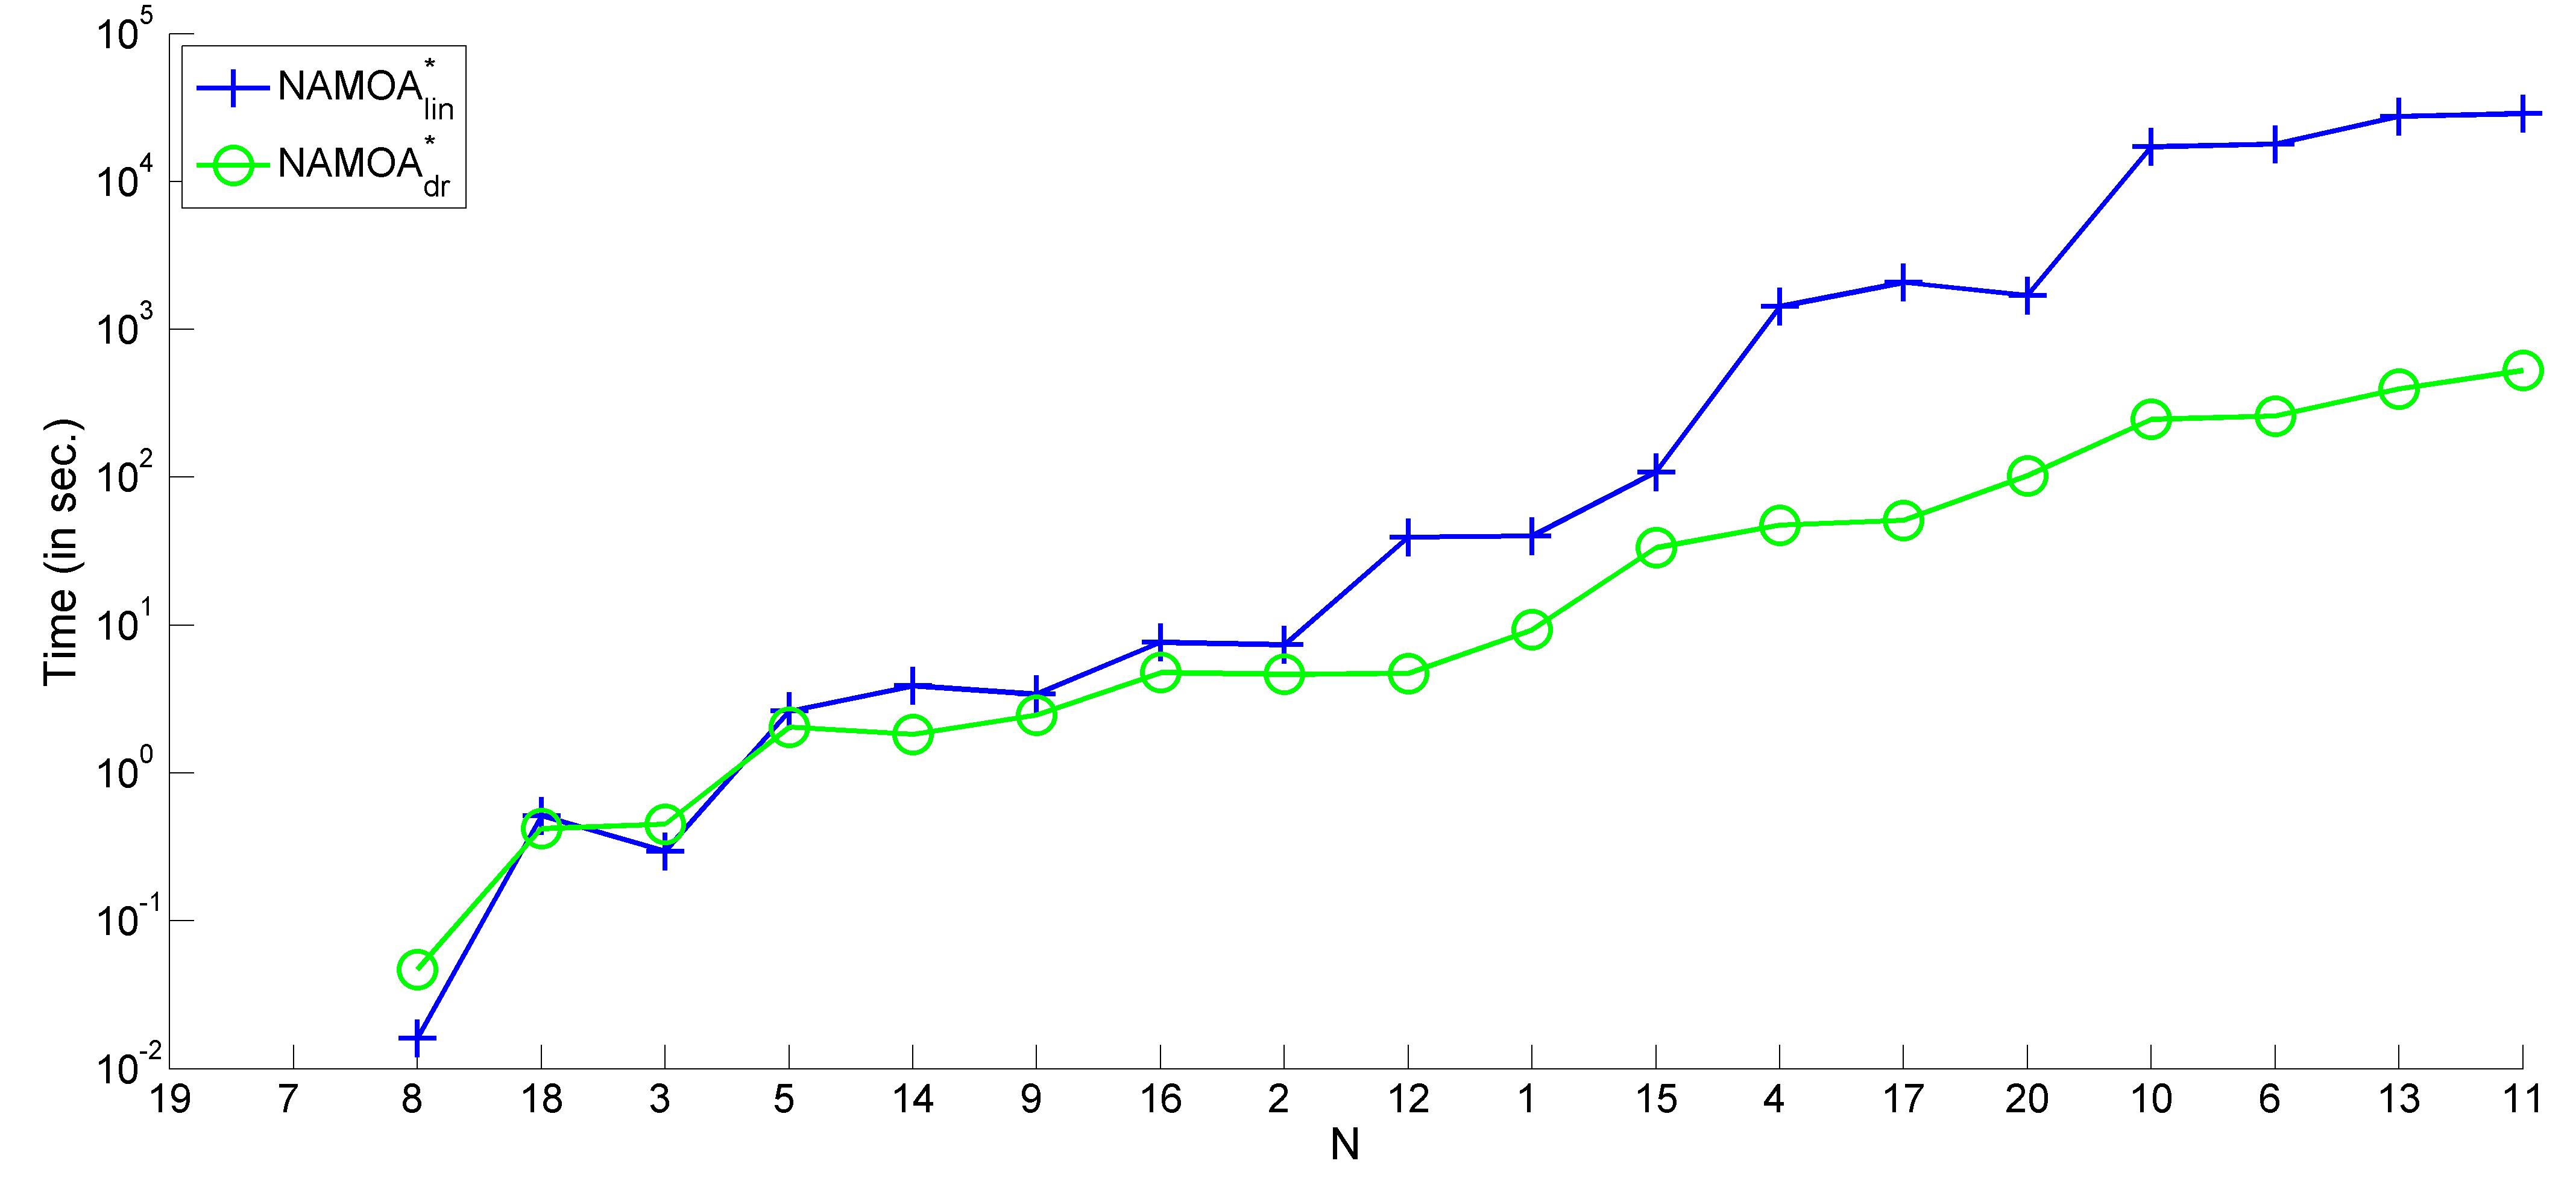
\includegraphics[width=1\textwidth]{Images/Chapter7/exe-times-VTcut}
\caption{Runtimes of \namoalin \ and \namoate \ for the VT$_{cut}$ map problems sorted by the number of labels expanded.}
\label{fig:7-3}
\end{figure}

Finally, Figures \ref{fig:7-4a} and \ref{fig:7-4b} show the percentage of labels filtered, pruned by open, and pruned by closed node labels over the total number of discarded labels by \namoate, for the maps of NY city and Vermont, respectively. The $X$-axis shows problem ids sorted by the number of scanned labels.

\begin{figure}
    \begin{center}
%
      \subfigure[NY city map]{%
            \label{fig:7-4a}
        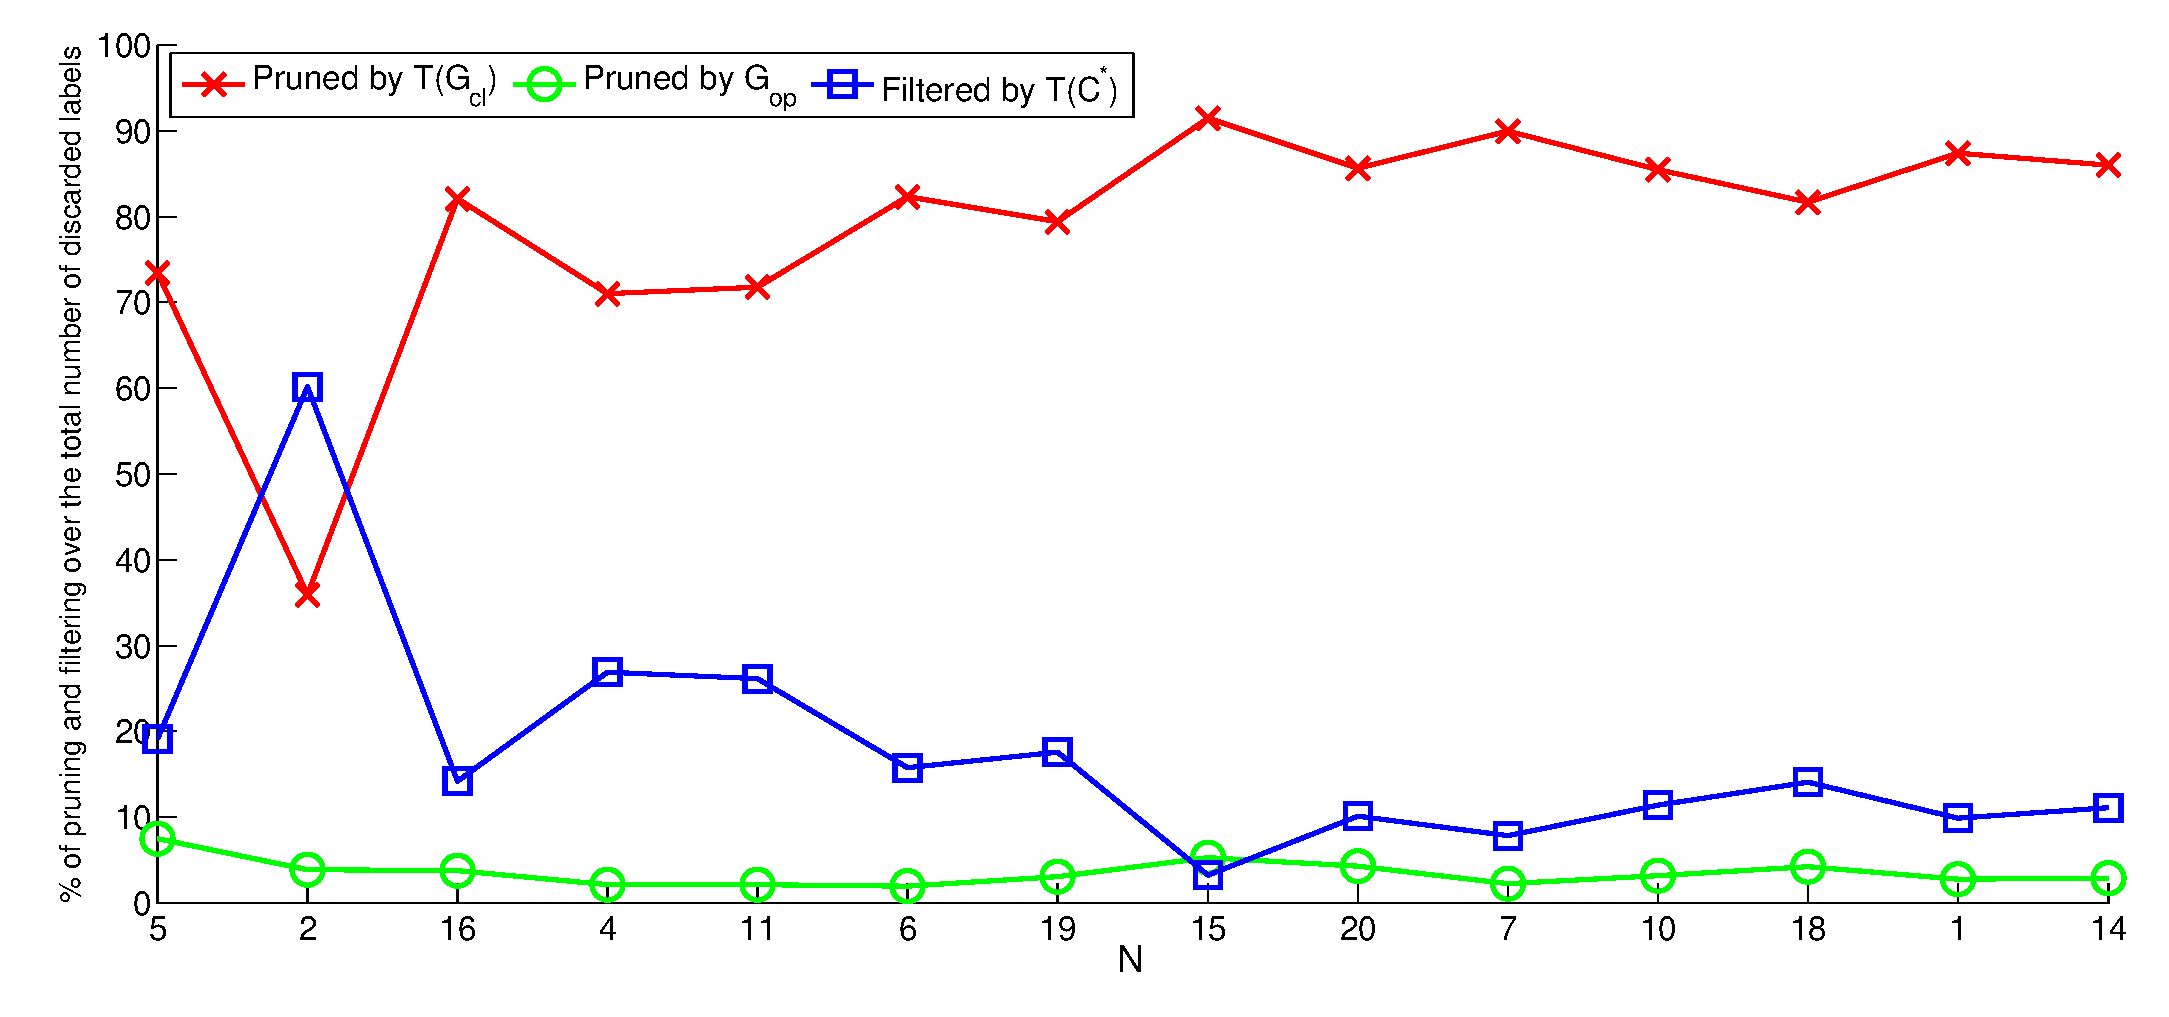
\includegraphics[width=0.95\textwidth]{Images/Chapter7/pruned-filtered-labels-dimacs-perc-NY}
        }\\ %  ------- End of the first row ----------------------%
      \subfigure[Vermont state map]{%
       		\label{fig:7-4b}  
 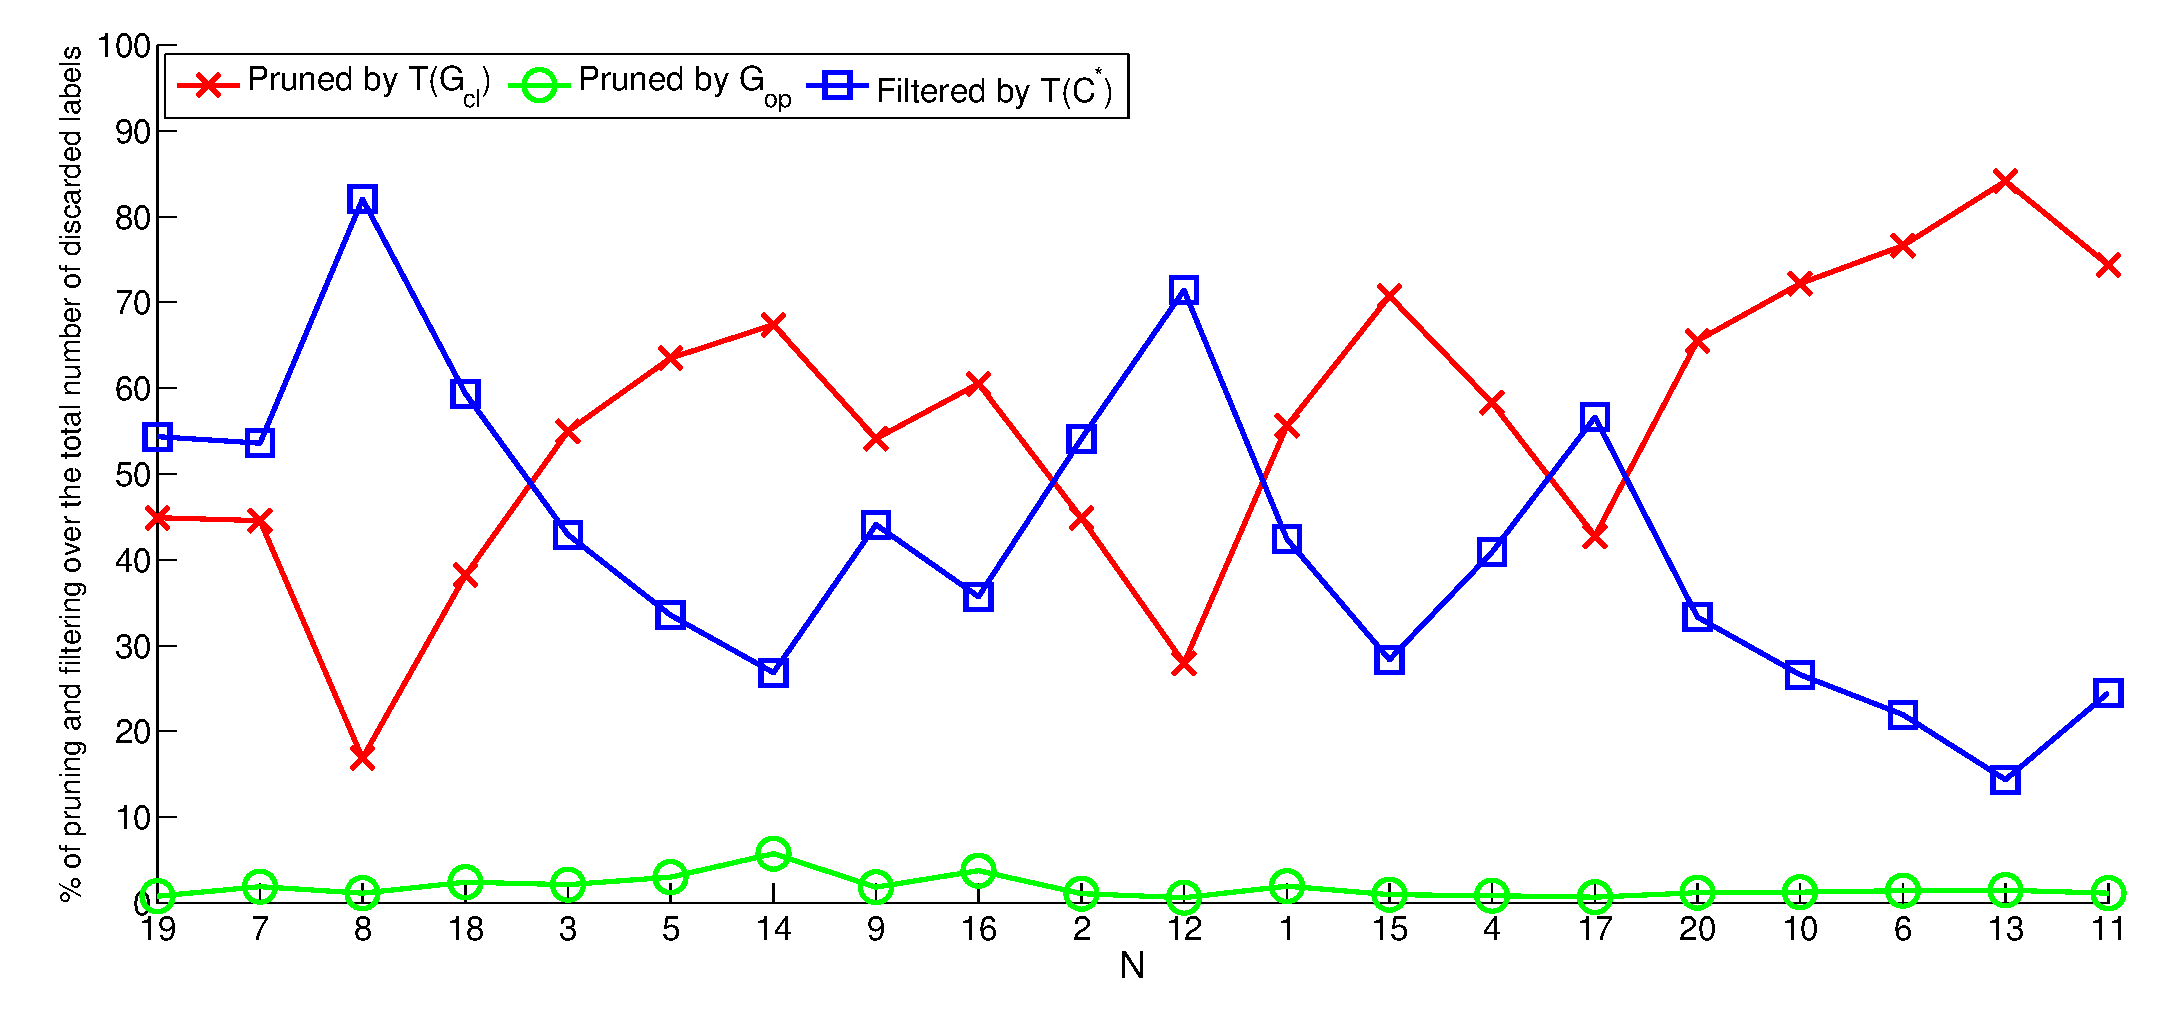
\includegraphics[width=0.95\textwidth]{Images/Chapter7/pruned-filtered-labels-dimacs-perc-VTcut}
        }\\ %  ------- End of the first row ----------------------%
    \end{center}
    \vspace{-0.25in} 
    \caption{%
Percentage of pruned and filtered labels over the total number of discarded labels by \namoate \ per solution depth in road map experiments.  
    }%
    \label{fig:7-4}

\end{figure}

The experiments on the realistic road map problems are much harder than the random grid problems. The largest solvable one (NY\#14) requiring up to 278 million label expansions (the deepest grid problems involved in average 2.5 million label expansions, and 3.3 million in the worst case). Again, \namoate \ clearly outperformed \namoalin, which could only solve problems involving less than 10.1 million label expansions (VT\#11). For such a problem, \namoate \ required only 1.83\% of the time needed by \namoalin. 

On one hand, \namoalin \ was capable of solving within the time limit only 4 problems from the NY set (20\%), while \namoate \ solved 14 (70\%) (see Table \ref{tab:7-13}), and on the other hand, in the test set of VT$_{cut}$ map, which was entirely solved by both algorithms, \namoate \ requires 1.74\% of the time needed by \namoalin (see Table \ref{tab:7-14}). Notice that for the NY map the algorithms were not capable of solving several problem instances in the given 8 hour time limit. These are indicated by symbol ``-'' in the table. Problems \#11 and \#6 were solved by \namoalin \ without time limit in 31 hours and 25 days, respectively.

Except for the simpler problems, cl-pruning was responsible for around 70 to 80\% of the discarded labels (see Figures \ref{fig:7-4a} and \ref{fig:7-4b}). In general, the ratio of filtered labels was larger than those discarded by op-pruning. Once again, this explains the efficiency achieved by t-discarding. Tables \ref{tab:7-12} and \ref{tab:7-13} show dramatic reductions in the sizes of the sets used for cl-pruning and filtering. For the hardest solved instance (NY\#14), the size of $T(\text{C}^*)$ is just $0.32\%$ the size of $\text{C}^*$. For the sets of closed labels, the ratio is $2.26\%$.

\begin{table}
\caption{Summary of $VT_{cut}$ map results.}
\label{tab:7-14}
\begin{center}
\begin{tabular}{ccccccc}
\hline \noalign{\smallskip}
Map & $(\frac{\sum G_{cl}}{\sum T(G_{cl})})$\% & $(\frac{\sum C^*}{\sum T(C^*)})$\% & $C^*$ & $t_{\text{NAMOA}^* \text{lin}}$ & $t_{\text{NAMOA}^* \text{dr}}$ & \% \\
\noalign{\smallskip} \hline 
%NY(2) & 4.56 & 2.25 & 2,164.1 & 2,988.1 & 132.2 & 4.42 \\
VT$_{cut}$ & 3.43 & 2.45 & 3,334.6 & 4,838.4 & 84.6 & 1.74 \\
%DE & 57.76 & 34.61 & 93 & 1.34 & 1.16 & 86.56 \\
\hline
\end{tabular} 
\end{center}
\end{table}

%-------------------------------------------------------------------
\subsection{Summary}
\label{chapEmpiricalAnalysis:subsec:summarydimacsnamoate}
%-------------------------------------------------------------------

The proposed t-discarding procedure proves to be very effective, reducing the time requirements over an order of magnitude over the most efficient search with the standard dominance checks. The new technique effectively extends the size of the three-objective problems that can be practically solved and opens a range of possibilities for multiobjective search algorithms to become more time-efficient. Thus, we then analyze the runtime performance of the application of this technique to the algorithm \lexgo.

%-------------------------------------------------------------------
\section{\texorpdfstring{\lexgote}{LEXGO*dr} \ vs \texorpdfstring{\lexgo}{LEXGO*}}
\label{chapEmpiricalAnalysis:sec:resultsdimacslexgote}
%-------------------------------------------------------------------

This section analyzes the three versions of \lexgo \ already presented, \lexgolex, \lexgolin, and \lexgote. A detailed description of \lexgo \ and \lexgote \ are presented in Sections \ref{chapMultiObjAlg:subsec:lexgo} and \ref{chapMultiObjAlg:subsec:lexgote}, respectively. 

The experiments below analyze the impact of the dimensionality reduction technique over the sets of random road map problems previously used, employing the goals already described in previous sections. The analysis is conducted over the Vermont problems and the NY city problems able to be solved by \lexgolex \ or \lexgolin. Notice that for a problem to be considered solved, all class I and II experiments must be solved within the time limit. The standard versions of \lexgo \ solved four and \lexgote \ six out of the twenty problems considered in the NY city map. 

%-------------------------------------------------------------------
\subsection{Analysis on class I experiments}
\label{chapEmpiricalAnalysis:subsec:analysisdimacslexgotec1}
%-------------------------------------------------------------------

Table \ref{tab:7-15} displays all the runtimes in seconds corresponding to Vermont and NY city problems solved by \lexgote. Table \ref{tab:7-16} summarizes the average execution times of Vermont problems for \lexgolex, \lexgolin, and \lexgote. Finally, Table \ref{tab:7-17} shows the runtimes of \lexgolex, \lexgolin, and \lexgote \ for problems NY\#4 and NY\#16 (runtimes of problems NY\#2 and NY\#5 are not shown since they are too small to be significative). 

In this first class of problems, \lexgote \ has a substantial advantage over both standard versions of \lexgo. \lexgote \ solves the full set of Vermont problems in 1.87\% and 2.01\% of the time needed by \lexgolex \ and \lexgolin \ when $k_1 = 1$, respectively. The time needed by \lexgote \ is 2.21\% and 2.39\%, and 3.91\% and 4.45\% with respect to \lexgolex \ and \lexgolin \ when $k_1 = 0.75$ and $k_1 = 0.5$. Regarding the experiments where the goals cannot be satisfied, the improvement of \lexgote \ is 11.45\% and 23.55\% over \lexgolex \ and \lexgolin \ when $k_1 = 0.25$, respectively, whereas all the runtimes when $k_1 = 0$ are equal to 0.03 seconds. It is also worth noting that the runtime of \lexgote \ when $k_1 = 0.25$ is greater than the runtimes when goals can be satisfied, i.e. when $k_1 = \{1, 0.75, 0.5\}$. This is due to the fact that the t-discarding technique is only applied to \lexgo \ when goals can be satisfied, hence, few problems when $k_1 = 0.25$ can benefit from the dimensionality reduction technique.

Let's turn now our attention to the NY city problems. Regarding problem NY\#4, \lexgote \ is more than twenty times faster than \lexgolex \ and \lexgolin \ when $k_1=\{1, 0.75\}$, sixteen times faster when $k_1=0.5$, and it has a similar performance when goals cannot be satisfied, i.e. when $k_1=\{0.25, 0\}$. 

\begin{table}
\caption{Class I experiments in road maps, runtimes in seconds of \lexgote \ for the experiments over Vermont and NY city maps.}
\label{tab:7-15}
\centering
\begin{tabular}{crrrrrrrr}
\hline \noalign{\smallskip}
& & \multicolumn{4}{c}{\lexgote} \\
\noalign{\smallskip} \cline{3-7} \noalign{\smallskip}
& $n$ & 1 & 0.75 & 0.5 & 0.25 & 0 & \multicolumn{1}{c}{$k_1$}\\
\noalign{\smallskip} 
\cline{1-8} \noalign{\smallskip} 
\parbox[t]{2mm}{\multirow{20}{*}{\rotatebox[origin=c]{90}{Vermont}}} &
1 & 9.68 & 4.71 & 1.35 & 0.45 & <0.01 \\
& 2 & 4.99 & 2.49 & 2.44 & 1.29 & 0.06 \\
& 3 & 0.68 & 0.42 & 0.20 & 0.18 & 0.03 \\
& 4 & 55.58 & 43.72 & 18.42 & 4.10 & 0.03 \\
& 5 & 2.37 & 1.82 & 0.59 & 0.06 & 0.04 \\
& 6 & 291.90 & 278.64 & 175.31 & 32.85 & 0.03 \\
& 7 & <0.01 & <0.01 & <0.01 & <0.01 & <0.01 \\
& 8 & 0.03 & <0.01 & <0.01 & <0.01 & <0.01 \\
& 9 & 3.16 & 2.15 & 1.37 & 0.60 & <0.01 \\
& 10 & 265.2 & 258.7 & 117.81 & 274.95 & 0.10 \\
& 11 & 584.45 & 427.56 & 401.99 & 357.66 & 0.09 \\
& 12 & 5.50 & 1.96 & 0.60 & 0.18 & 0.03 \\
& 13 & 464.60 & 491.77 & 332.82 & 2413.64 & 0.06 \\
& 14 & 2.10 & 1.87 & 0.95 & 0.10 & <0.01 \\
& 15 & 33.36 & 30.60 & 23.35 & 1.32 & 0.09 \\
& 16 & 4.52 & 1.90 & 1.70 & 0.88 & <0.01 \\
& 17 & 61.37 & 43.24 & 14.90 & 9.26 & 0.07 \\
& 18 & 0.37 & 0.24 & 0.32 & 0.07 & <0.01 \\
& 19 & <0.01 & <0.01 & <0.01 & <0.01 & <0.01 \\
& 20 & 108.15 & 80.15 & 53.52 & 43.00 & 0.03 \\
\noalign{\medskip}
\parbox[t]{2mm}{\multirow{6}{*}{\rotatebox[origin=c]{90}{NY city}}} &
2 & 0.87 & 0.65 & 0.28 & 0.01 & <0.01 \\
& 4 & 201.64 & 198.18 & 176.04 & 63.94 & 0.03 \\
& 5 & <0.01 & <0.01 & <0.01 & <0.01 & <0.01  \\
& 11 & 1,753.57 & 1,668.50 & 1,366.86 & 3,664.96 & 0.07 \\
& 16 & 118.63 & 116.22 & 62.97 & 0.96 & 0.01 \\
& 19 & 10,873.42 & 10,960.56 & 10,005.21 & 1,506.29 & 0.45 \\
\hline
\end{tabular}
\end{table}

\begin{table}
\caption{Class I experiments in road maps, summary of Vermont problems runtimes in seconds of \lexgolex, \lexgolin \ and \lexgote.}
\label{tab:7-16}
\centering
\begin{tabular}{rrrrrrrr}
\hline \noalign{\smallskip}
 & 1 & 0.75 & 0.5 & 0.25 & 0 & \multicolumn{1}{c}{$k_1$}\\
\noalign{\smallskip} 
\cline{2-6} \noalign{\smallskip} 
\lexgolex & 5,068.00 & 3,769.51 & 1,467.00 & 177.33 & 0.03 \\
\lexgolin & 4,716.90 & 3,497.26 & 1,287.37 & 205.39 & 0.03 \\
\lexgote & 94.90 &	83.59 & 57.38 & 157.02 & 0.03 \\
\hline
\end{tabular}
\end{table}


\begin{table}
\caption{Class I experiments in road maps, runtimes of \lexgolex, \lexgolin, and \lexgote \ for two NY city problems.}
\label{tab:7-17}
\centering
\scalebox{0.92}{
\begin{tabular}{lrrrrrr}
\hline %\noalign{\smallskip}
Problem & \multicolumn{3}{c} 4 & \multicolumn{3}{c}{16} \\
%\noalign{\smallskip} 
\hline
Algorithm & \lexgolex & \lexgolin & \lexgote & \lexgolex & \lexgolin & \lexgote \\
$(k_1=1)$    & 4,845.19 & 4,379.98 & 201.64 & 458.64 & 508.23 & 118.63 \\ 
$(k_1=0.75)$ & 4,038.80 & 4,184.89 & 198.18 & 234.34 & 370.87 & 116.22 \\ 
$(k_1=0.5)$  & 2,829.04   & 3,407.90 & 176.04  & 63.26  & 78.54 & 62.97\\ 
$(k_1=0.25)$ & 74.89   &  172.52 & 63.94 & 1.03    & 1.01 & 0.96 \\ 
$(k_1=0)$    & 0.01   &   0.03 & 0.03 & 0.01  & 0.01 & 0.01\\ 
\hline
\end{tabular}
}
\end{table}

%-------------------------------------------------------------------
\subsection{Analysis on class II experiments}
\label{chapEmpiricalAnalysis:subsec:analysisdimacslexgotec2}
%-------------------------------------------------------------------

Regarding the class II experiments, Table \ref{tab:7-18} displays all the runtimes in seconds corresponding to Vermont and NY city problems solved by \lexgote. The average runtimes of Vermont problems for \lexgolex, \lexgolin, and \lexgote \ are summarized in Table \ref{tab:7-19}. 

In these experiments, \lexgote \ also outperforms \lexgolex \ and \lexgolin. The relative advantage of \lexgote \ over \lexgolex \ and \lexgolin \ grows when the number of goal-optimal solution vectors is greater, as well as with the size of the problem. Thus, the time needed by \lexgote \ to solve the full set of Vermont problems is 41.87\% of the time needed by \lexgolex \ when $k_1 = 0.5$ and $k_2 = 0.125$. This comparative advantage grows to its maximum when $k_1 = k_2 = 0.75$, where \lexgote \ runtime is 2.21\% of \lexgolex \ runtime, i.e. \lexgote \ is more than 45 times faster than \lexgolex.

Table \ref{tab:7-20} shows a comparative of \lexgolex, \lexgolin, and \lexgote \ runtimes for problems NY\#4 and NY\#16. Problem NY\#16 does not show an apparent improvement when using \lexgote \ in many cases, since those cases cannot satisfy the provided goals. 

\begin{table}
\caption{Class II experiments in road maps, runtimes in seconds of \lexgote \ for the experiments over Vermont and NY city maps.}
\label{tab:7-18}
\centering
\scalebox{.78}{
\begin{tabular}{crrrrrrrrrrr}
\hline \noalign{\smallskip}
& & & \multicolumn{8}{c}{\lexgote} & \\
\noalign{\smallskip} \cline{3-10}
& & \multicolumn{4}{c|}{0.75} & \multicolumn{4}{c}{0.5} & \multicolumn{1}{c}{$k_1$}\\
& $n$  & 0.75 & 0.5625 & 0.375 & \multicolumn{1}{c|}{0.1875} & 0.5 & 0.375 & 0.25 & 0.125 & \multicolumn{1}{c}{$k_2$}\\
\noalign{\smallskip} 
\cline{1-11} \noalign{\smallskip} 
\parbox[t]{2mm}{\multirow{20}{*}{\rotatebox[origin=c]{90}{Vermont}}} &
1 & 4.71 & 4.71 & 6.32 & 13.90 & 1.36 & 1.42 & 1.78 & 2.20 \\ 
& 2 & 2.50 & 3.01 & 2.61 & 2.28 & 2.45 & 2.06 & 1.90 & 1.17 \\ 
& 3 & 0.42 & 0.64 & 0.38 & 0.20 & 0.20 & 0.20 & 0.13 & 0.11 \\ 
& 4 & 43.73 & 46.94 & 31.79 & 22.11 & 18.42 & 8.66 & 2.98 & 5.18 \\ 
& 5 & 1.83 & 1.47 & 0.91 & 0.70 & 0.59 & 0.30 & 0.34 & 0.53 \\ 
& 6 & 278.65 & 266.84 & 184.47 & 58.47 & 175.31 & 211.48 & 93.07 & 281.11 \\ 
& 7 & <0.01 & <0.01 & <0.01 & <0.01 & <0.01 & <0.01 & <0.01 & <0.01 \\ 
& 8 & <0.01 & <0.01 & <0.01 & <0.01 & <0.01 & <0.01 & <0.01 & <0.01 \\ 
& 9 & 2.15 & 1.92 & 1.56 & 1.00 & 1.37 & 0.91 & 0.78 & 0.61 \\ 
& 10 & 258.79 & 200.35 & 134.57 & 26.68 & 117.81 & 81.26 & 57.49 & 146.35 \\ 
& 11 & 427.57 & 418.82 & 394.06 & 264.59 & 402.00 & 395.54 & 313.09 & 209.03 \\ 
& 12 & 1.97 & 1.92 & 1.78 & 0.90 & 0.67 & 0.45 & 0.64 & 0.45 \\ 
& 13 & 491.78 & 450.97 & 438.63 & 144.61 & 332.83 & 304.70 & 189.07 & 17.80 \\ 
& 14 & 1.87 & 1.53 & 1.00 & 0.31 & 0.95 & 0.47 & 0.08 & 0.08 \\ 
& 15 & 30.61 & 28.50 & 24.96 & 26.46 & 23.35 & 22.56 & 22.51 & 15.85 \\ 
& 16 & 1.95 & 2.12 & 2.65 & 2.14 & 1.70 & 1.73 & 1.54 & 1.79 \\ 
& 17 & 43.24 & 43.51 & 35.51 & 25.83 & 14.93 & 10.09 & 1.42 & 1.64 \\ 
& 18 & 0.25 & 0.23 & 0.22 & 0.39 & 0.33 & 0.17 & 0.17 & 0.17 \\ 
& 19 & <0.01 & <0.01 & <0.01 & <0.01 & <0.01 & <0.01 & <0.01 & <0.01 \\ 
& 20 & 80.15 & 92.57 & 84.66 & 97.33 & 53.52 & 36.50 & 31.65 & 38.94 \\ 
\noalign{\medskip}
\parbox[t]{2mm}{\multirow{6}{*}{\rotatebox[origin=c]{90}{NY city}}} &
2 & 0.65 & 0.60 & 0.42 & 0.15 & 0.28 & 0.23 & 0.25 & 0.25 \\
& 4 & 198.18 & 220.77 & 225.99 & 128.49 & 176.04 & 177.32 & 170.47 & 35.67 \\
& 5 & <0.01 & - & - & - & - & - & - & - \\
& 11 & 1,668.50 & 1,617.41 & 2,653.90 & 2,852.52 & 1,366.86 & 1,860.42 & 2,727.67 & 4,532.50 \\
& 16 & 116.22 & 86.22 & 31.18 & 12.69 & 62.97 & 77.39 & 86.87 & 84.35 \\
& 19 & 10,960.56 & 15,407.65 & 20,771.40 & 5,270.44 & 10,005.21 & 12,456.02 & 5,141.12 & 4,519.28 \\
\hline
\end{tabular}
}
\end{table} 

\begin{table}
\caption{Class II experiments in road maps, runtimes in seconds of \lexgote \ for the experiments over Vermont and NY city maps.}
\label{tab:7-19}
\centering
\scalebox{.85}{
\begin{tabular}{rrrrrrrrrr}
\hline \noalign{\smallskip}
\multicolumn{1}{c}{} & \multicolumn{4}{c|}{0.75} & \multicolumn{4}{c}{0.5} & \multicolumn{1}{c}{$k_1$}\\
 & 0.75 & 0.5625 & 0.375 & \multicolumn{1}{c|}{0.1875} & 0.5 & 0.375 & 0.25 & 0.125 & \multicolumn{1}{c}{$k_2$}\\
\noalign{\smallskip} 
\cline{2-9} \noalign{\smallskip}
\lexgolex & 3,769.51 & 3,092.73 & 1,729.26 & 371.33 & 1,467.00 & 980.69 & 479.92 & 86.32 \\
\lexgolin & 3,497.26 & 2,782.82 & 1,781.04 & 424.25 & 1,287.37 & 977.48 & 499.61 & 109.20 \\
\lexgote & 83.59 & 78.30 & 67.31 & 34.40 & 57.39 & 53.93 & 35.93 & 36.15 \\
\hline
\end{tabular}
}
\end{table} 

\begin{table}
\caption{Class II experiments in road maps, runtimes in seconds of \lexgolex, \lexgolin, and \lexgote \ for two NY city problems.}
\label{tab:7-20}
\centering
\scalebox{0.9}{
\begin{tabular}{lrrrrrr}
\hline 
%\noalign{\smallskip}
Problem & \multicolumn{3}{c} 4 & \multicolumn{3}{c}{16} \\
%\noalign{\smallskip} 
\hline
Algorithm & \lexgolex & \lexgolin & \lexgote & \lexgolex & \lexgolin & \lexgote \\
$(0.75, \ 0.75)$ & 4,038.8 & 4,184.9 & 198.1 & 234.3 & 370.8 & 116.2 \\
$(0.75, \ 0.5625)$ & 4,060.7 & 4,229.3 & 220.7 & 121.9 & 219.9 & 86.2\\
$(0.75, \ 0.375)$ & 2,622.8 & 4,222.0 & 226.0 & 33.1 & 55.9 & 31.1\\
$(0.75, \ 0.1875)$ & 267.1 & 762.3 & 128.5 & 12.6 & 15.1 & 12.7\\
\noalign{\smallskip}
$(0.5. \ 0.5)$ & 2,829.0 & 3,407.9 & 176.0 & 63.2 & 78.5 & 62.9\\
$(0.5. \ 0.375)$ & 1,894.2 & 2,819.4 & 177.3 & 77.8 & 88.9 & 77.3\\
$(0.5. \ 0.25)$ & 627.1 & 1,757.5 & 170.5 & 84.3 & 92.9 & 86.8\\
$(0.5. \ 0.125)$ & 41.0 & 148.0 & 35.6 & 85.6 & 96.0 & 84.3\\  
\hline
\end{tabular}
}
\end{table}

%-------------------------------------------------------------------
\subsection{Summary}
\label{chapEmpiricalAnalysis:subsec:summarydimacslexgote}
%-------------------------------------------------------------------

In a similar manner as \lexgote \ outperforms \lexgo \ in random grids, the results do not change for road map problems. A greater speed-up can be observed in these experiments. When a large number of goal-optimal solution vectors from the Pareto frontier satisfy the goals, the t-discarding method is applied to a greater extent to \lexgote \ and speeds up the performance to up to 50 times faster than any previous version of \lexgo. Since this advantage grows with difficulty, the obtained results point out that \lexgote \ must be chosen over \lexgo \ in problems with a certain level of difficulty and satisfiable goals, although when goals cannot be satisfied \lexgote \ does only contribute with a slight advantage. 

%-------------------------------------------------------------------
\section{\texorpdfstring{\lexgote}{LEXGO*dr} \ vs \texorpdfstring{\namoate}{NAMOA*dr}}
\label{chapEmpiricalAnalysis:sec:resultsdimacste}
%-------------------------------------------------------------------

This section considers \namoate \ and \lexgote, versions of \namoa \ and \lexgo \ that employ the t-discarding technique described in Section \ref{chapMultiObjAlg:sec:Time-efficient-MSalg}. Since t-discarding can only be applied to \lexgo \ when goals can be satisfied, the question of its comparative performance to \namoate \ also arises for the road map problems. 

\namoate \ has been empirically proved to be more efficient than \namoa. In the same manner, \lexgote \ outperforms \lexgo. \namoate \ obtains a greater ratio of improvement over the standard versions of \namoa \ than \lexgote \ achieves over their counterparts of \lexgo. Thus, a final comparative analysis for random map problems between \namoate \ and \lexgote \ is presented in this section.  

The experiments are applied to the road map problems previously used. The goals employed to define the set of goal-optimal solution vectors are defined analogously as in Section \ref{chapEmpiricalAnalysis:sec:grids}. The analysis is conducted over the Vermont problems and the NY city problems able to be solved by \lexgote \ and \namoate, which were six and fourteen out of twenty, respectively.

%-------------------------------------------------------------------
\subsection{Analysis on class I experiments}
\label{chapEmpiricalAnalysis:subsec:analysisdimacstec1}
%-------------------------------------------------------------------

In Table \ref{tab:7-21} the results of \namoate \ and \lexgote \ are presented. Cases where \lexgote \ runtimes are faster than runtimes of \namoate \ are highlighted in bold. The average runtimes of the full set of Vermont map experiments are shown in Table \ref{tab:7-22}.

An expected overhead in \lexgote \ over \namoate \ is found when $k_1 = 1$. In this case, the overhead corresponding to the extra deviation pruning and filtering efforts represents 12.08\% of the runtime of \namoate. \lexgote \ shows a very similar runtime in average when $k_1 = 0.75$, only 1.26\% faster. When $k_1 = 0.5$, \lexgote \ clearly outperforms \namoate, being 32.22\% more efficient in runtime. As always, when the goals are located in the ideal point ($k_1 = 0$), \lexgote, with an average runtime of three hundredths of a second, outperforms \namoate.

A particular case of \lexgote \ can be observed in $k_1 = 0.25$ case. Problem VT\#13 is solved by \lexgote \ more than six times slower than by \namoate, and problem NY\#11 two and a half times slower. In order to understand this behavior we measured the percentage of times that a pruning operation is conducted in a time-efficient manner with respect to the total of pruning operations. We call this quotient $\eth$. Thus, $\eth_{13VT} = 0.4698$ and $\eth_{11NY} = 0.6938$ while other problems of similar difficulty, VT\#11 for example, present a much higher value ($\eth_{11} = 0.9531$). In other words, problem VT\#13 cannot use the Pareto pruning (dr) as often as the rest of the problems, in this case only 46.98\% of the times, and hence, its runtime is much higher than the average.

\begin{table}
\caption{Class I experiments in road maps, runtimes in seconds of \namoate \ and \lexgote \ for the experiments over Vermont and NY city maps.}
\label{tab:7-21}
\centering
\begin{tabular}{crrrrrrrrr}
\hline \noalign{\smallskip}
& & & \multicolumn{4}{c}{\lexgote} \\
\noalign{\smallskip} \cline{4-8} \noalign{\smallskip}
& $n$ & \namoate & 1 & 0.75 & 0.5 & 0.25 & 0 & \multicolumn{1}{c}{$k_1$}\\
\noalign{\smallskip} 
\cline{1-8} \noalign{\smallskip} 
\parbox[t]{2mm}{\multirow{20}{*}{\rotatebox[origin=c]{90}{Vermont}}} &
1 & \textbf{9.29} & 9.68 & \textbf{4.71} & \textbf{1.35} & \textbf{0.45} & \textbf{<0.01} \\
& 2 & \textbf{4.64} & 4.99 & \textbf{2.49} & \textbf{2.44} & \textbf{1.29} & \textbf{0.06} \\
& 3 & \textbf{0.45} & 0.68 & \textbf{0.42} & \textbf{0.20} & \textbf{0.18} & \textbf{0.03} \\
& 4 & \textbf{47.53} & 55.58 & \textbf{43.72} & \textbf{18.42} & \textbf{4.10} & \textbf{0.03} \\
& 5 & \textbf{2.04} & 2.37 & \textbf{1.82} & \textbf{0.59} & \textbf{0.06} & \textbf{0.04} \\
& 6 & \textbf{259.05} & 291.90 & 278.64 & \textbf{175.31} & \textbf{32.85} & \textbf{0.03} \\
& 7 & \textbf{<0.01} & \textbf{<0.01} & \textbf{<0.01} & \textbf{<0.01} & \textbf{<0.01} & \textbf{<0.01} \\
& 8 & \textbf{<0.01} & \textbf{<0.01} & \textbf{<0.01} & \textbf{<0.01} & \textbf{<0.01} & \textbf{<0.01} \\
& 9 & \textbf{2.46} & 3.16 & \textbf{2.15} & \textbf{1.37} & \textbf{0.60} & \textbf{<0.01} \\
& 10 & \textbf{246.09} & 265.20 & 258.70 & \textbf{117.81} & 274.95 & \textbf{0.10} \\
& 11 & \textbf{527.56} & 584.45 & \textbf{427.56} & \textbf{401.99} & \textbf{357.66} & \textbf{0.09} \\
& 12 & \textbf{4.71} & 5.50 & \textbf{1.96} & \textbf{0.60} & \textbf{0.18} & \textbf{0.03} \\
& 13 & \textbf{395.24} & 464.60 & 491.77 & \textbf{332.82} & 2,413.64 & \textbf{0.06} \\
& 14 & \textbf{1.82} & 2.10 & 1.87 & \textbf{0.95} & \textbf{0.10} & \textbf{<0.01} \\
& 15 & \textbf{33.35} & 33.36 & \textbf{30.60} & \textbf{23.35} & \textbf{1.32} & \textbf{0.09} \\
& 16 & \textbf{4.77} & \textbf{4.52} & \textbf{1.90} & \textbf{1.70} & \textbf{0.88} & \textbf{<0.01} \\
& 17 & \textbf{51.26} & 61.37 & \textbf{43.24} & \textbf{14.90} & \textbf{9.26} & \textbf{0.07} \\
& 18 & \textbf{0.42} & \textbf{0.37} & \textbf{0.24} & \textbf{0.32} & \textbf{0.07} & \textbf{<0.01} \\
& 19 & \textbf{<0.01} & \textbf{<0.01} & \textbf{<0.01} & \textbf{<0.01} & \textbf{<0.01} & \textbf{<0.01} \\
& 20 & \textbf{102.57} & 108.15 & \textbf{80.15} & \textbf{53.52} & \textbf{43.00} & \textbf{0.03} \\
\noalign{\medskip}
\parbox[t]{2mm}{\multirow{6}{*}{\rotatebox[origin=c]{90}{NY city}}} &
2 & \textbf{0.71} & 0.87 & \textbf{0.65} & \textbf{0.28} & \textbf{0.01} & \textbf{<0.01} \\
& 4 & \textbf{149.30} & 201.64 & 198.18 & 176.04 & \textbf{63.94} & \textbf{0.03} \\
& 5 & \textbf{<0.01} & \textbf{<0.01} & \textbf{<0.01} & \textbf{<0.01} & \textbf{<0.01} & \textbf{<0.01} \\
& 11 & \textbf{1,452.58} & 1,753.57 & 1,668.50 & \textbf{1,366.86} & 3,664.96 & \textbf{0.07} \\
& 16 & \textbf{106.89} & 118.63 & 116.22 & \textbf{62.97} & \textbf{0.96} & \textbf{0.01} \\
& 19 & \textbf{8,355.32} & 10,873.42 & 10,960.56 & 10,005.21 & \textbf{1,506.29} & \textbf{0.45} \\
\hline
\end{tabular}
\end{table}

\begin{table}
\caption{Class I experiments in road maps, average runtimes in seconds of \namoate \ and \lexgote \ for the set of Vermont map experiments.}
\label{tab:7-22}
\centering
\begin{tabular}{rrrrrrr}
\hline \noalign{\smallskip}
 & \multicolumn{5}{c}{\lexgote} \\
\noalign{\smallskip} \cline{2-6} \noalign{\smallskip}
\namoate & 1 & 0.75 & 0.5 & 0.25 & 0 & \multicolumn{1}{c}{$k_1$}\\
\noalign{\smallskip} 
\cline{1-6} \noalign{\smallskip} 
84.66 & 94.89 & 83.59 & 57.38 & 157.02 & 0.03 \\
\hline
\end{tabular}
\end{table}

%-------------------------------------------------------------------
\subsection{Analysis on class II experiments}
\label{chapEmpiricalAnalysis:subsec:analysisdimacstec2}
%-------------------------------------------------------------------

Regarding the second class of problems, unlike \lexgolex \ and \lexgolin \ with their \namoa \ counterparts, when applying the t-discarding technique to \lexgo \ and \namoa , \lexgote \ does not perform always faster than \namoate \ when $k_2$ values become stricter, in fact, the runtimes eventually increase notably although the number of label expansions decrease. This is due to the t-discarding method only applies to \lexgote \ when goals can be satisfied.

Table \ref{tab:7-23} displays the runtimes in seconds of \namoate \ and \lexgote \ for the Vermont and New York city maps experiments. Table \ref{tab:7-24} displays a summary of the average runtime of the full set of Vermont map experiments. On one hand, \lexgote \ outperforms in average \namoate \ in the Vermont map experiments, on the other hand, for the two most difficult problems solved by both algorithms, NY\#11 and NY\#19, \lexgote \ only runs faster than \namoate \ in three of the sixteen cases available. 

\begin{table}
\caption{Class II experiments in road maps, runtimes in seconds of \namoate \ and \lexgote \ for the experiments over Vermont and NY city maps.}
\label{tab:7-23}
\centering
\scalebox{.69}{
\begin{tabular}{crrrrrrrrrrrr}
\hline \noalign{\smallskip}
& & & \multicolumn{4}{c}{\lexgote} \\
\noalign{\smallskip} \cline{4-11} \noalign{\smallskip}
& & & \multicolumn{4}{c|}{0.75} & \multicolumn{4}{c}{0.5} & \multicolumn{1}{c}{$k_1$}\\
& $n$ & \namoate & 0.75 & 0.5625 & 0.375 & \multicolumn{1}{c|}{0.1875} & 0.5 & 0.375 & 0.25 & 0.125 & \multicolumn{1}{c}{$k_2$}\\
\noalign{\smallskip} 
\hline \noalign{\smallskip} 
\parbox[t]{2mm}{\multirow{20}{*}{\rotatebox[origin=c]{90}{Vermont}}} &
1 & \textbf{9.29} & \textbf{4.71} & \textbf{4.71} & \textbf{6.31} & 13.90 & \textbf{1.35} & \textbf{1.42} & \textbf{1.77} & \textbf{2.20}\\
& 2 & \textbf{4.64} & \textbf{2.49} & \textbf{3.01} & \textbf{2.60} & \textbf{2.27} & \textbf{2.44} & \textbf{2.05} & \textbf{1.90} & \textbf{1.17} \\
& 3 & \textbf{0.45} & \textbf{0.42} & 0.64 & \textbf{0.37} & \textbf{0.20} & \textbf{0.20} & \textbf{0.20} & \textbf{0.12} & \textbf{0.10} \\
& 4 & \textbf{47.53} & \textbf{43.72} & \textbf{46.94} & \textbf{31.79} & \textbf{22.10} &\textbf{18.42} & \textbf{8.65} & \textbf{2.97} & \textbf{5.17} \\
& 5 & \textbf{2.04} & \textbf{1.82} & \textbf{1.46} & \textbf{0.90} & \textbf{0.70} & \textbf{0.59} & \textbf{0.29} & \textbf{0.34} & \textbf{0.53} \\
& 6 & \textbf{259.05} & 278.64 & 266.84 & \textbf{184.47} & \textbf{58.46} & \textbf{175.31} & \textbf{211.47} & \textbf{93.07} & 281.11 \\
& 7 & \textbf{<0.01} & \textbf{<0.01} & \textbf{<0.01} & \textbf{<0.01} & \textbf{<0.01} & \textbf{<0.01} & \textbf{<0.01} & \textbf{<0.01} & \textbf{<0.01}\\
& 8 & \textbf{<0.01} & \textbf{<0.01} & \textbf{<0.01} & \textbf{<0.01} & \textbf{<0.01} & \textbf{<0.01} & \textbf{<0.01} & \textbf{<0.01} & \textbf{<0.01}\\
& 9 & \textbf{2.46} & \textbf{2.15} & \textbf{1.91} & \textbf{1.56} & \textbf{0.99} & \textbf{1.37} & \textbf{0.90} & \textbf{0.78} & \textbf{0.60} \\
& 10 & \textbf{246.09} & 258.70 & \textbf{200.35} & \textbf{134.56} & \textbf{26.67} & \textbf{117.81} & \textbf{81.26} & \textbf{57.48} & \textbf{146.34}  \\
& 11 & \textbf{527.56} & \textbf{427.56} & \textbf{418.81} & \textbf{394.05} & \textbf{264.59} & \textbf{401.99} & \textbf{395.54} & \textbf{313.09} & \textbf{209.02} \\
& 12 & \textbf{4.71} & \textbf{1.96} & \textbf{1.91} & \textbf{1.77} & \textbf{0.90} & \textbf{0.60} & \textbf{0.45} & \textbf{0.64} & \textbf{0.45} \\
& 13 & \textbf{395.24} & 491.77 & 450.96 & 438.62 & \textbf{144.61} & \textbf{332.82} & \textbf{304.70} & \textbf{189.07} & \textbf{17.80} \\
& 14 & \textbf{1.82} & 1.87 & \textbf{1.52} & \textbf{0.99} & \textbf{0.31} & \textbf{0.95} & \textbf{0.46} & \textbf{0.07} & \textbf{0.07} \\
& 15 & \textbf{33.35} & \textbf{30.60} & \textbf{28.50} & \textbf{24.96} & \textbf{26.45} & \textbf{23.35} & \textbf{22.55} & \textbf{22.51} & \textbf{15.84} \\
& 16 & \textbf{4.77} & \textbf{1.90} & \textbf{2.12} & \textbf{2.65} & \textbf{2.13} & \textbf{1.70} & \textbf{1.73} & \textbf{1.54} & \textbf{1.79} \\
& 17 & \textbf{51.26} & \textbf{43.24}  & \textbf{43.50} & \textbf{35.50} & \textbf{25.83} & \textbf{14.90} & \textbf{10.09} & \textbf{1.41} & \textbf{1.63} \\
& 18 & \textbf{0.42} & \textbf{0.24} & \textbf{0.23} & \textbf{0.21} & \textbf{0.39} & \textbf{0.32} & \textbf{0.17} & \textbf{0.17} & \textbf{0.17} \\
& 19 & \textbf{<0.01} & \textbf{<0.01} & \textbf{<0.01} & \textbf{<0.01} & \textbf{<0.01} & \textbf{<0.01} & \textbf{<0.01} & \textbf{<0.01} & \textbf{<0.01}\\
& 20 & \textbf{102.57} & \textbf{80.15} & \textbf{92.57} & \textbf{84.66} & \textbf{97.32} & \textbf{53.52} & \textbf{36.50} & \textbf{31.65} & \textbf{38.93} \\
\noalign{\medskip}
\parbox[t]{2mm}{\multirow{6}{*}{\rotatebox[origin=c]{90}{NY city}}} &
2 & \textbf{0.71} & \textbf{0.65} & \textbf{0.60} & \textbf{0.42} & \textbf{0.15} & \textbf{0.28} & \textbf{0.23} & \textbf{0.24} & \textbf{0.25} & \\
& 4 & \textbf{149.30} & 198.18 & 220.77 & 225.99 & \textbf{128.49} & 176.04 & 177.32 & 170.47 & \textbf{35.67} \\
& 5 & \textbf{<0.01} & \textbf{<0.01} & \textbf{<0.01} & \textbf{<0.01} & \textbf{<0.01} & \textbf{<0.01} & \textbf{<0.01} & \textbf{<0.01} & \textbf{<0.01} \\
& 11 & \textbf{1,452.58} & 1,668.50 & 1,617.41 & 2,653.90 & 2,852.52 & \textbf{1,366.86} & 1,860.42 & 2,727.67 & 4,532.50  \\
& 16 & \textbf{106.89} & 116.22 & \textbf{86.22} & \textbf{31.18} & \textbf{12.69} & \textbf{62.97} & \textbf{77.39} & \textbf{86.87} & \textbf{84.35} \\
& 19 & \textbf{8,355.32} & 10,960.56 & 15,407.65 & 20,771.40 & \textbf{5,270.44} & 10,005.21 & 12,456.02 & \textbf{5,141.12} & \textbf{4,519.28} \\
\hline
\end{tabular}
}
\end{table}

\begin{table}
\caption{Class II experiments in road maps, average runtimes in seconds of \namoate \ and \lexgote \ for the set of Vermont map experiments.}
\label{tab:7-24}
\centering
\begin{tabular}{rrrrrrrrrrr}
\hline \noalign{\smallskip}
 & \multicolumn{8}{c}{\lexgote} & \\
\noalign{\smallskip} \cline{2-9} \noalign{\smallskip}
& \multicolumn{4}{c|}{0.75} & \multicolumn{4}{c}{0.5} & \multicolumn{1}{c}{$k_1$}\\
\namoate & 0.75 & 0.5625 & 0.375 & \multicolumn{1}{c|}{0.1875} & 0.5 & 0.375 & 0.25 & 0.125 & \multicolumn{1}{c}{$k_2$}\\
\noalign{\smallskip} 
\hline \noalign{\smallskip} 
84.66 & 83.59 & 78.30 & 67.31 & 34.40 & 57.38 & 53.93 & 35.93 & 36.15 \\
\hline
\end{tabular}
\end{table}

%-------------------------------------------------------------------
\subsection{Summary}
\label{chapEmpiricalAnalysis:subsec:summarydimacste}
%-------------------------------------------------------------------

The results obtained for road map problems are significantly different from the experiments conducted on grid problems. \lexgote \ does not always perform faster than \namoate \ when goals cannot be satisfied, in fact, its runtime in problems with unsatisfiable goals can be significantly higher. In addition, \lexgote \ may perform slower when the number of expansions is reduced, due to the fact that the t-discarding method may not be applied to prune and filter new scanned labels. 

The average of the full set of Vermont problems gives \lexgote \ an advantage over \namoate \ for all the analyzed class II experiments and most of the class I experiments. \namoate \ outperforms \lexgote \ only when $k_1 = 1$ and $k_1 = 0.25$. The former case is obvious, since all goal-optimal solution vectors are also Pareto-optimal, therefore, \lexgote \ only introduces extra calculations to the process of returning the full Pareto set. The latter, it corresponds to an extreme case of bad performance of \lexgote. When $k_1 = 0.25$ and the difficulty of the problem grows, the impact of the regular pruning and filtering on the runtime highly affects \lexgote \ performance. Thus, we can also observe than \namoate \ was capable of solving 14 out of the 20 problems of New York city, while \lexgote \ solved only 6. This can only be attributed to the regular pruning and filtering operations, highly inefficient in time compared to t-discard alternatives.

%-------------------------------------------------------------------
\section{Summary on road map problems}
\label{chapEmpiricalAnalysis:sec:summarygridste}
%-------------------------------------------------------------------

The experiments previously presented are a new contribution to the multicriteria route planning. To the best of our knowledge, these are the largest problems solved with 3 objectives. 

The main contributions of this thesis are \lexgo, a new devised algorithm to cope with lexicographic goals on MSP, the t-discarding method, which applied to MSP achieves a significant runtime performance improvement, and the application of the t-discarding method to \namoa \ and \lexgo \ within a broader set of experiments that were previously reported in the literature. 

Previous results to the experiments shown in this thesis were reported in \citet{Pulido2015}. The experiments reported in this chapter go beyond those previously reported and add \lexgolin \ and \lexgote \ algorithms to the analyses. Furthermore, additional cases of \lexgo \ has been evaluated, for instance, $k_1=0.75$ in class II experiments. 

The empirical evaluation conducted in this chapter over realistic road map problems confirms the previous results over random grids to some extent.
\lexgo \ has been formally and empirically proved to be more efficient for the majority of the analyzed cases than \namoa, regardless the selection order and the road map. 

The t-discarding method applied to \namoa \ and \lexgo \ is also proved formally and now empirically to improve significantly the performance of these algorithms. Finally, the comparison between the best alternatives, \namoate \ and \lexgote, allow us to differentiate those cases where \lexgote \ may be chosen over \namoate. 

\begin{table}
\caption{Runtime comparison - summary table for road map experiments.}
\centering
\scalebox{0.92}{
\begin{tabular}{p{0.35\textwidth}p{0.65\textwidth}}
\hline \noalign{\smallskip}
Comparison & Results \\
\noalign{\smallskip} \hline
%& Class I & Class II \\
%\noalign{\smallskip} \hline
\textbf{\namoalin \ vs \namoalex} & In contrast to the experiment results of random grids, where \namoalin \ outperforms \namoalex \ by a factor of two, \namoalin \ has only a slight performance advantage on road maps. \\
\noalign{\smallskip}\hline
\noalign{\smallskip}
\textbf{\lexgolin \ vs \lexgolex} & In a slightly different way to the experiment results for random grids, \lexgolin \ also obtain better runtimes than \lexgolex, although the difference between them is significantly smaller on road maps. \\ 
\noalign{\smallskip}\hline
\noalign{\smallskip}
\textbf{\lexgo \ vs \namoa} & The selection order does not make a difference in the comparative performance between \lexgo \ and \namoa \ (in contrast to the experiment results for random grids). The speed-up of \lexgo \ over \namoa, however, remains outstanding for $k_1 \leq 0.5$, and its time overhead for $k_1 = \{0.75, 1\}$ is practically zero. \\
\noalign{\smallskip}\hline
\noalign{\smallskip}
\textbf{\namoate \ vs \namoa} & \namoate \ is almost two orders of magnitude faster than \namoalex \ and \namoalin \ for the most difficult problems. Moreover, \namoate \ extends the size of the three objective problems that can be solved in practice. \\
\noalign{\smallskip}\hline
\noalign{\smallskip}
\textbf{\lexgote \ vs \lexgo} & In a similar way to the results for random grids, \lexgote \ achieves speed-ups of up to 50 times faster than any version of \lexgo \ with standard discarding procedures and goals that can be satisfied. When goals can not be satisfied, \lexgote \ does have a slight advantage of performance. Its relative improvement also grows with problem difficulty. \\
\noalign{\smallskip}\hline
\noalign{\smallskip}
\textbf{\lexgote \ vs \namoate} & The comparative performance of \lexgote \ over \namoate \ is significantly different in road map problems than in random grids. \namoate \ outperforms \lexgote \ when $k_1 = 1$ and $k_1 = 0.25$. The latter corresponds to an extreme case of bad performance for \lexgo, since the standard pruning and filtering procedures highly impact the runtime performance. \lexgote \ outperforms \namoate \ in the rest of the cases, i.e. when $k_1 = \{0.75, 0.5, 0\}$ in class I experiments and all class II experiments. \\
\hline
\end{tabular}
}
\label{tab:7-25}
\end{table}


%---------------------------------------------------------------------
%
%                          Part Conclusions
%
%---------------------------------------------------------------------
%
% PartConclusions.tex
% Copyright 2015 Dr. Francisco J. Pulido
%
% This file belongs to the PhD titled "New Techniques and Algorithms for Multiobjective and Lexicographic Goal-Based Shortest Path Problems", distributed under the Creative Commons Licence Attribution-NonCommercial-NoDerivs 3.0, available in http://creativecommons.org/licenses/by-nc-nd/3.0/. The complete PhD dissertation is freely accessible from http://www.lcc.uma.es/~francis/
%
% This thesis has been written adapting the TeXiS template, a LaTeX template for writting thesis and other documents. The complete TeXiS package can be obtained from http://gaia.fdi.ucm.es/projects/texis/. TeXis is distributed under the same conditions of the LaTeX Project Public License (http://www.latex-project.org/lppl.txt). The complete license is available in http://creativecommons.org/licenses/by-sa/3.0/legalcode
%
%---------------------------------------------------------------------

\partTitle{Conclusions}

\partDesc{
The last part of this thesis gathers the conclusions of this research work.

Chapter \ref{ChapConclusions} sums up the conclusions collected from this research work into nine different points, deducted from the formal and empirical analyses conducted in the second part. Furthermore, some lines for future developments and improvements are also suggested.
}

\makepart

%---------------------------------------------------------------------
%
% Chapter 8: Conclusions and Future Work
%
%---------------------------------------------------------------------
%
% ChapConclusions.tex
% Copyright 2015 Dr. Francisco J. Pulido
%
% This file belongs to the PhD titled "New Techniques and Algorithms for Multiobjective and Lexicographic Goal-Based Shortest Path Problems", distributed under the Creative Commons Licence Attribution-NonCommercial-NoDerivs 3.0, available in http://creativecommons.org/licenses/by-nc-nd/3.0/. The complete PhD dissertation is freely accessible from http://www.lcc.uma.es/~francis/
%
% This thesis has been written adapting the TeXiS template, a LaTeX template for writting thesis and other documents. The complete TeXiS package can be obtained from http://gaia.fdi.ucm.es/projects/texis/. TeXis is distributed under the same conditions of the LaTeX Project Public License (http://www.latex-project.org/lppl.txt). The complete license is available in http://creativecommons.org/licenses/by-sa/3.0/legalcode
%
%---------------------------------------------------------------------

\chapter{Conclusions and Future Work}
\label{ChapConclusions}
%
\begin{FraseCelebre}
\begin{Frase}
Time is really the only capital that any human being has and the thing that he can least afford to waste or lose.
\end{Frase}
\begin{Fuente}
Thomas Edison (1847-1931)
\end{Fuente}
\end{FraseCelebre}
%
%\begin{resumen}
%...
%\end{resumen}

Multicriteria Decision Making (MCDM) is a branch of Operations Research that considers multiple criteria in decision-making environments. Goal Programming is a branch of MCDM that models preferences using goals, i.e. establishing target values over a set of attributes. The Multicriteria Search Problem (MSP) is the natural extension for the multiobjective case of the Shortest Path Problems, which are one of the most extensively studied problems in Artificial Intelligence and Operations Research. New developments in these fields are of practical importance in current research.

The main goals of this thesis are to analyze the use of goal-based preferences in Multicriteria Shortest Path Problems, and provide new techniques and algorithms framed in this field. In particular, we are concerned with exact techniques where the preferences of the decision maker (DM) are modeled into levels of pre-emptive importance. Within each level, one or more targets are defined as the expectations of the DM and weights characterize the importance of the criteria. 

In the literature, there is a general agreement that labeling multicriteria search algorithms are frequently the best choice to solve MSP \citep{skriverandersen2000,Raith2009,Raith2009a}. Moreover, two strategies can be used in these algorithms, node-selection and label-selection, and the latter has been repeatedly proved to be more efficient in label-setting algorithms \citep{Paixao2007,PerezdelaCruz2013}. Furthermore, the use of lower bound functions has been shown as a great advantage in the efficiency of these algorithms \citep{Mandow2010, Machuca2012a}. Thus, under the framework of lexicographic goal-based preferences we have analyzed two different strategies. The first one is to calculate the whole set of efficient solutions to the problem and extract the satisfactory solutions a posteriori. \namoa \ is included in these algorithms. The second one is to employ the goals given by the DM to bound the area of interesting solutions. The main goal of our new devised algorithm, \lexgo, which falls in this second category, is to achieve improvements over the efficiency of \namoa \ in the calculation of this set of efficient solutions according to the goals.

Time has been shown as the limiting factor in the performance of multicriteria search algorithms. The majority of the time effort is devoted to check dominance against set of labels and thereby discard new generated alternatives. Our new proposed dimensionality reduction technique, called t-discarding, speeds up the processes of pruning and filtering, which are responsible of discarding new paths by comparing to partial and full paths, respectively.  

The new dimensionality reduction technique can be used to improve the time requirements of labeling multicriteria search algorithms. In particular, we introduced \namoate \ and \lexgote \ as the versions of the algorithms previously analyzed that employ the dimensionality reduction technique. Finally, we perform extensive benchmarking to all the algorithms proposed over two scenarios, random grids and road maps problems. 

In summary, a new exact label-setting multicriteria search algorithm is proposed to deal with MSP with lexicographic goal-based preferences and improve the performance of the full search. In addition, a new technique to speed up the processes of discarding new alternatives is also proposed, as well as formally and practically applied. Finally, empirical analyses test all the algorithmic alternatives. 

%-------------------------------------------------------------------
\section{Conclusions}
\label{ChapConclusions:sec:conclusions}
%-------------------------------------------------------------------

The main conclusions of this doctoral dissertation can be enumerated as follows:

\begin{enumerate}

    \item \textbf{\lexgo, a new multicriteria search algorithm has been proposed.} Multiobjective search algorithms benefit from the principle of optimality, i.e. an optimal path is made up of optimal subpaths. Regrettably, this property does not hold for lexicographic goal-based preferences. We have introduced a new exact label-setting algorithm that returns the subset of Pareto-optimal paths that satisfy a set of lexicographic goals grouped in pre-emptive priority levels, or the subset that minimizes deviation from goals if these cannot be fully satisfied. Along with \lexgo, it has been proposed a specific pruning condition that allows to reduce the number of paths explored in goal-based search. We have also provided formal proofs on the correctness of the new pruning procedure and \lexgo.  

    \item \textbf{\lexgo \ is more efficient than a full Pareto search.} \lexgo \ is theoretically proved to expand a subset of the labels expanded by the full Pareto search. Since the number of expanded labels is not the only relevant factor in the analysis of multicriteria search algorithms, we compared \lexgo \ and \namoa \ over random grids and road maps problems. In both cases, a small time overhead can be observed for \lexgo \ when the full Pareto frontier satisfies the goals, and the relative performance of \lexgo \ over \namoa \ improves progressively whenever the set of efficient solutions is reduced. Elsewhere  in the test sets, \lexgo \ achieves important reductions in time requirements of about one order of magnitude when goals are satisfied for some Pareto solutions, and up to four orders of magnitude whenever goals can not be fully satisfied.  
    
    \item \textbf{The label selection policy has an important impact on time performance.} We have conducted experiments with two different label selection policies, lexicographic and linear aggregation, over \namoa \ and \lexgo. It can be observed that \namoalin \ is approximately 50\% faster than \namoalex / in random grids. The comparison between \lexgolex \ and \lexgolin \ is however, not that straightforward. \lexgolin \ is only faster than \lexgolex \ when a high percentage of the Pareto frontier is returned, and slower whenever a reduced number of solutions satisfy all goals. When goals cannot be satisfied, \lexgolex \ and \lexgolin \ show a very similar performance.
    
    \item \textbf{A new dimensionality reduction technique, t-discarding, is proposed.} Time rather than space is the limiting factor to increase the number of Multiobjective Search Problems that can be practically solved. Thus, we have devised a simple but very effective technique to decrease the number of labels belonging to the sets in charge of discarding new alternatives. This technique is applied under reasonable circumstances: when a consistent lower bound function is employed along with the algorithm and a lexicographic order is used to select alternatives from OPEN. 
    
    \item \textbf{t-discarding is extensively used to discard labels.} We employ sets of closed labels, $G_{cl}(n)$, and full solution paths, COSTS, to perform pruning (cl-pruning) and filtering processes, respectively. Nonetheless, sets of partial open labels, $G_{op}(n)$,  can not benefit from this technique to speed up dominance checks (op-pruning). Therefore, we launched experiments to measure the percentage of op-pruned, cl-pruned and filtered labels over the total number of discarded labels. Neither in the experiments over random grids nor in the experiments over road maps op-pruning was employed in more than 10\% of the cases. Then, we can ensure t-discarding is highly applied to discard new alternatives.
    
    \item \textbf{t-discarding checks dominance against reduced sets of labels.} Relative size of the sets of truncated labels over the original sets is theoretically unknown. However, in practice, an experimental evaluation was conducted and this size was around two orders of magnitude smaller for the difficult grid problems and about two to three orders for difficult road maps problems. Moreover, the relative advantage of t-discarding is incremented gradually with problem size, hence, this new contribution can effectively extends the set of Multicriteria Search Problems that can be practically solved.   
    
    \item \textbf{\namoate \ reduces \namoa \ time requirements.} The t-discarding technique can be applied to exact multicriteria search algorithms like \namoa. In random grid problems, the speed-up for the most difficult problems was 8.94 by \namoate \ over \namoalin, the fastest studied version of \namoa. In road maps problems, the speed-up for the most difficult problem solved by \namoalin \ was 26.55, i.e. \namoate \ solved the problem in 3.77\% of the time needed by \namoalin. \namoate \ also extended the number of solved problems from 4 out of 20 by \namoalin \ to 14 out of 20 in a very difficult set of realistic problems with three criteria.
    
    \item \textbf{\lexgote \ reduces standard \lexgo \ time requirements in some cases.} The t-discarding technique requires the lexicographical selection of evaluation vectors. This imposed lexicographic order in \lexgote \ makes those cases where the goals cannot be satisfied incompatible with the correctness of t-discarding. However, \lexgote \ can benefit from the use of t-discarding when goals can be satisfied, which indeed are the most difficult problems, and achieve speed-ups of up to 8.31 and 21.72 for the most difficult random grid and road map problems, respectively. 
    
    \item \textbf{A comparative between \namoate \ and \lexgote.} Finally, we have conducted an experimental evaluation of the most successful alternatives studied. In random grids, the inclusion of the t-discarding technique makes \namoate \ be the alternative to choose whenever goals can be satisfied, specially, when a higher percentage of the non-dominated solutions satisfy the goals. \lexgote \ is the best alternative whenever goals can not be fully satisfied or a smaller portion of the Pareto frontier is returned. 

In road maps problems, the results are compatible but significantly different. It must be pointed out that $k_1 = 0.25$ represents an extreme case of bad performance for \lexgote. Thus, in class I experiments, \namoate \ outperforms \lexgote \ when $k_1 = 1$ and $k_1 = 0.25$, and \lexgote \ has a better performance when $k_1 = \{0.75, 0.5, 0\}$. In class II experiments, the majority of \lexgote \ experiments perform faster than \namoate \ experiments. When goals could be satisfied there existed a significant number of problems that were solved by \namoate \ and could not be solved within the time limit by \lexgote.
      
\end{enumerate}

%-------------------------------------------------------------------
\section{Future Work}
\label{ChapConclusions:sec:futurework}
%-------------------------------------------------------------------

This doctoral dissertation has contributed new algorithms and techniques. These contributions have also raised new future lines of research where current developments can be effectively improved. The following lines may justify further investigation: 

\begin{itemize}

	\item The experimental evaluation conducted in this thesis has remarked the importance of the label selection policy for time performance. The determination of an optimal policy is a desirable issue for a deeper study.  
	
	\item The study and development of more efficient data structures to store the sets of open and closed labels, as well as the queue of alternatives, is a current research. All the algorithms presented in this thesis could benefit from more efficient implementations of these data structures.

	\item Two important formal analyses could be carried out regarding the optimality of \lexgo \ when used with consistent lower bounds. The first one, research the possibility that \lexgo \ is optimal in its class of exact goal-based algorithms according to the number of labels expanded. The second one, investigate theoretically the possibility that \lexgo \ expands an equal or smaller number of labels when using more informed lower bound functions.

	\item \lexgo \ can be extended to use other GP models or other formulas to measure the deviation from goals. New pruning and/or filtering rules will probably need to be developed for each particular case, in order to enhance their efficiency.
	
    \item Apply t-discarding to other multicriteria search algorithms with lower bounds. We have applied the t-discarding technique to \namoa, but it can be applied to a significant number of algorithms to reduce their time requirements.  
	
	\item Both \namoa \ and \lexgo \ return the set of all non-dominated (or goal-optimal for \lexgo) solutions. In difficult problems seek for the whole set of non-dominated solutions leads to high runtime requirements. However, there are other multicriteria techniques that seek only for a single efficient solution, as Compromise Search. Some of the conclusions reported here, like the performance of selection orders or the importance of dominance checks in runtime, can be useful to extend other multicriteria decision models.
	
	\item Multicriteria search in road maps is becoming more popular in the last few years. Since the query time for single-objective shortest path problems is in the order of microseconds, the natural evolution is the resolution of problems that involve more than one criterion. The advanced optimization techniques applied to the single-objective problem, like multilevel graphs \citep{schulzetal2002} or contraction hierarchies \citep{Geisberger2008} represent possibilities for multicriteria search which deserve further research. For instance, preprocessing techniques like contraction hierarchies would require a multicriteria bidirectional search. In fact, this is another field of research of the author \citep{Pulido2011,Pulido2012}, hence, its application is of his great interest.   

	\item Finally, a recurrent line of research is to identify new potential domains to apply multicriteria search, as well as the combination with other disciplines to approach MSP from a different perspective.

\end{itemize}	


% Ap�ndices
\appendix

%---------------------------------------------------------------------
%
%                          Part Appendix
%
%---------------------------------------------------------------------
%
% PartAppendix.tex
% Copyright 2015 Dr. Francisco J. Pulido
%
% This file belongs to the PhD titled "New Techniques and Algorithms for Multiobjective and Lexicographic Goal-Based Shortest Path Problems", distributed under the Creative Commons Licence Attribution-NonCommercial-NoDerivs 3.0, available in http://creativecommons.org/licenses/by-nc-nd/3.0/. The complete PhD dissertation is freely accessible from http://www.lcc.uma.es/~francis/
%
% This thesis has been written adapting the TeXiS template, a LaTeX template for writting thesis and other documents. The complete TeXiS package can be obtained from http://gaia.fdi.ucm.es/projects/texis/. TeXis is distributed under the same conditions of the LaTeX Project Public License (http://www.latex-project.org/lppl.txt). The complete license is available in http://creativecommons.org/licenses/by-sa/3.0/legalcode
%
%---------------------------------------------------------------------

\partTitle{Appendix}

\makepart

%---------------------------------------------------------------------
%
%                          Resumen
%
%---------------------------------------------------------------------
%
% resumen.tex
% Copyright 2015 Dr. Francisco J. Pulido
%
% This file belongs to the PhD titled "New Techniques and Algorithms for Multiobjective and Lexicographic Goal-Based Shortest Path Problems", distributed under the Creative Commons Licence Attribution-NonCommercial-NoDerivs 3.0, available in http://creativecommons.org/licenses/by-nc-nd/3.0/. The complete PhD dissertation is freely accessible from http://www.lcc.uma.es/~francis/
%
% This thesis has been written adapting the TeXiS template, a LaTeX template for writting thesis and other documents. The complete TeXiS package can be obtained from http://gaia.fdi.ucm.es/projects/texis/. TeXis is distributed under the same conditions of the LaTeX Project Public License (http://www.latex-project.org/lppl.txt). The complete license is available in http://creativecommons.org/licenses/by-sa/3.0/legalcode
%
%---------------------------------------------------------------------

%---------------------------------------------------------------------
%
% Contiene el cap�tulo del resumen.
%
% Se crea como un cap�tulo sin numeraci�n.
%
%---------------------------------------------------------------------

\chapter{Resumen}
\cabeceraEspecial{Resumen}
\label{Resumen}

\begin{FraseCelebre}
\begin{Frase}
Si supiese qu� es lo que estoy haciendo, no lo llamar�a investigaci�n, �verdad?
\end{Frase}
\begin{Fuente}
Albert Einstein (1879-1955)
\end{Fuente}
\end{FraseCelebre}

El problema del camino m�s corto (SPP) es uno de los m�s antiguos y extensamente estudiados en los campos de Inteligencia Artificial (AI) e Investigaci�n Operativa (OR), el cual consiste en encontrar el camino entre dos nodos de un grafo tal que la suma de los pesos de los arcos que lo componen sea m�nima. Sin embargo, los problemas en la vida real suelen implicar m�ltiples, y normalmente contradictorios, criterios. Cuando m�ltiples objetivos deben ser optimizados simult�neamente el concepto de una sola soluci�n �ptima pierde su validez, en su lugar, un conjunto de soluciones eficientes o Pareto-�ptimas definen el equilibrio �ptimo entre los objetivos bajo consideraci�n.

El problema de b�squeda multicriterio es la extensi�n natural del problema del camino m�s corto cuando se consideran m�ltiples criterios. El problema de b�squeda multicriterio es computacionalmente m�s complejo que el que involucra un solo criterio. El n�mero de expansiones de etiquetas puede crecer exponencialmente con la profundidad de la soluci�n, incluso para el caso de dos objetivos \citep{hansen1979}. Con el supuesto de  costes enteros acotados y un n�mero fijo de objetivos el problema se convierte en tratable para grafos de tama�o polinomial (por ejemplo, v�ase \citep{Mandow2009, Muller-Hannemann2006}).

Un gran variedad de aplicaciones pr�cticas en diferentes campos pueden ser abordadas como problemas de b�squeda multicriterio, como la planificaci�n de la trayectoria de robots \citep{Wu2011}, el transporte de materiales peligrosos \citep{caramiaetal2010}, la planificaci�n de rutas en diferentes contextos \citep{Jozefowiez2008}, el transporte p�blico \citep{Raith2009} o la calidad del servicio en redes \citep{craveirinha2009}.

La programaci�n por metas es una de las t�cnicas de decisi�n multicriterio m�s exitosas utilizadas en la optimizaci�n de metas multiobjetivo. En esta tesis aplicamos una de sus variantes al problema de b�squeda multicriterio. As�, nuestro objetivo es resolver el problema de b�squeda multicriterio con preferencias lexicogr�ficas basadas en metas. Para ello, proponemos un nuevo algoritmo llamado \lexgo, un algoritmo exacto de etiquetado que devuelve el subconjunto de caminos �ptimos de Pareto que satisfacen un conjunto de metas lexicogr�ficas, o el subconjunto de m�nima desviaci�n con respecto a las metas si estas no se pueden satisfacer completamente. Adicionalmente, se demuestran la admisibilidad de \lexgo \ y la propiedad de  expandir s�lo un subconjunto de las etiquetas expandidas por un algoritmo de b�squeda completa multicriterio.

Puesto que los requisitos temporales en lugar de los espaciales son el factor limitante para el rendimiento de los algoritmos de b�squeda multicriterio, proponemos una nueva t�cnica, llamada \emph{t-discarding}, para disminuir el n�mero y dimensionalidad de las comprobaciones de dominancia durante la b�squeda. La aplicaci�n del \emph{t-discarding} a los algoritmos previamente estudiados, \namoa \ y \lexgo, da lugar a dos nuevos algoritmos eficientes en tiempo, \namoate \ y \lexgote, respectivamente.

Todas las alternativas algor�tmicas han sido testadas en dos escenarios, mallas aleatorias y mapas de carreteras. La evaluaci�n experimental muestra la efectividad de \lexgo \ en ambos bancos de prueba, as� como reducciones espectaculares en los requisitos temporales de ambos algoritmos con respecto a sus contrapartidas que utilizan las t�cnicas de comprobaci�n de dominancia est�ndar. 

%-------------------------------------------------------------------
\section{Objetivos}
\label{Resumen:sec:objectives}
%-------------------------------------------------------------------

Los principales objetivos de esta tesis doctoral pueden ser esbozados de la siguiente manera: 

\begin{enumerate}

	\item \textbf{Abordar el problema de b�squeda multicriterio con metas.} El primer objetivo de esta tesis es presentar la descripci�n del problema de b�squeda multicriterio y concretamente, el problema de b�squeda multicriterio con preferencias basadas en metas. Describiremos dos enfoques para abordar este problema.
	
	\item \textbf{Desarrollar un nuevo algoritmo para preferencias basadas en metas lexicogr�ficas.} El principio de optimalidad se cumple para los problemas multiobjetivo del camino m�s corto, pero desafortunadamente no se cumple para las preferencias basadas en metas lexicogr�ficas. Para abordar el problema de b�squeda multicriterio con un algoritmo espec�ficamente dise�ado para metas, concentraremos nuestros esfuerzos en el desarrollo de un nuevo algoritmo basado en una pol�tica de selecci�n de etiquetas.
	
    \item \textbf{Probar formalmente la correcci�n y eficiencia de este nuevo algoritmo.} Otro objetivo de esta tesis es complementar el nuevo algoritmo desarrollado con an�lisis formales de su correcci�n, as� como su eficiencia con respecto a un algoritmo �ptimo que realiza una b�squeda completa multiobjetivo.

    \item \textbf{Estudio de posibles mejoras a algoritmos multiobjetivo del camino m�s corto.} Nuestros esfuerzos tambi�n se centrar�n en general en la mejora de algoritmos multiobjetivo del camino m�s corto. De manera m�s espec�fica, nuestro objetivo es proponer una nueva t�cnica para mejorar el rendimiento en tiempo de ejecuci�n de algoritmos de etiquetado multiobjetivo del camino m�s corto con l�mites superiores consistentes. 
	
	\item \textbf{Demostrar formalmente la correcci�n de la t�cnica eficiente en tiempo.}
Desarrollaremos formalmente la aplicaci�n de la t�cnica eficiente en tiempo al nuevo algoritmo propuesto con preferencias basadas en metas, as� como la aplicaci�n a \namoa. En particular, demostraremos te�ricamente la correcci�n de ambos algoritmos empleando la t�cnica de reducci�n de la dimensionalidad. 

	\item \textbf{Realizar una evaluaci�n emp�rica de todas las alternativas algor�tmicas propuestas.} Finalmente, el �ltimo objetivo de esta tesis es proporcionar una evaluaci�n extensiva de todos los algoritmos propuestos. Para ello, emplearemos bancos de pruebas generados aleatoriamente y escenarios realistas.
\end{enumerate}

%-------------------------------------------------------------------
\section{Contribuciones}
\label{Resumen:sec:contributions}
%-------------------------------------------------------------------

Las contribuciones de esta tesis se enumeran de forma resumida a continuaci�n,

\begin{enumerate}
	\item \textbf{Descripci�n del problema de b�squeda multicriterio basado en metas.} En primer lugar, describimos la t�cnica de programaci�n por metas dentro de la disciplina de la teor�a de la decisi�n, as� como la b�squeda en grafos multicriterio dentro de los problemas de optimizaci�n multiobjetivo. Dado este marco de trabajo, describiremos y definiremos formalmente el problema de b�squeda en grafos multicriterio basados en metas y los diferentes enfoques algor�tmicos para abordarlo. 

	\item \textbf{Un nuevo algoritmo de b�squeda multicriterio.} Presentamos \lexgo (\astar \ con metas lexicogr�ficas), un nuevo algoritmo exacto de etiquetado multicriterio con preferencias basadas en metas. \lexgo \ devuelve el subconjunto de caminos �ptimos de Pareto que satisfacen un conjunto de metas lexicogr�ficas, o el subconjunto de caminos con menor desviaci�n con respecto a estas metas si no pueden ser completamente satisfechas.

	\item \textbf{Caracterizaci�n formal de la admisibilidad y eficiencia de \lexgo.}
Demostramos te�ricamente la admisibilidad de \lexgo, es decir, \lexgo \ es un algoritmo exacto y devuelve el conjunto completo de soluciones a un problema, as� como su eficiencia, es decir, el n�mero de etiquetas expandidas por el algoritmo decrece con l�mites superiores m�s informados con respecto a una b�squeda multicriterio completa.

	\item \textbf{Proponemos la t�cnica \emph{t-discarding}.} Presentamos una nueva t�cnica que reduce los requisitos temporales de los algoritmos de b�squeda multiobjetivo. Esta t�cnica es aplicable a algoritmos de etiquetado multicriterio basados en \astar. Su clave reside al comprobar la dominancia de un conjunto de etiquetas sobre una sola etiqueta. En lugar de realizar las comprobaciones de dominancia teniendo en cuenta $n$ criterios, lo haremos reduciendo todos los vectores implicados a $n-1$ criterios. Adem�s, cuando uno de los criterios no se considera, el tama�o de los conjuntos de vectores no dominados tambi�n se reduce dr�sticamente. As� podemos usar conjuntos reducidos de vectores truncados en lugar de los originales para descartar alternativas. Todo esto es posible gracias a las propiedades formales de las funciones consistentes de cotas inferiores. 

    \item \textbf{Proporcionar la caracterizaci�n formal de la t�cnica \emph{t-discarding}.} Aplicamos t-discarding a \namoa \ y \lexgo, y presentamos dos nuevos algoritmos, \namoate \ y \lexgote. Probaremos la correcci�n de \namoate \ y \lexgote, evaluaremos su eficiencia y analizaremos su rendimiento.

	\item \textbf{Evaluaci�n emp�rica de las nuevas contribuciones.} Dos escenarios principales van a ser usados para comprobar la efectividad de nuestros nuevos algoritmos: mallas aleatorias y problemas realistas en mapas de carreteras. En ellos, presentamos reducciones importantes de los requisitos temporales para problemas con tres objetivos. Con nuestro conocimiento a d�a de la presentaci�n de esta tesis, los resultados mostrados en mapas de carreteras representan los problemas de b�squeda con tres objetivos m�s dif�ciles resueltos hasta la fecha. 
\end{enumerate}

%-------------------------------------------------------------------
\section{Resumen de los cap�tulos de la Tesis}
\label{Resumen:sec:summaryChapters}
%-------------------------------------------------------------------

A continuaci�n, se presenta un resumen de cada cap�tulo de esta tesis. Los Cap�tulos \ref{chapIntroduction} al \ref{chapMultiObjTestBeds} se integran dentro de la parte dedicada a la motivaci�n y fundamentos de esta tesis, los Cap�tulos \ref{chapContributions} al \ref{chapEmpiricalAnalysisRoadMaps} dentro de las contribuciones y finalmente, el Cap�tulo \ref{ChapConclusions} muestra las conclusiones y lineas futuras de esta investigaci�n. Puesto que ya hemos hablado en las secciones anteriores de los objetivos y contribuciones expuestos en el primer cap�tulo de esta tesis, comenzamos este resumen en el segundo cap�tulo y hablaremos sobre las conclusiones y l�neas futuras de trabajo en las dos siguiente secciones.

%-------------------------------------------------------------------
\subsection{B�squeda Multicriterio en Grafos: Problemas y Algoritmos}
\label{Resumen:subsec:chapMultiObjAlg}
%-------------------------------------------------------------------

El Cap�tulo \ref{chapMultiObjAlg} de esta tesis presenta el problema de B�squeda Multicriterio con preferencias lexicogr�ficas basadas en metas. Para ello, se introduce el popular m�todo de Programaci�n por Metas as� como sus variantes en la Secci�n \ref{chapMultiObjAlg:sec:GP}. Concretamente, la Programaci�n por Metas es una de las t�cnicas m�s exitosas de Decisi�n Multicriterio. \citet{Rosenthal1983} categoriz� en tres las formulaciones disponibles de la Programaci�n por Metas. En esta tesis, ponemos �nfasis en la variante que agrupa los criterios en niveles de prioridad definidos por el decisor. Dentro de cada nivel, las metas proporcionadas tambi�n tienen pesos, que establecen la importancia de cada criterio dentro del nivel. 

El problema de B�squeda Multicriterio ha sido estudiado extensivamente por las comunidades de Inteligencia Artificial e Investigaci�n Operativa. En la Secci�n \ref{chapMultiObjAlg:sec:MSP} de este cap�tulo se proporcionan algunas definiciones relevantes y la formulaci�n del problema. Tambi�n se enumeran algunos de sus campos de aplicaci�n, como son la vigilancia robotizada \citep{dellefaveetal2009}, la planificaci�n de la trayectoria de robots \citep{Wu2011}, el transporte de materiales peligrosos \citep{caramiaetal2010}, la planificaci�n de sat�lites \citep{Gabrel2002}, la planificaci�n de rutas en diferentes contextos \citep{Jozefowiez2008}, el transporte p�blico \citep{Raith2009} o la calidad del servicio en redes \citep{craveirinha2009}. Por �ltimo, se repasan las propiedades formales de las funciones multicriterio de l�mites inferiores. 

En la Secci�n \ref{chapMultiObjAlg:sec:MSP} se enumeran las tres categor�as de algoritmos de b�squeda multicriterio \citep{climacopascoal2012}. Nos centramos en dos, en primer lugar, los algoritmos \emph{a priori} son aquellos en que las preferencias del decisor son proporcionadas con anterioridad, y en segundo lugar, los algoritmos \emph{a posteriori} son aquellos que no poseen ning�n tipo de informaci�n del decisor con anterioridad a la ejecuci�n del algoritmo, por lo que recuperan todas las soluciones eficientes para que sea el decisor con posterioridad quien tome la decisi�n. 

Dentro de este secci�n tambi�n se describir� el algoritmo \namoa \citep{Mandow2010}, que se engloba en la categor�a de algoritmos \emph{a posteriori}, y que se emplear� en esta tesis como referencia para evaluar las posteriores contribuciones. Adem�s describiremos la funci�n de cotas inferiores propuesta por \citet{Tung1992}, que emplearemos en todos los algoritmos estudiados en esta tesis.

%-------------------------------------------------------------------
\subsection{Bancos de pruebas para b�squeda multicriterio}
\label{Resumen:subsec:chapMultiObjTestBeds}
%-------------------------------------------------------------------

El Cap�tulo \ref{chapMultiObjTestBeds} est� dividido en tres secciones diferenciadas. En primer lugar, en la Secci�n \ref{chapMultiObjTestBeds:sec:Antecedents} se revisan, sin entrar en un gran grado de detalle, los bancos de pruebas usados en la literatura para evaluar el rendimiento de la b�squeda multicriterio. Complementariamente, se enuncian los dos factores claves en la evaluaci�n del rendimiento de algoritmos, la reproducibilidad y la equidad de las pruebas, as� como los diversos factores que pueden influir en los resultados de la evaluaci�n, como el tama�o y forma del grafo de b�squeda, n�mero de arcos, profundidad de la soluci�n o el n�mero de criterios, por nombrar algunos. 

En la Secci�n \ref{chapMultiObjTestBeds:sec:Benchmarks} se describen en detalle los bancos de pruebas empleados en esta tesis doctoral. Primeramente, se detallan los par�metros de generaci�n de los bancos de pruebas basados en mallas aleatorias, como el n�mero de nodos y arcos, las profundidades de soluci�n consideradas o el n�mero de costes eficientes resultantes. Posteriormente, se detallan los bancos de pruebas sobre mapas de carreteras. En concreto, se han empleado veinte problemas aleatorios sobre los mapas de Nueva York y Vermont, con el objetivo de minimizar alternativamente la distancia, tiempo y coste del camino planificado. El mapa de Nueva York corresponde al 9th Dimacs Implementation Challenge: Shortest Path\footnote{\url{http://www.dis.uniroma1.it/challenge9/}}, un banco de pruebas basado en datos reales de los mapas de carreteras de Estados Unidos, donde los arcos representan carreteras y los nodos las intersecciones entre carreteras. El mapa de Vermont fue obtenido del UA Census 2000 TIGER/Line y est� disponible en el mismo sitio web.

Para concluir, en la Secci�n \ref{chapMultiObjTestBeds:sec:Performance} se define la importancia de los bancos de pruebas utilizados en esta tesis con respecto a los empleados en la literatura. Tanto por lo que se refiere a los bancos de pruebas sobre mallas, como a los bancos de pruebas sobre mapas de carreteras, nuestra evaluaci�n experimental es de una dificultad lo suficientemente elevada como para considerarse adecuada en este contexto. 

%-------------------------------------------------------------------
\subsection{Contribuciones}
\label{Resumen:subsec:chapContributions}
%-------------------------------------------------------------------

El Cap�tulo \ref{chapContributions} de esta tesis doctoral hace un revisi�n de las contribuciones aportadas por este trabajo. \lexgo, nuestra proposici�n algor�tmica para resolver problemas de b�squeda multicriterio basados en metas lexicogr�ficas, es presentado en la Secci�n \ref{chapMultiObjAlg:subsec:lexgo}. Esta secci�n incluye las condiciones especiales de poda y filtrado de \lexgo, as� como un ejemplo de uso del algoritmo. Aqu� tambi�n se establece la definici�n de soluci�n eficiente con respecto a un conjunto de metas lexicogr�ficas agrupadas en niveles de prioridad, as� como una nueva regla de poda para descartar etiquetas por su desviaci�n con respecto a estas metas.

Por otro lado, otra de las grandes contribuciones de esta tesis se describe en este cap�tulo. La Secci�n  \ref{chapMultiObjAlg:sec:Time-efficient-MSalg} muestra la t�cnica t-discarding para acelerar las comprobaciones de dominancia de un conjunto de etiquetas. Esta t�cnica ya fue empleada para mejorar los requisitos espaciales de la b�squeda frontera multicriterio, y en este trabajo la consideramos para mejorar considerablemente los requisitos temporales de los algoritmos de b�squeda multicriterio, como veremos en los cap�tulos de evaluaci�n experimental.

Las dos �ltimas secciones de este cap�tulo repasan la aplicaci�n de la t�cnica de t-discarding a los algoritmos \namoa \ y \lexgo, dando lugar a los algoritmos, \namoate \ y \lexgote, respectivamente.

%-------------------------------------------------------------------
\subsection{An�lisis formal de los algoritmos de b�squeda multicriterio}
\label{Resumen:subsec:chapFormalAnalysis}
%-------------------------------------------------------------------

El principal prop�sito del Cap�tulo \ref{chapFormalAnalysis} de esta tesis es proporcionar un an�lisis formal de los algoritmos ideados como resultado de esta tesis, adem�s de encontrar la mejor alternativa algor�tmica cuando las preferencias de un decisor son modeladas bas�ndose en unas metas de satisfacci�n y estas son ordenadas en niveles de prioridad con pesos dentro de cada nivel. 

Dos posibilidades surgen ante tal problema, la primera y m�s obvia, es el c�lculo de todo el conjunto de soluciones eficientes o no dominadas a trav�s de un algoritmo de b�squeda multicriterio, como por ejemplo \namoa, y posteriormente extraer el subconjunto de soluciones que satisfacen esas metas. La segunda alternativa consiste en concentrar el esfuerzo de la b�squeda solo en aquellas soluciones que son �ptimas con respectos a las metas, como se realiza por ejemplo en \lexgo, es decir, descartar desde las primeras fases de la b�squeda aquellos caminos en el grafo que no nos llevar�n a soluciones que sean eficientes con respecto a las metas.

La otra gran contribuci�n de esta tesis, la t�cnica de t-discarding, puede ser aplicada a los procesos de poda y filtrado de los algoritmos nombrados anteriormente sin afectar su admisibilidad. Las propiedades de estos nuevos algoritmos, que utilizan la t�cnica de reducci�n de la dimensionalidad, son analizadas en este cap�tulo. 

Las propiedades formales analizadas en los algoritmos de b�squeda multicriterio presentados en esta tesis son: 

\begin{description}
    \item[Admisibilidad] 
    
Se prueba formalmente la admisibilidad de todos los algoritmos estudiados. Las pruebas formales de admisibilidad de \namoa \ fueron presentadas en \citet{Mandow2005, Mandow2010}. Las propiedades que prueban la admisibilidad de \lexgo \ son descritas en la Secci�n  \ref{chapFormalAnalysis:sec:analysisLEXGO}. Finalmente, la t�cnica de t-discarding empleada por \namoate \ y \lexgote \ se analiza en la Secci�n  \ref{chapFormalAnalysis:sec:analysisNAMOATE}. 

    \item[Eficiencia] 
    
El m�todo est�ndar para medir la eficiencia de los algoritmos de b�squeda multicriterio es el n�mero de etiquetas exploradas. Un estudio reciente muestra que \namoa \ es �ptimo con respecto a esta medida cuando se emplea una funci�n consistente de l�mites inferiores \citep{Mandow2010}. La misma propiedad puede ser aplicada a \lexgo, puesto que siempre expande un subconjunto de las etiquetas expandidas por \namoa (ver Secci�n  \ref{chapFormalAnalysis:sec:efficiencyLexgo} para mayor detalle de esta demostraci�n). En cuanto a los algoritmos que emplean la t�cnica de t-discarding, el conjunto de etiquetas expandidas por las versiones b�sicas y las que usan la t�cnica de la reducci�n de la dimensionalidad se demuestran equivalentes, puesto que las nuevas reglas de poda y filtrado descartan exactamente las mismas etiquetas que los procesos originales de poda y filtrado (para m�s detalles consultar el Teorema \ref{teo:teo}).

\namoa \ ha demostrado expandir un n�mero igual o menor de etiquetas cuando se emplea un funci�n consistente de l�mites inferiores \citep{Mandow2010}. De manera equivalente por las razones explicadas anteriormente, \lexgo \ y las variantes algor�tmicas introducidas en esta tesis tambi�n comparten esta propiedad. 

Adicionalmente, introducimos otras importantes medidas de rendimiento para los algoritmos de b�squeda multicriterio: el n�mero de comparaciones de dominancia y la cardinalidad de los conjuntos de etiquetas no dominadas que se utilizan para descartar nuevas alternativas. Estos nuevos par�metros son la clave del impresionante rendimiento de los algoritmos que emplean t-discarding, y ser�n formalmente analizados en la Secci�n \ref{chapFormalAnalysis:sec:efficiencyNamoate}.

\end{description}

%-------------------------------------------------------------------
\subsection{Evaluaci�n emp�rica en mallas aleatorias}
\label{Resumen:subsec:chapEmpiricalAnalysisGrids}
%-------------------------------------------------------------------

El Cap�tulo \ref{chapEmpiricalAnalysisGrids} est� dividido en seis subsecciones y tiene como principal objetivo la evaluaci�n de las alternativas algor�tmicas propuestas sobre un escenario de problemas aleatorios en mallas. La Secci�n \ref{chapEmpiricalAnalysis:sec:grids} describe la configuraci�n de los experimentos. Por un lado, el estudio experimental analiza los siguientes aspectos para la comparaci�n de \namoa \ y \lexgo \ como funci�n de la profundidad de la soluci�n:

\begin{itemize}
	\item El n�mero de etiquetas expandidas.
	\item Los requisitos temporales.
    \item El porcentaje relativo de soluciones eficientes con respecto a las metas. El conjunto de soluciones devueltas es comparado con el tama�o completo del conjunto de soluciones no dominadas del problema.
\end{itemize}  

Por otro lado, para analizar el rendimiento de la t�cnica de t-discarding, se analizan los siguientes aspectos como funci�n de la profundidad de la soluci�n:

\begin{itemize}
    \item El tama�o relativo de los conjuntos de etiquetas truncadas con respecto a los conjuntos completos de \namoa.
	 \item El porcentaje de etiquetas podadas y filtradas sobre el total de etiquetas descartadas.
     \item Los requisitos temporales de los algoritmos que emplean la t�cnica de t-discarding  (\namoate \ y \lexgote) con respecto a sus algoritmos de referencia (\namoa \ y \lexgo).
\end{itemize} 

Los experimentos se dividen en dos clases, que consideran la minimizaci�n simult�nea de tres criterios agrupados en dos niveles. Las metas se definen con respecto a los puntos �ptimos y nadir del espacio de costes vectoriales. As�, la primera clase propone cinco tipos de experimentos donde las metas son gradualmente m�s flexibles, desde situarlas en el punto �ptimo, hasta estar localizadas en el punto nadir, y en la que los dos niveles de prioridad comparten el mismo nivel de dificultad de las metas. En la segunda clase de experimentos, los valores de las metas del primer nivel se dejan fijos y se parametrizan gradualmente las metas correspondientes al segundo nivel. 

Las Secciones 2 a 5 de este cap�tulo analizan las diferentes comparaciones entre algoritmos. Los resultados se pueden ver esquematizados en la Secci�n \ref{Resumen:sec:conclusions}. Por �ltimo, se realiza un resumen de todos los resultados obtenidos en esta evaluaci�n experimental en la Secci�n \ref{chapEmpiricalAnalysis:sec:summarygridsfinal}.  

%-------------------------------------------------------------------
\subsection{Evaluaci�n emp�rica en mapas de carreteras}
\label{Resumen:subsec:chapEmpiricalAnalysisRoadMaps}
%-------------------------------------------------------------------

El Cap�tulo \ref{chapEmpiricalAnalysisRoadMaps} de esta tesis analiza el rendimiento en mapas de carreteras de los algoritmos estudiados. El banco de pruebas utilizado es el 9th Dimacs Implementation Challenge. Este concurso estaba compuesto de doce mapas de carreteras de diferentes tama�os.

Los mapas originales de DIMACS proporcionan dos criterios de coste diferentes: \textit{distancia} y \textit{tiempo de trayecto}. Un coste adicional fue propuesto en \citet{Machuca2011} calculando el \textit{coste econ�mico del trayecto}. Los experimentos contenidos en este cap�tulo consideran la minimizaci�n simult�nea de estos tres atributos (consultar la Secci�n \ref{chapMultiObjTestBeds:subsec:RoadMaps} para ver con mayor detalle la descripci�n de este banco de pruebas).

La evaluaci�n experimental sobre el mapa de Nueva York se realiz� con los veinte primeros problemas de los propuestos en \citet{Machuca2012}. El conjunto experimental sobre el mapa de Vermont se defini� de manera an�loga. Una explicaci�n m�s detallada de la generaci�n de estos problemas puede ser encontrada en la Secci�n  \ref{chapMultiObjTestBeds:subsec:RoadMaps}. El tiempo l�mite de ejecuci�n para cada problema se estableci� en 8 horas. 

Con respecto a las dos clases de problemas analizados, estos est�n definidos de manera an�loga a los problemas del Cap�tulo \ref{chapEmpiricalAnalysisGrids} sobre mallas aleatorias. 


%-------------------------------------------------------------------
\section{Conclusiones}
\label{Resumen:sec:conclusions}
%-------------------------------------------------------------------

Las principales conclusiones de esta tesis doctoral pueden ser enumeradas de la siguiente forma:

\begin{enumerate}

    \item \textbf{Proponemos un nuevo algoritmo de b�squeda multicriterio, \lexgo.} El nuevo algoritmo exacto que presentamos devuelve el conjunto de caminos �ptimos de Pareto que satisface un conjunto de metas lexicogr�ficas agrupadas en niveles de prioridad, o el subconjunto con la desviaci�n m�nima con respecto a las metas, si estas no pueden ser completamente satisfechas. \lexgo \ tambi�n se acompa�a de demostraciones formales de su correctitud. 
    
    \item \textbf{\lexgo \ es m�s eficiente que una b�squeda completa de todas las soluciones �ptimas de Pareto.} \lexgo \ demuestra formalmente expandir un subconjunto de las etiquetas expandidas por una b�squeda multicriterio sin preferencias. Puesto que el n�mero de etiquetas expandidas no corresponde a un indicador de confianza completamente fiel del rendimiento de los algoritmos de b�squeda multicriterio, hemos comparado \lexgo \ y \namoa \ en bancos de pruebas con mallas aleatorias y mapas de carreteras. En ambos casos, se observa una peque�a sobrecarga de tiempo en \lexgo \ cuando el conjunto completo de soluciones de Pareto satisface todas las metas. Por otra parte, el rendimiento relativo de \lexgo \ sobre \namoa \ mejora progresivamente con la reducci�n del conjunto de soluciones que satisface las metas, concretamente, los requisitos temporales de \lexgo \ son de alrededor de un orden de magnitud menor cuando las metas se satisfacen para algunas de las soluciones de Pareto, y de hasta cuatro �rdenes de magnitud menor cuando las metas no pueden ser completamente satisfechas.  

    \item \textbf{La pol�tica de selecci�n de etiquetas afecta el rendimiento temporal.} Se han realizado experimentos con dos pol�ticas de selecci�n de etiquetas, el orden lexicogr�fico y la agregaci�n lineal, sobre los algoritmos \lexgo \ y \namoa. Se observa que \namoalin \ es aproximadamente un 50\% m�s r�pido que \namoalex \ en mallas. Sin embargo, \lexgolin \ solo es m�s eficiente que \lexgolex \ cuando un alto porcentaje de las soluciones Pareto �ptimas satisfacen todas las metas. Con respecto a los experimentos en los que las metas no pueden ser completamente satisfechas, \lexgolex \ y \lexgolin \ son pr�cticamente equivalentes puesto que no se realiza filtrado.   
    
    \item \textbf{Proponemos una nueva t�cnica de reducci�n de dimensionalidad (t-discarding).} El rendimiento temporal, m�s que el rendimiento de memoria, se ha mostrado como el factor limitante en el n�mero de problemas que pueden ser resueltos con b�squeda multicriterio. As�, presentamos una t�cnica simple, pero muy efectiva, para reducir el n�mero de etiquetas pertenecientes a los conjuntos responsables de descartar nuevas alternativas. Esta t�cnica se aplica bajo condiciones razonables: el uso de una funci�n consistente como l�mite inferior para el algoritmo y el orden lexicogr�fico para seleccionar alternativas de la cola de ABIERTOS. Cabe la pena rese�ar que el c�lculo de una funci�n consistente de l�mites inferiores puede ser es una tarea simple gracias a \citet{Tung1992}, que propusieron usar el punto ideal como l�mite inferior para la b�squeda multicriterio.
    
    \item \textbf{T-discarding se utiliza ampliamente para descartar etiquetas.} Se emplean conjuntos de etiquetas cerradas, $G_{cl}(n)$, y etiquetas pertenecientes a caminos soluci�n, COSTS, para realizar la poda (\emph{poda en cerrados}) y el proceso de filtrado, respectivamente. Sin embargo, los conjuntos de etiquetas abiertas, $G_{op}(n)$, no pueden beneficiarse de nuestra t�cnica de mejora de las comprobaciones de dominancia (\emph{poda en abiertos}). Por lo tanto, se han lanzado experimentos para medir el porcentaje de etiquetas que son descartadas en los procesos de \emph{poda en abiertos}, \emph{poda en cerrados} y filtrado. En ninguno de los experimentos realizados, ni sobre mallas ni sobre mapas de carreteras, el proceso de \emph{poda en abiertos} fue responsable del descarte de m�s del 10\% de las etiquetas. De esta manera, podemos asegurar que la t�cnica de t-discarding es altamente utilizada por los algoritmos de b�squeda multicriterio para descartar nuevas alternativas y que, por lo tanto, tendr� un alto grado de impacto en el rendimiento temporal del algoritmo.
    
    \item \textbf{T-discarding realiza comprobaciones de dominancia sobre conjuntos reducidos de etiquetas.} El tama�o relativo de los conjuntos de etiquetas truncadas sobre el tama�o de los conjuntos originales es te�ricamente desconocido. Sin embargo, hemos realizados una evaluaci�n experimental y este tama�o en la pr�ctica es alrededor de dos �rdenes de magnitud menor para los problemas m�s dif�ciles sobre mallas y de dos a tres �rdenes de magnitud para los problemas de mayor dificultad sobre mapas de carreteras. Por otra parte, la ventaja relativa de los algoritmos que emplean la t�cnica de t-discarding se incrementa gradualmente con el tama�o del problema, por lo que esta contribuci�n puede efectivamente extender el conjunto de problemas de b�squeda multicriterio que pueden ser resueltos en la pr�ctica.
    
    \item \textbf{\namoate \ reduce los requisitos temporales de \namoa.} La t�cnica de t-discarding puede ser aplicada a algoritmos exactos de b�squeda multicriterio como \namoa. En problemas aleatorios sobre mallas el coeficiente de mejora para los problemas de mayor dificultad fue de 8.94 para \namoate, la versi�n eficiente en tiempo de \namoa \ que emplea t-discarding, sobre \namoalin, la versi�n estudiada m�s eficiente de \namoa. En mapas de carreteras el factor de mejora sobre \namoalin \ fue de 26.55, es decir, \namoate \ resolvi� el conjunto experimental en el 3.77\% del tiempo necesario por \namoalin. Para el conjunto experimental de Nueva York, un conjunto de problemas realistas de elevada dificultad con tres criterios simult�neos, \namoate \ tambi�n ampli� el n�mero de problemas resueltos por \namoalin, del 20\% al 70\% de los problemas propuestos.
    
    \item \textbf{\lexgote \ reduce los requisitos temporales de \lexgo \ en algunos casos.} Al contrario que \namoate, \lexgote, la versi�n eficiente de \lexgo \ con t-discarding, no puede beneficiarse completamente de esta t�cnica. Aquellos casos donde las metas no pueden ser completamente satisfechas, el orden lexicogr�fico impone un orden de expansi�n de etiquetas que no es compatible con la correcci�n de la mencionada t�cnica. Sin embargo, \lexgote \ puede ser empleado mientras todas las metas puedan ser satisfechas, lo cual, de hecho, sucede en los problemas de mayor dificultad, y lograr coeficientes de mejora en los tiempos de ejecuci�n sobre \lexgo \ de 8.31 y 21.72 para los problemas m�s dif�ciles sobre mallas y mapas de carreteras, respectivamente. 
    
    \item \textbf{Una comparativa final entre \namoate \ y \lexgote.} Por �ltimo, se ha llevado a cabo una evaluaci�n experimental de las alternativas estudiadas que han demostrado ser m�s eficientes. En problemas aleatorios sobre mallas, la inclusi�n de la t�cnica de t-discarding ha conseguido que \namoate \ sea la mejor alternativa cuando un alto porcentaje de las soluciones eficientes del problema satisfacen las metas del decisor. Por otro lado, \lexgote \ es la mejor alternativa cuando las metas no pueden ser completamente satisfechas o una peque�a porci�n del conjunto de soluciones eficientes es devuelto. Los resultados en problemas de mapas de carreteras son compatibles, aunque se debe puntualizar que cuando las metas pueden ser satisfechas existi� un n�mero significativo de problemas que fueron resueltos por \namoate \ que no pudieron ser resueltos por \lexgote \ dentro del l�mite temporal.   
      
\end{enumerate}


%-------------------------------------------------------------------
\section{Trabajo Futuro}
\label{Resumen:sec:futurework}
%-------------------------------------------------------------------

Esta tesis doctoral ha realizado contribuciones, en varios campos, con nuevos algoritmos y t�cnicas de optimizaci�n. Estas contribuciones tambi�n plantean al mismo tiempo nuevas l�neas de investigaci�n, donde los enfoques actuales pueden ser efectivamente mejorados. Las siguientes l�neas merecen ser investigadas con posterioridad a la lectura de esta tesis:

\begin{itemize}

	\item La evaluaci�n experimental llevada a cabo en esta tesis ha remarcado la importancia de la pol�tica de selecci�n de etiquetas en los requisitos temporales de algoritmos de b�squeda multicriterio. La determinaci�n de una pol�tica �ptima ser�a una contribuci�n deseable y merece un estudio m�s profundo.
	
	\item El estudio y desarrollo de estructuras de datos m�s eficientes para almacenar los conjuntos de etiquetas abiertas y cerradas, as� como la cola de alternativas, son investigaciones en curso. Todos los algoritmos presentados en esta tesis podr�an beneficiarse de implementaciones m�s eficientes de estas estructuras de datos.

	\item \lexgo \ puede ser extendido para usar otro modelos de programaci�n por metas u otras f�rmulas para medir la desviaci�n con respecto a las metas. Sin embargo, necesitar�amos probablemente desarrollar nuevas reglas de poda y/o filtrado para cada caso particular, con el objetivo de mejorar su eficiencia. 
	
    \item Comprobar la eficacia de la t�cnica de t-discarding en otros algoritmos de b�squeda multicriterio con l�mites inferiores. Hemos aplicado t-discarding a \namoa, pero podr�a ser aplicado a otros algoritmos para reducir sus requisitos temporales.  
	
	\item Tanto \namoa \ como \lexgo \ devuelven el conjunto de todas las soluciones no dominadas (y que satisfacen las metas en el caso de \lexgo). Ya hemos podido comprobar en nuestros experimentos que aquellos problemas de mayor dificultad que buscan la frontera de Pareto completa llevan aparejados altos requisitos temporales. Sin embargo, hay otras t�cnicas de decisi�n multicriterio que buscan solo una soluci�n eficiente, como es el caso de la b�squeda compromiso. Algunas de las conclusiones alcanzadas en esta tesis pueden ser �tiles y extensibles a otros modelos de b�squeda multicriterio.

    \item Aplicar t-discarding a problemas con m�s de tres criterios simult�neos. Te�ricamente, la mejora relativa deber�a ser incluso mayor que en los experimentos mostrados en esta tesis. Sin embargo, estaremos probablemente acotados a resolver problemas sobre escenarios artificiales o problemas realistas sobre grafos de menor tama�o, debido principalmente a la extraordinaria dificultad que entra�ar�a resolver problemas significativamente grandes con m�s de tres criterios.

	\item La b�squeda multicriterio sobre mapas de carreteras es un tema muy popular durante los �ltimos a�os. Puesto que el tiempo medio de consulta para los problemas de camino m�s corto de un solo objetivo se ha reducido al orden de microsegundos, la evoluci�n natural es la resoluci�n de problemas que involucren la optimizaci�n de m�s de un criterio simult�neamente. Las t�cnicas avanzadas de optimizaci�n aplicadas al problema con un solo objetivo, como los grafos multinivel \citep{schulzetal2002} o la contracci�n de jerarqu�as \citep{Geisberger2008} representan posibilidades para la b�squeda multicriterio que merecen una investigaci�n m�s profunda. Por ejemplo, t�cnicas de preprocesamiento como la contracci�n de jerarqu�as requieren realizar una b�squeda bidireccional multicriterio. De hecho, este es otro campo de investigaci�n de inter�s del autor de esta tesis \citep{Pulido2011,Pulido2012}, por lo que su aplicaci�n ser�a uno de los siguientes desarrollos a realizar.

	\item Por �ltimo, una linea de investigaci�n recurrente es la identificaci�n de nuevos dominios potenciales de aplicaci�n para la B�squeda Multicriterio, as� como la combinaci�n con otras disciplinas con las que enfocar el problema desde diversas perspectivas.

\end{itemize}

\endinput


\backmatter

%
% Bibliograf�a
%

%---------------------------------------------------------------------
%
%                          Bibliography
%
%---------------------------------------------------------------------
%
% bibliografia.tex
% Copyright 2015 Dr. Francisco J. Pulido
%
% This file belongs to the PhD titled "New Techniques and Algorithms for Multiobjective and Lexicographic Goal-Based Shortest Path Problems", distributed under the Creative Commons Licence Attribution-NonCommercial-NoDerivs 3.0, available in http://creativecommons.org/licenses/by-nc-nd/3.0/. The complete PhD dissertation is freely accessible from http://www.lcc.uma.es/~francis/
%
% This thesis has been written adapting the TeXiS template, a LaTeX template for writting thesis and other documents. The complete TeXiS package can be obtained from http://gaia.fdi.ucm.es/projects/texis/. TeXis is distributed under the same conditions of the LaTeX Project Public License (http://www.latex-project.org/lppl.txt). The complete license is available in http://creativecommons.org/licenses/by-sa/3.0/legalcode
%
%---------------------------------------------------------------------

%---------------------------------------------------------------------
%
% Fichero  que  configura  los  par�metros  de  la  generaci�n  de  la
% bibliograf�a.  Existen dos  par�metros configurables:  los ficheros
% .bib que se utilizan y la frase c�lebre que aparece justo antes de la
% primera referencia.
%
%---------------------------------------------------------------------

%%%%%%%%%%%%%%%%%%%%%%%%%%%%%%%%%%%%%%%%%%%%%%%%%%%%%%%%%%%%%%%%%%%%%%
% Definici�n de los ficheros .bib utilizados:
% \setBibFiles{<lista ficheros sin extension, separados por comas>}
% Nota:
% Es IMPORTANTE que los ficheros est�n en la misma l�nea que
% el comando \setBibFiles. Si se desea utilizar varias l�neas,
% terminarlas con una apertura de comentario.
%%%%%%%%%%%%%%%%%%%%%%%%%%%%%%%%%%%%%%%%%%%%%%%%%%%%%%%%%%%%%%%%%%%%%%
\setBibFiles{%
Tesis%
}

%%%%%%%%%%%%%%%%%%%%%%%%%%%%%%%%%%%%%%%%%%%%%%%%%%%%%%%%%%%%%%%%%%%%%%
% Definici�n de la frase c�lebre para el cap�tulo de la
% bibliograf�a. Dentro normalmente se querr� hacer uso del entorno
% \begin{FraseCelebre}, que contendr� a su vez otros dos entornos,
% un \begin{Frase} y un \begin{Fuente}.
%
% Nota:
% Si no se quiere cita, se puede eliminar su definici�n (en la
% macro setCitaBibliografia{} ).
%%%%%%%%%%%%%%%%%%%%%%%%%%%%%%%%%%%%%%%%%%%%%%%%%%%%%%%%%%%%%%%%%%%%%%
%\setCitaBibliografia{
%\begin{FraseCelebre}
%\begin{Frase}
%
%\end{Frase}
%\begin{Fuente}
%
%\end{Fuente}
%\end{FraseCelebre}
%}

%%
%% Creamos la bibliografia
%%
%\makeBib

\def\titBib{Bibliography}

\makeBibTopic




%
% Final
%
%\include{Cascaras/fin}

\end{document}
